\documentclass[draft]{src/dutmsc}%
%\documentclass{src/dutmsc}%
%
% STARTING FROM VERSION 1.0.8, DIRECT PDF OUTPUT FROM THE LATEX SOURCE IS SUPPORTED.
% IF YOU WANT TO USE THIS FEATURE, MAKE SURE ALL YOUR OWN FIGURES ARE IN A FORMAT
% SUPPORTED BY PDFLATEX, SO no EPS FILES, BUT PDF OR JPEG OR SO.
% THIS HAS CONSEQUENCES FOR THE PACKAGES USED AS WELL, pstricks CANNOT BE USED WITH PDFLATEX
%
% fill the following with relevant information
\mscDepartment{Aerodynamics and Wind Energy}%
\mscFaculty{Aerospace Engineering}%
\mscName{L. Manickathan B.Sc.}%
\mscDate{Date TBD}%s
\mscTitle{Hybrid Eulerian-Lagrangian Vortex Particle Method}%
\mscSubTitle{A fast and accurate numerical method for 2D Vertical-Axis Wind Turbine}% can be left empty
\mscKeyWords{Hybrid Vortex Method, Eulerian, Lagrangian, Python, FEniCS, GMSH, Navier-Stokes, CFD, Coupling, Finite Element, Vortex Blobs}%
%
% background picture for the first page, make sure it is in the correct format (eps or something else)
%%\ifpdfma
%  \mscBackPicture{./figs/merlin_landing_3_pdf}    % eps of 21 * 29.7 cm
%\else
%  \mscBackPicture{./figs/merlin_landing_3}    % pdf version of the cover background
%\fi
%
% readers page (un)comment as necessary
\mscReaderOne{prof.dr.ir. G.J.W. van Bussel}
\mscReaderTwo{dr.ir. C.J. Simao Ferreira}
\mscReaderThree{dr.ir. A. Palha da Silva Clerigo}
%\mscReaderFour{prof.dr.ir. I. Bennett}
% \mscReaderFive{ir. Reader Five}
% \mscReaderSix{ir. Reader Six}
%
% if defined here with a non-zero (e.g. 1) argument, an entry will be added to 
% the table of contents for the list of figures and the list of tables,
% else they will not appear in the toc.
\loflotintoc{1}
%
% default install of latex on linux (tetex) does not include the apacite package, so using a local version
% if your latex distribution does provide it, you can uncomment the next two lines (and comment
% the two lines after that)
% \usepackage{apacite}%
% \bibliographystyle{apacite}%
%\usepackage{./local/apacite/apacite}%
%
% If you prefer references as numbers, comment the following line and uncomment the one thereafter
%\bibliographystyle{./local/apacite/apacite}%
%\bibliographystyle{plain}
%\bibliographystyle{abbrv}
%\bibliographystyle{siam}
%\bibliographystyle{apalike}

% Better bibliography styles
\bibliographystyle{acm}

% use package breakurl to break url in sensible places (such as in www references)
% if it is not available in your latex distribution, use the local one
%\usepackage[preserveurlmacro]{./local/breakurl/breakurl}
\usepackage[preserveurlmacro]{breakurl}% %% Uncommented due to warning
%\usepackage{./local/breakurl/breakurl}%
%\usepackage{breakurl}% 
%\usepackage{makeidx}
%

\usepackage{amsmath} % math
\usepackage{amsfonts} % math
\usepackage{amssymb} % math
\usepackage{graphicx} % figures
\usepackage{caption} % figures
\usepackage{subcaption} % multiple figures
\usepackage{tikz} % flowchart
%\usepackage{longtable}
\usepackage{ctable} % better tables
\usepackage{booktabs} %
\usepackage{siunitx} % use SI unit
\usepackage{listing} % 
\usepackage{minted} % for source codes
\usepackage{multirow}
\usepackage[section]{placeins} % put barriers for the floats
\usepackage{longtable}
\usepackage{comment}
%\usepackage{appendix}
\usepackage{flipbook}
\usepackage{ifthen}
\usepackage{enumitem}

% Flowchart definition
\usetikzlibrary{calc,trees,positioning,arrows,chains,shapes.geometric,%
    decorations.pathreplacing,decorations.pathmorphing,shapes,%
    matrix,shapes.symbols}

\tikzset{
>=stealth',
  punktchain/.style={
    rectangle, 
    %rounded corners, 
    fill=black!10,
    %draw=black, % very thick,
    text width=15em, 
    minimum height=3em, 
    text centered, 
    on chain},
  line/.style={draw, thick, <-},
  element/.style={
    tape,
    top color=white,
    bottom color=blue!50!black!60!,
    minimum width=8em,
    draw=blue!40!black!90, very thick,
    text width=10em, 
    minimum height=3.5em, 
    text centered, 
    on chain},
  every join/.style={->, thick,shorten >=1pt},
  decoration={brace},
  tuborg/.style={decorate},
  tubnode/.style={midway, right=2pt},
}


% Tikz stypes
\tikzstyle{every node}=[draw=black,thick,anchor=west]
\tikzstyle{optional}=[dashed,fill=gray!20]
\tikzstyle{selected}=[draw=red,fill=red!30]
\tikzstyle{class}=[draw,fill=blue!20]
\tikzstyle{module}=[draw,fill=orange!50!red!50!white]
\tikzstyle{script}=[draw,fill=yellow!20]
\newcommand\mybox[2][]{\tikz[overlay]\node[fill=blue!20,inner sep=2pt, anchor=text, rectangle,#1] {#2};\phantom{#2}}

%=================%
% custom commands %
%=================%
%
% Custom commands
% print todo
\newcommand{\todo}[1]{\textcolor{red}{{!!! #1 !!!}}}
% Print and index acronyms
\newcommand{\indexAcron}[2]{#1 ({\color{darkblue}{#2}})\acron[f]{#2}{#1}}
\newcommand{\printAcron}[2]{#1 ({\color{darkblue}{#2}})}

% short-hand notations for cosine, sine and tangent with calligraphic C, S and T
\newcommand{\cc}[1]{\:\mathcal{C}_{#1}}%
\newcommand{\cs}[1]{\:\mathcal{S}_{#1}}%
\newcommand{\ct}[1]{\:\mathcal{T}_{#1}}%
%
% Product names in small caps
\newcommand{\matlab}{\textsc{Matlab} }
\newcommand{\python}{\textsc{Python} }
\newcommand{\fenics}{\textsc{FEniCS} }
\newcommand{\dolfin}{\textsc{Dolfin} }
\newcommand{\gmsh}{\textsc{Gmsh} }

%\newcommand{\printAbbreviation}[3]{#1 (\textcolor{darkblue}{#2}) \nomenclature[#3]{#2}{#1}}
\makenomenclature

% setup of hyperlinks in the pdf output (modify as needed)
\hypersetup{colorlinks=true,
            citecolor=darkblue,
            urlcolor=darkred,
            linkcolor=darkblue,
            menucolor=darkblue,
            anchorcolor=red,
            pagecolor=cyan,
            pdfborder={0 0 0},
            bookmarksnumbered=true,
            breaklinks=true,
            pdfauthor={\mscname},           % value of \mscName
            pdftitle={\msctitle},           % value of \mscTitle
            pdfkeywords={\msckeywords}}     % value of \mscKeywords
%
\renewcommand{\bibname}{References}

% Flip books



\begin{document}%
%============================= Front matter ========================================
\frontmatter%
    %
    \maketitle%
    %
    % Abstract/summary
    \nonumchap{Summary}
    %
    This is the summary of the thesis.
%
    \cleardoublepage%
    %
    % thank people in this file
    \nonumchap{Acknowledgements}
    %
    
    The work I present here would not have been possible without the support of my supervisors dr.ir. C. (Carlos) J. Simao Ferreira and dr.ir. A. (Artur) Palha da Silva Clerigo. I want to thank Carlos for the constant encouragement and ensuring that I didn't loose myself in the detail and to have a global picture. Thank you for also giving me fresh perspective when it seems impossible and making me to think outside the box. I want to thank Artur for his daily supervision and guidance to teach me all the intricate details for developing this numerical method. I also want to thank him for putting aside time to work hand-in-hand to find solutions to the problems I faced and supporting me throughout the thesis.
    
    I want to thank my friends: Chid, Thor, Oliver, Mark, Rob, Alberto, Hector, Rody and Dieter for spending time together at the university, tackling the challenge of finishing the master thesis together. You guys gave me joy during the work and it was fun working beside you guys. I want to thank my friends: Nik, Vis, Adi, Srij, Ash, Vipul, Abi, Ram, Darsini, Yu, Ken, Gary, Hemmo and Dennis for making my last few years in Netherlands an enjoyable experience.
    
    Finally, I want to thank my family: Daddy, Mummy, Chechi, and Denis Chettan. Thank you for your patience and your unending love throughout my life.
    
    % signature containing place, name and date
    \signature
%
    \cleardoublepage%
    % 
    % table of contents, list of figures and list of tables
    \tocloflot%
    %
    % Nomenclature
    \printnomencl%      
    \cleardoublepage%
        
    %
    %
\mainmatter%

	% ---------------------------------------------------------
	% Input flipcard animation
%	\rfoot[]{\setlength{\unitlength}{1mm}
%	\begin{picture}(0,0)
%	\put(-10,-5){\includegraphics[scale=0.1]{./figures/style/flipbook/pic\thepage.png}}
%	\end{picture}}
	% ---------------------------------------------------------

    % Example Chapter
	
    % Chapter 1: Introduction
    \chapter{Introduction}
\label{ch:Introduction}

Conventional energy resources such as fossil fuels and nuclear energy are not only limited supply but also pose adhere effects on the environment. Therefore, we are striving to find a cheap and renewable source of energy. Wind energy is such source of energy and is getting more popular, and have also become more affordable. Novel renewable technologies such as Vertical-Axis Wind turbines is now an interested research field.
%\index{VAWT}

\indexAcron{Vertical-Axis Wind Turbine}{VAWT} are unlike the normal wind turbine. Typical wind turbines are mounted on a mast away from the ground and generates energy by spinning normal to the ground. However, a VAWT spins parallel to the ground with its hub located at the ground \cite{website:wikiVAWT}. The advantages of the vertical axis wind turbine are what makes them ideal for a source of renewable energy.  As the turbine is located at the ground, it is easily accessible and can be easily maintained. The second main advantage of the VAWT is the way it dissipates its wake. Near-wake experiments of Ferreira (2009) \cite{Ferreira}, and simulations of Vermeer (2003) \cite{Vermeer2003} have shown that the fluid past the turbine is more turbulent. Due to this higher mixing, the flow is able to smooth out much earlier. This means that it possible to places VAWTs much closer to each other and so a VAWT farm can potentially give more power per area. Furthermore, VAWTs operate independent of the flow direction, and can operate at low wind speeds (low tip-speed ratios).
%\index{HAWT}

However, with these advantages also comes some drawbacks. As the blades passes through its own wake, complex wake-body interactions take places. These have adhere effect on the blade structure and therefore is more susceptible to fatigue. This happens because the blades are constantly pitching, and complex flow behaviour such as dynamic stall and constant vortex shedding occurs \cite{SimaoFerreira2008}. This complex fluid behaviours makes it hard to predict the performance of a VAWT and this is one of the reasons why VAWTs are not mainstream. In addition, as the VAWT operates at large Reynolds number, accurate numerical methods are computationally very expensive. Therefore, it is vital to have a good understanding of the flow structure evolution and the wake generation of the VAWT using not only an efficient method, but also an accurate one.

\section{Motivation and Goal}
The goal of the research is to develop an efficient, reliable, and accurate numerical method for modelling the flow around a 2D VAWT such that one is able to deduce the correct performance characteristics of the VAWT. The two main approaches of investigate the flow is either using a numerical method to simulate the flow or by performing real-life experimental tests.

To understand the unsteady aerodynamic behaviour, \indexAcron{Particle Image Velocimetry}{PIV} has been as useful tool to visualize the flow around the turbine. Ferreira et al. (2007) \cite{Ferreira2007}, have shown that it was possible to acquire flow characteristics around the blade, and these method had the accuracy to be used as validation tools. However, the downside to experimental investigation is that is it very expensive to investigate all types of configuration. Furthermore, the model sizes are limited by the dimensions of the wind tunnel and investigations with arrays of VAWT is difficult.

Numerical methods are a popular alternative as the cost of simulation and the accuracy of the models are increasing day by day. In the research field, there exists many models with various orders of accuracy. \indexAcron{Actuator Disk}{AD} and \indexAcron{Blade Element Momentum}{BEM} models are one of simplest models that are build upon satisfying the momentum balance of the turbine and the fluid. The advantage of theses models are that they are very quick, however they lack the accuracy that can be achieved by experimental simulation. Complex blade-wake interactions such as dynamic stalls and flow separations cannot be modeled by these methods.

	\begin{figure}[!b]
		\centering
		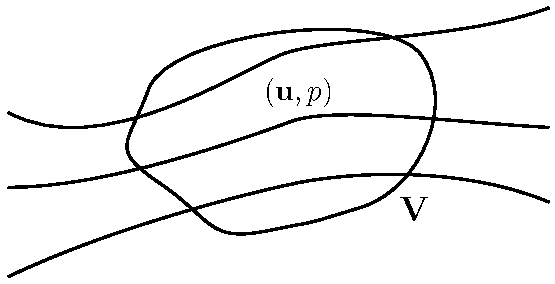
\includegraphics[width=0.4\linewidth]{figures/introduction/eulerianRF.pdf}
		\caption{Eulerian formulation of the fluid. We observe a given volume $\mathbf{V}$ and evaluate the change in properties of the fluid (from incompressible flow: velocity $\mathbf{u}$ and pressure $p$) at time passes.}
		\label{fig:eulerianRF}
	\end{figure}

To ensure more accuracy, one has to solve the Navier-Stokes equation of the flow around the turbine. \indexAcron{Compuational Fluid Dynamic}{CFD} methods discretizes the fluid into smaller regions and solves the set of Navier-Stokes equation in each region (or grids). This type of formulation is known as an Eulerian method as we are evaluating the change in flow property of a given region, figure \ref{fig:eulerianRF}. In order to fully resolve the flow around the turbine, we would have to discretize the fluid at the order of the size of the vortex cores. As the vortex cores are very small (a fraction of size of the airfoil) near the blade, and very large far away from the blade (in order of size of the turbine), we must have grid size that adapts. This requires a large number of grids, as the blades are constantly  moving, and makes it computation very expensive to solve especially for arrays of turbines.

An alternative method is to use the vortex formulation of the Navier-Stokes equations, referred to as vorticity equation. This method is ideal because when describing it in Lagrangian formulation, the vorticity evolution is evaluated as interaction between vortices, and this removes the requirement of gridding, figure \ref{fig:lagrangianRF}. In addition, using simulation acceleration methods such as \indexAcron{Fast Multipole Method}{FMM} and parallel computation in \indexAcron{Graphical Processing Units}{GPU}, they are much more efficient that typical CFD methods and can easily be scaled to distributed computation. However, vortex method cannot inherently take in account the solid body. They require additional methods that can describe the effect of the body in the fluid and the vorticity generated from the body.

	\begin{figure}[!t]
		\centering
		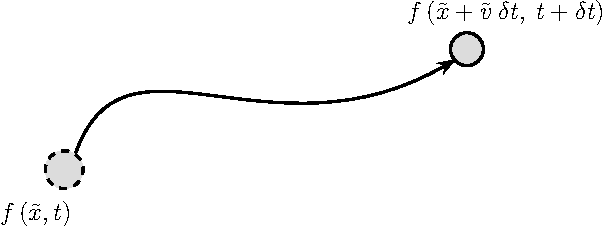
\includegraphics[width=0.4\linewidth]{figures/introduction/lagrangianRF2-crop.pdf}
		\caption{Lagrangian formulation of the fluid. We track the path of the individual fluid elements as time passes.}
		\label{fig:lagrangianRF}
	\end{figure}

So, we see that Eulerian method is accurate when describing the blade-wake interaction but are not efficient when describing multi-scale domains. Whereas, the Lagrangian method is very efficient in evolution the vorticity of the fluid, and is an ideal choice when describing the multi-scale flow characteristics. 

Therefore, in order to use the advantage of both methods, we have decided to use a domain-decomposition method, referred to as \indexAcron{Hybrid Eulerian-Lagrangian Vortex Particle Method}{HVM}. In this method, the Eulerian grid method will be used at the region around the blade (near-wall region). The Lagrangian vortex method will be used in the wake region of the body. With proper coupling of these methods, we can ensure that the this numerical method can capturing not only the near-wake phenomenons such as vortex shedding, dynamic stall, and the wake-body interaction, but also the capture the large-scale flow structures such as the evolution of the VAWT wake, with efficiency and accuracy.

\section{Research Aim and Plan}

\paragraph*{Research Questions:} \textit{Is it possible to develop an efficient and accurate numerical method by an
hybrid approach where the vortex particle method is used in the wake, and the Navier-Stokes grid solver is
used at the near-body region? Will it be able to simulate real life performance characteristics of a vertical
axis wind turbine? Will it be able to predict similar performance characteristics and flow phenomena as observed from the wind tunnel experimental setup? Will it be capable of simulating the blade-wake interaction
and the dynamic stall? Where are the errors and what are their sources?}

\paragraph*{Research aim and plan:}

	\begin{itemize}
	\item Develop the Hybrid method for capturing small-scale phenomenons and large scale phenomenons.
	\item Ensure this tool is efficient, reliable, and accurate.
	\item Verify, Validate the tools with model problems.
	\item Apply the model to the 2D flow of VAWT.
	\end{itemize}

In order to answer this research questions, the goal of the project is the develop an efficient and accurate
numerical method that is not only capable of capture the small scale flow phenomena such as the dynamic stall and the vortex shedding, but is also efficient at modelling the wake evolution of VAWT. The investigation will be performed for 2D geometries and the accuracy of the model needs to established first at simpler problems before continuing to more complex problem cases.

In other words, the initial goal is to develop the hybrid vortex particle method and verify the approach. During this process, the solver will be verified and validated against test cases starting from simpler problems and gradually developing more complex features.

The final goal is to perform a simulation of a VAWT in 2D, compute its performance and validating it against experimental data. By the gradual development of the complex elements of the simulation, one can investigate the feasibility of such approach. Also, the investigation is only done for 2D currently as a full 3D simulation might be difficult and might not be feasible for the master thesis yet.

The innovativeness of this project is that such hybrid modeling has not been yet applied for the wind energy problem case. Through the parallelization of the vortex particle method in a GPU and employing solver acceleration techniques such as the FMM, this simulation could give an edge in the understanding the flow behaviour of a VAWT.

\section{Introduction to Hybrid Eulerian-Lagrangian Vortex Particle Method}

The \indexAcron{Hybrid Eulerian-Lagrangian Vortex Particle Method}{HVM} is a domain-decomposition method, where the Eulerian method and the Lagrangian method solves different domains of the fluid. The domain decomposition method is simply splitting the domain of interest and using the appropriate methods in each domain. For the problem of VAWT, as the boundary is non-trivial and is the source of vorticity, the full Navier-Stokes model will be used here, and away from the body where only the convection of the vorticity field is interested, the fast and efficient vortex particle method will be used, figure \ref{fig:domainDecomposition}.

Several researches have already been done: Cottet and Koumoutsakos (2000a)\cite{Cottet2000a}, Guermond and Lu (2000) \cite{Guermond2000} simulating the advection dominated flows, Ould-Salhi et al. (2001) \cite{Ould-Salihi2001} blending finite difference and vortex method together, Winckelmans et al. (2005a) \cite{Winckelmans2005a} investigating the trailing vorticies, Daeninck (2006) \cite{Daeninck2006} implementing RANS and LES to the simulation, Stock (2010) \cite{Stock} using GPU clusters for efficiency and Speck (2011) \cite{Speck2011a} implementing researching on multipole expansion and modified interpolation kernels.

When evaluating the previous works, we see that not all domain decomposition methods are the same. The main difference differencing between the methods is their coupling strategies. Most works employ the Schwartz alternating method to couple the vortex particle method and the grid solver. The Schwartz alternating method solve the grid solver initially and couples it with the vortex method by iteratively trying to satisfy the boundary conditions. However, for this project the coupling techniques that will be used is similar to Daeninck (2006) \cite{Daeninck2006} and Stock (2010) \cite{Stock}.

	\begin{figure}[!t]
		\centering
		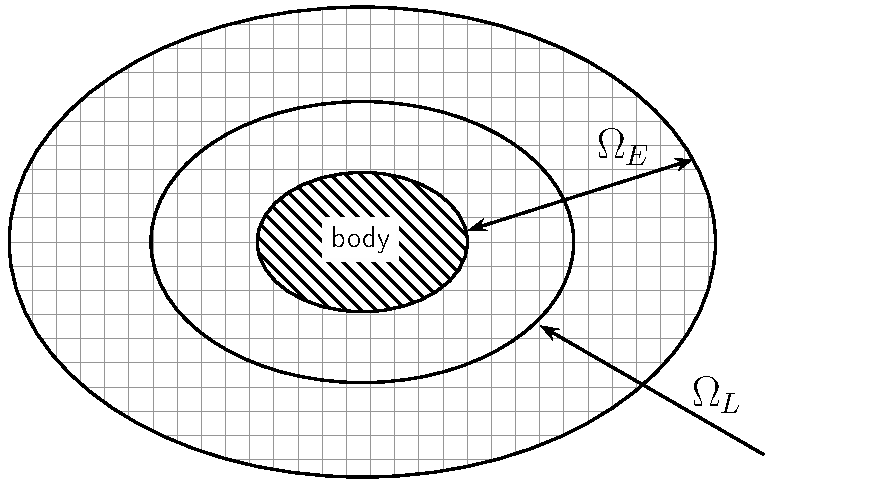
\includegraphics[width=0.5\linewidth]{figures/introduction/domainDecomposition_typical.pdf}
		\caption{Standard domain decomposition using Schwartz iteration for coupling the two methods. Eulerian domain $\Omega_E$ (near the body), and Lagrangian domain $\Omega_L$ (away from the body). Figure is based on Guermond (2000) \cite{Guermond2000}}.
		\label{fig:domainDecomposition}
	\end{figure}

\subsection{Simple coupling strategy}

	\begin{figure}[!b]
		\centering
		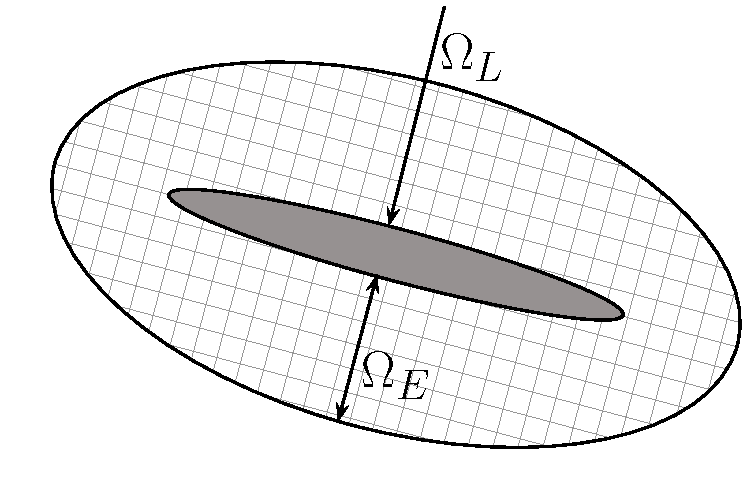
\includegraphics[width=0.5\linewidth]{figures/introduction/domainDecomposition_daenick.pdf}
		\caption{Modified domain decomposition without Schwartz alternating method. Lagrangian domain extends up to the surface of the body. Figure is based on Daeninck (2006) \cite{Daeninck2006}.}
		\label{fig:domainDecomposition_daenick}
	\end{figure}

This new approach is much simpler and only a single iteration is needed for the coupling. The basic procedure is to solve the vortex method in the whole domain using relatively coarse evaluation, then use the grid solver in the near wall region to capture the detailed features of the boundary layer and transfer the vorticity field at this region to the vortex particles, figure \ref{fig:domainDecomposition_daenick}. The functionality of this strategy has been demonstrated by Daeninck and was found to be significantly faster than the Schwartz coupling strategy.

The \underline{features of the simple coupling strategy} can summarized as follows:

	\begin{itemize}
	\item Eulerian method is used to resolve the near-wall region, referred to as Eulerian domain $\Omega_E$. With this implementation, subtle features of the boundary layer (such as flow separation) can be resolved with great accuracy.
	\item Lagrangian method is used to capture the wake, referred to as Lagrangian domain $\Omega_L$. Lagrangian method is used to efficiently evolve the wake.
	\item The accurate solution of the Eulerian domain is transfered to the Lagrangian domain according to the coupling strategies of Daeninck \cite{Daeninck2006} and Stock \cite{Stock}.
	\item The boundary conditions for the Eulerian domain is retrieved from the Lagrangian domain.
	\end{itemize}


	\begin{figure}[!b]
		\centering
		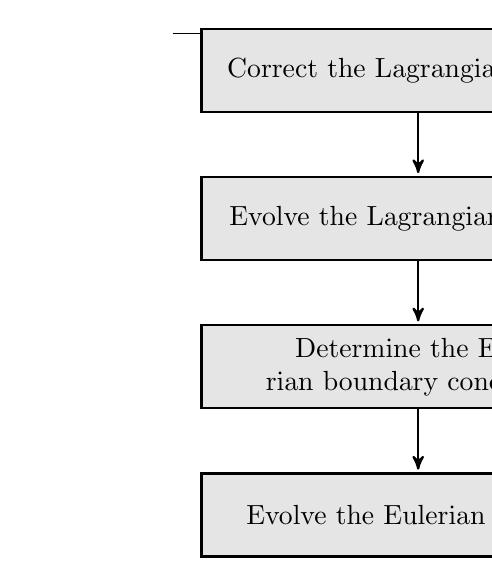
\begin{tikzpicture}
			[node distance=.8cm, start chain=going below,]
			\node[punktchain, join] (correct) {Correct the Lagrangian domain};
		    \node[punktchain, join] (evolveL) {Evolve the Lagrangian solution};
		    \node[punktchain, join] (bcE)     {Determine the Eulerian boundary conditions};
		    \node[punktchain, join] (evolveE) {Evolve the Eulerian solution};
		\end{tikzpicture}
		\caption{Flowchart of the simple coupling strategy. The flowchart shows the procedure to evolve both methods from $t_n$ to $t_{n+1}$.}
		\label{fig:flowchart_simpleCoupling}
	\end{figure}

Figure \ref{fig:flowchart_simpleCoupling} shows the overview to the simple coupling strategy. The detailed algorithm to the simple coupling strategy follows from Daeninck \cite{Daeninck2006}.

The \underline{simple coupling algorithm} can be summarized as follows:

	\begin{enumerate}
	\item \textbf{Correct Lagrangian:} Use the solution of the Eulerian domain $\Omega_E$ (in the near-wall region) to correct the solution of the Lagrangian domain $\Omega_L$ overlapping in the Eulerian domain.  
	\item \textbf{Evolve Lagrangian:} With the modified solution, evolve the Lagrangian solution from $t_n$ to $t_{n+1}$.
	\item \textbf{Determine Eulerian boundary conditions:} Use the Lagrangian solution of $t_n$ and $t_{n+1}$ to determine the boundary conditions of the Eulerian domain.
	\item \textbf{Evolve Eulerian:} With the boundary condition, evolve the Eulerian solution from $t_n$ to $t_{n+1}$.
	\end{enumerate}
	
This is the basic approach for coupling the Eulerian method in the Eulerian domain $\Omega_E$ with the Lagrangian method in the Lagrangian domain $\Omega_L$ without the iterative Schwartz algorithm. In addition, the second difference between the classical hybrid method is that the Lagrangian method handles the boundary conditions differently. Typically during the evolution process of the Lagrangian domain, vorticity is shed from body. However, in this coupling strategy, the Lagrangian method under-resolves the boundary and cannot be used to resolve the vorticity flux. Instead, we use the Eulerian method to resolve the boundary and interpolate the newly generated vorticity into the Lagrangian domain.

However, there as some \underline{assumptions} that we must satisfy, for this coupling strategy to be valid:

	\begin{enumerate}
	\item At $t_n$, before the evolution of both method to $t_{n+1}$, the Lagrangian solution matches Eulerian solution at the near-wall region.
	\item After the evolution to $t_{n+1}$, the deviation of the Lagrangian solution (due to lack of vorticity flux at Lagrangian boundary), is minimal.
	\item Even though the Lagrangian domain is under-resolved in the near-wall region, it should be able to provide accurate boundary conditions for the Eulerian external boundary.
	\end{enumerate}


\section{Verification and Validation Test Cases}

The test-cases that are used for this thesis are summarized as given:

	\begin{description}
	\item[Lamb-Oseen vortex] \cite{Lamb1993} \cite{Tryggeson2007} \hfill\\
	Lamb-Oseen vortex test case is an analytical solution derived from the diffusion equation, and is a test case for unbounded flow (without any wall). This is the first model that will be used to validate the Lagrangian method and Eulerian method separately. This test case focuses on the diffusion of the vortcity is an ideal to verify and validate the convection and diffusion of the vorticity.
	\item[Clercx-Bruneau dipole] \cite{Clercx2006}\hfill\\
	The Clercx-Bruneau dipole test case is the simple case of dipole colliding with a wall and is used to verify the coupling of the methods. This test cases focuses on the generation of vorticity from the wall and is ideal to verify and validate the coupling.
	\item[Impulsively started cylinder] \cite{LEONARD1995} \cite{Chang2006} \cite{Chassaing1986} \cite{Lecointe1985}\hfill\\
	The impulsively started cylinder test case focuses on the forces acting on the cylinder. This test case is used to verify and validate the lift and drag evolution of the cylinder exposed to free-stream flow.
	\item[Elliptic Airfoil] \cite{Nair1997}\hfill\\
	The elliptic airfoil test cases focuses on the flow separation past a lifting body. The elliptic airfoil is pitched at high angle of attack and the flow past the airfoil is comparatively unsteady and undergoes phenomenons such as laminar separation bubble, flow separation and karman vortex shedding from the trailing edge of the airfoil. This helps us ensure coupling process is sound for complex flow phenomenons.
	\end{description}

%\todo{add picture here}
\section{Methodology}
The initial steps of the development of the hybrid vortex methods is as follows:

	\begin{itemize}
	\item Develop the vortex particle method
	\item Validate the vortex particle method against a Lamb-Oseen convection test case.
	\item Develop the vortex panel method to deal with the boundaries for the vortex particle calculation. 
	\item Validate the vortex panel method by solving a potential flow around a cylinder.
	\item Develop the grid solver that is based on the Finite Element method. 
	\item Validate the grid solver against test cases: impulsively starting cylinder, dipole-Wall interaction.
	\end{itemize}

Once all the components have been validated, the methods will be coupled and validated against similar test cases.

	\begin{itemize}
	\item Couple vortex particle, vortex panel and grid solver together.
	\item Validate it with the previous generated test case solution.
	\item Introduce more complicated phenomenons: multiple geometry (i.e multiple grid meshes) and moving boundaries, if it feasible in the constraints of a master thesis.
	\end{itemize}

If the coupled solver has been validated with the test cases, the final step will be to simulated the flow around a VAWT and investigating the performance vs. numerical and experimental data.

%\subsection{Project Plan}

\section{Thesis Outline}

\todo{Update this section}

%\section{Research question}
%\label{sec:ResearchQuestion}
%
%\section{Research objective}
%\label{sec:ResearchObjective}
%
%\section{Importance of study}
%
%\section{Scope of thesis}
%\label{sec:scope}
%
%\section{Structure of the report}
%\label{sec:Structure of the report}

%

	% Chapter 2: Hybrid Eulerian-Lagrangian Vortex Particle Method
  	\chapter{Hybrid Eulerian-Lagrangian Vortex Particle Method}
\label{ch:helvpm}

% Summarize the sections. : domain decomposition, coordinate systems assosciated to each
% subdomains, and the coupled evolution of the hybrid method.
% Reference to the literatures: Cottet and others, stock and daenick
% We use approach of stock based on the phd research of daeninck

	\section{Introduction to Hybrid Eulerian-Lagrangian Vortex Particle Method}
	
	The \printAcron{Hybrid Eulerian-Lagrangian Vortex Particle Method}{HELVPM} is a domain decomposition method, where the Eulerian method and the Lagrangian method solves different regions of the fluid. The domain decomposition method simply splits the domain of interest and uses appropriate method in each domain. The Eulerian formulation will be used at the near-wall region, where we need proper description of the vorticity generation at the boundary, and the Lagrangian formulation is used away from the body, where we only need to evolve the vorticity field. Figure \ref{fig:domainDecomposition} shows the decomposition of the domain to the gridded and the non-gridded region.
	
		\begin{figure}[!h]
			\centering
			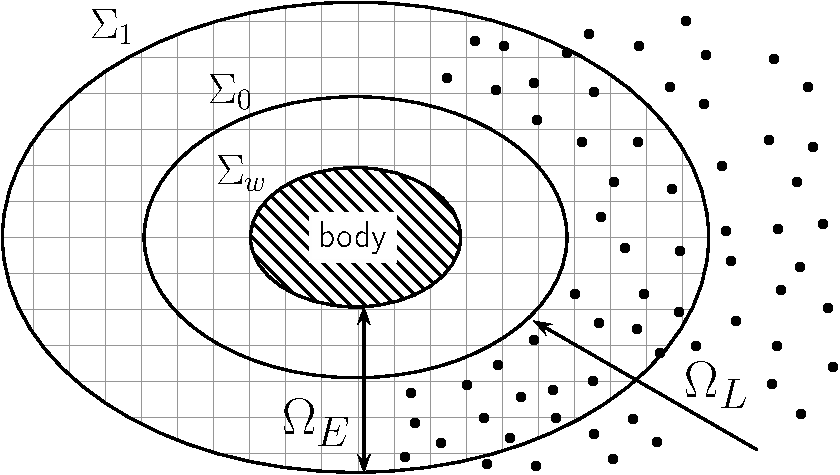
\includegraphics[width=0.6\linewidth]{figures/hybrid/domainDecomposition_typical_type2-crop.pdf}
			\caption{Standard domain decomposition using Schwartz iteration for coupling the two methods. Eulerian subdomain $\Omega_E$ (near the body), and Lagrangian subdomain $\Omega_L$ (away from the body). Figure is based on Guermond (2000) \cite{Guermond2000a}.}
			\label{fig:domainDecomposition}
		\end{figure}	
	
	Several studies have already been done: Cottet and Koumoutsakos (2000a)\cite{Cottet2000a}, Guermond and Lu (2000) \cite{Guermond2000a} simulated the advection dominated flows; Ould-Salhi et al. (2001) \cite{Ould-Salihi2001a} blended the finite difference and vortex method together; Winckelmans et al. (2005a) \cite{Winckelmans2005} investigated the trailing vorticies; Daeninck (2006) \cite{Daeninck2006} used a simplified coupling strategy, coupling Vortex Particle Method and Finite Diference Method; Stock (2010) \cite{Stock2010a} expanded Daeninck's strategy, coupling Vortex Particle Method and Finite Volume Method and modeled a 3D rotor.

	\section{Convectional Coupling Strategy}
	\label{sec:helvpm-ccs}
	
	When investigating the literature works, we see that not all domain decomposition methods are the same. The main difference between the methods is their coupling strategies. Most works employ the\textit{ Schwartz alternating method} to couple the vortex particle method and the grid solver. The Schwartz alternating method (or sometimes referred to as Schwartz iterative method), couples the vortex particle method and the grid solver by iteratively determining the boundary condition such that the stream functions in both domains, $\psi_L$ and $\psi_E$ in $\Omega_L$ and $\Omega_E$ respectively, match at the overlap region $\Omega_E-\Omega_L$, shown in Figure \ref{fig:domainDecomposition}. The summary of a single iteration of the Schwartz alternating method is as follows:
	
		\begin{itemize}
		\item Determine the Eulerian boundary condition, the stream function $\psi_{\Sigma_1}$ at the Eulerian boundary $\Sigma_1$, extracted from the Lagrangian stream function $\psi_L$ in the Lagrangian subdomain $\Omega_L$.
		\item Solve for the stream function $\psi_E$ in the Eulerian subdomain $\Omega_E$ with the new boundary condition $\Sigma_1$.
		\item Determine the Lagrangian condition, the stream function $\psi_{\Sigma_0}$ at the Lagrangian boundary $\Sigma_0$, extracted from the Eulerian stream function $\psi_E$ in the Eulerian subdomain $\Omega_E$.
		\item Solve the stream function $\psi_L$ in the Lagrangian subdomain with the boundary conditions $\psi_{\Sigma_0}$ at the Lagrangian boundary $\Sigma_0$.
		\end{itemize}
	
	This procedure is iterated until the stream functions of both domains converge \cite{Ould-Salihi2001a}. Once the stream function is determined in both the domains, the velocity field can be obtained. Using the velocity field, we can then evolve the vorticity field in the Lagrangian subdomain.

	\section{Simplified Coupling Strategy}
	\label{sec:helvpm-scs}
	
	As we realized now, the downside to this procedure is that we have to solve the stream function in both $\Omega_E$ and $\Omega_L$ iteratively, until we converge to a solution. This makes the computation very expensive, especially when we are dealing with large numbers of vortex particles. Therefore, for this project, we are using the coupling technique that is based on the research work of Daeninck (2006) \cite{Daeninck2006} and Stock (2010) \cite{Stock2010a}. However, through the course of present work, we will see that we have to perform a modification to the scheme, to ensure that the total circulation of the Lagrangian domain is conserved at all times.	
	
%	\subsection{Coupling Eulerian and Lagrangian Methods}
	
	The simplified coupling strategy was first demonstrated in the doctoral thesis of Daeninck \cite{Daeninck2006}. Daeninck showed that it is possible to coupled the Lagrangian and the Eulerian method without the use of Schwartz iterative method. Daeninck proposed this approach from the following statements:
	
	\begin{itemize}
	\item The Lagrangian vortex method solves the full fluid domain $\Omega_L$ (see Figure \ref{fig:domainDecomposition_daenick}), but under-resolves the near-wall region $\Omega_E$ as it is less efficient at resolving the boundary layer of the flow.
	
	\item Eulerian method is used to resolve the near-wall region $\Omega_E$, efficiently capturing the boundary layer features and flow separation.
	
	\item The Lagrangian subdomain in the near-wall region $\Omega_L\cap\Omega_E$ is corrected using the more accurate Eulerian solutions to compensate the aforementioned under-resolution.
	
	\item The boundary conditions for the Eulerian method is directly obtained from the evolved solution of the Lagrangian method.
	\end{itemize}
	
	The grid solver therefore essentially acts as the correction for the under-resolved regions of the Lagrangian method. The Lagrangian vortex method in the full fluid domain focuses only on capturing and efficiently evolving the wake.
	
		\begin{figure}[!h]
			\centering
			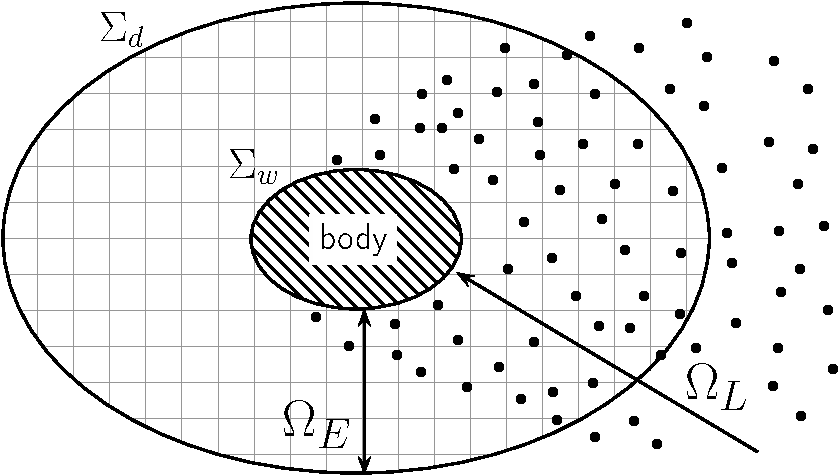
\includegraphics[width=0.6\linewidth]{figures/hybrid/domainDecomposition_daenick_type2-crop.pdf}
			\caption{Modified domain decomposition \underline{without} Schwartz alternating method. Lagrangian subdomain extends up to the surface of the body. Figure is based on Daeninck (2006) \cite{Daeninck2006}.}
			\label{fig:domainDecomposition_daenick}
		\end{figure}	
	
	Furthermore, Daeninck's simplified coupling strategy handles the Lagrangian boundary condition differently from the convectional domain decomposition method. In convectional method, the shedding of the vorticity from the wall is also defined in the Lagrangian method as well. However, in Daeninck's strategy, as the Lagrangian method is under-resolved at the boundary, it cannot be used to resolve the vorticity flux at the body. Instead, the Eulerian method is used to solve vorticity generation from the wall boundary, and acts as the vorticity generator for the Lagrangian method. 
	
	For this coupling strategy to be valid, there are some assumptions that we must satisfy:

	\begin{itemize}
	\item At $t_n$ before the evolution of both method to $t_{n+1}$, the Lagrangian solution matches Eulerian solution at the boundary of the near-wall region $\Sigma_d$ (see Figure \ref{fig:domainDecomposition_daenick}).
	\item Even though the Lagrangian subdomain is under-resolved in the near-wall region, it should still be able to provide accurate boundary conditions for the Eulerian method at the external boundary $\Sigma_d$.
	\item After the evolution to $t_{n+1}$, the deviation of the Lagrangian solution (due to lack of vorticity flux at Lagrangian boundary), should be minimal.
	\end{itemize}	
	
	Daeninck's the simplified coupling strategy focused on the vorticity-velocity formulation for the Eulerian domain. However, he briefly showed that it is also possible to couple the Eulerian method with the velocity-pressure formulation. The advantage of using the velocity-pressure formulation is that it will be easier to extend to a 3D problem, unlike the vorticity-velocity formulation for the Eulerian method.
	
	\subsection{Coupling Algorithm}	
	
	The coupling of the solvers was described in one global time stepping algorithm. As the Eulerian methods suffers from a larger stability constraint on the time step, and the Lagrangian time marching is computationally more expensive, a  different time discretization for both methods was employed. The Lagrangian method and the Eulerian method had the time steps $\Delta t_L$ and $\Delta t_E=\Delta t_L/k_E$, respectively, where $k_E$ is the number of Eulerian sub-steps.
	
	Assuming that we known the solutions of both solver at $t_n$, the algorithm for the coupled time marching from $t_n$ to $t_n+\Delta t_L$ for Eulerian method (with velocity-pressure formulation) and the Lagrangian method is summarized as follows:
	
	\begin{enumerate}
	\item At $t_n$, \textbf{correct the Lagrangian solution} in the near-wall region $\Omega_L\cap\Omega_E$ from the Eulerian field, Figure \ref{fig:domainDecomposition_daenick}. The vorticity in $\Omega_E$ is determined by taking the curl of the velocity field of the Eulerian method. The vortex particles strengths are determined by interpolating the vorticity from the Eulerian grid.
	
	\item \textbf{Advance the Lagrangian method} from $t_n$ to $t_{n}+\Delta t_L$, with the corrected Lagrangian solution. Before the evolution, there exists a slip velocity at the solid wall $\Sigma_w$. Therefore, the vortex method needs to enforce the \textit{no-slip} boundary condition at the wall by computing the vortex sheet $\gamma$ that cancels this slip velocity. At the end of the evolution, classic vortex methods diffuse the computed vortex sheet to the particles but in Daeninck's work, it is handled by the Eulerian method.
	
	\item\textbf{ Determine the Eulerian boundary conditions} for the velocity field $\mathbf{u}$ at $t_{n}+\Delta t_L$ from the Lagrangian solution at $t_{n} + \Delta t_L$. The Eulerian method requires the Dirichlet velocity boundary condition at $\Sigma_d$ (the Eulerian Dirichlet velocity boundary). The velocity boundary condition at the wall boundary $\Sigma_w$ for a velocity-pressure formulation is simply the zero slip velocity. 
	
	\item \textbf{Advance the Eulerian method} from $t_n$ to $t_n + \Delta t_L$ using $k_E$ Eulerian substeps. The boundary conditions on $\mathbf{u}$ at each substep is obtained by linear interpolation of the boundary condition at $t_n$ and $t_{n} + \Delta t_L$.
	\end{enumerate}	
	
	To enhance the coupling of the Eulerian and the Lagrangian method, Daeninck further modified the Eulerian solution in the most external region of the Eulerian subdomain $\Omega_E$ from interpolation the Lagrangian solution, and observed that it provided better results. Figure \ref{fig:daeninckInterpolation} the modified adjustments regions used by Daeninck in his work.
	
	\begin{figure}[!t]
		\centering
		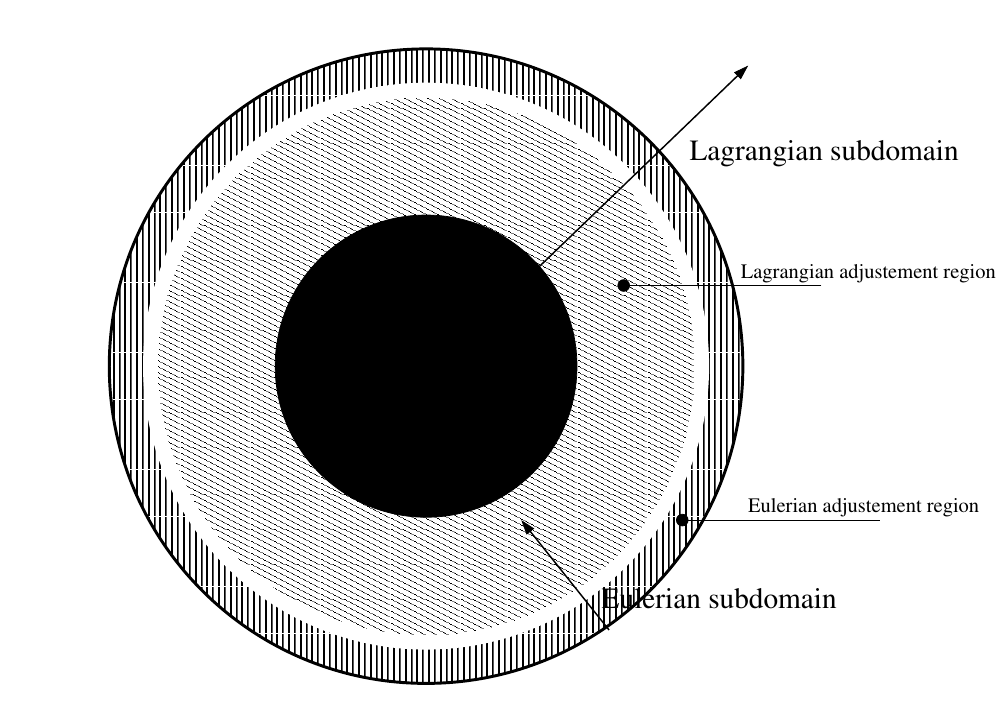
\includegraphics[width=0.6\linewidth]{figures/hybrid/daeninckInterpolationRegions.png}
		\caption{The domain decomposition and interpolation regions used by Daeninck \cite{Daeninck2006}. The Eulerian domain is also modified to enchace the coupling of the methods.}
		\label{fig:daeninckInterpolation}
	\end{figure}		
	
	\subsection{Lagrangian Correction Step}
	
	The coupling strategy demonstrated by Daeninck \cite{Daeninck2006}, was studied and was further extended by Stock \cite{Stock2010a}. Stock's work focused on the overlap region $\Omega_E\cap\Omega_L$ (Figure \ref{fig:domainDecomposition_daenick}) and correction of the Lagrangian solution. Following observations was determined by the work:
	
	\begin{itemize}
	\item Eulerian solution is only assumed to be correct from the body surface $\Sigma_w$ to somewhat inside of the outer Eulerian domain $\Sigma_d$. Therefore, the transfer of the Eulerian solution to the Lagrangian method should take in account of the potential inaccuracy of the Eulerian solution at the outer boundary.
	
	\item The very strong gradient in vorticity (vortex sheet) cannot be efficiently and accurately transfered to the Lagrangian method. This is especially problematic at high Reynolds number flows, and interpolating this vorticity from Eulerian method to Lagrangian method results in numerical problems. Therefore, to avoid the noise in the interpolation, the correction step has to ignore the region very near to the wall.
	\end{itemize}
	
	The resulting Lagrangian correction domain, or the interpolation domain $\Omega_I$, using Stock's coupling approach is shown in Figure \ref{fig:interpolationDomainDefinition}. The interpolation domain $\Omega_I$ is defined with an offset from the Eulerian domain boundaries $\Omega_E: \partial\Omega_E=\Sigma_w \cup \Sigma_d$, Figure \ref{fig:interpolationDomainExpanded}, such that regions of the Eulerian domain that introduces issues with coupling are ignored. The outer boundary of the interpolation domain $\Sigma_i$ is defined with an offset $d_{bdry}$ from the Eulerian Dirichlet velocity boundary $\Sigma_d$ such that potential inaccuracy of the Eulerian solution is ignored, shown in Figure \ref{fig:interpolationDomainCloseup}. Similarly, the inner boundary of the interpolation domain $\Sigma_o$ is defined with an offset $d_{surf}$ from the Eulerian wall boundary $\Sigma_w$ such that the very strong vorticity is ignored. The offsets $d_{surf}$ and $d_{bdry}$  where defined in the order of the Lagrangian vortex particle size.
	
	\begin{figure}[!t]
        \centering
        \begin{subfigure}[b]{0.45\textwidth}
                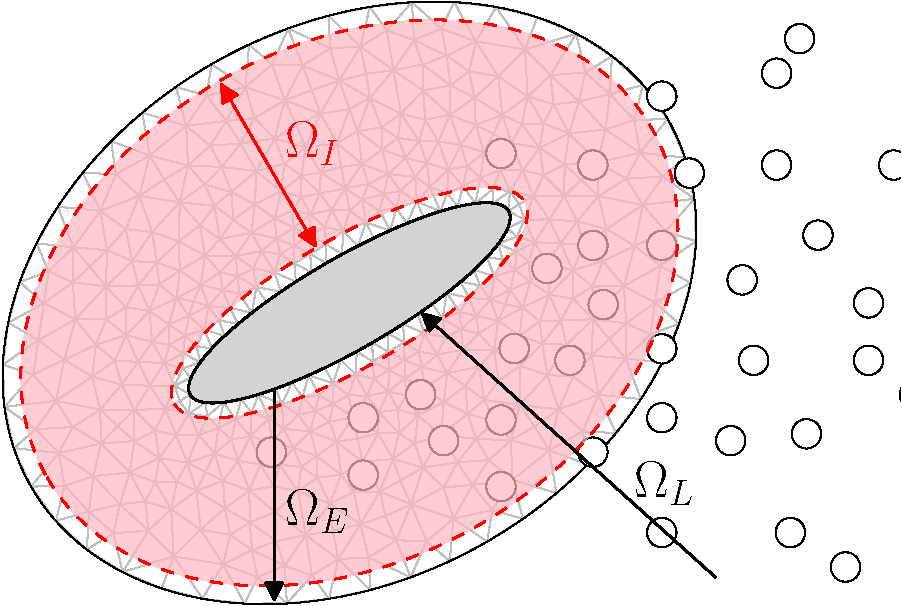
\includegraphics[width=\textwidth]{figures/hybrid/interpolationDomain/interpolationDomainExpanded-crop.pdf}
                \caption{Definition of the Domains}
                \label{fig:interpolationDomainExpanded}
        \end{subfigure}%
        \qquad %add desired spacing between images, e. g. ~, \quad, \qquad etc.
          %(or a blank line to force the subfigure onto a new line)
        \begin{subfigure}[b]{0.45\textwidth}
                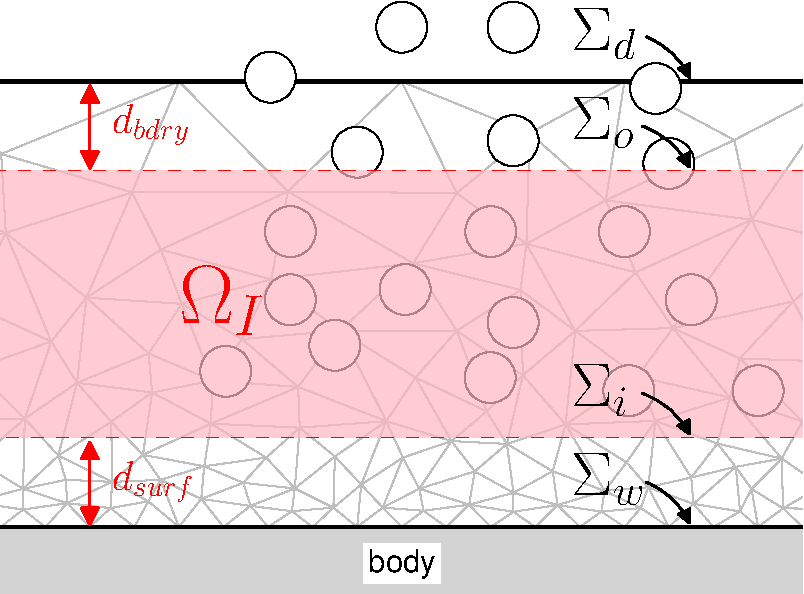
\includegraphics[width=\textwidth]{figures/hybrid/interpolationDomain/interpolationDomainCloseup-crop.pdf}
                \caption{Definition of the boundaries}
                \label{fig:interpolationDomainCloseup}
        \end{subfigure}
        \caption{Definition of the interpolation domain $\Omega_{int}$ for correcting the Lagrangian solution, with boundaries $\Omega_I: \partial\Omega_I=\Sigma_{i}\cup\Sigma_{o}$.}
        \label{fig:interpolationDomainDefinition}
	\end{figure}		

	The resulting Lagrangian correction step employed by Stock is summarized as follows:
	
	\begin{enumerate}
	\item Interpolate the vorticity of the Eulerian method from a non-uniformly structured (or an unstructured grid) onto a temporary uniformly structured Cartesian grid covering the entire Eulerian domain $\Omega_E$. This is done to performed an easier correction of the Lagrangian solution with the Eulerian solution. The interpolation ignores the very strong vorticity present in the boundary layer that could cause numerical problem.
	\item Determine all the particles within the interpolation domain $\Omega_I$ that is to be corrected.
	\item Correct or reset the strengths of the particles using the local particle area and the vorticity interpolated from the temporary structured Cartesian grid.
	\end{enumerate}
	
	Using this approach, Stock demonstrated the feasibility of simulating a 3D compressible flow problem around a sphere at $Re=100$, a finite airfoil at $Re=\num{1.5e6}$, and 4-Bladed advancing rotor at $Re=865,500$.
	
	\section{Evolution of the Hybrid Method}

	In the present work, we will therefore employ Daeninck's simplified coupling strategy with the detailed Lagrangian correction approach of the Stock. The evolution of the hybrid method is classified into four parts and is as follows:

		\begin{enumerate}
		\item \textbf{Correct Lagrangian:} Use the solution of the Eulerian subdomain $\Omega_E$, to correct the solution of the Lagrangian subdomain $\Omega_L$, using the strategy of Stock. Chapter \ref{ch:coupling} provides a detailed investigation on the implementation of Stock's Lagrangian correction strategy. However, during the implementation, we saw that conservation of total circulation in the Lagrangian method is paramount for an accurate correction.
		
		\item \textbf{Evolve Lagrangian:} With the modified solution, evolve the Lagrangian solution from time step $t_n$ to $t_{n}+\Delta t_L$. Chapter \ref{ch:lagrangian} provides the detailed investigation on the theory and the algorithm of the Lagrangian method used for the present work.
		
		\item \textbf{Determine Eulerian boundary conditions:} Use the Lagrangian solution of time $t_{n}+\Delta t_L$ to determine the boundary conditions of the Eulerian subdomain at $t_{n}+\Delta t_L$.
		
		\item \textbf{Evolve Eulerian:} With the boundary condition, evolve the Eulerian solution from $t_n$ to $t_{n}+\Delta t_L$ using $k_E$ Eulerian substeps. Chapter \ref{ch:eulerian} provides the detailed investigation on the theory and the algorithm of the Eulerian method used for the present work.
		\end{enumerate}
	
	Figure \ref{fig:flowchart_simpleCoupling} shows the flowchart of the evolution of the hybrid method. To ensure that the coupling of the hybrid method performs as explained in theory, we required a verification and validation test on the functionality of each segregate methods.
	
	
	\begin{figure}[!t]
		\centering
		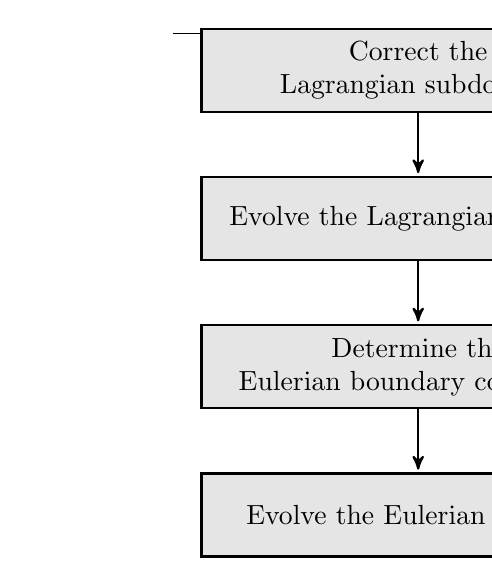
\begin{tikzpicture}
			[node distance=.8cm, start chain=going below,]
			\node[punktchain, join] (correct) {Correct the \\Lagrangian subdomain};
		    \node[punktchain, join] (evolveL) {Evolve the Lagrangian solution};
		    \node[punktchain, join] (bcE)     {Determine the \\Eulerian boundary conditions};
		    \node[punktchain, join] (evolveE) {Evolve the Eulerian solution};
		\end{tikzpicture}
		\caption{Flowchart of the simple coupling strategy. The flowchart shows the procedure to evolve both methods from $t_n$ to $t_{n+1}$.}
		\label{fig:flowchart_simpleCoupling}
	\end{figure}




% Summarize daenincks approach:
	% Methodology, algorithm
	% Domain decomposition
% Summarize stock's approach:
	% Methodology, algorithms
	% Resulted domain decomposition.

    % Chapter 3 : Lagrangian Subdomain: Vortex Particle Method
	\chapter{Lagrangian Method: Vortex Particle Method}
\label{ch:lagrangian}

	
%	\lsymb[f]{$\mathbf{x}$}{Position vector}{\si{\m}}{x}
%	\lsymb[f]{$\mathbf{x}_p$}{Position vector of the particle}{\si{\m}}{xp}
%	\lsymb[f]{$\mathbf{x}_{\nu}$}{Position vector of particle to be diffused}{\si{\m}}{xmm}
%	\lsymb[f]{$t$}{Time}{\si{\s}}{t}
%	\lsymb[f]{$\mathbf{u}$}{Velocity}{\si{\m\per\s}}{u}
%	%\lsymb[f]{$\mathbf{u}\left(\mathbf{x},t\right)$}{Velocity field}{$[m\cdot s^{-1}]$}{ua}
%	\lsymb[f]{$p$}{Pressure}{\si{\pascal}}{p}
%	\lsymb[f]{$\mathbf{u}^h$}{Discrete velocity}{\si{\m\per\s}}{uh}	
%	\lsymb[f]{$\mathbf{u}_{\infty}$}{Free-stream velocity}{\si{\m\per\s}}{ul}
%	\lsymb[f]{$\mathbf{u}_{\omega}$}{Vortical velocity}{\si{\m\per\s}}{uz}
%	\lsymb[f]{$\mathbf{u}_{\phi}$}{Potential velocity}{\si{\m\per\s}}{up}
%	\lsymb[f]{$\mathbf{u}_{\gamma}$}{Vortex sheet induced velocity}{\si{\m\per\s}}{uc}
%	\lsymb[f]{$\mathbf{u}_{\mathrm{ext}}$}{External induced velocity}{\si{\m\per\s}}{ue}
%	\lsymb[f]{$\mathbf{u}_{b}$}{Velocity of the body}{\si{\m\per\s}}{ub}	
%	\lsymb[f]{$\mathbf{u}_{\mathrm{slip}}$}{Boundary slip velocity}{\si{\m\per\s}}{us}	
%	\lsymb[f]{$u_{r}$}{Radial velocity}{\si{\m\per\s}}{ur}	
%	\lsymb[f]{$u_{\theta}$}{Angular velocity}{\si{\m\per\s}}{uhh}	
%
%		
%	\lsymb[f]{$N_p$}{Number of particles}{-}{np}	
%	\lsymb[f]{$\mathbf{K}$}{Biot-Savart kernel}{-}{k}
%	\lsymb[f]{$\mathbf{K_{\sigma}}$}{Vortex blob kernel}{-}{kb}	
%	\lsymb[f]{$h$}{Nominal particle spacing}{\si{m}}{h}	
%	\lsymb[f]{$\mathrm{overlap}$}{Overlap ratio of the blobs}{-}{o}	
%	\lsymb[f]{$W$}{Interpolation kernel weight}{-}{w}
%	\lsymb[f]{$\mathcal{E}$}{Enstrophy}{\si{m^2.s^{-2}}}{en}
%	\lsymb[f]{$c^2$}{Diffusion parameter}{-}{c}
%	\lsymb[f]{$\mathbf{\hat{n}}$}{Normal vector}{-}{n}
%	\lsymb[f]{$\mathbf{\hat{s}}$}{Tangent vector}{-}{s}	
%	\lsymb[f]{$h_{\nu}$}{Characteristic diffusion distance}{\si{m}}{hm}		
%	\lsymb[f]{$k_{d}$}{Diffusion frequency multiple}{-}{kd}			
%	
%	\lsymb[f]{$\mathbf{A}$}{Vortex panel influence matrix}{-}{kd}				
%
%	\lsymb[f]{$r$}{Radial position}{\si{m}}{r}
%
%	\gsymb[f]{$\zeta_{\sigma}$}{Smooth cut-off function of the blob}{-}{ff}	
%	\gsymb[f]{$\rho$}{Density}{\si{kg.m^{-3}}}{qq}
%	\gsymb[f]{$\nu$}{Kinematic viscosity}{\si{m^2.s^{-1}}}{mm}
%	\gsymb[f]{$\Gamma$}{Circulation}{\si{m^2.s^{-1}}}{c}
%	\gsymb[f]{$\Gamma_{\omega}$}{Circulation of the fluid}{\si{m^2.s^{-1}}}{cxx}	
%	\gsymb[f]{$\Gamma_{\gamma}$}{Circulation of vortex sheet}{\si{m^2.s^{-1}}}{ccc}		
%	\gsymb[f]{$\Gamma_{b}$}{Circulation of moving body}{\si{m^2.s^{-1}}}{cb}			
%	\gsymb[f]{$\omega$}{Vorticity}{\si{s^{-1}}}{xx}
%	\gsymb[f]{$\omega^h$}{Discrete vorticity field}{\si{s^{-1}}}{xxh}
%	\gsymb[f]{$\alpha_p$}{Circulation of the particle}{\si{m^2.s^{-1}}}{aap}
%	\gsymb[f]{$\beta_p$}{Corrected circulation of the particle}{\si{m^2.s^{-1}}}{bbp}
%	%\gsymb[f]{$\epsilon$}{Distance between the particles}{$[m]$}{eep}
%	\gsymb[f]{$\sigma$}{Core size}{\si{m}}{rr}
%	\gsymb[f]{$\Delta t_d$}{Diffusion time-step size}{\si{s}}{dtd}	
%	\gsymb[f]{$\Delta t_c$}{Convection time-step size}{\si{s}}{dtc}		
%	\gsymb[f]{$\gamma$}{Vortex sheet strengths}{\si{s}}{cc}		
%	\gsymb[f]{$\xi$}{Scale relative position of particle to stencil node}{-}{nn}
%	\gsymb[f]{$\epsilon$}{Relative error}{-}{ee}
%	\gsymb[f]{$\tau$}{Scaled viscous time}{\si{m^2}}{ss}
%	\gsymb[f]{$\Gamma_c$}{Circulation of the vortex core}{\si{m^2.s^{-1}}}{cc}

%To model the flow around a VAWT, several approaches can be taken, Vermeer at al. (2003) \cite{Vermeer2003} have also summarized in their paper. The two main approaches of investigating the flow is either employing a numerical method to simulate the flow or through experimental simulations.

%Leishman (2006) \cite{leishman2006principles} has shown that there are several simplified, efficient numerical tools that can be used to model the performance of a VAWT. Methods such as actuator disk theory and blade element momentum theory and deals with simplified Navier-Stokes equations and is very useful to evaluate the trend of certain design parameter. However, as they are highly simplified, complex flow phenomenons that has severe impact of the performance characteristics of the VAWT such as flow separation during dynamic stall, vortex shedding during the rotation and blade-wake interaction cannot be simulated. In order to understand them, either experimental investigation such as in wind tunnel or full Navier-Stokes simulations have to undertaken. So to understand the flow behaviour of a VAWT, several numerical research have been performed \cite{Almohammadi2013} \cite{Ferreira2007} \cite{Islam2008} \cite{Merz2012} and experimental researches by Ferreira \cite{SimaoFerreira2008} \cite{Ferreira} and others \cite{Howell2010} \cite{Mertens2003}.
%\index{Actuator disk}

%All the numerical method that was grid-based struggled with dealing with large number of mesh cells for high Reynolds numbers and the numerical method that employed simplified Navier-Stokes methods had to sacrifices some accuracies.The experimental investigation also come with drawbacks as they are require more financial resources and usually only feasible to model the scaled VAWTs.

%This is the main relevance of the hybrid vortex particle method for the VAWT investigations. By utilizing the two methods together, the vortex particle method away from body, and Navier-Stokes solver with turbulence model in the near-body region, one will be able to tackle the challenges in an efficient manner.

%Therefore, this chapter is dedicated to given an overview on the theory of the Vortex Particle Method which we will employ with coupled Navier-Stokes solver. 

%------------------------------------------------------------------------------------------------------
%------------------------------------------------------------------------------------------------------
%------------------------------------------------------------------------------------------------------
\section{Introduction to the Vortex Particle Method}
\label{sec:introtovpm}
\indexAcron{Vortex Particle Method}{VPM} is a numerical method employed in computational fluid dynamics, dealing with the evolution of the vorticity in the fluid from a Lagrangian description. In an Eulerian formulation, the fluid is viewed at a fixed window where the change in the fluid properties are evaluated. However, the Lagrangian formulation, regards the fluid as a collection of particles (or elements) carrying properties of the fluid (such as vorticity, mass, etc.). 

Efficient discretization of the fluid domain becomes a difficult task for cases such as \printAcron{Vertical-Axis Wind Turbine}{VAWT}, where the wake geometry is complex and unsteady. Discretizing such wake using Eulerian formulation becomes difficult as it requires the adaption of the mesh over time for efficient computation. The VPM only needs fluid elements where there is vorticity meaning that the method is inherently auto-adaptive. This is one of the advantage of the VPM. Furthermore, with computational acceleration methods such as \printAcron{Fast-Multipole Method}{FMM} and parallel computation in \printAcron{Graphics Processing Units}{GPU} enables an efficient evolution of the vorticity wake. 

However, the key advantage of the VPM is that it is ideal for capturing the resolving the long-time characteristics of the unsteady compact vortical structures that are shed off from the VAWT blades, as described by Stock \cite{Stock2010a}, providing the motivation for using VPM for modeling the rotor wake.

A summary of the advantage of the Lagrangian vortex method w.r.t the Eulerian method was provided by Wee and Ghoniem \cite{Wee2006a}:
\begin{itemize}
\item Eulerian methods introduce dissipation, even in flows with zero velocity gradient. However such error as minimized at the convection of the Lagrangian method.
\item The numerical stability of the Lagrangian method is not restricted by the CFL condition.
\item The support of the Lagrangian elements are a small fraction of the fluid domain. The support is confined to location of non-zero vorticity, making the method naturally grid adaptive.
\end{itemize}

The main literature on the VPM (the Lagrangian component of the hybrid method), is the book of Cottet and Koumoutsakos, Vortex Methods: Theory and Practice \cite{Cottet2000a}. It gives an insight on the fundamentals of the vortex method (specifically VPM) and gives a summary on hybrid methods.

\subsection{Vorticity}
The vorticity $\omega$ is the governing element of the VPM. It is given by
	\begin{equation}
	\mathbf{\omega} = \nabla \times \mathbf{u},
	\label{eq:lag_vort}
	\end{equation}
where $\mathbf{u}$ is the velocity vector field. In 2D, the circulation $\Gamma$ is defined by Stokes' theorem as,

	\begin{equation}
	\Gamma = \int_L\mathbf{u}\cdot \mathrm{d}s= \int_A (\nabla \times \mathbf{u}) \cdot \mathbf{n}\ \mathrm{d}A = \int_A\omega\cdot\mathbf{n}\ \mathrm{d}A,
	\label{eq:definitionOfCirculation}
	\end{equation}

and represents the flux integral of vorticity across the surface $A$, contoured by the line $s$. Figure \ref{fig:vorticityCirculation} depicts this relation of velocity $\mathbf{u}$, vorticity $\omega$ and the circulation $\Gamma$.

	\begin{figure}[!h]
	\centering
	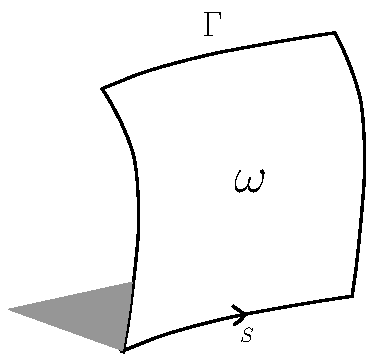
\includegraphics[width=0.3\linewidth]{./figures/lagrangian/vorticityCirculation_updated.pdf}
	\caption{Definition of the circulation in the fluid.}
	\label{fig:vorticityCirculation}
	\end{figure}

 
\subsection{Velocity-Vorticity formulation of the Navier-Stokes equations}
The governing equation of the vortex particle method is the velocity-vorticity formulation $\mathbf{u}-\omega$ of the Navier-Stokes equations, as presented in Cottet and Koumoutsakos \cite{Cottet2000a}. It is derived from the 2D incompressible Navier-Stokes momentum equation, given as,
	\begin{equation}
	\frac{\partial \mathbf{u}}{\partial t} + \mathbf{u}\cdot\nabla\mathbf{u} = - \frac{1}{\rho} \nabla p + \nu \nabla^2\mathbf{u},
	\label{eq:mom}
	\end{equation}
relating the velocity field $\mathbf{u}\left(\mathbf{x},t\right)$ to the pressure field $p\left(\mathbf{x},t\right)$, the kinematic viscosity $\nu$ and density $\rho$, and satisfied the incompressibility constraint,
	\begin{equation}
	\nabla\cdot\mathbf{u} = 0,
	\label{eq:la_ic}
	\end{equation}
The curl of the equation \ref{eq:mom} is take to obtain the velocity-vorticity formulation, 
	\begin{equation}
	\frac{\partial \omega}{\partial t} + \mathbf{u}\cdot\nabla\omega = \nu \nabla^2 \omega,
	\label{eq:la_vteq}
	\end{equation}
relating the vorticity $\omega$ to the velocity $\mathbf{u}$. Note that the pressure term $p$ disappear  from the equality.

\subsection{Viscous splitting algorithm}
\label{subsec:vsa}
The VPM was initially used to model the evolution of incompressible, inviscid flows. However, in order to simulate a real flow, we must also deal with the viscous behavior of the fluid. Chorin in 1973 \cite{Chorin1973a}, showed that using the viscous splitting algorithm, it is possible to take the viscous effects of the flow into account. 

The viscous splitting algorithm is a fractional step method, where the viscous and the inviscid part of the vorticity transport equation, equation \ref{eq:la_vteq}, are dealt with in two subsequent sub-steps,

	\begin{enumerate}
	\item \textbf{Convection} (sub-step 1):
		\begin{equation}
		\frac{\partial\omega}{\partial t} + \mathbf{u}\cdot\nabla\omega=0;
		\label{eq:convectionEulerian}
		\end{equation}
		
	\item \textbf{Diffusion} (sub-step 2):
		\begin{equation}
		\frac{\partial\omega}{\partial t} = \nu\nabla^2\omega.
		\label{eq:vsa2}
		\end{equation}
	\end{enumerate}

The first sub-step of the evolution deals with the convection of vorticity. The convection step is described in section \ref{sec:covb}. The diffusion of vorticity field is dealt with in the second sub-step. The diffusion of the vorticity field is dealt with in section \ref{sec:diffusionVM}

%There are many ways of treating the diffusion of the vorticity field. In this work, we initially used the modified interpolation kernel by Wee (2006) \cite{Wee2006a} that simultaneously discretizes diffusion and redistributes the vortex particles. Later, we used a simple redistribution scheme of Tutty (2010) \cite{Tutty2010a}, that did not constraint the minimum time-step size, see section \ref{sec:diffusionVM}.

%------------------------------------------------------------------------------------------------------
%------------------------------------------------------------------------------------------------------
%------------------------------------------------------------------------------------------------------
\section{Spatial discretization: Introduction to vortex blobs}
\label{sec:spatialDiscretization}

The vorticity $\omega$ and the velocity $\mathbf{u}$ in the vorticity transport equation, equation \ref{eq:la_vteq}, describes a continuous field. However, these variables needs to be discretized to perform a numerical integration required for the numerical simulation. 

\subsection{Discrete form of vorticity field}
\label{subsec:discreteVorticity}
The vorticity field is discretized by representing the continuous vorticity field by a summation of particle-type elements, as described by Barba \cite{Barba2010a}. The discrete vorticity field $\omega^h$ is represented by a linear combination of $N$ basis function, given as,
	\begin{equation}
	\omega\left(\mathbf{x},t\right) \simeq \omega^h\left(\mathbf{x},t\right) = \sum_{p}^N\alpha_p\left(t\right)\delta \left[\mathbf{x}-\mathbf{x}_p\left(t\right)\right],
	\end{equation}
where $\delta$ is the Dirac delta function, and $\alpha_{p}$ is the circulation carried by the particle at $\mathbf{x}_p$. We must note that $\omega^h$ is the discrete vorticity field and therefore in an approximation of the continuous vorticity field $\omega$. 

The velocity $\mathbf{u}$ is related to the vorticity $\omega$ using the Biot-Savart Law.

\subsection{Biot-Savart Law}
A velocity field $\mathbf{u}$ that satisfies the incompressibility constraint, equation \ref{eq:la_ic}, can be decomposed using the Helmholtz decomposition,
	\begin{equation}
	\mathbf{u} = \mathbf{u}_{\omega} + \mathbf{u}_{\phi} + \mathbf{u}_{\delta},
	\label{eq:helmholtz}
	\end{equation}
where $\mathbf{u}_{\omega}$ is the rotational (solenoidal) component of the velocity $\mathbf{u}$, $\mathbf{u}_{\phi}$ is the irrotational (potential) component, and $\mathbf{u}_{\delta}$ is the harmonic form. These components satisfying the following equality,
	\begin{equation}
	\nabla \cdot \mathbf{u}_{\omega} = \nabla \times \mathbf{u}_{\phi} = \nabla^2\mathbf{u}_{\delta} = 0.
	\end{equation}
 
The divergence-free component $\mathbf{u}_{\omega}$ implies that there exists a stream function $\psi$, such that,
	\begin{equation}
	\mathbf{u}_{\omega} = \nabla \times \psi,
	\end{equation} 
and therefore the vorticity $\omega$ of the velocity $\mathbf{u}$, is given as,
	\begin{equation}
	\omega = \nabla \times \mathbf{u} = - \Delta \psi
	\label{eq:la_vorPois}
	\end{equation}

Similarly, there must exist a potential $\phi$, such that,
	\begin{equation}
	\mathbf{u}_{\phi} = \nabla \phi.
	\end{equation}
For an incompressible and unbounded problem, the potential velocity $\mathbf{u}_{\phi}$ is simply the free-stream velocity $\mathbf{u}_{\infty}$ and the harmonic form $\mathbf{u}_b = 0$. In the case of the bounded problem with solid boundaries, the presence of the body must be taken into account, see section \ref{sec:boundaryConditions}. For now, we will discuss the unbounded problem.

From the Poisson equation \ref{eq:la_vorPois}, the velocity is related to the vorticity by the Biot-Savart law, given as,
	\begin{equation}
	\mathbf{u}_{\omega} = \mathbf{K}\star\omega,
	\end{equation}
where $\star$ is the convolution of the vorticity with the 2-D Biot-Savart kernel $\mathbf{K}$ given by,
	\begin{equation}
	\mathbf{K} = \frac{1}{2\pi\left|\mathbf{x}\right|^2}\left(-x_2,x_1\right).
	\label{eq:GreensKernel}
	\end{equation}
From the kernel, we see that as the distance to the kernel center approaches zero ($\mathbf{x} \rightarrow 0$), the kernel goes to infinity. The singularity of the kernel $\mathbf{K}$ is removed by mollifying the kernel distribution ensuring smooth velocity distribution.

%Thus the discrete vorticity field is an $N$-body problem inducing velocity on each other. So, to evolve the vorticity field, we simply have to evolve the vortex particles with the induced velocity acting on it. This is the main advantage of the vortex particle method as there are efficient methods to evaluate the induced velocities. The $N$-body problem can be parallelized in GPUs, and furthermore the induced velocity calculations can be simplified using fast summation methods such as the \printAcron{Fast Multipole Method}{FMM}, reducing the problem from $\mathcal{O}(N^2)$ to $\mathcal{O}(N)$, in an ideal case.


\subsection{Mollified vortex kernels}
\label{subsec:mvk}
A mollified (or a regularized) vortex particle is called the vortex blob, and has a non-zero vortex core size $\sigma$. A smoothing function $\zeta$ is used to mollify the kernel $\mathbf{K}$, satisfying the constraint $\int \zeta = 1$, such that the circulation is conserved. An ideal choice for a smoothing function is the Gaussian distribution, given as,
	\begin{equation}
	\zeta_{\sigma} = \frac{1}{k\pi\sigma^2}\exp\left(-\frac{\left|\mathbf{x}\right|}{k\sigma^2}\right),
	\end{equation}

where typically $k$ is either 1, 2 or 4, determining the width of the kernel, and $\sigma$ being the core-size of the vortex blob.
	\begin{figure}[!h]
	\centering
	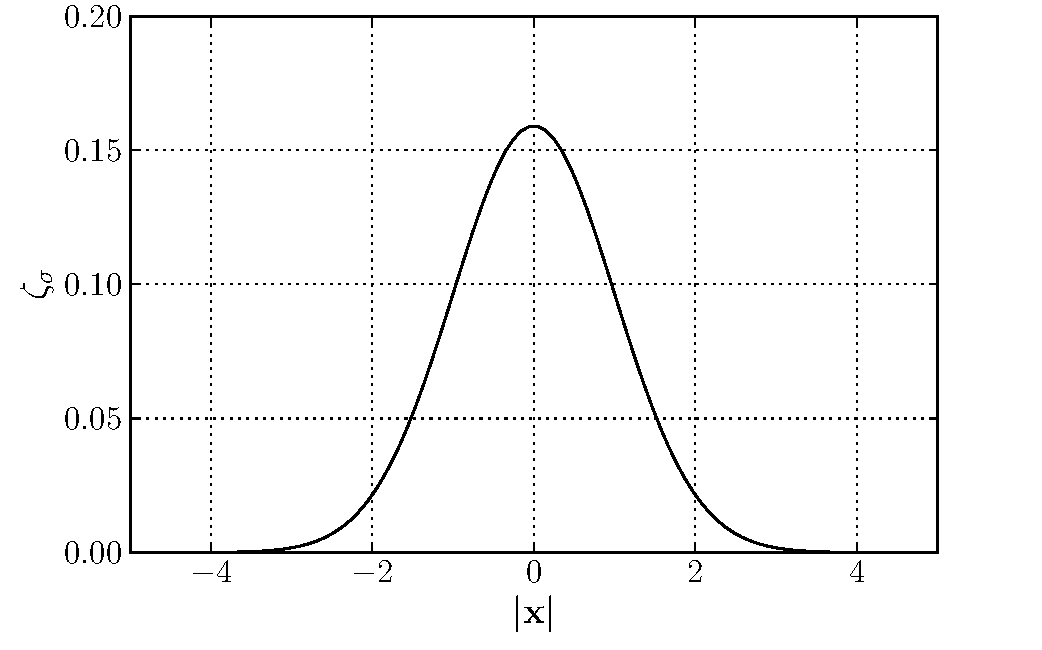
\includegraphics[width=0.6\textwidth]{figures/lagrangian/gaussianKernel.pdf}
	\caption{The smoothing function $\zeta_{\sigma}$ for a gaussian distribution with $k=2$, $\sigma=1$.}
	\label{fig:gaussianDistribution}
	\end{figure}

Figure \ref{fig:gaussianDistribution} depicts the smoothing function $\zeta_{\sigma}$ with $k=2$ and $\sigma = 1$, showing that the function decays quickly away from the center of the core. The mollified Biot-Savart kernel $\mathbf{K}_{\sigma}$ is given as,	 
	\begin{equation}
	\mathbf{K}_{\sigma} = \mathbf{K} \star \zeta_{\sigma}, 
	\end{equation}
resulting in the discrete mollified vorticity field as,
	\begin{equation}
	\omega^h\left(\mathbf{x},t\right) = \sum_p \alpha_p\left(t\right)\zeta_{\sigma}\left[\mathbf{x}-\mathbf{x}_p\left(t\right)\right],
	\label{eq:mollifiedVorticityField}
	\end{equation}
and the discrete mollified velocity field as,
	\begin{equation}
	\mathbf{u}^h\left(\mathbf{x},t\right) = \sum_p \mathbf{K}_{\sigma}\left[\mathbf{x}-\mathbf{x}_p\left(t\right)\right]\alpha_p\left(t\right).
	\label{eq:mollifiedVelocityField}	
	\end{equation}

Koumoutsakos and Chorin \cite{Cottet2000a}, explained that in order to ensure the smoothness of the velocity field, the vortex blobs need to have an overlap with each other. The overlap ratio $\lambda$ is defined as,
	\begin{equation}
	\lambda = \frac{h}{\sigma},
	\label{eq:overlapRatio}
	\end{equation}
where $h$ is the nominal particle spacing, and $\sigma$ is the vortex blob core size. Figure \ref{fig:blobOverlap} shows the visual representation of this definition. 

The overlap constraint is violated during the convection of the vortex blobs. Due to the strains in the flow, the vortex blobs cluster together at certain regions and disperse at others. This localized clustering effect is seen as a Lagrangian grid distortion, which is dealt with using a remeshing technique, section \ref{subsec:remeshing}.

	\begin{figure}[!t]
	\centering
	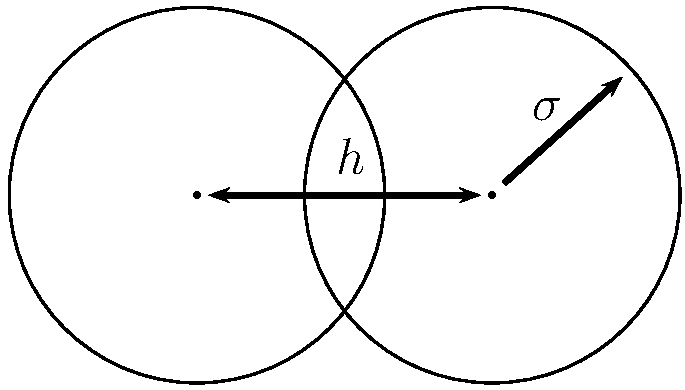
\includegraphics[width=0.4\textwidth]{figures/lagrangian/blobOverlap.pdf}
	\caption{Vortex blob with an overlap ratio $\lambda = h/\sigma$}
	\label{fig:blobOverlap}
	\end{figure}

\subsection{Vortex blob initialization}
\label{subsec:vortexBlobInitialization}
Now the question arises on how should we initialize the particle's circulation strengths $\alpha_p$ of equation 	\ref{eq:mollifiedVorticityField}. The common approach, that is used as a standard, is to estimate the particles strength by quadrature,
	\begin{equation}
	\alpha_p = \omega_p\cdot h^2,
	\label{eq:particleCirculationAssignment}
	\end{equation}

	\begin{figure}[!b]
	\centering
	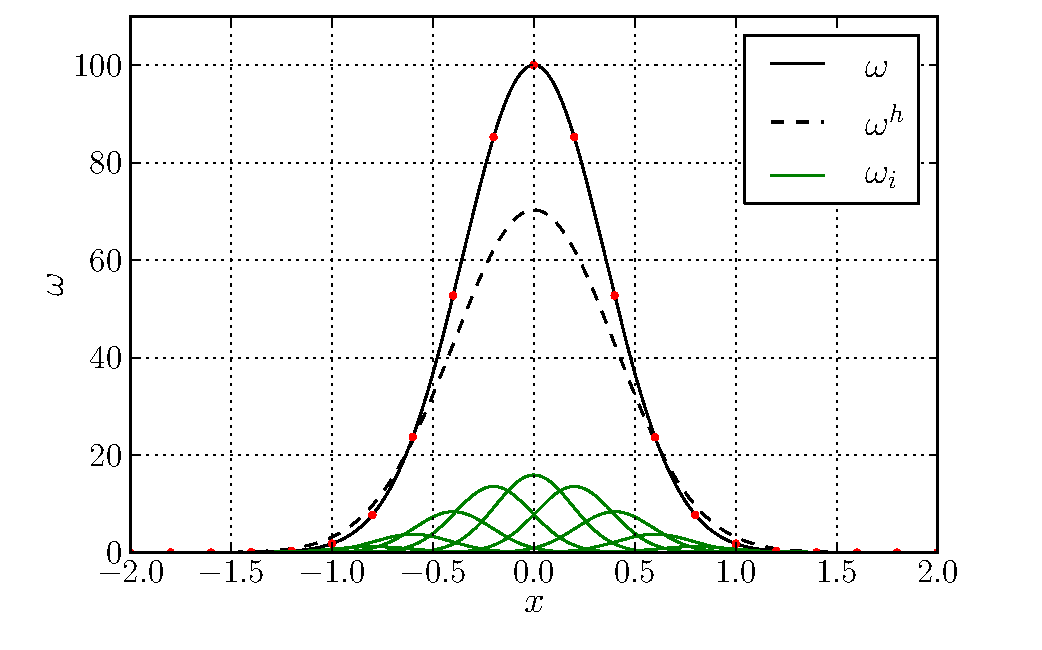
\includegraphics[width=0.6\textwidth]{figures/lagrangian/particleInitialization.pdf}
	\caption{Mollified vorticity field of a Gaussian vorticity distribution by blobs with $\lambda=1.0$, $\sigma=0.19$, and $h=0.19$. Vortex blob strengths were assigned using equation \ref{eq:particleCirculationAssignment}, sampling the exact vorticity [{\color{plotRed}{$\bullet$}}, {\color{plotRed}{\textbf{red}}} dot]. Figure depicts the exact vorticity distribution $\omega$ [---, solid \textbf{black}], the vorticity distribution of each blob $\omega_i$ [{\color{darkgreen}{---}}, solid {\color{plotGreen}{\textbf{green}}}], and the mollified vorticity field from the blobs $\omega^h$ [- -, dashed \textbf{black}].  }
	\label{fig:particleInitialization}
	\end{figure}

meaning that the particle carries the circulation of its local area. This might seem like a valid assumption as the circulation of a given area is the integral of the vorticity in the area, given by equation\ \ref{eq:definitionOfCirculation}, and therefore we will be conserving the circulation as all the circulation in the fluid is represented by the blobs.

Figure \ref{fig:particleInitialization} shows the initialization of the vorticity field using the equation 	\ref{eq:particleCirculationAssignment}. We observed that the mollified vorticity field $\omega^h$, deviates from the original intended vorticity distribution $\omega$. Barba and Rossi \cite{Barba2010a}, have described this problem as Gaussian blurring of the original vorticity field due to use of mollified vortex kernel $\zeta_{\sigma}$ in equation 	\ref{eq:mollifiedVorticityField}. Even though the total circulation is conserved, locally we see that the circulation is not conserved. 

This phenomenon causes issue during the coupling of the Lagrangian method and the Eulerian method, as particle in the overlap region are re-initialized at every step of the hybrid method. This error in initialization posses a challenge in the coupling of the method and is described in section \ref{subsec:hy_iwtca}.

A typical strategy for recovering the intended distribution is the Beale's Iterative Method \cite{Beale1988}, as used by Koumoutsakos and Cottet \cite{Cottet2000a}. The method is particle circulation processing scheme where the circulation $\alpha_p$ of the particles are modified iteratively such that the mollified vorticity field $\omega^h$ matches the original distribution $\omega$. However, the Beale's method required the correction of complete vorticity field in fluid domain and cannot be used to correct only part of the fluid domain, as required for our decomposed domain method. Therefore, an alternate method is required to minimized the error in particle initialization.

%################# Beale's Iterative method, removed.
\begin{comment}
Another way of viewing this phenomenon is to say that the conservation of circulation is only valid globally (for an infinite domain), but once we try to conserve circulation locally (e.g. in a given sub-domain), is does not satisfy anymore. Figure \ref{fig:particleInitialization} shows this effect for a simple gaussian initial vorticity distribution $\omega$. The mollified vorticity field is given as $\omega^h$ and even though the integral of both function is the same (conservation of circulation is satisfied), the vorticity functions do not match. This is does not cause a lot of issues when we only dealing with vortex particle method, however once we start using domain decomposition methods, this problem is an issue. As the vorticity is the communication between both methods, we must have accurate vorticity distribution.

A common strategy, used by Koumoutsakos, Cottet, and other for recovering the initial vorticity field is to perform the Beale's method \cite{Beale1988} \cite{Cottet2000a}.


\subsubsection*{Beale's Iterative Method}
\label{subsubsec:BealesMethod}
The Beale's method is particle circulation processing scheme where the circulation of the particles are modified such that the mollified vorticity field matches the indented vorticity field (the initial vorticity field). The recovery of the vorticity field is done by performing a discrete deconvolution,
	\begin{equation}
	\sum_j^N \beta_j \zeta_{\sigma}\left(\mathbf{x}_i-\mathbf{x}_j\right) = \omega_i,
		\end{equation}
where $\beta_j$ is the circulation of the particles at positions $\mathbf{x}_j$ such that it matches the exact vorticity $\omega_i$ at the position $\mathbf{x}_i$ that we are evaluating.  As we are try to solve for a $N$ unknown problem, we must set up an $N$ system of equations. Multiplying both sides with the area associated to the blobs, we get
	\begin{equation}
	\mathbf{A}_{ij} \beta_j = \alpha_i^{\mathrm{exact}},
	\end{equation}
where
	\begin{equation}
	\mathbf{A}_{ij} = \zeta_{\sigma}\left(\mathbf{x}_i - \mathbf{x}_j\right) \cdot h^2.
	\end{equation}

This is an $N \times N$ matrix containing the weights of the influence of each particle on each other. When we are dealing with large number of vortex blobs, we see that it is very expensive to invert the matrix $\mathbf{A}$, meaning that we would have to use a more efficient method. Furthermore as the deconvolution problem is a severely ill-condition problem \cite{Cottet2000a}, we should not directly invert the matrix. Beale's proposition to this problem was to iteratively solve for the solution,
	\begin{equation}
	\beta_{j}^{n+1} = \alpha_i + \beta_i^n - \mathbf{A}_{ij}\cdot\beta_j^n
	\end{equation}
	
We see that with just two iterations, the error between the mollified and exact vorticity field reduces drastically, figure \ref{fig:bealesCorrection}. Koumoutsakos and Cottet \cite{Cottet2000a}, had shown that there was a drastic improvement in the velocity with just two to three iterations. However, the average vorticity of the blobs cell $\tilde{\omega} = \beta/h^2$ (red dot in figure \ref{fig:bealesCorrection}), is more peaky and no longer matches the initial vorticity distribution. This means that if we try to fix the mollified vorticity distribution to match the correct initial vorticity distribution, we corrupt the local circulation even more.

The another downside of using the Beale's correction method that it is only valid for an infinite domain as it performs a discrete deconvolution of a gaussian kernel with an infinite span. Therefore it applies to all of the fluid domain, meaning that if we are dealing with a decomposed domain with finite bounds, the Beale's correction cannot be used and would result in spurious results. So the Beale's correction can and should only be used for correcting the vorticity field of the whole fluid domain.

	\begin{figure}[t]
	\centering
	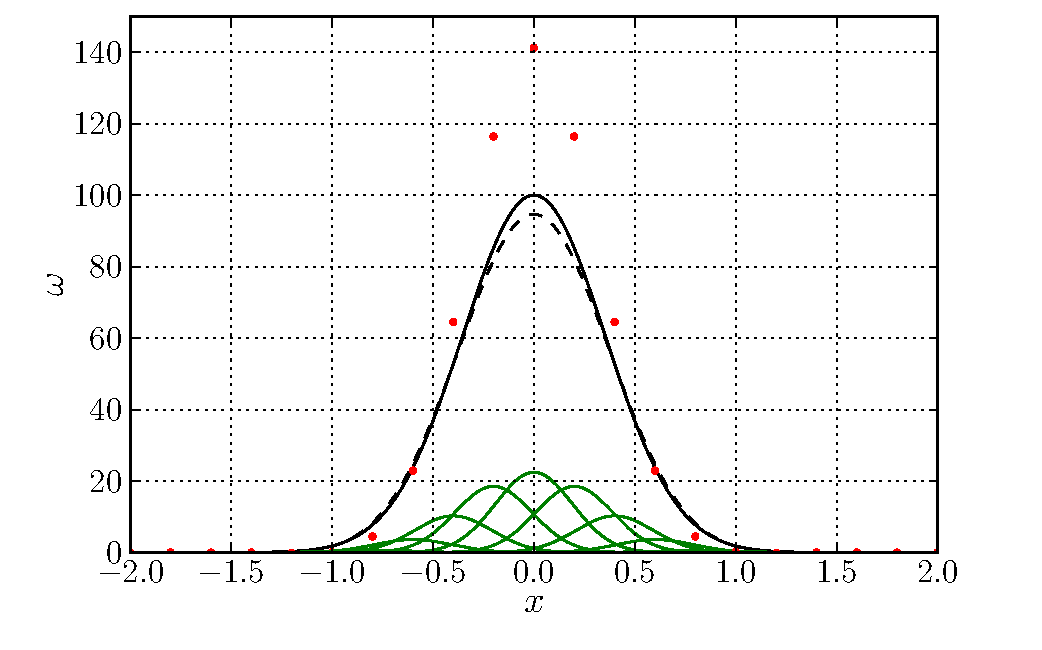
\includegraphics[width=0.7\textwidth]{figures/lagrangian/bealesCorrection.pdf}
	\caption{Mollified vorticity field after two Beale's iteration, with $\mathrm{overlap}=1.0$, $\sigma=0.19$, $h=0.19$. Figure depicts exact vorticity distribution $\omega$ [---, solid black], vorticity distribution of each blob $\omega_i$ [{\color{plotGreen}{---}}, dashed green], the mollified vorticity field $\omega^h$ [- -, dashed black], and the corrected blob cell vorticity $\tilde{\omega}=\beta/h^2$ [{\color{plotRed}{$\bullet$}}, red dot].}
	\label{fig:bealesCorrection}
	\end{figure}
\end{comment}


\subsection{Minimization of particle discretization error}
\label{subsubsec:convergenceInterpolation}
An alternate method to reduce the Gaussian blurring of the vorticity field is to modify the overlap ratio $\lambda$, and the nominal particle spacing $h$. This approach does not remove the Gaussian blurring problem, but instead minimizes its discretization error.
	
\begin{figure}[!b]
        \centering
        \begin{subfigure}[b]{0.5\textwidth}
                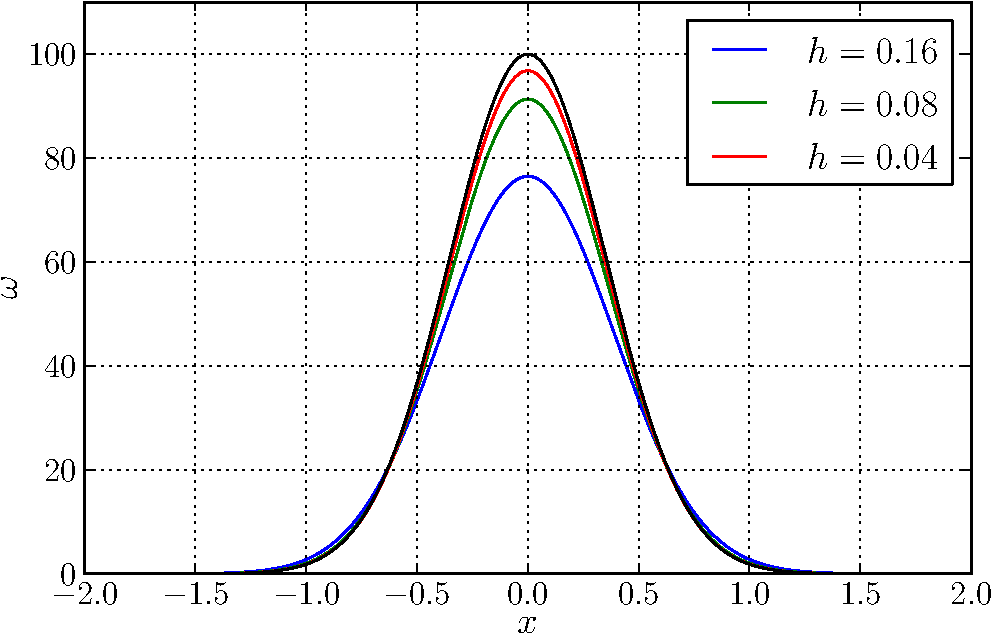
\includegraphics[width=\textwidth]{figures/lagrangian/betterInitialization_h-crop.pdf}
                \caption{Convergence of $h$ with $\lambda = 1.0$}
                \label{fig:convergenceOfBlobsH}
        \end{subfigure}%
        ~ %add desired spacing between images, e. g. ~, \quad, \qquad etc.
          %(or a blank line to force the subfigure onto a new line)
        \begin{subfigure}[b]{0.5\textwidth}
                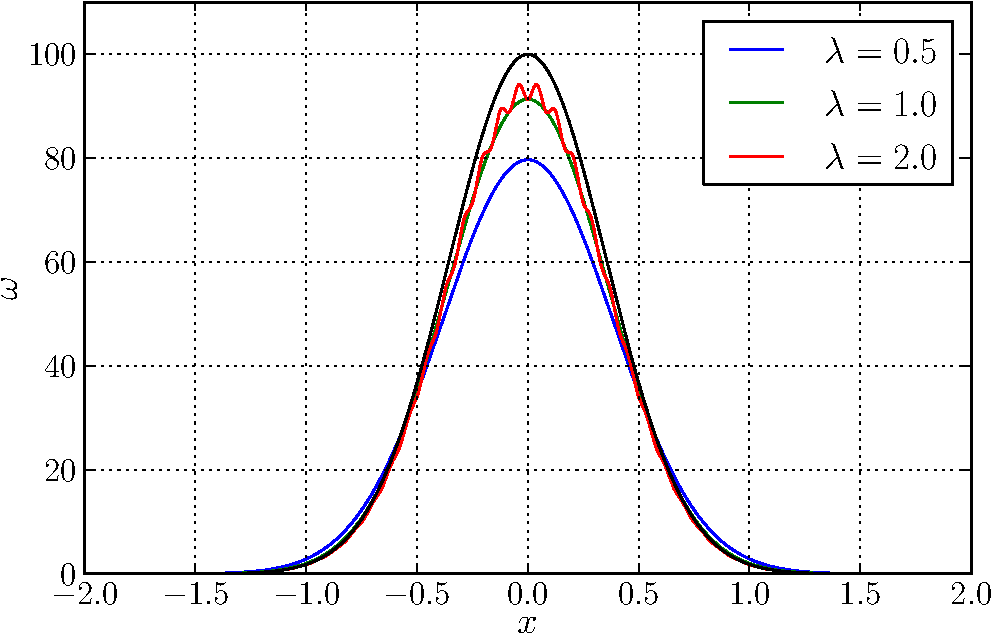
\includegraphics[width=\textwidth]{figures/lagrangian/betterInitialization_overlap_cor-crop.pdf}
                \caption{Convergence of $\lambda$ with $h = 0.08$}
                \label{fig:convergenceOfBlobsOverlap}
        \end{subfigure}
        \caption{Convergence of the spatial discretization $h$ and $\lambda$ of the initial vorticity distribution. Figure depicts the exact vorticity field $\omega$ [---, solid \textbf{black}], and various discretized vorticity distributions.}
        \label{fig:convergenceOfSpatialResolution}
\end{figure}	

Figure \ref{fig:convergenceOfSpatialResolution} shows mollified vorticity field results from modifying the spatial resolution parameters. Figure \ref{fig:convergenceOfBlobsH} shows the convergence of the mollified vorticity field $\omega^h$ to the exact vorticity field $\omega$ by reducing the nominal particle spacing $h$. The overlap ratio is set to $\mathrm{overlap} = 1$, meaning that the blob core-size $\sigma$ is equal to $h$. We see that by reducing blob core size, and simultaneously increasing the number of particles, the mollified vorticity converges to the exact vorticity. 

The second parameter we can adjust is the $\mathrm{overlap}$ of the blobs, as seen in figure \ref{fig:convergenceOfBlobsOverlap}. The blob spacing $h$ is set to $h = 0.08$, and we see that by increasing the overlap ratio $\lambda$, the mollified vorticity approaches the exact vorticity field. However, as shown by Koumoutsakos and Cottett \cite{Cottet2000a}, if the overlap is low, we lose the smooth reconstruction of the vorticity field. This can be seen for $\mathrm{\lambda} = 2.0$. We see that the mollified vorticity field has a fluctuating solution, and will result in non-smooth velocity field.

Thus, to minimize the error in initializing the mollified vorticity $\omega^h$ from the vorticity $\omega$, an overlap ratio of $\lambda = 1.0$, and a small nominal blob spacing $h$ is required. In our hybrid method, this means that at the region where we initialize the vortex blobs (i.e inside the Eulerian domain), we require these conditions to be satisfied. 

\section{Convection in Vortex Particle Method}
\label{sec:covb}

Convection of the vorticity is the first step of evolution of the vorticity from viscous splitting algorithm, from section \ref{subsec:vsa}. The convection of the vorticity is described by the first order hyperbolic equation, equation \ref{eq:convectionEulerian}. The convection equation \ref{eq:convectionEulerian}, is solved by the following system of ordinary differential equations,
	\begin{subequations}
	\begin{align}
	\frac{\mathrm{d}\mathbf{x}_p}{\mathrm{d}t} &= \mathbf{u}\left(\mathbf{x}_p\right),\\
	\frac{\mathrm{d}\alpha_p}{\mathrm{d}t} &= 0,
	\end{align}
	\label{eq:convectionODE}
	\end{subequations}
where the change in position of vortex blob $\mathbf{x}_p$ is due to the induction velocity $\mathbf{u}\left(\mathbf{x}_p\right)$ acting on it, and the strengths of the particles $\alpha_p$ is conserved.

The Biot-Savart Law, equation \ref{eq:mollifiedVelocityField}, is used to determine the induced velocities acting on each particle, resulting in an $N$-body problem. The calculation of the $N$-body problem is optimized by parallelizing the calculations in GPU hardware. The calculation is further optimized by using a fast summation method, the \printAcron{Fast Multipole Method}{FMM}, reducing the problem from $\mathcal{O}(N^2)$ to $\mathcal{O}(N)$ (in the ideal case).

The time integration of equation \ref{eq:convectionODE} is performed using a $4^{\mathrm{th}}$ order explicit Runge-Kutta method. The higher-order time integration ensures an accurate convection of the vortex blobs, resulting in minimum dissipation. However, the downside to employing a multi-stage method is that we require multiple evaluation of the induced velocity $\mathbf{u}\left(\mathbf{x}_p\right)$, when stepping from a given time $t_n$ to the next time $t_{n+1}$.

After several steps of the convection of the vortex blobs, the overlap ratio $\lambda$ will no longer be satisfied due to strains in the fluid, as described by Koumoutsakos and Chorin \cite{Cottet2000a}. In section \ref{subsubsec:convergenceInterpolation}, we determined that to have an accurate reconstruction of the vorticity field, the vortex blobs must satisfy the overlap ratio $\lambda$ at all times $t$. This introduced the need for a remeshing (or a regridding) scheme that can reconstruct the vortex blobs distribution to the original overlap ratio $\lambda$.

\subsection{Remeshing scheme: Treating lagrangian grid distortion}
\label{subsec:remeshing}

The distortion of the Lagrangian grid is due to the clustering and dispersion of the vortex blobs. This clustering and dispersing effect of the blobs is due to the high strains in the flow. Figure \ref{fig:distortion} depicts the distortion of the Lagrangian grid after 100 convection steps. The final distribution shows gaps in vortex blob distribution and will result in an inaccurate representation of the vorticity field. 

	\begin{figure}[!h]
	\centering
	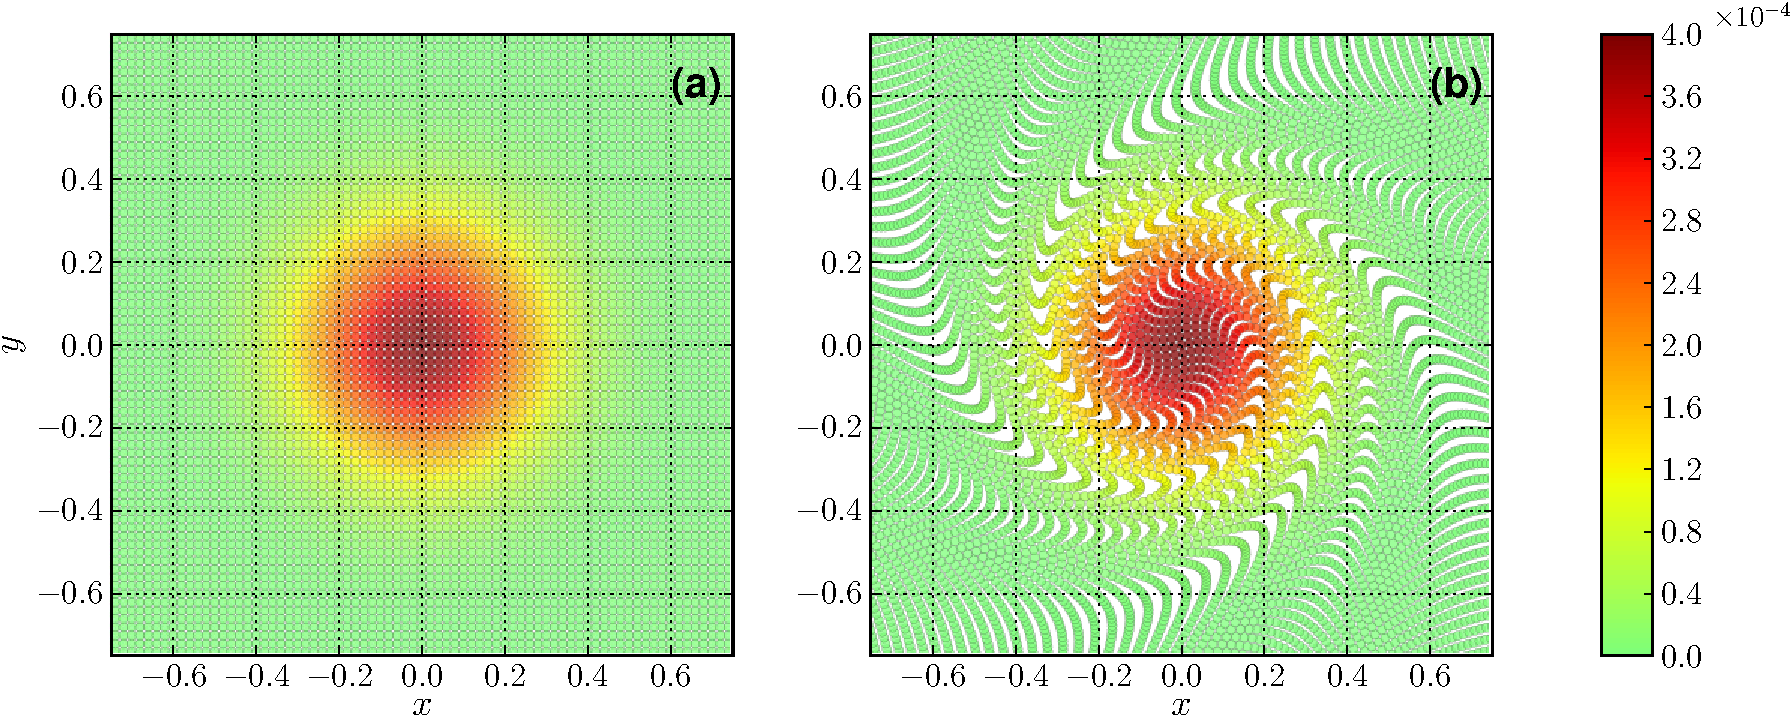
\includegraphics[width=0.9\textwidth]{figures/lagrangian/distortion-crop.pdf}
    \caption{Lagrangian distortion of the vortex blobs after 100 time steps. The initial vorticity field is $\omega\left(\mathbf{x},0\right) = \exp\left(-12\left|\mathbf{x}\right|\right)$ with $\Delta t = 0.1$, $\sigma=0.02$, and $\mathrm{overlap} = 1.0$. Figure depicts $\textbf{(a)}$ the initial distribution of the vortex blobs, and $\textbf{(b)}$ the final distribution of the vortex blobs after 100 time steps.}
    \label{fig:distortion}
	\end{figure}

	\begin{figure}[!b]
	\centering
	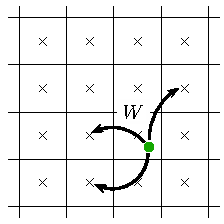
\includegraphics[width=0.4\textwidth]{figures/lagrangian/interpolationGrid.pdf}
	\caption{Remeshing of a single vortex blob [{\color{plotGreen}{$\bullet$}}, green dot] onto a uniform grid defined by the $\left(3\times3\right)$ 2-D stencil.}
	\label{fig:interpolationGrid}
	\end{figure}

A remeshing (or regridding) of this field is therefore required to retain proper distribution. It is done by interpolating the strengths of the vortex blobs from the distorted Lagrangian grid $\hat{\mathbf{x}}$ onto a uniform grid $\mathbf{x}$. The strengths of the blobs of the new uniform grid $\alpha_p$ is determined by,
	\begin{equation}
	\alpha_p = \sum_q\tilde{\alpha}_q W \left(\frac{x_p - \tilde{x}_q}{h}\right),
	\label{eq:la_remeshingKernel}
	\end{equation}
where the strengths of the blobs $\tilde{\alpha}_q$ of the distorted Lagrangian grid $\tilde{x}_q$ are transfered to the regular Lagrangian grid $x_p$ using the interpolation kernel $W$. Figure \ref{fig:interpolationGrid} shows an example of the remeshing of one vortex blob of the distorted grid on to the structured uniform grid with a kernel $W$ with a $3\times3$ stencil. During this transfer, we must ensure that the properties of the fluid are conserved. The interpolation kernel is constructed by ensuring that the total circulation, the linear impulse, and the angular impulse of the fluid are conserved. 

For the present work, the widely used $\mathrm{M}'_4$ interpolation kernel, such as by Koumoutsakos and Cottet \cite{Cottet2000a}, Speck \cite{Speck2011a}, and Barba \cite{Barba2004c}. The kernel is continuously differentiable ensuring conservation of total circulation, linear and angular impulse. 

\subsubsection*{$\mathbf{M}^\prime_4$ interpolation kernel}

The $\mathrm{M}^{\prime}_4$ interpolation kernel is an efficient interpolation kernel that has been used to reconstruct a smooth distribution, and was introduced by Monaghan in 1985 \cite{Monaghan1985}. For a 1D problem, the $\mathrm{M}'_4$ interpolation kernel is defined as,
	\begin{equation}
	{\mathrm{M'}_4}\left( {\xi} \right) =
	  \begin{cases}
	   {1 - \frac{{5{\xi ^2}}}{2} + \frac{{3{{\left| \xi  \right|}^3}}}{2}} & {\left| \xi \right|} < 1, \\
	   \frac{1}{2}{\left( {2 - \left| \xi  \right|} \right)^2}\left( {1 - \left| \xi  \right|} \right) & 1 \leqslant {\left| \xi \right|} < 2,\\
	   0 & 2 \leqslant \left| \xi \right|,
	  \end{cases}
	\label{eq:interpKernel}
	\end{equation}
where
	\begin{equation}
	\xi = \frac{x_{\nu} - x_i}{h},
	\label{eq:xiEquation}
	\end{equation}
	
is a non-dimensional parameter, relating the position of the particle $x_{\nu}$ to the position of the $i^{\mathrm{th}}$ interpolation node $x_i$. The $\mathrm{M'}_4$ is a third-order accurate, piecewise smooth, B-spline kernel. The kernel with the $m = 4$, has a 4 support nodes in each dimension. 

	\begin{figure}[!h]
	\centering
	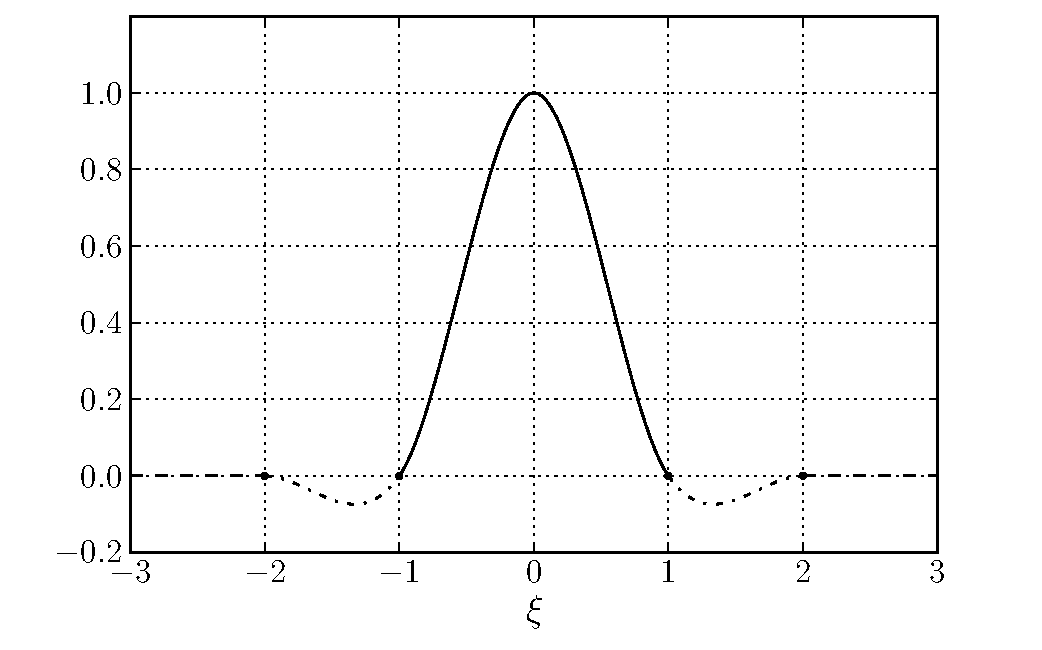
\includegraphics[width=0.6\textwidth]{figures/lagrangian/interpolationKernel.pdf}
	\caption{$M'_4$ interpolation kernel, a third-order, piecewise smooth, B-spline kernel by Monaghan \cite{Monaghan1985}}
	\label{fig:interpolationKernel}
	\end{figure}

Figure \ref{fig:interpolationKernel} shows the distribution of the kernel. For the 2D problem, the 2D interpolation kernel is the tensor product of the 1D interpolation kernel, thus having a $4\time4 = 16$ support nodes. The kernel has a compact support, making it ideal for an efficient $\mathcal{O}(N)$ remeshing.

%Koumoutsakos \cite{Koumoutsakos1997} has investigated the drawback of the employing the remeshing strategy and have shown that there is approximately $4\%$ decay in enstrophy of the flow due to sub-grid dissipation. Note that enstrophy $ \mathcal{E}$, is defined as
%
%% 4 % , give context, what time, how many remshings, say they are negligible for what we do.
%
%	\begin{equation}
%	\mathcal{E} = \frac{1}{2}\int_S \omega^2 dS
%	\end{equation}
%	
%and is directly related to the kinetic energy of the fluid and gives and insight in the energy production and the dissipation of the fluid. Enstrophy is especially useful in turbulence flow investigation as it helps describe the energy cascade of the fluid.		

\section{Diffusion in Vortex Particle Method}
\label{sec:diffusionVM}

Chorin \cite{Chorin1973a}, simulated the viscous flow using the viscous splitting algorithm, described in section \ref{subsec:vsa}. The viscous splitting algorithm segregated the vorticity transport equation, equation \ref{eq:la_vteq}, to the inviscid and the viscous components, equation \ref{eq:convectionEulerian} and equation \ref{eq:vsa2} respectively. 

The flow is convected during the first sub-step, whereas in the second sub-step, we have to deal with the diffusion of the vorticity field, equation \ref{eq:vsa2}. The diffusion problem is solved using the following system of ODEs, 
	\begin{subequations}
	\begin{align}
	\frac{\mathrm{d}\mathbf{x}_p}{\mathrm{d}t} &= 0,\\
	\frac{\mathrm{d}\alpha_p}{\mathrm{d}t} &= \nu\Delta\alpha_p,
	\end{align}
	\label{eq:la_sysODEsDiff}
	\end{subequations}
where the position of the particles $\mathbf{x}_p$ is fixed, whereas the change in strengths of the particles $\alpha_p$ as depended on the kinematic viscous $\nu$. Thus the diffusion of the vortex blobs requires only the modification to the strengths $\alpha_p$ of the particles. 

Chorin in 1973 \cite{Chorin1973a}, initially employed the \indexAcron{Random Walk Method}{RWM}, which generates and disperses vorticity using a pseudo-random number algorithm. However, this method suffered some limitations in accuracy, and since then methods such as \indexAcron{Particle Strength Exchange}{PSE} method \cite{Degond1989a}, and \printAcron{Vortex Redistribution Method}{VRM} \cite{Shankar1996} become a popular choice for treating diffusion of the particles.

The VRM simulates the diffusion of the particles by redistributing fractions of circulations of the vortex blobs to each other, such that diffusion is appropriately modeled. These redistribution fractions $f_{ij}^n$ are determined by solving a linear system of equations, that conserves the moments of the particles (such as the total circulation, linear and angular impulse) and the diffusion of the flow. 

The redistribution fractions $f_{ij}^n$, transfers portion of circulation $\alpha_p$ of the particle $p$ to others within the diffusion radius, defined as,
	\begin{equation}
	h_{\nu} = \sqrt{\nu\Delta t_d}
	\label{eq:la_diffDis}
	\end{equation}
where $h_{\nu}$ is the diffusion distance and is directly related to the kinematic viscosity $\nu$ and the diffusive time step size $\Delta t_d$ of the simulation.

For this work, we investigate two methods that employ this approach. The Wee-Ghoniem Remeshing Scheme \cite{Wee2006a} implemented the VRM into the remeshing process, section \ref{subsec:modifiedRemeshing}. The advantage was that diffusion and remeshing can be performed simultaneously in a single process. However for some flow cases, this approach had undesirable constraint on the diffusion time step size $\Delta t_d$. Therefore, the approach of Tutty \cite{Tutty2010a}, the Tutty Remeshing Scheme, was employed which had a desirable constraint on the diffusion time step size $\Delta t_d$, section \ref{subsubsec:srs}. The scheme was used to perform diffusion at every step of the evolution, which is important for proper coupling of the Eulerian and the Lagrangian method.

%This means that the VRM scheme (and also the PSE) requires a search algorithm to determine the particles that are within the zone of influence. A direct evaluation would require an $\mathcal{O}\left(N^2\right)$ evaluation. However, this can be optimized using a search tree algorithm, speeding up the search to an $\mathcal{O}\left(\log N\right)$.

%Not that the diffusive time-step $\Delta t_d$ is equal to the convective time-step $\Delta t_c$ if the diffusion process is done during every time-step. However, we can easily adjust the diffusion time-step and perform diffusion at a multiple step of the convection. Not diffusing at every step can be helpful as 

%The downside of the this approach, as also for the standard remeshing approach is the global remeshing generates large computation data and scales with the number of particles $N$. Therefore for problems with large number of particles, a tree-structured remeshing would be more feasible strategy \cite{Winckelmans1996}.


\begin{comment}
\subsubsection*{Particle Strength Exchange}
The Particle Strength Exchange method, first proposed by Mas-Gallic in 1989 \cite{Degond1989a}, showed that diffusion can be treated for a particle method with an isotropic, or an anisotropic viscosity by approximating the diffusion operator (a Laplacian) with an integral operator, and discretize the method with particles \cite{Speck2011a}. %The PSE can be seen as circulation correction method, where during the diffusion step of the viscous splitting algorithm, the strengths of the particle are corrected such that it accounts for the diffusion.
 
\subsubsection*{Vortex Redistribution Method}
An alternative method to simulate the diffusion is to use the \printAcron{Vortex Redistribution Method}{VRM} \cite{Shankar1996}. The model simulates diffusion by distributing the fraction of circulation of the vortex blobs to each other satisfying the diffusion. The model is based on conserving the moments of the particles by satisfying a linear system of equations. The circulation of the particle are transfer to the nearby particles that are,
	\begin{equation}
	h_{\nu} = \sqrt{\nu\Delta t_d}
	\end{equation}
where $h_{\nu}$ is the diffusion distance and is directly related to the kinematic viscosity $\nu$ and the diffusive time-step $\Delta t_d$ of the simulation. This means that the VRM scheme (and also the PSE) requires a search algorithm to determine the particles that are within the zone of influence. A direct evaluation would require an $\mathcal{O}\left(N^2\right)$ evaluation. However, this can be optimized using a search tree algorithm, speeding up the search to an $\mathcal{O}\left(\log N\right)$.

%Not that the diffusive time-step $\Delta t_d$ is equal to the convective time-step $\Delta t_c$ if the diffusion process is done during every time-step. However, we can easily adjust the diffusion time-step and perform diffusion at a multiple step of the convection. Not diffusing at every step can be helpful as 

%The downside of the this approach, as also for the standard remeshing approach is the global remeshing generates large computation data and scales with the number of particles $N$. Therefore for problems with large number of particles, a tree-structured remeshing would be more feasible strategy \cite{Winckelmans1996}.

\end{comment}

\subsection{Wee Remeshing Scheme}
\label{subsec:modifiedRemeshing}

Ghoniem and Wee \cite{Wee2006a}, observed the similarities between the VRM and the standard remeshing strategy described in section \ref{subsec:remeshing}. They proposed to combine the remeshing and the diffusion of the vortex blobs together in one single process. The application of this methodology was later investigated by Speck \cite{Speck2011a}. This approach, referred to as the \indexAcron{Wee-Ghoniem Remeshing Scheme}{WRS}, implements the diffusion of the vortex blobs in the interpolation kernel $W$ of equation \ref{eq:la_remeshingKernel}.

The key advantage of the WRS is that, now we are dealing with a uniform grid, and does not require a search algorithm to find the particles in the zone of influence, equation \ref{eq:la_diffDis}. This significantly reduces the computational cost, making this diffusion scheme practical for large scale simulations. 

The modified $\mathrm{M'}_4$ kernel for treating the diffusion is given as,
	\begin{equation}
	{{{\rm{M'}}}_4}\left( {\xi ,c} \right) =
	  \begin{cases}
	   {1 - \frac{{5{\xi ^2}}}{2} + \frac{{3{{\left| \xi  \right|}^3}}}{2} - {c^2}\left( {2 - 9{\xi ^2} + 6{{\left| \xi  \right|}^3}} \right)} & {\left| \xi \right|} < 1, \\
	   \frac{1}{2}{\left( {2 - \left| \xi  \right|} \right)^2}\left( {1 - \left| \xi  \right|} \right) - {c^2}{\left( {2 - \left| \xi  \right|} \right)^2}\left( {1 - 2\left| \xi  \right|} \right) & 1 \leqslant {\left| \xi \right|} < 2,\\
	   0 & 2 \leqslant \left| \xi \right|,
	  \end{cases}
	\label{eq:modInterpKernel}
	\end{equation}
where 
	\begin{equation}
	c^2 = \frac{\nu \Delta t_d}{h^2},
	\label{eq:c2}
	\end{equation}
is a non-dimensional number that corresponds to the transfer weight for the diffusion. The constant $c^2$ is a function of the kinematic viscosity $\nu$, diffusion time step size $\Delta t_d$ and the remeshing grid spacing $h$. This additional term in the interpolation kernel accounts for the diffusion process. When $c \rightarrow 0$, the interpolation kernel simply turns into the standard remeshing kernel, equation \ref{eq:interpKernel}. 

Ghoniem and Wee also investigated the error growth and the stability properties of the interpolation kernel in the Fourier space and have determined that for a stable diffusion and remeshing, the following constraint has to be satisfied,
	\begin{equation}
	\frac{1}{6} \leqslant c^2 \leqslant \frac{1}{2}.
	\label{eq:c2stability}
	\end{equation}

%to minimize the error growth amplification factor and the phase error. With this, we will ensure the stability of the problem and suppress any spurious oscillations and ensure that it is a non-negative interpolation kernel with non-negative redistribution fractions. 
However, we see that this $c^2$ constraint imposes a direct constraint not only on the maximum diffusion time step size $\Delta t_d$, but also imposes a constraint on the minimum step size. This would mean that the diffusion time step size $\Delta t_d$ will be sometimes larger than the convection step $\Delta t_c$,
	\begin{equation}
	\Delta t_d = k_d \cdot \Delta t_c.
	\label{eq:la_dtcts}
	\end{equation}

where $k_d \geqslant 1$ and is an integer. This is a problem for the hybrid method as the Lagrangian method and the Eulerian method are coupled at every step. If the Lagrangian method does not perform diffusion at every step, from the Eulerian method's point of view, it would seem that the Lagrangian vorticity diffuses in a discontinuous fashion. This discontinuous behavior of the Lagrangian method (w.r.t. the Eulerian method), can cause stability issues during the coupling process, and therefore should be avoided.

We could minimize this problem by modifying the $\Delta t_c$ such that it matches the diffusion time step (i.e $\Delta t_c = \Delta t_d$), so that the diffusion is performed at every step. This was a feasible solution for low Reynolds number flows, however for high Reynolds number $Re$ flows, where the convection time step has to be small, we need a scheme that is not constrained by the minimum diffusion time step.

\subsection{Tutty Remeshing Scheme}
\label{subsubsec:srs}

The \printAcron{Tutty Remeshing Scheme}{TRS}, developed by Tutty in 2010 \cite{Tutty2010a}, was based on the VRM of Shankar and Van Dommelen \cite{Shankar1996}. The scheme it possible to remesh and diffuse the vorticity after every convection step. The strengths of the particles after the remeshing and diffusion $\alpha_i^{n+1}$, are given as, 
	\begin{equation}
	\alpha_i^{n+1} = \sum_k \alpha_k^n W_{ki}^n, 
	\end{equation}
where $W_{ki}^n$ is the fraction of circulation transferred from vortex blob $k$ (old) to the new vortex blob $i$ (new), figure \ref{fig:interpolationGrid}. Tutty \cite{Tutty2010a}, explained that the fractions $W_{ki}^n$ are calculated by imposing a conservation of vorticity, center of vorticity, linear, and angular momentum of the vortex blobs, given as,
	\begin{subequations}
	\begin{align}
	\sum_k W_{ki}^n &= 1, \\
	\sum_k W_{ki}^n(x_i - x_k) = \sum_k W_{ki}^n(y_i - y_k) &= 0, \\
	\sum_k W_{ki}^n(x_i - x_k)^2 = \sum_k W_{ki}^n(y_i - y_k)^2 &= 2h_{\nu}^2, \\
	\sum_k W_{ki}^n(x_i - x_k)(y_i - y_k) &= 0,	
	\end{align}
	\label{eq:la_VRMredistributions}
	\end{subequations}
where $h_{\nu}$ is the characteristic diffusion distance associated to the time $\Delta t_d$, 
	\begin{equation}
	h_{\nu} = \sqrt{\Delta t_d \cdot \nu}.
	\end{equation}	

	\begin{figure}[!b]
	\centering
	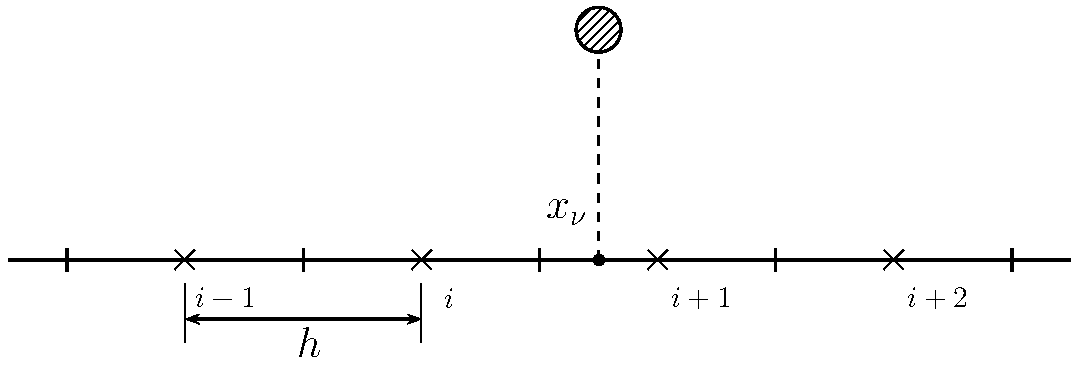
\includegraphics[width=0.7\textwidth]{figures/lagrangian/simpleRedistribution.pdf}
	\caption{1D \printAcron{Tutty Remeshing Scheme}{TRS}, diffusing the vortex blobs at $x_i \leqslant x_{\nu} \leqslant x_{i+1}$, onto the four stencil points $k=i-1,\dots,i+2$, with a grid spacing $h$.}
	\label{fig:simpleRedistribution}
	\end{figure}
	
Similar to the the TRS, described in section \ref{subsec:modifiedRemeshing}, the TRS transfers the strengths to known set of new nodes rather than the neighboring nodes (removing the requirement for a search algorithm). Figure \ref{fig:simpleRedistribution} shows the 1D redistribution of the vortex blob $x_i \leqslant x_{\nu} \leqslant x_{n+1}$ to the stencil nodes $x_k$, where $k=i-1,\cdots,i+2$. The solution to the redistribution is given by the following equations,
	\begin{subequations}
	\begin{align}
	f_{i-1} &= \frac{1}{2}\left(1-f_i-\Delta\right)\\
	f_i &= 1 - 2\left(\frac{h_{\nu}}{h}\right)^2 - \Delta^2\\
	f_{i+1} &= \frac{1}{2}\left(1-f_i+\Delta\right)\\
	f_{i+2} &= 0
	\end{align}
	\end{subequations}
and 	
	\begin{subequations}
	\begin{align}
	g_{i-1} &= 0\\
	g_{i} &= \frac{1}{2}\left(1-g_{i+1}-\Delta_1\right)\\
	g_{i+1} &= 1 - 2\left(\frac{h_{\nu}}{h}\right)^2 - \Delta_1^2\\
	g_{i+2} &= \frac{1}{2}\left(1-g_{i+1}+\Delta_1\right)
	\end{align}
	\end{subequations}
where $\Delta$ is defined as,
	\begin{equation}
	\Delta = \frac{x_{\nu}-x_i}{h},
	\end{equation}
as depicted in figure \ref{fig:simpleRedistribution}. Note that $\xi_1 = \xi - 1$. The total redistribution fractions $F_k$, are the linear combinations of the functions $f_k$ and $g_k$,
	\begin{equation}
	F_k = \left(1-\Delta\right)\cdot f_k + \Delta\cdot g_k, \quad k = i-1,\dots,i+2,
	\end{equation}

For the 2D, the redistribution fractions are simple tensors product of the $x$ and $y$ 1D redistribution fractions,
	\begin{equation}
	W_{kl} = F_k G_l, \quad k = i-1,\cdots,i+2, \quad \l = j-1,\dots,j+2,
	\end{equation}
with a 16 point stencil when $\xi=1/2$.

The stability of the redistribution requires a positive redistribution fraction, $W_{kl}^n > 0$, imposing a direct constraint on the diffusive distance,
	\begin{equation}
	\frac{h_{\nu}}{h} < \frac{1}{\sqrt{2}}.
	\end{equation}
as explained by Tutty \cite{Tutty2010a}. A resulting constraint is imposed on the maximum diffusion time step size $\Delta t_d$,
	\begin{equation}
	\Delta t_d < \frac{h^2}{2\nu}.
	\label{eq:TRS_difftimeconstr}
	\end{equation}

Therefore, we observe that this scheme only poses a constraint on the maximum diffusion time step size $\Delta t_d$, enabling us to perform the diffusion at every step of the evolution, equation \ref{eq:la_dtcts}.

When employing the Tutty's scheme, we require diffusion and redistribution to be performed at every step, i.e the diffusion frequency $f_{diff}=1$ and the redistribution frequency $f_{redis}=1$. In addition to the redistribution, a common approach to minimize the number of vortex blobs is to perform a population control. A population control removes particles with strengths $\left|\alpha\right|$ less than pre-defined circulation threshold $\Gamma_{loc}$, and simultaneously ensuring that the total circulation removed is less that the pre-defined global threshold $\Gamma_{glob}$,

\begin{equation}
\sum_i \left|\alpha_i\right| \leqslant \Gamma_{glob},
\end{equation}

where $\alpha_i$ is the strength of the removed particle $i$. Typically, the population control is performed in conjunction with the redistribution, i.e $f_{redis}=f_{pc}=1$.

%In addition to the remeshing process, we also performed a population control to minimized the number of vortex blobs. After the remeshing process, we may acquire vortex blobs that have negligible influence on other particles, due to its small particle strength. Therefore, we can remove these particles by ensuring that the circulation will be conserved. 


%The one-dimension redistribution fractions for $x$-direction is a linear combination of the two basis solution for a conservative redistribution,
%	\begin{equation}
%	F_k = \left(1-\Delta\right)\cdot f_k + \Delta\cdot g_k, \quad k = i-1,\dots,i+2,
%	\end{equation}
%having a four point stencil, as show in figure \ref{fig:simpleRedistribution}.  

%In the above equation, $h_{\nu}$ is the characteristic diffusion distance during the time $\Delta t_d$, 
%We have to note that, $f_k$ and $g_k$ is zero for all the other $k$. 
%	\begin{equation}
%	h_{\nu} = \sqrt{\Delta t_d \cdot \nu}.
%	\end{equation}
		
%The only constraint imposed for a positive redistribution fraction is,
%
%giving us the maximum time step size constraint of,
%	\begin{equation}
%	\Delta t_d < \frac{h^2}{2\nu}.
%	\end{equation}
	
%Therefore, we observe that this scheme only poses a constraint on the maximum diffusion time step size $\Delta t_d$, enabling us to perform the diffusion at every step of the evolution, equation \ref{eq:la_dtcts}.

\section{Boundary conditions for viscous Vortex Particle Method}
\label{sec:boundaryConditions}

For incompressible viscous flows, the solid boundary is the vorticity generator of the flow. So far, we have only dealt with unbounded flow. For bounded flow simulation, we must enforce the boundary condition of the flow. In 2D, the boundary condition for an immersed body, translating at velocity $\mathbf{u}_b(t)$ with an angular velocity $\Omega(t)$ about it's center of mass $\mathbf{x}_b$ is given as,
\begin{equation}
\mathbf{u}(\mathbf{x}_s) = \mathbf{u}_s
\label{eq:la_bcSlip}
\end{equation}
with,
\begin{equation}
\mathbf{u}_s = \mathbf{u}_b + \Omega(t) \times (\mathbf{x}_s - \mathbf{x}_b),
\end{equation}

where $\mathbf{u}_s$ is the velocity at the surface point $\mathbf{x}_s$. However, in the present work, we deal with stationary bodies and so $\mathbf{u}_b = 0$ and $\Omega(t) = 0$. The boundary condition, Equation \ref{eq:la_bcSlip}, is usually expressed as,
\begin{equation}
\mathbf{u} \cdot \hat{\mathbf{s}} =  \mathbf{u}_s \cdot \hat{\mathbf{s}}.
\end{equation}
equating the tangential components $\hat{\mathbf{s}}$, and is referred to as the \emph{no-slip} boundary condition. The paper of Koumoutsakos, Leonard and Pepin \cite{Koumoutsakos1994b} stated that, by satisfying no-slip boundary condition directly satisfies the no-through boundary conditions, as these boundary conditions are linked (\emph{Linked boundary condition}). This was also been stated by Shiels \cite{Shiels1998} and have been further employed by Cooper, Mar and Barba in 2009 \cite{Cooper2009a}.

	\begin{figure}[!h]
	\centering
	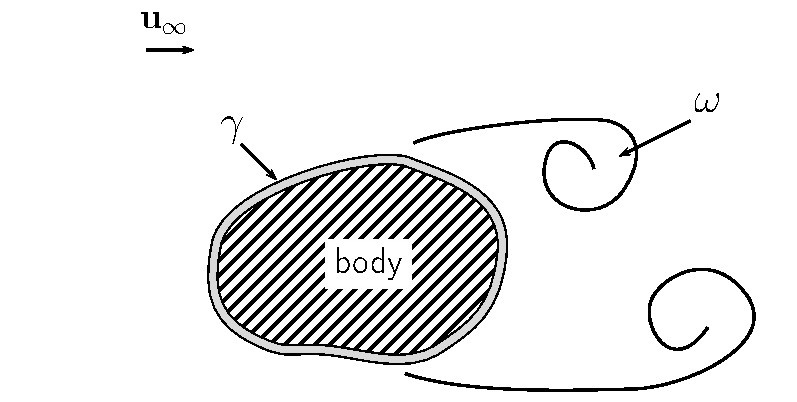
\includegraphics[width=0.6\textwidth]{figures/lagrangian/noSlipVorticityField.pdf}
	\caption{Extended vorticity field separated into vorticity in the fluid and the vortex sheet distribution confined to the body.}
	\label{fig:noSlipVorticityField}
	\end{figure}

Typically in an inviscid flow, the boundary condition is enforced after performing the Helmholtz decomposition of the velocity, equation \ref{eq:helmholtz}. The rotational component $\mathbf{u}_{\omega}$ represents the velocity due to the vorticity in the flow, whereas the potential component $\mathbf{u}_{\phi}$ is used to taken in account of the presence of the body. However, Koumoutsakos, Leonard and Pepin in 1994 \cite{Koumoutsakos1994b}, used an alternate approach for enforcing the boundary condition. Instead of performing the Helmholtz decomposition, they considered an extended vorticity field that is divided into:
\begin{itemize}
\item the vorticity field in the fluid $\omega$,
\item the vortex sheet distribution on the boundary $\gamma$,
\end{itemize}
Figure \ref{fig:noSlipVorticityField} depicts this extended vorticity and the division of the vorticity field to the two sub-categories. The resulting velocity field throughout the domain is given as,
\begin{equation}
\mathbf{u} = \mathbf{u}_{\omega} + \mathbf{u}_{\gamma} + \mathbf{u}_{\infty}
\label{eq:la_noslipbcsimple}
\end{equation}
where $\mathbf{u}_{\omega}$ is velocity field induced by the vorticity in the flow, $\mathbf{u}_{\gamma}$ is the velocity field induced by the vortex sheet and $\mathbf{u}_{\infty}$ is the free-stream velocity.

The vortex sheet distribution $\gamma$ on the boundary is defined by the boundary integral equations, which will be used to enforce the boundary condition.

% Using the Helmholtz decomposition, we can have decompose the velocity field in to the rotational and the irrotational components, equation \ref{eq:helmholtz}. We can use the potential component to prescribe the boundary conditions at the solid wall boundary,
%	\begin{equation}
%	\mathbf{u}_{\phi} = \nabla\Phi.
%	\end{equation}

%The incompressibility constraint results in a Laplace's equation for the potential field and a unique solution is %obtained by enforcing the wall boundary conditions,
%	\begin{equation}
%	\mathbf{u}_b\cdot\mathbf{\hat{n}} = \left(\mathbf{u}_{\omega} + \nabla\Phi\right) \cdot \mathbf{\hat{n}},
%	\label{eq:potentialBC}
%	\end{equation}

%enforcing the no-through flow at the solid boundary wall, moving at $\mathbf{u}_b$, where $\mathbf{\hat{n}}$ is the normal vector of the solid boundary. The approach for determine the solution to the Laplace's equation is by Green's function formulation. This approach required a singularity distribution over the body resulting in the appropriate boundary condition. Doublets and/or source panels are used to attain the required potential such that equation \ref{eq:potentialBC} is satisfied.

%\subsubsection{Linked boundary conditions}

%However Koumoutsakos, Leonard and Pepin in 1994 \cite{Koumoutsakos1994b}, suggested to use vortex sheets to enforce the boundary conditions. This alternate approach of enforcing the solid boundary condition is by not to decompose the velocity field into potential and rotational but to consider the solid boundary as an extension of the vorticity field through vortex sheets $\gamma$, figure \ref{fig:noSlipVorticityField}. Due to the non-zero tangential velocity at the surface, a sudden discontinuity in the velocity field can be considered as vortex sheet. So to enforce the boundary conditions of the solid wall, we must satisfy the no slip velocity at the boundary,
%	\begin{equation}
%	\mathbf{u}\cdot\mathbf{\hat{s}} = \mathbf{u}_b\cdot\mathbf{\hat{s}}.
%	\end{equation}

%Koumoutsakos \cite{Koumoutsakos1993b}, relied only on the vortex sheets to enforce the no-slip velocity. Koumoutsakos, Leonard and Pepin's paper in 1994 \cite{Koumoutsakos1994b} stated that, by satisfying no-slip boundary condition, it directly satisfies the no-through boundary conditions, as these boundary conditions are linked. This was also been stated by Shiels \cite{Shiels1998} and have been further employed by Cooper, Mar and Barba in 2009 \cite{Cooper2009a}. So enforcing the no-slip boundary condition directly satisfies the no-through constraint at the surface.


\subsection{Boundary integral equations}

The Lagrangian method that we are using for the hybrid scheme, is modified according to Stock \cite{Stock2010a}. The Lagrangian method under-resolved the vorticity field in the near-wall region. Furthermore, the vorticity of the fluid is segregated between the vortex blob domain and the vortex sheet domain, as seen in figure \ref{fig:extendedVorticityField}. The figure shows that, very near the wall the vorticity of the fluid is represented by the vortex sheet. In other words, the vortex sheet is an extension to the vorticity represented by the vortex blobs. %The extended velocity field (of the extended vorticity field) is summarized as,
%	\begin{equation}
%	\mathbf{u} = \mathbf{u}_{\omega} + \mathbf{u}_{\gamma} + \mathbf{u}_{\infty}
%	\end{equation}
%where the $\mathbf{u}_{\gamma}$ denotes the velocity field induced by the vortex sheet. 

Enforcing the no-slip boundary conditions, equation \ref{eq:la_noslipbcsimple}, we have that,
	\begin{equation}
	\left(\mathbf{u}_{\mathrm{ext}} + \mathbf{u}_{\gamma}\right)\cdot\mathbf{\hat{s}} = \mathbf{u}_s \cdot \mathbf{\hat{s}}
	\label{eq:kinematicBCofVSOutside}
	\end{equation}
where $\mathbf{u}_{\mathrm{ext}} = \mathbf{u}_{\omega} + \mathbf{u}_{\infty}$ is the velocity field induced from the vortex blob domain (i.e external to vortex sheet domain). The equation states that the tangential component of the total velocity acting on the body should be equal to the tangential velocity of the body. So the induced velocity of the vortex sheet is given as,
	\begin{equation}
	\left(\mathbf{u}_{\mathrm{ext}} - \mathbf{u}_s\right) \cdot \mathbf{\hat{s}} = \mathbf{u}_{\gamma}\cdot\mathbf{\hat{s}}.
	\label{eq:kinematicBCofVS}
	\end{equation}

	\begin{figure}[t]
	\centering
	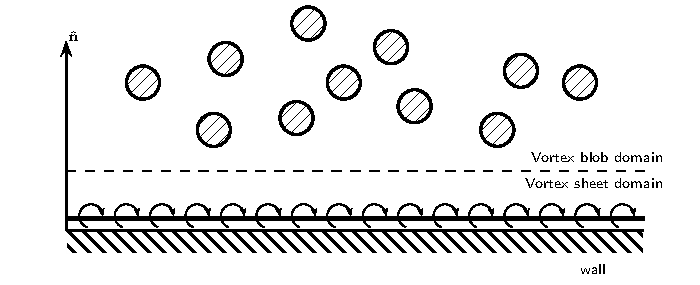
\includegraphics[width=0.8\textwidth]{figures/lagrangian/extendedVorticityField.pdf}
	\caption{Extended vorticity field: Vortex sheet being an extension to the vorticity field (resolved by the vortex blobs), capable of capturing the body bounded vorticity distribution.}
	\label{fig:extendedVorticityField}
	\end{figure}	

Koumoutsakos \cite{Koumoutsakos1993b}, expressed the relation of the vortex sheet strengths to the no-slip boundary condition at the surface of the body (inside the body) through the Fredholm integral equation of the second kind,
	\begin{equation}
	-\frac{\gamma\left(s\right)}{2} + \frac{1}{2\pi}\oint\frac{\partial}{\partial n}\left[\log\left|\mathbf{x}\left(s\right)-\mathbf{x}\left(s'\right)\right|\right]\gamma\left(s'\right)ds'= \mathbf{u}_{\mathrm{slip}}\cdot\mathbf{\hat{s}}.
	\label{eq:fredholmIntegral2ndKind}
	\end{equation}

where $\gamma(s)$ is the strength of the vortex sheet, and $\mathbf{u}_{\mathrm{slip}} = (\mathbf{u}_{\mathrm{ext}}-\mathbf{u}_{b})$, is the slip velocity that needs to be canceled. The \indexAcron{left hand side}{lhs} of the equation states that at the point $\mathbf{x}_s$, the velocity discontinuity is due to the vortex sheet of that point and integral of all the other vortex sheets on the body. However, equation \ref{eq:fredholmIntegral2ndKind} is singular and accepts non-unique solution. 

An additional constraint is obtained from Kelvin's circulation theorem stating that the circulation must be conserved at all times. This imposed a direct constraint on the total circulation of the vortex sheet, defined as,
	\begin{equation}
	\Gamma_{\gamma} = \oint\limits_S\gamma\left(s\right)\ d s.
	\label{eq:circulationConstraintonPanels}
	\end{equation}

where $\Gamma_{\gamma}$ is the integral of the vortex sheet strengths $\gamma$. The total circulation of the vortex sheet $\Gamma_{\gamma}$ is determined during the hybrid coupling of the Lagrangian method to the Eulerian method, see section \ref{subsubsec:cc}.



\begin{comment}
 As the body is in the domain of the vortex sheet, the circulation of the body is represented by the vortex sheet,
	\begin{equation}
	\Gamma_{\mathrm{body}} = \Gamma_{\gamma_{\mathrm{body}}}.
	\label{eq:circulationBody}
	\end{equation}

The circulation of the body is due to the motion of the body traveling at $\mathbf{u}_b$. One can consider the body as filled with uniform vorticity due to the rotation of the body. Therefore the circulation of a moving body can calculated simply integrating the ``vorticity'' inside the body,
	\begin{equation}
	\Gamma_b = \iint\limits_{body} \nabla \times \mathbf{u}_b \ d A.
	\end{equation}	

Furthermore, as we are using the Lagrangian method according to Stock \cite{Stock2010a}, the boundary layer of the body is not resolved with the vortex blobs, as explained in figure \ref{fig:extendedVorticityField}. Therefore, the vortex sheet has to carry this neglected circulation of the boundary layer, and the circulation of the fluid is given as,
	\begin{equation}
	\Gamma_{\mathrm{fluid}} = \Gamma_{\gamma_{\mathrm{BL}}} + \Gamma_{\omega},
	\label{eq:circulationFluid}
	\end{equation}
where $\Gamma_{\gamma_{\mathrm{BL}}}$ is the circulation of the boundary layer region represented by the vortex sheet, and $\Gamma_{\omega}$ is the total circulation captured by the vortex blobs. Combining equation \ref{eq:circulationBody} and \ref{eq:circulationFluid} into equation \ref{eq:circulationNet}, we derive the net circulation of the Lagrangian domain,
	\begin{equation}
	\Gamma = \Gamma_{\gamma_{\mathrm{body}}} + \Gamma_{\gamma_{\omega}} + \Gamma_{\omega} = 0,
	\end{equation}
where the total circulation represented by the vortex sheet is given as,
	\begin{equation}
	\Gamma_{\gamma} = \Gamma_{\gamma_{\mathrm{body}}} + \Gamma_{\gamma_{\mathrm{BL}}}.
	\end{equation}

Thus, the constraint imposed on the net circulation of the vortex sheets is given as,
	\begin{equation}
	\Gamma_{\gamma} = - \Gamma_{\omega}.
	\end{equation}	
ensuring that the total circulation of the fluid is zero. The total circulation of the vortex sheet is calculated by integrating the vortex sheet,
	\begin{equation}
	\Gamma_{\gamma} = \oint\limits_S\gamma\left(s\right)\ d s.
	\label{eq:circulationConstraintonPanelsss}
	\end{equation}	

So we have to solve for the vortex sheet satisfying both the equation \ref{eq:fredholmIntegral2ndKind} and the equation \ref{eq:circulationConstraintonPanelss}, which can be done using a panel method.

%Now, in a pure lagrangian, we must transfer the vorticity generated from the body to the fluid. This is typically done by diffusing the vorticity of the vortex on the fluid, however in our hybrid coupling method, we can use the eulerian domain to introduce the vorticity into the fluid. The eulerian domain acts as the near-wall solver \cite{Daeninck2006}, and the strengths of the particles is interpolated from the eulerian domain, section \ref{}.\todo{CiTe Hybrid sectin}
\end{comment}

\subsection{Discretization of integral equations using vortex panels}

The panel method approach, exposed by Katz and Plotkin \cite{Katz2001a}, is used to solve the set of equations, equation \ref{eq:fredholmIntegral2ndKind} and equation \ref{eq:circulationConstraintonPanels}. Katz and Plotkins have shown several types of panel distributions with various orders of accuracy; from $0^{\mathrm{th}}$ order point vortex or up to $2^{\mathrm{nd}}$ order linear vortex panel. For this work, we have used a constant-strength vortex distribution that discretizes the vortex sheet into straight segments, classified as \indexAcron{Constant-Strength Vortex Panel}{CSVP}.


Equation \ref{eq:fredholmIntegral2ndKind} is solved by discretizing the body surface into $M$ vortex panels, giving us a system of $M$ equation to determine the $M$ unknowns of the strength of the vortex panels.

%This is the panel method, which has been extensively exposed by Katz and Plotkin 


%Panel methods are constructed by discretizing the integral equation \ref{eq:fredholmIntegral2ndKind}, and setting up a system of $M$ equations to solve the $M$ unknowns of the vortex panel,
%	\begin{equation}
%	\underbrace{\begin{pmatrix}
%	-\frac{1}{2} & a_{12} & \cdots & a_{1M}\\ 
%	a_{21} & -\frac{1}{2} & \cdots & a_{2M}\\
%	\vdots & \vdots & \ddots & \vdots\\ 
%	a_{M1} & a_{M2} & \cdots & -\frac{1}{2}
%	\end{pmatrix}}_{\mathbf{A}_{MM}} \underbrace{\begin{pmatrix}
%	\gamma_{1}\\ \gamma_{2}\\
%	\vdots\\
%	\gamma_M\\
%	\end{pmatrix}}_{\vec{\gamma}} = \underbrace{\begin{pmatrix}
%	\mathrm{RHS}_1\\ 
%	\mathrm{RHS}_2\\ 
%	\vdots\\
%	\mathrm{RHS}_M
%	\end{pmatrix}}_{\overrightarrow{\mathrm{RHS}}},
%	\label{eq:vortexSheetSystemofEquations}
%	\end{equation}
%where $A_{MM}$ contains the coefficients of the tangential induced velocity of vortex panels $\vec{\gamma}$ acting on each other. The $\overrightarrow{\mathrm{RHS}}$ is given as,
%	\begin{equation}
%	\mathrm{RHS} = \mathbf{u}_{\mathrm{slip}}\cdot\mathbf{\hat{s}},
%	\end{equation}
%and contains the boundary condition to the system of equations. 

The integral equation \ref{eq:fredholmIntegral2ndKind} is discretized and is given in the matrix form as,
\begin{equation}
\mathbf{A} \cdot \vec{\gamma} = {\overrightarrow{\mathrm{RHS}}},
\label{eq:la_panelProblem}
\end{equation}

where $\mathbf{A}$ is an $M{\times}M$ matrix, containing the coefficients $a_{ij}$, the influence of vortex panel $j$ on the vortex panel $i$. $\vec{\gamma}$ is an $M\times1$ vector contains the strengths $\gamma_i$ of the vortex panel $i$ and ${\overrightarrow{\mathrm{RHS}}}$ contains,
\begin{equation}
\mathrm{RHS}_i = \mathbf{u}_{\mathrm{slip}}\cdot\hat{\mathbf{s}}_i.
\end{equation}

The additional constraint \ref{eq:circulationConstraintonPanels}, is similarly discretized and is given as,
	\begin{equation}
	\sum_{i}^{M} \gamma_i\Delta s_i = \Gamma_{\gamma},
	\label{eq:la_circualtionConstr}
	\end{equation}	
where $\Delta s$ is the length of the vortex panel $i$. Combining the equations, we have a system of $M+1$ equations with $M$ unknowns, given in the matrix form as,
	\begin{equation}
	\underbrace{\begin{pmatrix}
	 a_{11} & a_{12} & \cdots & a_{1M}\\ 
	a_{21} &  a_{22} & \cdots & a_{2M}\\
	\vdots & \vdots & \ddots & \vdots\\ 
	a_{M1} & a_{M2} & \cdots &  a_{MM}\\
	\Delta s_1 & \Delta s_2 & \cdots & \Delta s_M
	\end{pmatrix}}_{\mathbf{B}_{\left(M+1\right)M}} \underbrace{\begin{pmatrix}
	\gamma_{1}\\ \gamma_{2}\\
	\vdots\\
	\gamma_M\\
	\end{pmatrix}}_{\vec{\gamma}} = \underbrace{\begin{pmatrix}
	\mathrm{RHS}_1\\ 
	\mathrm{RHS}_2\\ 
	\vdots\\
	\mathrm{RHS}_M\\
	\Gamma_{\gamma}
	\end{pmatrix}}_{\overrightarrow{\mathrm{RHS}}},
	\end{equation}
Since we now have a set of $M+1$ equations with $M$ unknowns, we have to solve the problem either by using a \indexAcron{Least-Square solution method}{LSTSQ}, or by eliminating an equation as used by Katz, or by the spectral decomposition of the kernel in the Fredholm equation \ref{eq:fredholmIntegral2ndKind}, as used by Koumoutsakos \cite{Cottet2000a}. In this work, we opted for the LSTSQ method that the simplest to implement, however Koumoutsakos showed that to remove the singularity associated to the Fredholm equation \ref{eq:fredholmIntegral2ndKind}, the spectral decomposition method should be used. The singularity becomes a problem with large number of panels, or thin panel geometries.

\subsubsection{Constant-Strength Vortex Panel}

The Constant-Strength vortex panel ({\color{darkblue}CSVP}) is based on the flat (straight) discretization of the vortex sheet, where the panels have constant vortex strength. To solve the strengths of the panel problem, we enforce the Dirichlet velocity boundary conditions at the collocation points $x_{cp}$, that is located just below the vortex sheet, shown in figure \ref{fig:vortexPanelDefinition}. The coefficient $a_{ij}$ of the influence matrix $\mathbf{A}$ ,equation \ref{eq:la_panelProblem}, is defined as,
	\begin{equation}
	a_{ij} = \mathbf{\hat{u}}_{ij} \cdot \mathbf{\hat{t}}_i,
	\end{equation}
which represents the tangential influence coefficient of the $j^{\mathrm{th}}$ panel on the $i^{\textrm{th}}$ panel. The influence coefficient is determined by prescribing the strengths of the vortex panels $\hat{\gamma}_i = 1$, resulting in an induced velocity $\mathbf{\hat{u}}_{ij} = \left(\hat{u},\hat{v}\right)_{ij}$ for a unit strength panel.

	\begin{figure}[!h]
        \centering
        \begin{subfigure}[b]{0.5\textwidth}
                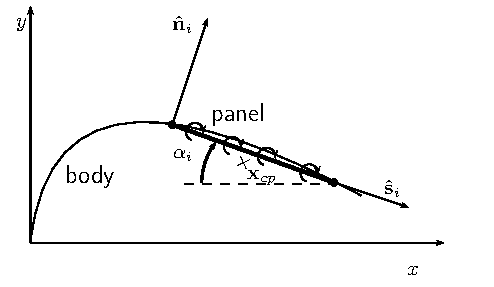
\includegraphics[width=\textwidth]{figures/lagrangian/panelCoordinateDefinition.pdf}
                \caption{Panel discretization of the body in the global cartesian coordinates system $\left(x,y\right)$ with the local panel coordinates system rotated by $\alpha_i$.}
                \label{fig:panelCoordinateDefinition}
        \end{subfigure}%
        ~ %add desired spacing between images, e. g. ~, \quad, \qquad etc.
          %(or a blank line to force the subfigure onto a new line)
        \begin{subfigure}[b]{0.5\textwidth}
                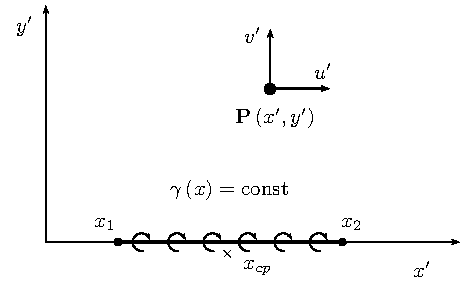
\includegraphics[width=\textwidth]{figures/lagrangian/vortexPanelDefinition.pdf}
                \caption{Constant-Strength Vortex panel in the local panel coordinate system $\left(x',y'\right)$ inducing the velocity $\mathbf{u}'=(u',v')$ on the point $P$.}
                \label{fig:vortexPanelDefinition}
        \end{subfigure}
        \caption{The two coordinate system of the panel method problem. The figure depicts \textbf{(a)} the global panel coordinate system, and \textbf{(b)} the local panel coordinate system, as defined by Katz and Plotkin \cite{Katz2001a}.}
        \label{fig:panelDefinitions}
	\end{figure}	
	
Figure \ref{fig:panelCoordinateDefinition} shows the discretization of the body into panels in the global coordinates system, defined by $(x,y)$, where each panel is rotated by an angle $\alpha_i$ w.r.t to the global coordinate system. Rotating the axis $(x,y)$ by $\alpha_i$, we arrive at the local panel coordinate system $(x',y')$, as shown in figure \ref{fig:vortexPanelDefinition}. Katz and Plotkin \cite{Katz2001a} showed that, the induced velocity of the vortex panels are calculated in the local panel coordinate system, where the induced velocity of the vortex panel $j$ on the collocation point $i$ (in the panel coordinate system) is given as,
	\begin{subequations}
	\begin{align}
	u'_{ij} &= \frac{\gamma_j}{2\pi}\left[\tan^{-1}\frac{y'_i-y'_{j,2}}{x'_i-x'_{j,2}} - \tan^{-1}\frac{y'_i-y'_{j,1}}{x'_i -x'_{j,1}}\right],\\
	v'_{ij} &= -\frac{\gamma_j}{4\pi}\ln\frac{\left(x'_i-x'_{j,1}\right)^2 + \left(y'_i-y'_{j,1}\right)^2}{\left(x'_i-x'_{j,2}\right)^2+\left(y'_i-y'_{j,2}\right)^2}
	\end{align}
	\end{subequations}

where $(x'_1,y'_1)_j$ and $(x'_2,y'_2)_j$ are the coordinates of the panel start and end points in its local panel coordinate system, as shown in figure \ref{fig:vortexPanelDefinition}. The transformation of this vector $(u'_{ij}, v'_{ij})$ to the global coordinates is given as,
	\begin{equation}
	\begin{bmatrix}
	u_{ij}\\
	v_{ij}\\
	\end{bmatrix} = \begin{bmatrix}
	\cos\alpha_j & \sin\alpha_j \\
	-\sin\alpha_j & \cos\alpha_j
	\end{bmatrix} \cdot \begin{bmatrix}
	u'_{ij}\\
	v'_{ij},
	\end{bmatrix}
	\end{equation}

corresponding to a rotation of $\alpha$, as shown in figure \ref{fig:panelCoordinateDefinition}.

If we are dealing with multiple panel bodies (i.e. multiple geometries), as seen in figure \ref{fig:twoPanelBodies}, the panel problem can be solved by constructing a global influence matrix, 
	\begin{equation}
	\underbrace{\begin{pmatrix}
		c_{a_1a_1} & \cdots & c_{a_1a_N} & c_{a_1b_1} &\cdots & c_{a_1b_M}\\
		\vdots & \ddots & \vdots & \vdots &\ddots & \vdots\\
		c_{a_Na_1} & \cdots & c_{a_Na_N} & c_{a_Nb_1} &\cdots & c_{a_Nb_M}\\
		c_{b_1a_1} & \cdots & c_{b_1a_N} & c_{b_1b_1} &\cdots & c_{b_1b_M}\\
		\vdots & \ddots & \vdots & \vdots &\ddots & \vdots\\
		c_{b_Ma_1} & \cdots & c_{b_Ma_N} & c_{b_Mb_1} &\cdots & c_{b_Mb_M}\\
		\Delta s_{a_1} & \cdots & \Delta s_{a_N} & 0 & \cdots & 0\\
		0 & \cdots & 0 & \Delta s_{b_1} & \cdots & \Delta s_{b_M}\\
	\end{pmatrix}
	\begin{pmatrix}
		\gamma_{a_1}\\
		\vdots\\
		\gamma_{a_N}\\
		\gamma_{b_1}\\
		\vdots\\
		\gamma_{b_M}\\
	\end{pmatrix}}_{\begin{pmatrix}
						C_{aa} & C_{ab} \\
						C_{ba} & C_{bb} \\
						\Delta s_a & 0\\
						0 & \Delta s_b \\
					\end{pmatrix} \begin{pmatrix}
								\gamma_{a}\\
								\gamma_{b}\\
							\end{pmatrix}} 
	= 
	\underbrace{\begin{pmatrix}
		\mathrm{RHS}_{a_1}\\
		\vdots\\
		\mathrm{RHS}_{a_N}\\
		\mathrm{RHS}_{b_1}\\
		\vdots\\
		\mathrm{RHS}_{b_M}\\
		\Gamma_{\gamma,a}\\	
	\Gamma_{\gamma,b}
	\end{pmatrix}}_{ 
			\begin{pmatrix}
				\mathrm{RHS}_{a}\\
				\mathrm{RHS}_{b}\\
				\Gamma_{\gamma,a}\\	
				\Gamma_{\gamma,b}
			\end{pmatrix}}
	\end{equation}

where the matrices ($C_{aa}$, $C_{bb}$), are the self-induction matrices of each of the single vortex panel problem. The non-diagonal terms ($C_{ab}$, $C_{ba}$) are the inter-induction matrices containing the panel influence of 
body $b$ on body $a$ and body $a$ on body $b$, respectively. The final two rows of the LHS matrix contain the circulation constraint for each body, defined by equation \ref{eq:la_circualtionConstr}.

	\begin{figure}[t]
	\centering
	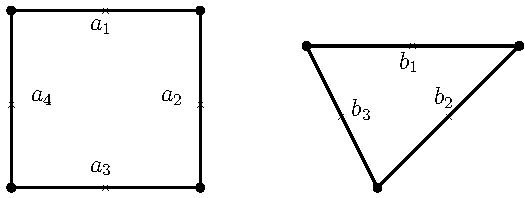
\includegraphics[width=0.6\textwidth]{figures/lagrangian/twoPanelBodies.pdf}
	\caption{Multi-body panel problem: two bodies with different numbers of panels. The figure depicts a square body with 4 panels ($a_1, a_2, a_3, a_4$), and a triangular body with 3 panels ($b_1, b_2, b_3$). }
	\label{fig:twoPanelBodies}
	\end{figure}


%\newpage
%\section{Simulation acceleration techniques}
%\label{sec:sat}
%%
%\subsection{Fast multi-pole Method}
%%
%\subsection{Parallel computation in GPU}


\section{Evolution of the Lagrangian method}

The algorithm of the full Lagrangian method is summarized in this section. The full or complete	Lagrangian method is the coupled vortex blobs and the vortex panels. Note that for our hybrid scheme, the panel does not act as the source of the vorticity in the Lagrangian method (which is done by the Eulerian method), but instead simply enforces the \emph{no-slip} boundary condition for the vortex blobs.
	
	\begin{figure}[!h]
		\centering
		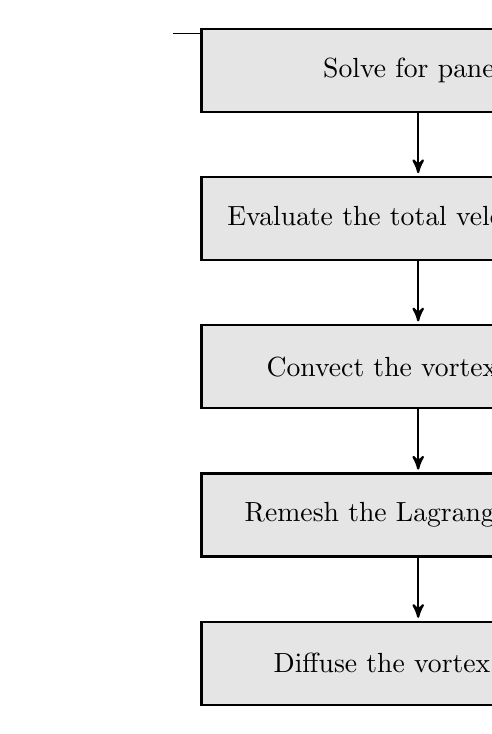
\begin{tikzpicture}
			[node distance=.8cm, start chain=going below,]
			\node[punktchain, join] (solvePanel) {Solve for panels};
		    \node[punktchain, join] (solveVelocity) {Evaluate the total velocity field};
		    \node[punktchain, join] (convect)     {Convect the vortex blobs};
		    \node[punktchain, join] (remesh) 	  {Remesh the Lagrangian field};
		    \node[punktchain, join] (diffuse)     {Diffuse the vortex blobs};		    
		\end{tikzpicture}
		\caption{Flowchart of the Lagrangian method. The flowchart shows coupling between vortex panels and vortex blobs to evolve from $t_n$ to $t_{n+1}$ (without taking into account of the vorticity generation at the boundary).}
		\label{fig:flowchart_lagrangian}
	\end{figure}	
	
The flowchart of one time step of the Lagrangian method is given by figure \ref{fig:flowchart_lagrangian}.The algorithm to the Lagrangian method can be summarized as follows:
	\begin{enumerate}
	\item \textbf{Solve for panels:} Determine the strengths of the vortex panels $\gamma$, such that the no-slip boundary condition at the collocation points of the vortex panels is enforced. When determining the strengths, we also have to ensure that the total circulation of the vortex panels satisfies the conservation of circulation, equation \ref{eq:circulationConstraintonPanels}, which we investigate during the hybrid coupling, section \ref{subsubsec:cc}.
	\item \textbf{Evaluate the total velocity field:} Evaluate the total velocity field $\mathbf{u}$, which is the sum of velocity field induced by the vortex blobs $\mathbf{u}_{\omega}$, the velocity field induced by the vortex panels $\mathbf{u}_{\gamma}$, and the free-stream velocity field $\mathbf{u}_{\infty}$. 
	\item \textbf{Convect the vortex blobs:} Use the velocity field to convect the vortex blobs from $t_n$ to $t_{n+1}$ to the new position.
	\item \textbf{Remesh the Lagrangian field:} Remesh the vortex blobs onto a structured square lattice using the $\mathrm{M}'_4$ interpolation kernel.
	\item \textbf{Diffuse the vortex blobs:} Diffuse the vortex blobs using the $\Delta t_d$ diffusion time step, by modifying the strengths of the vortex blobs according to Wee's WRS or Tutty's TRS method.
	\end{enumerate}

The generation of the vorticity is dealt with in the Eulerian domain, which is explained in chapter \ref{ch:eulerian}. The vorticity is then transfered into the Lagrangian domain using the Hybrid coupling scheme, which was summarized in the introduction, chapter \ref{ch:introduction}, and fully elaborated in chapter \ref{ch:hybrid}.

%
\section{Validation of Lagrangian method}
\label{sec:volm}
In this chapter, we have investigated the Lagrangian component of the Hybrid method. The Lagrangian method is used to just evolve the vorticity field, where as the Eulerian method is used to properly formulate the vorticity generation at the boundary. The resolved boundary solution of the Eulerian method is then transfered onto our Lagrangian method. Therefore, the Lagrangian method that is implemented here does not require the generation of the vorticity from the boundary. 

Thus, during the validation of the Lagrangian method, we focus on two test cases: Potential flow around a cylinder and Lamb-Oseen vortex evolution. The potential flow around a cylinder test case is used to verify and validate the vortex panel solver that is used enforcing the no-through flow for the vortex blobs. The Lamb-Oseen vortex evolution test cases is used to verify and validate the convection method and the diffusion methods implemented for the evolution of the vortex blobs.

Note that to investigate the coupling of the vortex blobs and the vortex panels, we require the proper definition of the vorticity flux from the boundary, requiring the Eulerian method as well. Therefore, the handling of the vorticity flux is investigated in fully coupled method, in chapter \ref{ch:vavohm}.


\subsection{Error analysis of vortex panels}

	\ctable[
	    caption = {Panel study parameters},
	    label   = {tab:panelParams},
	    pos = b,
	]{lll}{}{\FL
	Parameters 				& Value 			& Description \ML
	$R$  					& 1 \si{m} 			& Radius of cylinder\\
	$u_{\infty}$	& 1 \si{m.s^{-1}}	& Free-stream velocity\\
	$N_{\mathrm{panels}}$	& 100				& Number of panels\LL}	

The vortex panels was verified and validated on the test case of the potential flow around a cylinder. To test the 
convergence of the solution of the vortex panels, a comparison was made with the analytical solution for the parameters in table \ref{tab:panelParams}.

An example of the numerical solution is shown in figure \ref{fig:panelCylinder_velocityField}. The figure shows the magnitude of the velocity $\lVert\mathbf{u}\rVert|$, and it shows the velocity field of the potential flow solution, with an infinitely thin boundary layer, stagnating to zero velocity inside the body.

	\begin{figure}[p]
	\centering
	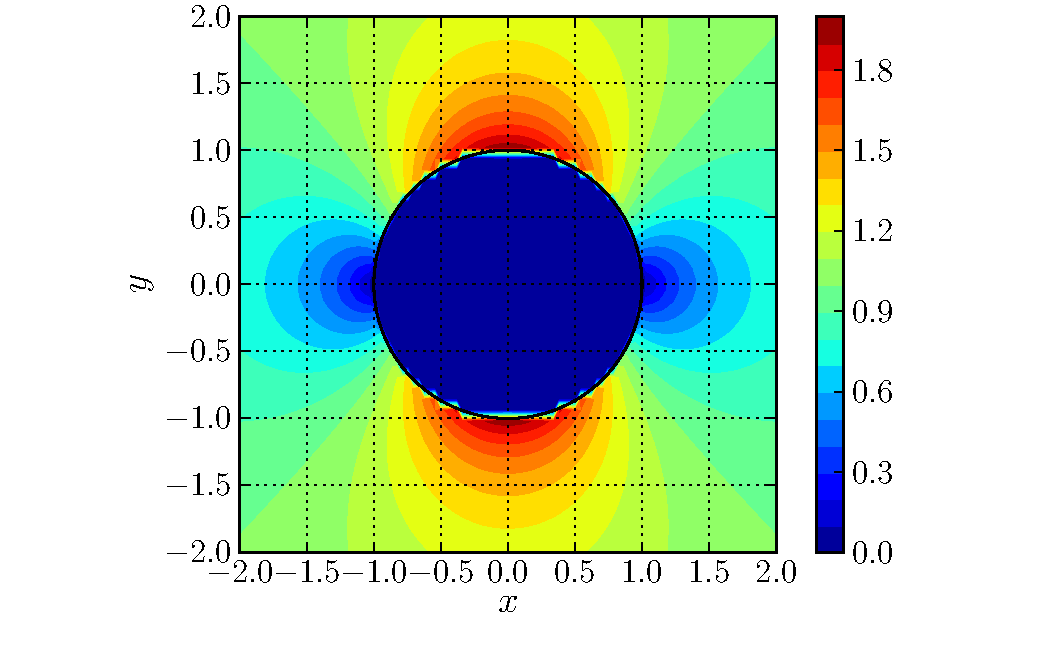
\includegraphics[width=0.7\textwidth]{figures/lagrangian/panelCylinder_velocityField.pdf}
	\caption{Panel method solution: the potential velocity field around a unit cylinder with $R = 1$, $\mathbf{u}_{\infty} = (1, 0)$, and $N_{\mathrm{panels}}=100$. The figure depicts the magnitude of velocity field $\left\Vert\mathbf{u}\right\Vert$, with a zero velocity inside the body.}
	\label{fig:panelCylinder_velocityField}
	\end{figure}

	\begin{figure}[p]
     \centering
     \begin{subfigure}[b]{0.5\textwidth}
             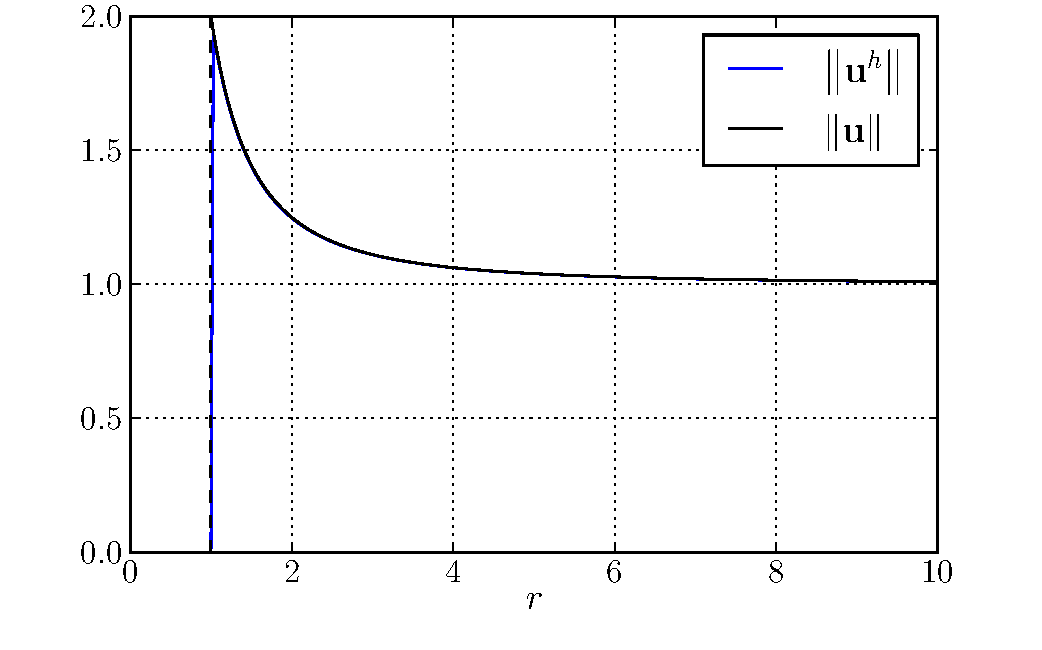
\includegraphics[width=\textwidth]{figures/lagrangian/panelCylinder_versusAnalytical.pdf}
             \caption{Comparison of the velocity field.}
             \label{fig:panelCylinder_versusAnalytical}
     \end{subfigure}%
     ~ %add desired spacing between images, e. g. ~, \quad, \qquad etc.
       %(or a blank line to force the subfigure onto a new line)
     \begin{subfigure}[b]{0.5\textwidth}
             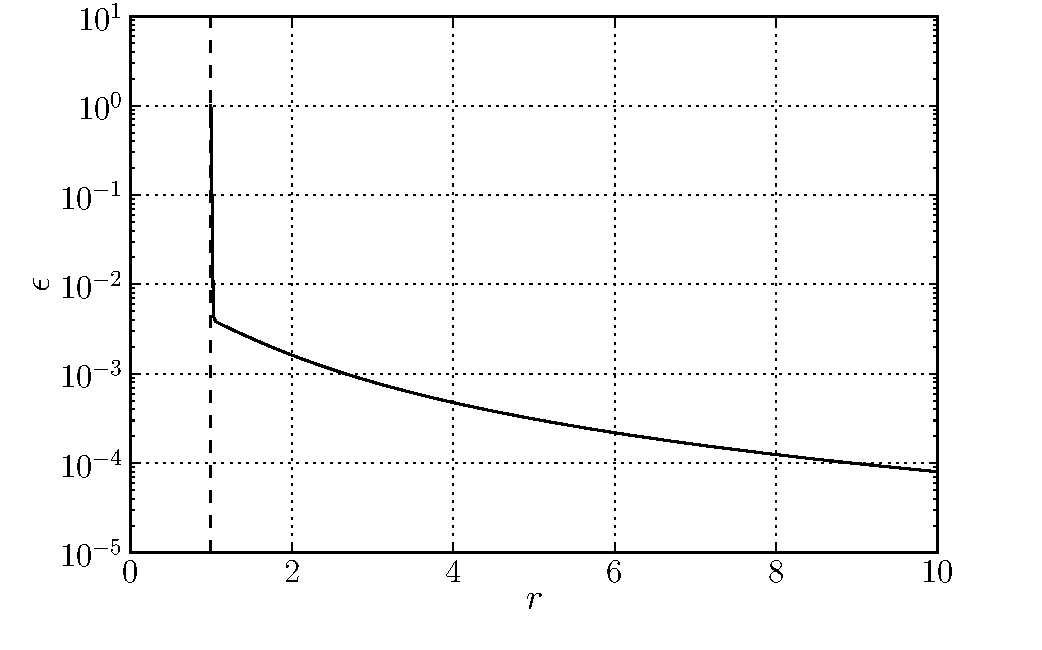
\includegraphics[width=\textwidth]{figures/lagrangian/panelCylinder_error.pdf}
             \caption{Error in the velocity field}
             \label{fig:panelCylinder_error}
     \end{subfigure}
     \caption{Comparison of the velocity field along the $y$-axis, $y=0$ to $y=10$. Figure \textbf{(a)} shows both the solutions, the numerical $\left\Vert\mathbf{u}^h\right\Vert$ [{\color{plotBlue}{---}}, solid {\color{plotBlue}{\textbf{blue}}}] and the analytical solution [---, solid \textbf{black}]. Figure \textbf{(b)} shows the relative error $\epsilon$ in velocity between the solution, given by equation \ref{eq:panelRelativeError}.}
     \label{fig:panelCylinderComparision}
	\end{figure}

	\begin{figure}[p]
	\centering
	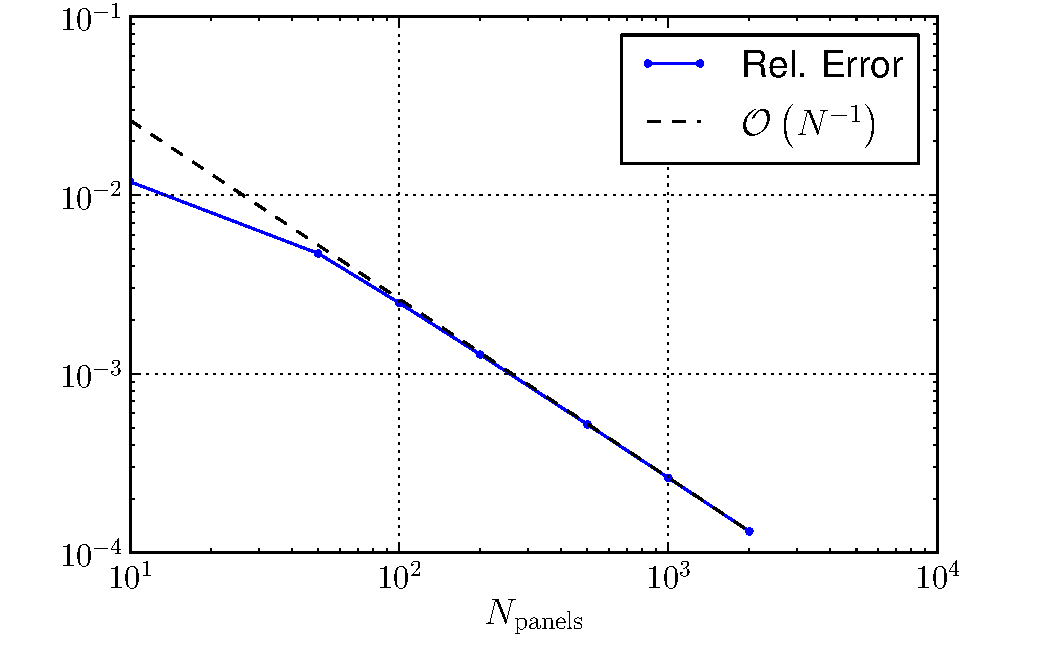
\includegraphics[width=0.5\textwidth]{figures/lagrangian/panelCylinder_convergence_compressed.pdf}
	\caption{Convergence plot of the Constant-Strength Straight Vortex panels. The figures depicts the converges of the relative error $\epsilon$ at an $\mathcal{O}\left(N^{-1}\right)$.}
	\label{fig:panelCylinder_convergence}
	\end{figure}


The jagged velocity field around the surface of the cylinder is simply due to the sampling resolution of the field. For a higher sampling resolution this will vanish. In order to determine the accuracy of the solution, the velocity field of the panel solution was compared with the analytical solution. The analytical velocity field around a cylinder is given in cylindrical coordinate centered in the cylinder as,
	\begin{subequations}
	\begin{align}
	u_r &= u_{\infty}\left(1 - \frac{R^2}{r^2}\right)\cos\theta,\\
	u_{\theta} &= -u_{\infty}\left(1+\frac{R^2}{r^2}\right)\cos\theta,
	\end{align}
	\label{eq:potentialCylinderAnalytical}
	\end{subequations}	
where $u_r$ and $u_{\theta}$ are the radial and the angular velocity respectively for a given free-steam velocity $u_{\infty}$. Equation \ref{eq:potentialCylinderAnalytical} is a function of the distance to the center of the cylinder $r$ and the radius of the cylinder $R$ and is valid for $r\geqslant{R}$

The velocity field of the vortex panel was compared with the analytical solution along the y-axis from $y=0$ to $y=10$. Figure \ref{fig:panelCylinder_versusAnalytical} plots the magnitude of analytical velocity $\left\Vert\mathbf{u}\right\Vert$ and the vortex panel velocity field $\left\Vert\mathbf{u}^h\right\Vert$. Comparing the solutions of the plot we see that the solution of the vortex panels and the analytical potential flow solution matches everywhere except at the surface. This happens because the potential flow solution has a slip velocity (i.e non-zero velocity) at the surface of the body, whereas the vortex panels solves for a no-slip boundary condition at the collocation points of the surface. This explains the sudden drop of the velocity from $\lVert\mathbf{u}\rVert = 2$ to $\lVert\mathbf{u}\rVert = 0$ at the surface.	

Figure \ref{fig:panelCylinder_error} shows the relative error $\epsilon$ between the numerical and the analytical solutions,
	\begin{equation}
	\epsilon = \frac{\left\Vert\mathbf{u}-\mathbf{u}^h\right\Vert}{\left\Vert\mathbf{u}\right\Vert}
	\label{eq:panelRelativeError}
	\end{equation}
	
where $\mathbf{u}$ is the analytical solution and the $\mathbf{u}^h$ is the numerical solution. Ignoring the solution right at the surface ($r=R$), we see that the error between the numerical and the analytical solution reduces from $\epsilon=\num{5e-3}$ to $\epsilon=\num{8e-5}$ as we go from $r=1$ to $r=10$. This behavior of the error tells us that the solution of the constant-strength vortex panels gets more accurate as we go further away from the panels; right next to the panels, we have the largest error.

The convergence analysis of the vortex panels was done by determining the error of the vortex panel velocity field w.r.t to the analytical solution for the number of panels $N = 10$ to $N = 1000$, figure \ref{fig:panelCylinder_convergence}. The error of the velocity field was computed at $(x =0, y=1.5)$, and we see that the error converges at with $\mathcal{O}\left(N\right)$. This validates that the vortex panel that we have used is a $1^{\mathrm{st}}$ order vortex panel.

\subsection{Error analysis of vortex blobs}
\label{subsec:lagrangianLambOseen}
In order to verify and validate the vortex blobs, we simulate the evolution of a Lamb-Oseen vortex. The results of the simulation were used to compare against the analytical ones, which we used to determine the accuracy of our vortex blobs.

The Lamb-Oseen vortex is a solution of the Navier-Stokes equation, corresponding to the viscous evolution of a laminar vortex core on an unbounded domain, first derived by Lamb and Oseen \cite{Tryggeson2007}. The vorticity distribution $\omega$ of the core at a given time is defined as,

	\begin{equation}
	\omega\left(\mathbf{x},\tau\right) = \frac{\Gamma_c}{4\pi\nu(t+\tau)} \exp\left(-\frac{r^2}{4\pi\nu(t+\tau)}\right),
	\label{eq:lo_voeq}
	\end{equation}

and is a function of core strength $\Gamma_c$, the simulation time $t \in [0,\infty[$ and distance from the core center $r$. The constant $\tau$ in the equation \ref{eq:lo_voeq} defines to initial width of the Lamb-Oseen vortex, where if $\tau=0$, we have Dirac delta distribution.

The velocity field, corresponding to equation \ref{eq:lo_voeq}, in cylindrical coordinate is defined as,

	\begin{subequations}
	\begin{align}
	u_{\theta} &= \frac{\Gamma_c}{2\pi r} \left[1-\exp\left(-\frac{r^2}{4\pi\nu(t+\tau)}\right)\right]\\
	u_r &= 0
	\end{align}
	\label{eq:lo_veeq}
	\end{subequations}

where $u_{\theta}$ is the circumferential velocity, and $u_r$, the radial velocity is zero. Figure \ref{fig:lambOseen_distributions} shows the vorticity distribution $\omega$ for various initial time constant $\tau$. We see that for small $\tau$, the distribution approaches a Dirac delta distribution. Therefore, for this investigation we decided on $\tau=4$ ensuring a non-peaky distribution, which was also investigated by Barba \cite{Barba2004c}.  Therefore the literature of Barba \cite{Barba2004c} will serve as the validation data for our Lamb-Oseen investigation.


%	\begin{figure}[!t]
%        \centering
%        \begin{subfigure}[b]{0.5\textwidth}
%                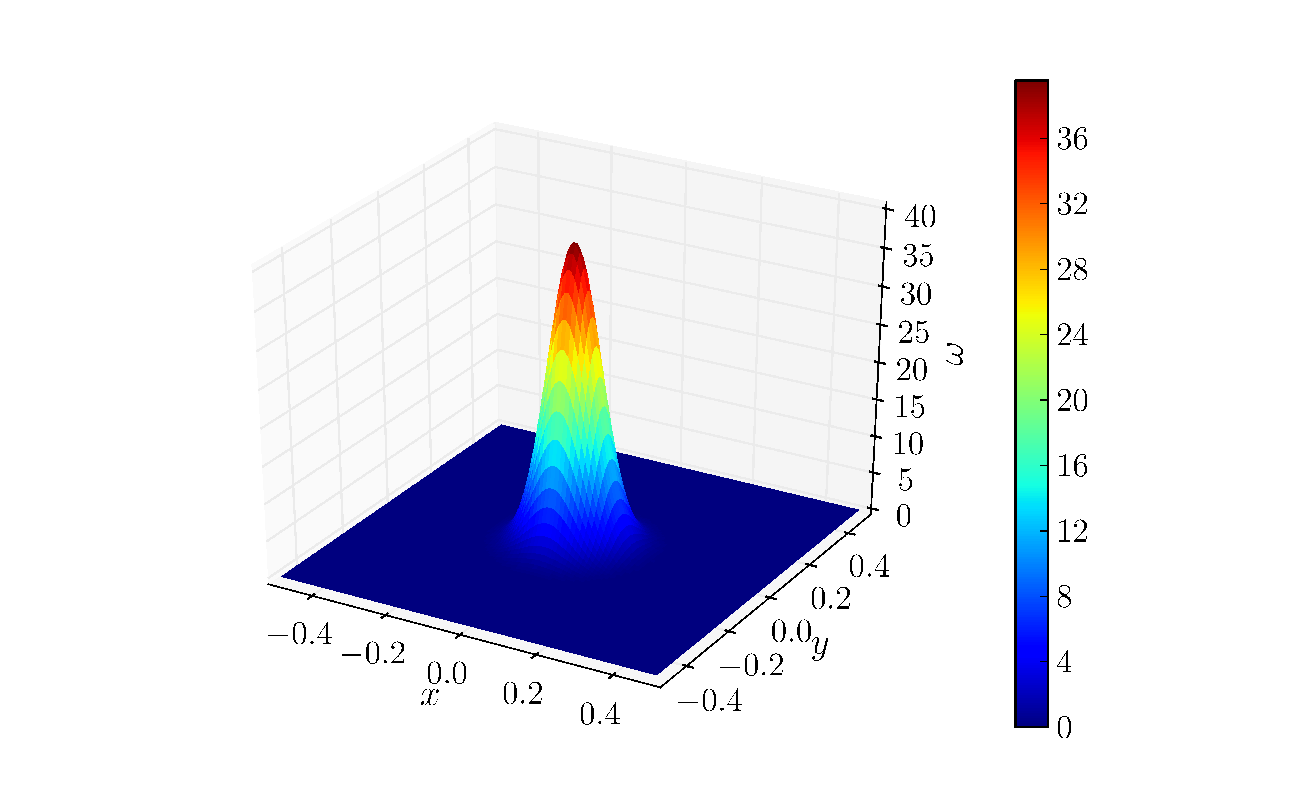
\includegraphics[width=\textwidth]{figures/lagrangian/lambOseen_vorticityDistribution_compressed.pdf}
%                \caption{Vorticity field}
%                \label{fig:lambOseen_vorticityDistribution}
%        \end{subfigure}%
%        ~ %add desired spacing between images, e. g. ~, \quad, \qquad etc.
%          %(or a blank line to force the subfigure onto a new line)
%        \begin{subfigure}[b]{0.5\textwidth}
%                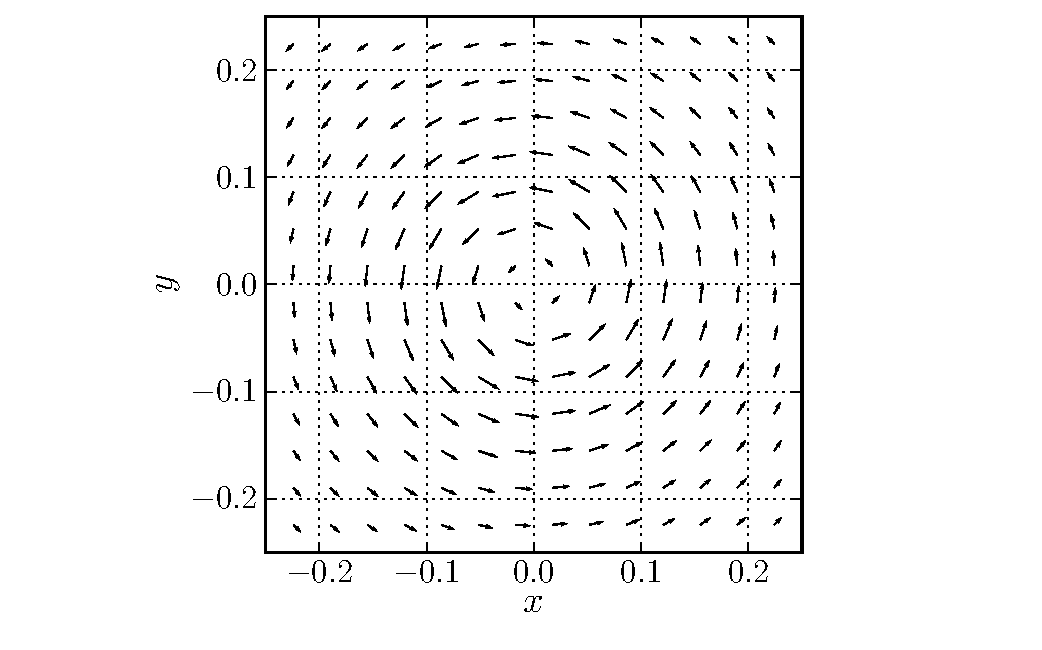
\includegraphics[width=\textwidth]{figures/lagrangian/lambOseen_velocityDistribution_compressed.pdf}
%                \caption{Velocity Field}
%                \label{fig:lambOseen_velocityDistribution}
%        \end{subfigure}
%        
%        
%        \caption{Lamb-Oseen Vortex problem with $\Gamma_c = 1$, $\tau=\num{2e-3}$, and $\nu=\num{5e-4}$. The figure depicts \textbf{(a)} the vorticity distribution, and \textbf{(b)} the velocity distribution.}
%        \label{fig:lambOseen_distributions}
%	\end{figure}

	\begin{figure}[!t]
        \centering
        \begin{subfigure}[b]{0.3\textwidth}
                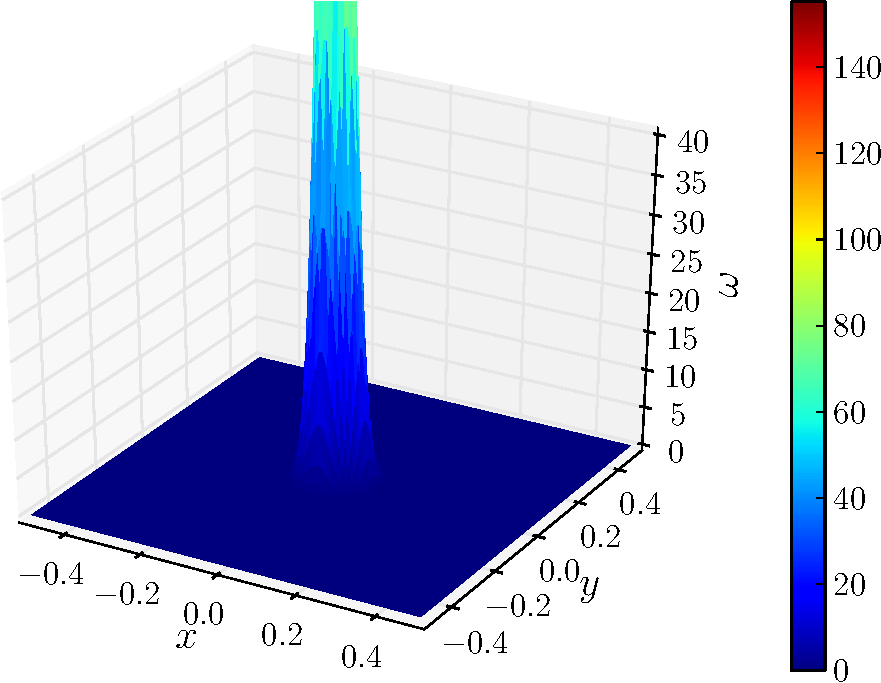
\includegraphics[width=\textwidth]{figures/lagrangian/lambOseen_definition_tau=1-crop.pdf}
                \caption{$\tau = 1$}
                \label{fig:lambOseen_tau1}
        \end{subfigure}%
        ~ %add desired spacing between images, e. g. ~, \quad, \qquad etc.
          %(or a blank line to force the subfigure onto a new line)
        \begin{subfigure}[b]{0.3\textwidth}
                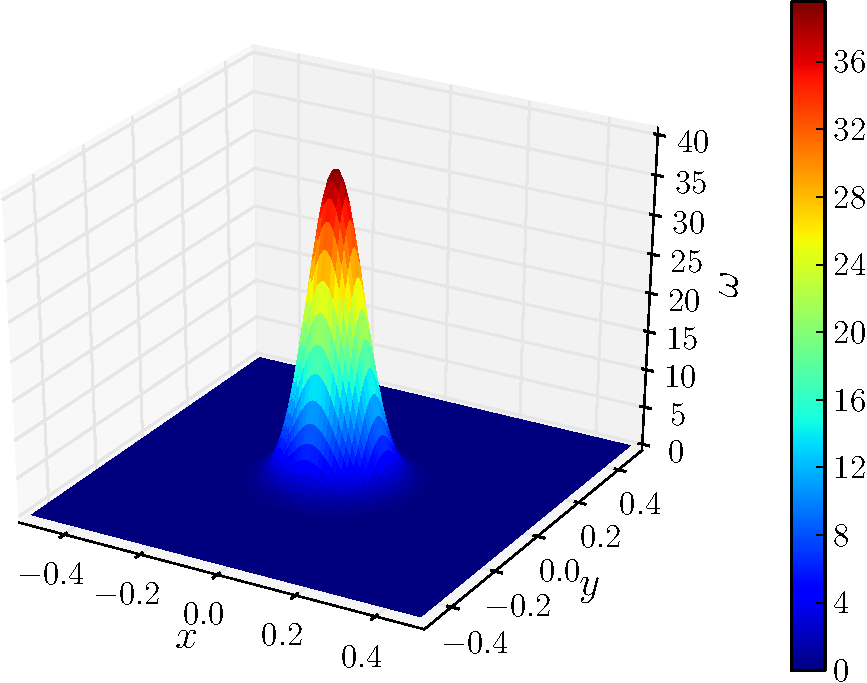
\includegraphics[width=\textwidth]{figures/lagrangian/lambOseen_definition_tau=4-crop.pdf}
                \caption{$\tau = 4$}
                \label{fig:lambOseen_tau4}
        \end{subfigure}
		~
        \begin{subfigure}[b]{0.3\textwidth}
                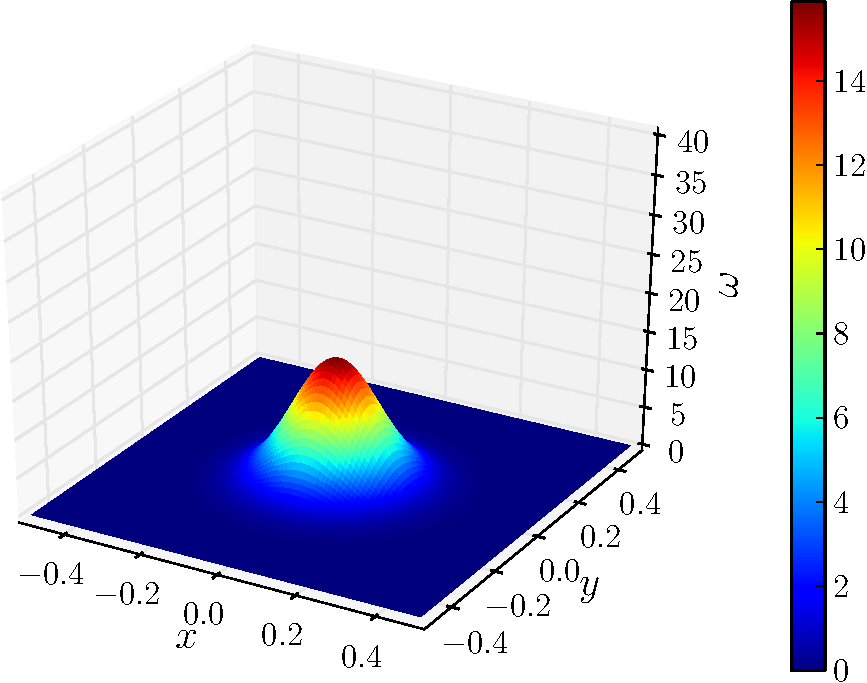
\includegraphics[width=\textwidth]{figures/lagrangian/lambOseen_definition_tau=10-crop.pdf}
                \caption{$\tau = 10$}
                \label{fig:lambOseen_tau10}
        \end{subfigure}        
        
        \caption{The vorticity $\omega$ distribution of the Lamb-Oseen vortex problem with $\Gamma_c = 1$ and $\nu=\num{5e-4}$ in the domain $[-0.5,0.5]\times[-0.5,0.5]$. The figure depicts distribution for various initial time constant $\tau$, determining the peakiness of the distribution.}
        \label{fig:lambOseen_distributions}
	\end{figure}
	
	
	\ctable[
		caption = {Summary of the parameters for the Lamb-Oseen vortex evolution. This table shows also the parameters of Tutty's diffusion method},
		label   = {tab:lambOseenParams},
		pos = !b,]{lcll}{}{\FL
		
		Parameters 					& Value 	& Unit					& Description \ML
		$\Gamma_c$\T               	& 1 &\si{m^2.s^{-1}} 				& Core strength\\
		$\Omega$               		& $\left[-0.5,0.5\right]\times\left[-0.5,0.5\right]$ &\si{m}	& Initial particle domain \\
		$\mathbf{u}_{\infty}$ 		& $0$ &\si{m.s^{-1}} & Free-stream velocity\\
		$\nu$						& $\num{5e-4}$ &\si{kg.s^{-1}.m^{-1}}& Kinematic viscosity\\
		$ \tau$ 		    		& 4		& \si{s}					& Lamb-Oseen time constant\\
		$ t$ 		    	& \numrange{0}{1} &\si{s}			& Simulation time\\		
		$ \Delta t_c = \Delta t_d$ 	& $0.01$ &\si{s}						& Diffusion and convection time step size\\
		$ N_{\mathrm{t-steps}}$ 	& 100 & -						& Number of time integration steps\\		
		$ \sigma$ 					& $0.01$ &\si{m}						& Vortex blob core size\\	        
		$ \lambda$			& $1$	& -							& Overlap ratio\\	        	        
		$ k$						& $2$	& -							& Gaussian kernel width spreading\\
		$ f_{redis}$		& $1$ 	& -							& Redistribution frequency\\	        	        
		$ f_{pc}$		& $1$  & -							& Population control frequency\\	        	        
		$ (\Gamma_{loc},\Gamma_{glob})$ & $(\num{1e-14},\num{1e-14})$ &\si{m^2.s^{-1}} & Population control thresholds\LL}	

The Lagrangian method was applied to the Lamb-Oseen vortex test case with parameters tabulated in table \ref{tab:lambOseenParams}. The vorticity field was discretized over the domain $[x,y]$ - domain $\left[-0.5,0.5\right]\times\left[-0.5,0.5\right]$. This was adequate as the circulation outside this domain was less that the threshold $\Gamma_{loc}\le\num{e-14}$. The spatial discretization was performed according to the standard initialization method of vortex blobs, described in section \ref{subsec:vortexBlobInitialization}.

However as explained in section \ref{subsec:vortexBlobInitialization}, we have to take in account of the Gaussian blurring of the original vorticity field due to the initialization process. This poses a problem when evaluating the error between the numerical and the analytical solution. This problem has also been encountered by Barba \cite{Barba2004c}, when investigating the Lamb-Oseen vortex. The solution to the problem was to apply a ``time-shift correction", to compensate for the Gaussian blurring, solving the problem of this very particular discretization of the Navier-Stokes equation. Therefore, this is a special method and this approach can only be used for the Lamb-Oseen vortex problem.

The ``time-shift correction" is derived by determining the diffusion effect caused by the discretization of the diffusion equation using the Gaussian vortex blobs (with $k=2$). Barba \cite{Barba2004c}, determined that the discretization of the diffusion equation (i.e. the Lamb-Oseen vortex) reconstructs the vorticity field that has been diffused by a time $\sigma^2/2\nu$. So when initializing the particles with a certain strength, we will have to reverse the time by $\sigma^2/2\nu$. Thus, the corrected initial particles strengths $\alpha_i^o$ of vortex blobs from the Lamb-Oseen vorticity field is given as,

	\begin{equation}
	\alpha_i^o = \omega_i^o\cdot h^2 = \left\{ \frac{\Gamma_c}{4\pi\nu\left(t+\tau-\sigma^2/2\nu\right)} \exp\left[-\frac{r_i^2}{4\nu\left(t+\tau-\sigma^2/2\nu\right)}\right] \right\} \cdot h^2.
	\label{eq:lo_pie}
	\end{equation}
	
This method was used to investigate the error evolution of the vortex blob method. The vortex blobs where convected according to the procedures in section \ref{sec:covb}. The diffusion of the vortex blobs was performed using the schemes described in section \ref{sec:diffusionVM}. We investigated the accuracy of the Tutty's scheme (TRS) and Wee-Ghoniem scheme (WRS) in section \ref{subsubsec:comp_wrs_trs}. For the general investigation however, we employed the Tutty's diffusion method. The advantage of this approach is that the we can perform diffusion after every convection step. This makes the method less prone to time integration error and eliminates any discontinuous behavior in the evolution. We will see that when coupling the Lagrangian method and Eulerian method, discontinuity in the problem introduces additional errors.

%	\begin{figure}[p]
%	\centering
%	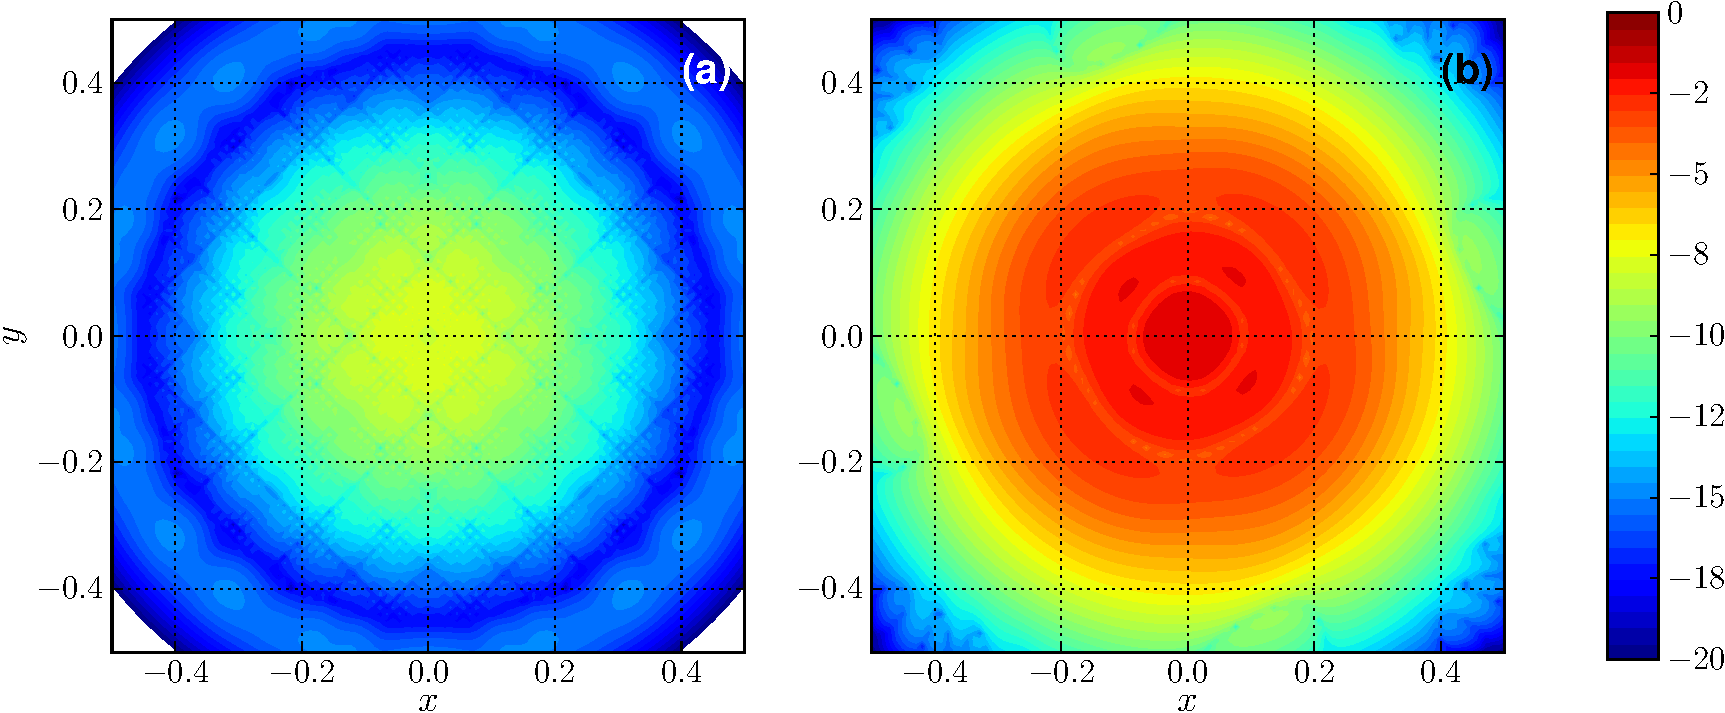
\includegraphics[width=0.99\textwidth]{figures/lagrangian/lambOseen_convection_vorticityErrorContours_compressed-crop.pdf}
%	\caption{Relative error growth of Lamb-Oseen vorticity during the evolution (in logarithmic scale). The figure shows \textbf{(a)}, the initial relative error at $t_0=4$, and \textbf{(b)} the final relative error in vorticity at $t_f=5$.}
%	\label{fig:lambOseen_convection_vorticityErrorContours_compressed}
%	\end{figure}
%	
	


The convection and diffusion was performed according to the time integration parameters tabulated in table \ref{tab:lambOseenParams}. The vortex blobs where convected using a $4^{\mathrm{th}}$-order Runge-Kutta method ($\mathrm{RK4}$) for a high order time integration. After the convection sub-steps, the Lagrangian distortion was treated using the remeshing scheme discussed in section \ref{subsec:remeshing}. Generally, the remeshing is typically done every 10 iterations \cite{Barba2004c}. However, as our diffusion scheme and hybrid method requires structured lattice of vortex blobs for efficient calculations, we will remesh after every step, $f_{\mathrm{redist}}=1$.  


In addition to the evolution of the vortex blobs, we performed a population control to minimized the number of vortex blobs, as described by Barba \cite{Barba2004c}. The \indexAcron{Population Control}{PC} removes vortex blobs that have very small circulation strengths. After the diffusion and remeshing, we will be left with vortex blobs with strengths close to the numerical precision, as they have minimal impact on the accuracy of the vorticity field, we can removed them. When performing population control, we need to ensure that the loss of total circulation is below the acceptable global threshold, $\Gamma_{glob}$. We used $\Gamma_{glob}=\num{e-14}$ as used by Barba \cite{Barba2004c} for the similar investigation. 

	\begin{figure}[!h]
     \centering
     \begin{subfigure}[b]{0.5\textwidth}
             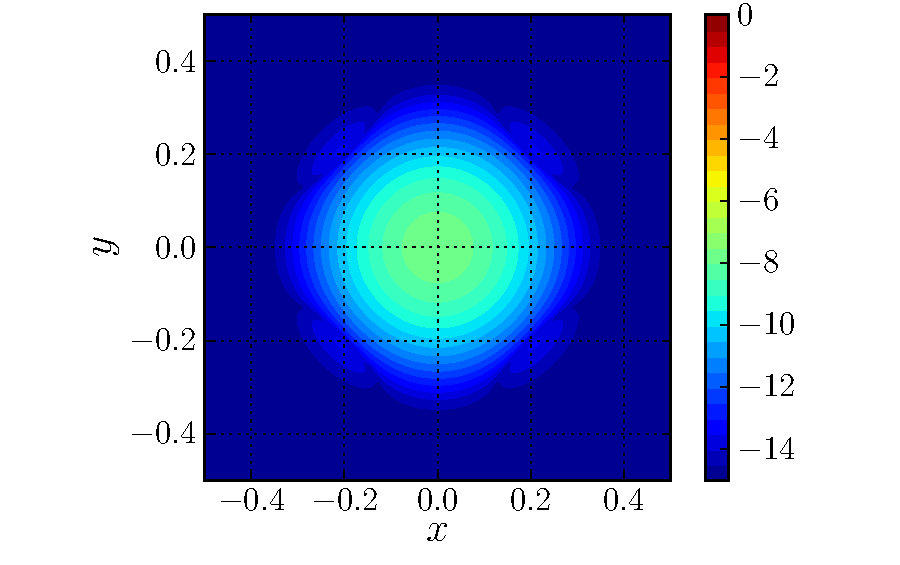
\includegraphics[width=\textwidth]{figures/lagrangian/lambOseen_intialError_wRel.pdf}
             \caption{Vorticity field}
             \label{fig:lambOseen_convection_vorticityErrorContours_initial}
     \end{subfigure}%
     ~ %add desired spacing between images, e. g. ~, \quad, \qquad etc.
       %(or a blank line to force the subfigure onto a new line)
     \begin{subfigure}[b]{0.5\textwidth}
             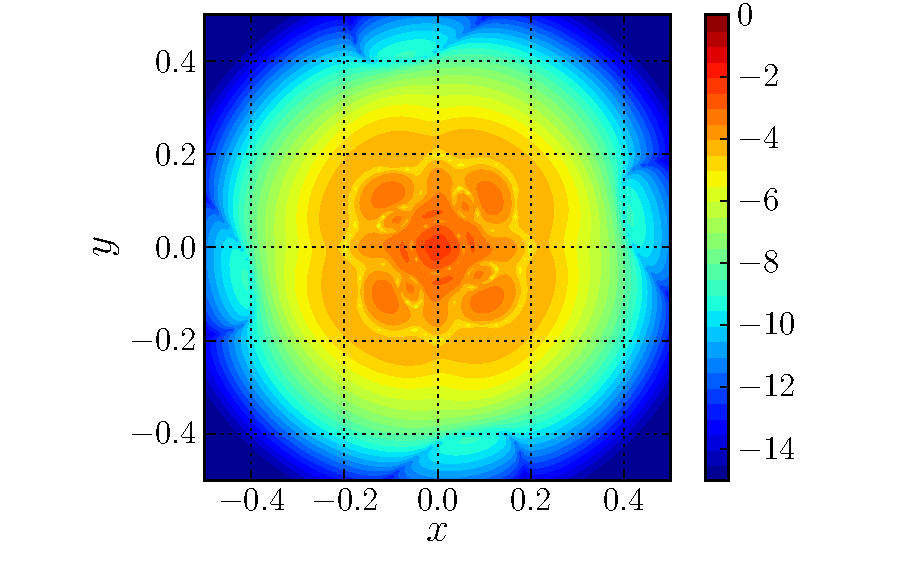
\includegraphics[width=\textwidth]{figures/lagrangian/lambOseen_finalErrorEvolution_wRel.pdf}
             \caption{Velocity Field}
             \label{fig:lambOseen_convection_vorticityErrorContours_final}
     \end{subfigure}
     
     \caption{Relative error growth of Lamb-Oseen vorticity during the evolution (in logarithmic scale) using the parameters tabulated in table \ref{tab:lambOseenParams}. The figure shows \textbf{(a)}, the initial relative error at $t=0$, and \textbf{(b)} the final relative error in vorticity at $t=1$.}
     \label{fig:lambOseen_convection_vorticityErrorContours}
	\end{figure}

To verify whether our Lagrangian scheme is performs according to theory, we evaluated the error evolution of the simulation. Figure \ref{fig:lambOseen_convection_vorticityErrorContours}, shows the initial and the final relative error in vorticity. We see that initially we have a maximum relative error around \num{e-8}, located at the center of the Lamb-Oseen core. After 100 time integration steps from $t=0$ to $t=1$, we see that the maximum relative error in vorticity increases from \num{e-8} to \num{e-2}. The errors of the vorticity are predominantly localized at the center of the core, where we have maximum vorticity, figure \ref{fig:lambOseen_convection_vorticityErrorContours}.

Figure \ref{fig:lambOseen_convection_errorGrowth_compressed}, shows the maximum relative error, equation \ref{eq:maxRelErrorDef}, and the $L^2-\mathrm{norm}$, equation \ref{eq:l2normeq}, error evolution of vorticity and velocity from $t=0$ to $t=1$. Similar investigation was performed by Barba \cite{Barba2004c} and Speck \cite{Speck2011a}. Due to the relation of the vorticity and the velocity, equation \ref{eq:lag_vort}, the error of the vorticity is higher that the error in the velocity. The figure shows both the maximum relative error, and the error in the $L^2-\mathrm{norm}$. The maximum relative error (e.g. for vorticity), is defined as,
	\begin{equation}
	\left\Vert \omega^{\mathrm{exact}} - \omega^{\mathrm{discrete}} \right\Vert_{\infty} = \frac{\max\{\left|\omega^{\mathrm{exact}} - \omega^{\mathrm{discrete}}\right|\}}{\max\{\left|\omega^{\mathrm{exact}}\right|\}},
	\label{eq:maxRelErrorDef}
	\end{equation}
where $\omega^{\mathrm{exact}}$ is the analytical vorticity field, equation	\ref{eq:lo_voeq}, and $\omega^{\mathrm{discrete}}$ is the numerical vorticity field from the vortex blobs. The error in the $L^2-\mathrm{norm}$ of the vorticity is calculated as 

	\begin{equation}
	\left\Vert \omega^{\mathrm{exact}} - \omega^{\mathrm{discrete}} \right\Vert_2 = \left(\sum_{i}^{N}\left| \omega^{\mathrm{exact}} - \omega^{\mathrm{discrete}} \right|^2 \cdot h^2\right)^{\frac{1}{2}},
	\label{eq:l2normeq}
	\end{equation}

and the error in velocity is calculated using the same principle. Investigating the figure, we see that after the first iteration, there is a sudden increase in the error, but as time progresses the error growth reduces. From literature, we see that this trend has also been observed by Barba \cite{Barba2004c} and Speck \cite{Speck2011a}. For comparison, we used similar parameters, and we observe that the sudden jump in error is similar to the literature.

	\begin{figure}[!h]
	\centering
	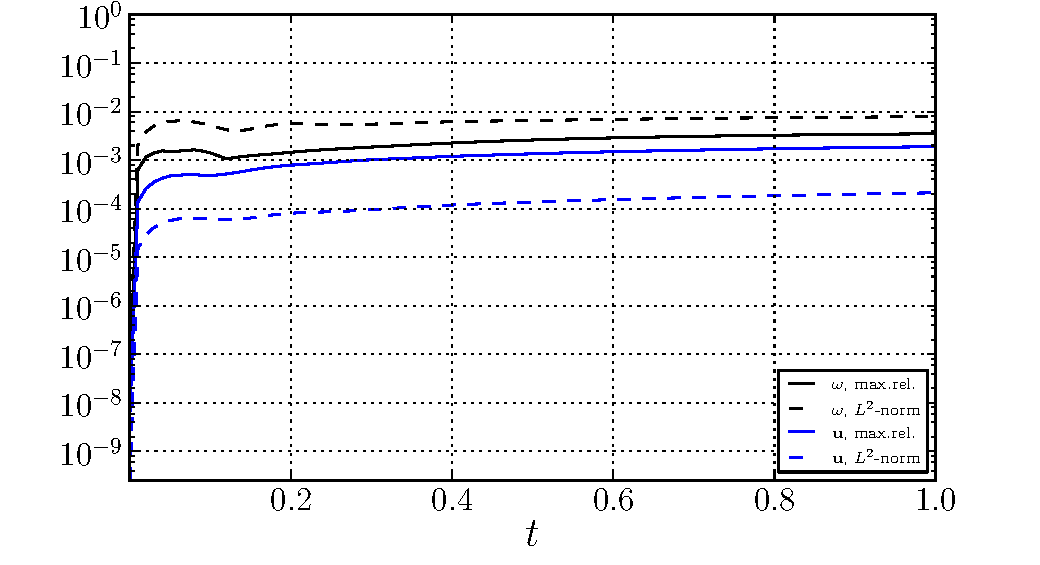
\includegraphics[width=0.6\textwidth]{figures/lagrangian/lambOseen_errorEvolution_TRS_dt0p01.pdf}
	\caption{Relative error growth of Lamb-Oseen vortex during the evolution from $t=0$ to $t=1$ using the parameters in table \ref{tab:lambOseenParams}. This figure depicts the error in vorticity: maximum relative error [ ---, solid \textbf{black}], and the error in $L^2-\mathrm{norm}$ [ - -, dashed \textbf{black}]; and error in velocity: maximum relative error [ {\color{plotBlue}{---}}, solid {\color{plotBlue}{\textbf{blue}}}], and error in $L^2-\mathrm{norm}$ [ {\color{plotBlue}{- -}}, dashed {\color{plotBlue}{\textbf{blue}}}].}
	\label{fig:lambOseen_convection_errorGrowth_compressed}
	\end{figure}
	
\subsubsection{Comparison of diffusion schemes: WRS vs. TRS}
\label{subsubsec:comp_wrs_trs}
To observe how both the diffusion schemes compare, we ran the same test case with both diffusion schemes. From the simulation, we were able to observe that Tutty's diffusion scheme (TRS), produced less error than Wee's approach (WRS). 

Figure \ref{fig:lambOseen_diffusionMethod_comparison} shows the evolution of maximum relative error in vorticity, equation \ref{eq:maxRelErrorDef} for both diffusion schemes. Figure \ref{fig:lambOseen_errorEvolution_WRSvsTRS_dt0p01} shows the evolution of error for convective time step size $\Delta t_c = 0.01$. The diffusion scheme TRS enables us to perform diffusion in conjunction with the convection, $\Delta t_d = \Delta t_c = 0.01$. This was possible due to the favorable constraint on the diffusion time step, equation \ref{eq:TRS_difftimeconstr}.

The Wee's diffusion scheme WRS, however is constraint by equation \ref{eq:c2stability} and equation \ref{eq:la_dtcts}. Therefore the diffusion time step $\Delta t_d$ for the given convective time step $\Delta t_c = 0.01$ is $\Delta t_d = k_d \cdot \Delta t_c = 0.07$, where the diffusion frequency $k_d=7$. We observe from the figure that performing diffusion at every other instant creates an oscillatory behavior. This behavior is not ideal when coupling with the Eulerian method as the oscillatory diffusion of the VPM will add additional error in coupling.

\begin{figure}[!h]
  \centering
  \begin{subfigure}[b]{0.5\textwidth}
          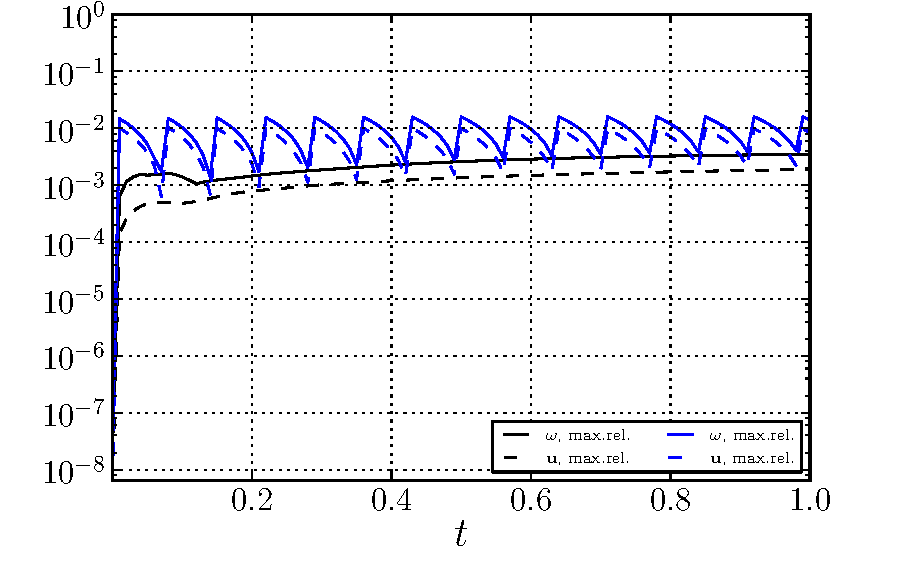
\includegraphics[width=\textwidth]{figures/lagrangian/lambOseen_errorEvolution_WRSvsTRS_dt0p01.pdf}
          \caption{$\Delta t_c = 0.01$}
          \label{fig:lambOseen_errorEvolution_WRSvsTRS_dt0p01}
  \end{subfigure}%
  ~ %add desired spacing between images, e. g. ~, \quad, \qquad etc.
    %(or a blank line to force the subfigure onto a new line)
  \begin{subfigure}[b]{0.5\textwidth}
          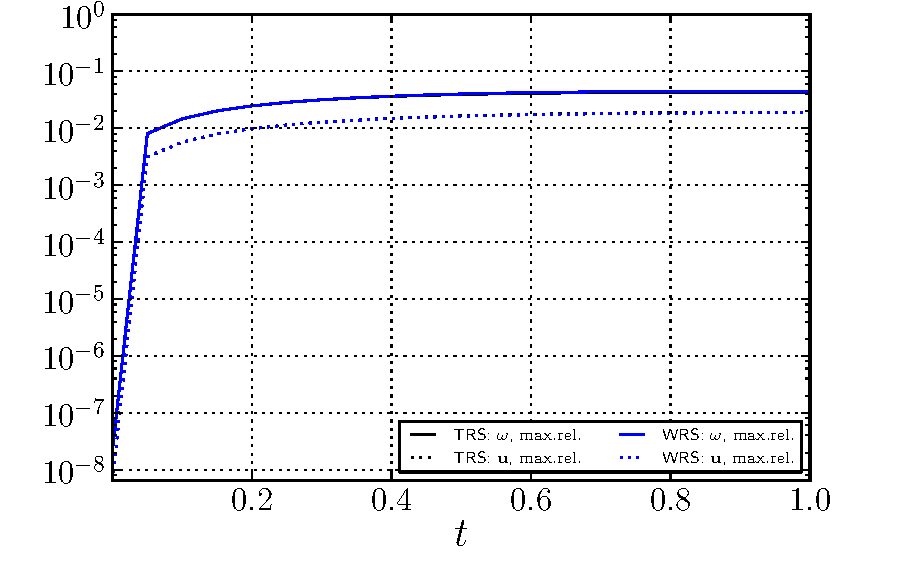
\includegraphics[width=\textwidth]{figures/lagrangian/lambOseen_errorEvolution_WRSvsTRS_dt0p05.pdf}
          \caption{$\Delta t_c = 0.05$}
          \label{fig:lambOseen_errorEvolution_WRSvsTRS_dt0p05}
  \end{subfigure}
  
  \caption{Comparison of Tutty's scheme TRS, and Wee-Ghoniem scheme WRS for treating diffusion, depicting the evolution of maximum relative error in vorticity, equation \ref{eq:maxRelErrorDef} from $t=0$ to $t=1$. The figure \textbf{(a)} shows TRS performing diffusion at every step, $\Delta t_d=\Delta t_c = 0.01$ and WRS performing diffusion at every $7^{\mathrm{th}}$ step, $\Delta t_d = k_d\cdot\Delta t_c = 7\times0.01$; \textbf{(b)} shows TRS performing diffusion at every step, $\Delta t_d=\Delta t_c = 0.05$ and WRS performing diffusion at every step, $\Delta t_d = k_d\cdot\Delta t_c = 1\times0.05$.}
  \label{fig:lambOseen_diffusionMethod_comparison}
 \end{figure}

However, when modifying the convective time step to $\Delta t_c=0.05$, figure \ref{fig:lambOseen_errorEvolution_WRSvsTRS_dt0p05}, we observe that the error of WRS matches the TRS. At this convective time step $\Delta t_c$, the WRS has a diffusion time step size $\Delta t_d = k_d \cdot \Delta t_c = 0.05$, where the diffusion frequency $k_d = 1$ now. Therefore, the WRS performs diffusion at every step and we see that WRS performs similarly to TRS.

The conclusion to this investigation is that WRS is useful if we are able to match the convective time step $\Delta t_c$ to the diffusion time step $\Delta t_d$. However, this may not be possible for high Reynolds number flows where the convective time step is critical. The TRS outperforms WRS in this regard and should produce less error when coupling with the Eulerian method.

%
%for both diffusion schemes. The solid lines represent the solution of the WRS, and the dashed lines shows the SRS. The convection and the diffusion time steps where controlled by modifying the blob spacing $h$, and keeping the convection time step size $\Delta t_c = 0.01$. 

	%	\begin{figure}[!h]
	%	\centering
	%	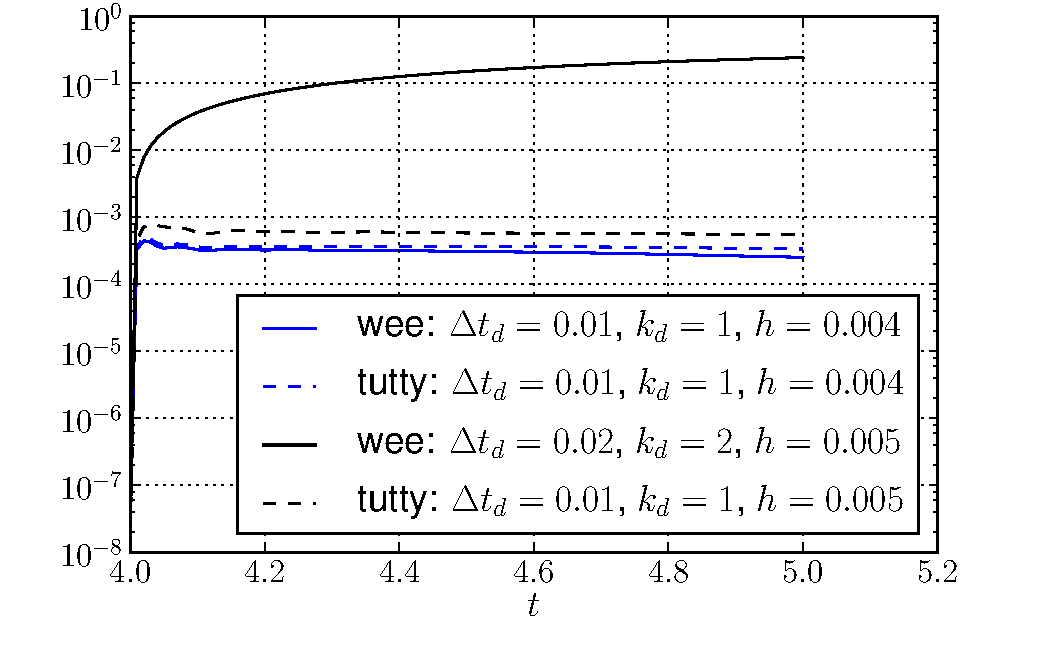
\includegraphics[width=0.6\textwidth]{figures/lagrangian/lambOseen_diffusionMethod_comparison_compressed.pdf}
	%	\caption{Comparison of Tutty's scheme TRS, and Wee-Ghoniem scheme WRS for treating diffusion. Figure depicts the growth in maximum relative error in vorticity, equation \ref{eq:maxRelErrorDef} from $t=0$ to $t=1$. 
	%	
	%	
	%	at $\Delta t_c = 0.01$. The Wee diffusion scheme with $\Delta t_d = \Delta t_c = 0.01$ [{\color{plotBlue}{---}}, solid blue], and $\Delta t_d = 2 \Delta t_c = 0.02$ [---, solid black]. The Tutty's diffusion scheme, $c^2 = 1/3$, with $\Delta t_d = \Delta t_c = 0.01$ [ {\color{plotBlue}{- -}}, dashed blue], and $\Delta t_d = \Delta t_c = 0.02$ [ - -, dashed black].}
	%	\label{fig:lambOseen_diffusionMethod_comparison_compressed}
	%	\end{figure}
	%	
	
  

%At $h = \num{4e-3}$, both schemes have the diffusion time step $\Delta t_d = 0.01$ meaning that the diffusion occurs at every iteration $k_d = 1$. During this time we see that the MRS performs slightly better that the SRS scheme. This is because, the diffusion of the vortex blobs is directly incorporated into the remeshing process, whereas the Tutty's SRS segregates the diffusion and the remeshing into two subsequent process. 

%At $h = \num{5e-3}$, the diffusion constraint on the Wee's MRS changes the minimum allowable diffusion time step to $\Delta t_d = 0.02$, meaning that diffusion has to be performs at every second step, $k_d=2$. Whereas for Tutty's SRS, we are not constraint by the minimum diffusion time step as so we can perform diffusion at $k_d = 1$. When investigating the growth in error for MRS, we see that the diffusion scheme has a large increase in the error, whereas the SRS does not have this limitation and is still able to diffuse at every step and has only a slight increase in error, figure \ref{fig:lambOseen_diffusionMethod_comparison_compressed} (solid black line). The diffusion scheme over-estimates the diffusion, and results in an incorrect diffusion process. However, we see that Tutty's SRS still performs a stable diffusion (dashed black line).

%This verification of the diffusion scheme showed that if Wee's MRS diffuses at $k_d > 1$, it will over-estimate the diffusion of the vorticity. Therefore, when using this scheme we will have to ensure that $k_d = 1$, by adjusting the convective time step appropriately. However, for large Reynolds number flows this is not possible, and so we must rely on the more stable and versatile Tutty's SRS diffusion scheme.

\subsection{Convergence study of the viscous vortex method}

Finally, we can perform a converge study, to validate that our scheme works according to the theory. For a scheme that is numerically stable, the error due to discretization must converge as the resolution of the discretization increases. 

	\begin{figure}[!b]
	        \centering
	        \begin{subfigure}[b]{0.5\textwidth}
	                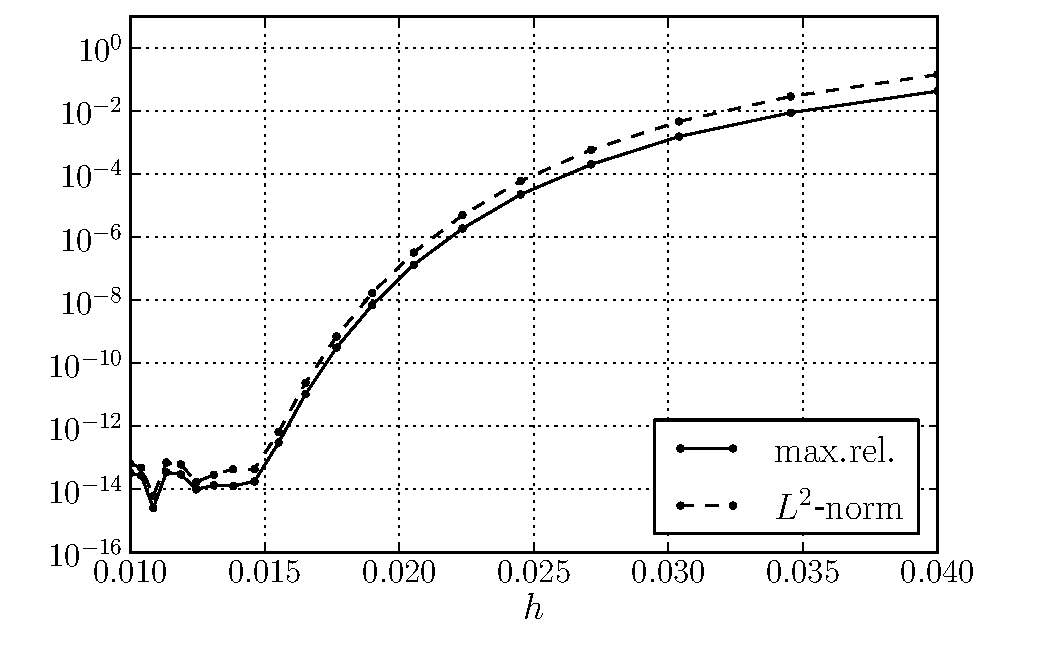
\includegraphics[width=\textwidth]{figures/lagrangian/lambOseen_convergence_dx_sigma0p02_compressed.pdf}
	                \caption{Error in vorticity vs. $h$ with $\sigma = 0.02$}
	                \label{fig:lambOseen_convergence_dx_sigma0p02_compressed}
	        \end{subfigure}%
	        ~ %add desired spacing between images, e. g. ~, \quad, \qquad etc.
	          %(or a blank line to force the subfigure onto a new line)
	        \begin{subfigure}[b]{0.5\textwidth}
	                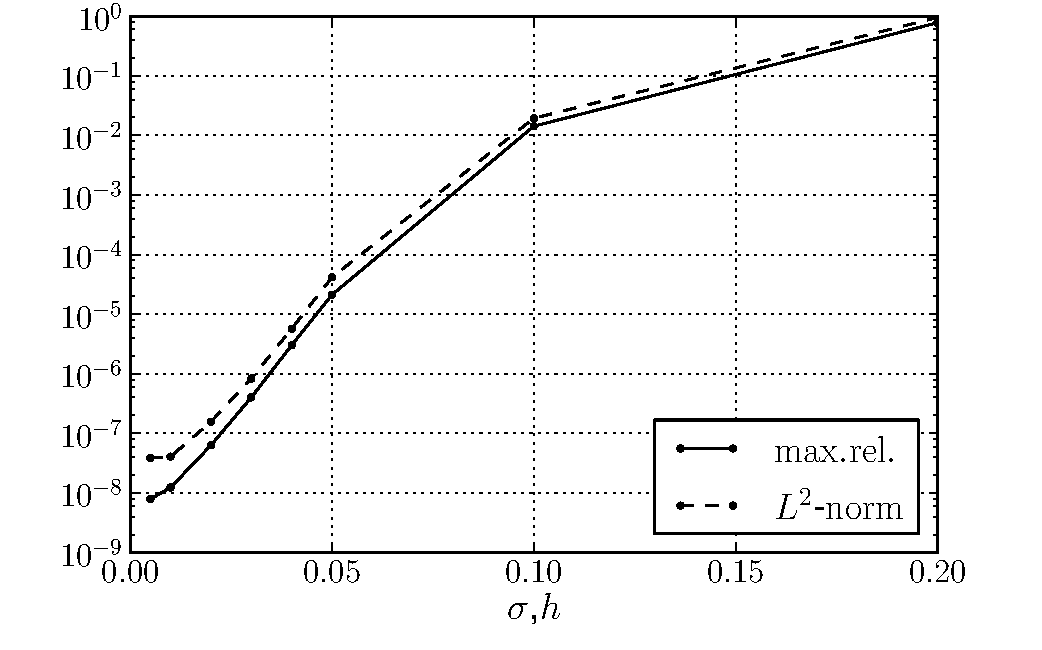
\includegraphics[width=\textwidth]{figures/lagrangian/lambOseen_convergence_dx_compressed.pdf}
	                \caption{Error in vorticity vs. $\sigma$, $h$ with $\lambda=h/\sigma=1$.}
	                \label{fig:lambOseen_convergence_dx_compressed}
	        \end{subfigure}
	        \caption{Convergence in spatial discretization of the vortex blobs. Figure \textbf{(a)} shows the convergence by fixing the core size $\sigma$ and \textbf{(b)} shows the convergence when overlap ratio $\lambda = h/\sigma = 1$.}
	        \label{fig:lambOseen_convergence_dx}
	\end{figure}

First, we investigate the convergence for spatial discretization. As we are dealing with vortex blobs, there are multiple ways of increasing the resolution. The straightforward method would be to increase the density of particles in a given area, i.e. reduce the blob spacing $h$ and maintaining the core spreading $\sigma$. Figure \ref{fig:lambOseen_convergence_dx_sigma0p02_compressed} shows the convergence of the spatial discretization when the core size $\sigma$ is maintained at $\sigma=0.02$. For this case, the overlap ratio changes with the blob spacing, described by equation \ref{eq:overlapRatio}. For small blob spacing $h$, the error in vorticity quickly drops to near machine precision. When investigating the order of convergence, we see that the error converges in a non-linear fashion and similar results have been obtained by Barba \cite{Barba2004c}.

Figure \ref{fig:lambOseen_convergence_dx_compressed}, shows the convergence of the error when the overlap ratio is fixed, $\lambda = 1$. In this test case, the core size scaled with the blob spacing, $h=\sigma$, and when increasing the spatial resolution, the error converges non-linearly.
	
	\begin{figure}[!h]
	\centering
	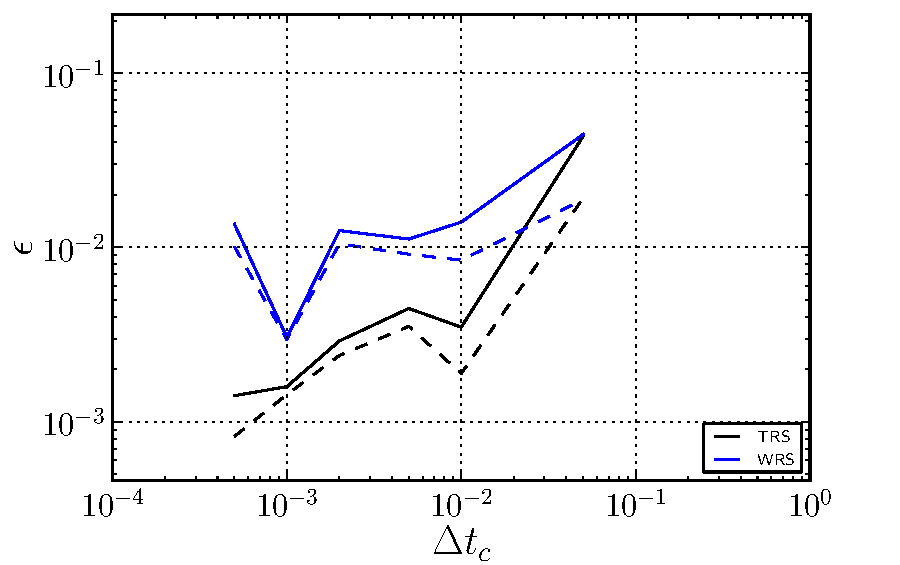
\includegraphics[width=0.6\textwidth]{figures/lagrangian/lambOseen_dtConvergence_WRSvsTRS.pdf}
	\caption{Convergence in temporal discretization of the vortex blobs. The Figure}
	\label{fig:lambOseen_dtConvergence_WRSvsTRS}
	\end{figure}	
	
To investigate the convergence in temporal discretization, we determined the evolution of the maximum relative error in vorticity, equation \ref{eq:maxRelErrorDef}, at $t=1$ for various convective time step sizes $\Delta t_c$, shown in figure \ref{fig:lambOseen_dtConvergence_WRSvsTRS}. At $t=1$, we see that the error reduces as we increase the temporal resolution meaning that we have a convergent scheme. We also observe that the error produced by WRS is higher than TRS and that it converges at a lower order than TRS. This again validates that TRS performs better than the WRS as it produces less error.


\section{Summary of the Lagrangian method}

In summary, we have investigated the Lagrangian domain of our hybrid method in this chapter. The Lagrangian method was used to described the evolution of the wake past the geometry. \printAcron{Vortex Particle Method}{VPM} was an ideal choice to describe the wake, as we require only to evolve the wake, and the generation of the vorticity is dealt with in the Eulerian domain. Unlike the Eulerian method, VPM only required the fluid elements where there was vorticity, meaning that the VPM was inherently auto-adaptive. Using the Population Control method, we were able to remove vortex blobs where they were not needed. Furthermore, the computation of the these elements were accelerated using an FMM, and simultaneously was parallelized using a GPU hardware. 

In section \ref{sec:introtovpm}, an introduction to the VPM was given. We determined advantage of the Lagrangian method w.r.t to the Eulerian method for resolving the wake for the VAWT. The velocity-vorticity formulation of the Navier-stokes equations is the governing equation of the VPM and we investigated the viscous splitting algorithm in section \ref{subsec:vsa}.

The viscous splitting algorithm enabled to perform diffusion and convection of the fluid is segregated steps. The discretization of the fluid through vortex blobs was investigated in section \ref{sec:spatialDiscretization}. These fluid elements has non-zero core size, removing the singularity when performing Biot-Savart calculations. 

In section \ref{subsec:vortexBlobInitialization}, we investigate the initialization of the vortex blobs. The proper initialization of the vortex blobs is a key factor for accurate coupling of Lagrangian method and the Eulerian method. The strengths of these particles is initialized by assigning the local circulation strength to the particle, as in equation \ref{eq:particleCirculationAssignment}. When the coupling is performed, it will be seen that the Gaussian blurring of the original vorticity field during the initialization is the fundamental source of error, section \ref{subsubsec:vfie}. Strategies such as Beale's iterative method, cannot be used as it is defined for an unbounded domain. The only approach found to minimize the Gaussian spreading initialization error is to increase the overlap ratio to $\lambda=1$, and minimize the blob spacing $h$ as much as possible, while keeping the computational effort to an acceptable level. The optimal strategy for the initialization of the vortex blob strengths is still an open question, and if solved can significantly improve the accuracy and the efficiency of the hybrid coupling

In section \ref{sec:covb}, we investigated the convection of the vortex blobs. The convection is performed using a $4^{\mathrm{th}}$-order Runge-Kutta time integration method. However, due to high strains in the fluid, the Lagrangian grid distortion of the vortex blob lattice has to be dealt with, section \ref{subsec:remeshing}. For this reason, we used a $\mathrm{M}'_4$ interpolation kernel that remeshed the particles onto a structured grid.

In section \ref{sec:diffusionVM}, we investigated two diffusion models for the vortex blobs. The WRS diffusion model developed by Wee and Ghonien \cite{Wee2006a}, integrated the diffusion process into the standard interpolation kernel.  This reduces computation cost, however the model was unfavourable constraint on the diffusion time step size, equation 
\ref{eq:la_dtcts}. The constraint limits the minimum diffusion step size and results in a discontinuous diffusion in time, as shown in figure \ref{fig:lambOseen_errorEvolution_WRSvsTRS_dt0p01}. To overcome this problem, we used the TRS diffusion model by Tutty \cite{Tutty2010a}, which enabled us to perform diffusion after every convection step, section
\ref{subsubsec:srs}. This also ensured that the diffusion process was continuous, which was important when performing the coupling algorithm.

In section \ref{sec:boundaryConditions}, we investigated the handling of the \emph{no-slip} boundary conditions for the viscous VPM. The boundary integral equations was used to enforces the wall boundary conditions in the Lagrangian method. We used the Constant-Strength Vortex panels, based on Katz \cite{Katz2001a}, to discretize the integral equations. The panel method was then verified and validated with the analytical solution of a potential flow around a cylinder in section \ref{sec:volm}. 

In section \ref{sec:volm}, we also verified and validated the implementation of the vortex blobs to analytical solution of the Lamb-Oseen vortex problem. We determined the evolution of the error for various spatial discretization and temporal discretization. The validation concluded that the implementation performed according to the literature, see example Barba \cite{Barba2004c}.



\section{Chapter Nomenclature}

{\textbf{\textsf{Latin Symbols}}}

{\renewcommand{\arraystretch}{1.2} %<- modify value to suit your needs
\begin{longtable}{p{1.5cm}p{10.5cm}p{1.5cm}}
    $\mathbf{A}$			& Vortex panel influence matrix						& -\\         

	$c^2$ 					& Diffusion parameter 								& - \\

    $\mathcal{E}$			& Enstrophy			  								& \si{m^2.s^{-2}} \\

	$f_{pc}$				& Population control frequency & - \\
	$f_{redis}$				& Redistribution frequency & - \\
	
    $h$						& Nominal particle spacing							& \si{m}\\   
    $h_{\nu}$				& Characteristic diffusion distance					& \si{m}\\ 

	$k$ & Gaussian kernel width spreading	& -\\
	$k_d$ & Frequency of vortex blob diffusion  								& -\\
    $\mathbf{K}$			& Biot-Savart kernel 								& -\\ 
    $\mathbf{K}_{\sigma}$	& Vortex blob kernel 								& -\\     

	$\hat{\mathbf{n}}$  	& Unit normal vector 								& -\\
	$N$  					& Number of vortex blobs (particles) 				& -\\

	$\lambda$			& Overlap ratio 									& - \\    
	
	$p$						& Pressure											& \si{Pa}\\

	$r$ 					& Radial position 									& \si{m}\\
	
	$\hat{\mathbf{s}}$		& Unit tangent vector								& - \\
	
	$t$						& Simulation time									& \si{s} \\
	
	$\mathbf{u}$			& Velocity 											& \si{m.s^{-1}}\\
	$\mathbf{u}_b$			& Velocity of the body 								& \si{m.s^{-1}}\\
	$\mathbf{u}_{\gamma}$	& Vortex sheet induced velocity                   	& \si{m.s^{-1}}\\	
	$\mathbf{u}_{\mathrm{ext}}$		& External induced velocity							& \si{m.s^{-1}}\\	
	$\mathbf{u}^h$			& Discrete velocity                               	& \si{m.s^{-1}}\\		
	$\mathbf{u}_{\infty}$	& Free-stream velocity								& \si{m.s^{-1}}\\			
	$\mathbf{u}_{\phi}$		& Free-stream velocity                            	& \si{m.s^{-1}}\\				
	$u_{r}$					& Radial velocity									& \si{m.s^{-1}}\\			
	$u_{\theta}$			& Angular velocity                               	& \si{m.s^{-1}}\\
	$\mathbf{u}_{\mathrm{slip}}$	& Boundary slip velocity					& \si{m.s^{-1}}\\
	$\mathbf{u}_{\omega}$	& Vorticity velocity 								& \si{m.s^{-1}}\\	

	$W$ 					& Interpolation kernel weight 						&-\\		
	$\mathbf{x}$			& Position vector 									& \si{m}\\		
	$\mathbf{x}_{\nu}$		& Position vector of particle to be diffused 		& \si{m}\\			
	$\mathbf{x}_{p}$		& Position vector of vortex blob (particle)			& \si{m}\\				
    %\caption{Attributes of \texttt{HybridSolver} class and their description.}
    %\label{tab:attributeHybrid}
\end{longtable}}

{\textbf{\textsf{Greek Symbols}}}

{\renewcommand{\arraystretch}{1.2} %<- modify value to suit your needs
\begin{longtable}{p{1.5cm}p{10.5cm}p{1.5cm}}
	$\alpha_p$ 		& Circulation of the particle & \si{m^2.s^{-1}}\\
	%$\beta_p$ 		& Corrected circulation of the particle & \si{m^2.s^{-1}}\\	

	$\Delta t_c$ 		& Convection time step size & \si{s}\\
	$\Delta t_d$ 		& Diffusion time step size & \si{s}\\	

	$\epsilon$ 		& Relative error & -\\		

	$\Gamma$ 		& Circulation & \si{m^2.s^{-1}}\\	
	$\Gamma_{glob}$ 		& Particle circulation threshold & \si{m^2.s^{-1}}\\	
	$\Gamma_{glob}$ 		& Total circulation threshold & \si{m^2.s^{-1}}\\		
	%$\Gamma_b$ 		& Circulation inside a moving body & \si{m^2.s^{-1}}\\		
	%$\gamma_c$ 		& Vortex sheet strength & \si{m^2.s^{-1}}\\			
	%$\Gamma_{\gamma}$ 	& Circulation of the vortex sheet & \si{m^2.s^{-1}}\\				
	%$\gamma_{\omega}$ 	& Circulation of the fluid & \si{m^2.s^{-1}}\\					

	$\nu$ & Kinematic viscosity & \si{m^2.s^{-1}}\\

	$\omega$ & Vorticity & \si{s^{-1}}\\
	$\tilde{\omega}$ & Vortex blob cell vorticity & \si{s^{-1}}\\
	$\omega^h$ & Discrete vorticity field & \si{s^{-1}}\\

	$\Omega$ & Fluid domain & \si{m}\\

	$\rho$ & Density & \si{kg.m^{-3}}\\
	
	$\sigma$ & Core size & \si{m}\\
	$\tau$ & Lamb-Oseen time constant & \si{s}\\
	$\xi$ & Scale relative position of particle to stencil node & -\\
	$\zeta_{\sigma}$		& Smooth cut-off function of the blobs & -\\			

\end{longtable}}



	% Chapter 4: Eulerian Subdomain: Finite Element Method
	\chapter{Eulerian Method: Finite Element Method}
\label{ch:eulerian}

%	\lsymb[f]{$\mathcal{T}_h$}{Finite Element mesh}{-}{th}		
%	\lsymb[f]{$T$}{Cell of Finite Element mesh}{-}{t}			
%	
%	\lsymb[f]{$v$}{Test function}{-}{v}				
%	\lsymb[f]{$V$}{Trial vector function space}{-}{vte}				
%	\lsymb[f]{$\hat{V}$}{Test vector function space}{-}{vtr}					
%	\gsymb[f]{$\Omega$}{Fluid domain}{-}{x}	
%	\gsymb[f]{$\Omega_E$}{Eulerian fluid domain}{-}{xe}	
%	\gsymb[f]{$\Omega_L$}{Lagrangian fluid domain}{-}{xl}	
%	\gsymb[f]{$\partial \Omega$}{Boundary of the domain $\Omega$}{-}{xdd}	

%------------------------------------------------------------------------------------------------------
%------------------------------------------------------------------------------------------------------
%------------------------------------------------------------------------------------------------------
%\section{Purpose of eulerian domain}
Standard \printAcron{Computation Fluid Dynamics}{CFD} methods discretize the fluid into smaller grids, and solve the set of Navier-Stokes equations in these region. Eulerian methods uses this type of formulation.
%is referred to as an Eulerian , as we are evaluating the change of flow property in a given volume.

For the hybrid method, we use the Navier-Stokes Eulerian formulation in the near-body region. The advantage of using this formulation in this region is that it is much more efficient in resolving boundary layers than the \printAcron{Vortex Particle Method}{VPM}. We can directly enforce the wall boundary condition at the wall boundary of the Eulerian subdomain, solving the problem of vorticity generation of the body. %In the hybrid coupling strategy, we can then interpolate this newly resolved near-wall solution onto the Lagrangian domain, where the vortex blobs can efficiently evolve the particles.

The most common approaches to solve the fluid dynamics problem on an Eulerian reference frame are \indexAcron{Finite Volume Method }{FVM}, \indexAcron{Finite Difference Method}{FDM}, and \indexAcron{Finite Element Method}{FEM}. FVM divides the domain into volumes where it enforces the conservation of mass and momentum in each grid. FDM divides the domain into nodes and uses local Taylor expansions to approximate the partial differential equations. FEM divides the domain into elements and solves the problem using variational calculus. %So in the end, the choice of Eulerian method does not have a direct impact on the coupling with the Lagrangian method as the purpose of the Eulerian method is only to efficiently, and accurately resolve the near-body region of the body.

For the current study, we have decided to use the FEM package provided by the \fenics project as it has implemented efficient, multi-threaded algorithms for setting up and solve a finite element problem. Furthermore, it provides extensive features for future developments such as adaptive mesh refinement, deformable meshes, and efficient computation of turbulent flow.

\section{Introduction to the Finite Element Method}
\label{sec:e-ithfem}
The \printAcron{Finite Element Method}{FEM} is a numerical method to obtain approximations to partial differential equations. The equations are solved by writing them as a variational problem, giving us an approximate solution for the boundary value problem \cite{Brenner2002}. Therefore the FEM approximates the unknown functions and converts the partial differential equations into a set of algebraic equations, which makes them suitable to be solved numerically. It was traditionally used for solid mechanics (e.g for the analysis of aircraft structures \cite{RAO2011}), but have since been used to solve fluid dynamics problems \cite{Guermond2006a,Johnston2004a,Guermond2003a}.

%\cite{Guermond2006a} \cite{Johnston2004a} \cite{Guermond2003a}.

\subsection{Finite Element Discretization}

The finite element method solves a problem by dividing the domain of interest into smaller cells known as \textit{elements}. These \textit{elements} are connected at the vertices which are called nodes or nodal points. We use these sets of nodes and elements to represent the variation in the field such as the displacement, the velocity, the pressure or the temperature using simple functions, known as basis functions. Thus, we have transformed the problem of interest into a finite number of \indexAcron{Degrees of Freedom}{DOF}. We combined the set of equations of the elements into a global system of equations to solve for the unknowns.

	\begin{figure}[!h]
	\centering
	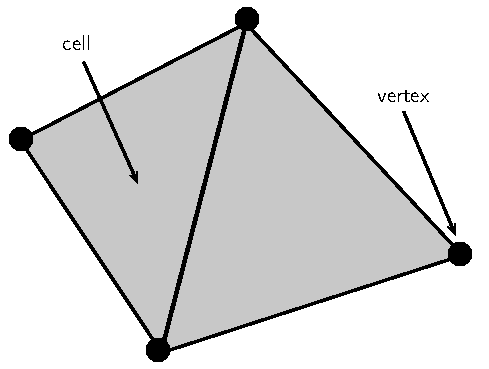
\includegraphics[width=0.4\linewidth]{./figures/eulerian/finiteElementDefinitions.pdf}
	\caption{A two-dimensional finite element geometry. The cell represents the area of the element, and vertices are the edges of the cell.}
	\label{fig:finiteElementDefinitions}
	\end{figure}

	\begin{figure}[!b]
	        \centering
	        \begin{subfigure}[b]{0.45\textwidth}
	                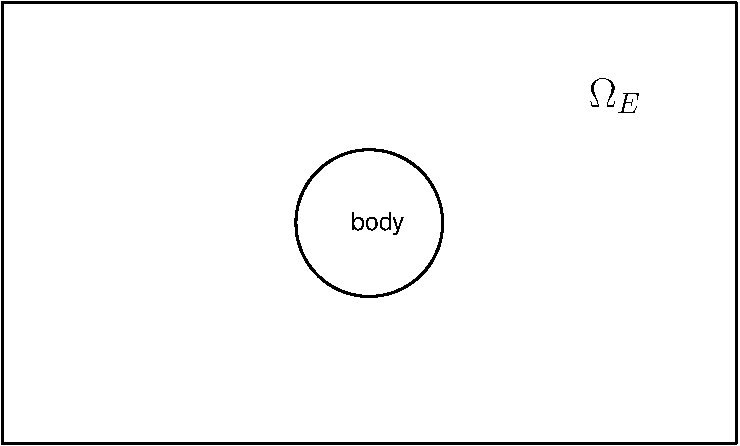
\includegraphics[width=\textwidth]{figures/eulerian/cylinderPreDelauney-crop.pdf}
	                \caption{Fluid domain $\Omega_E$ around the cylinder}
	                \label{fig:cylinderPreDelauney}
	        \end{subfigure}%
	        \qquad %add desired spacing between images, e. g. ~, \quad, \qquad etc.
	          %(or a blank line to force the subfigure onto a new line)
	        \begin{subfigure}[b]{0.45\textwidth}
	                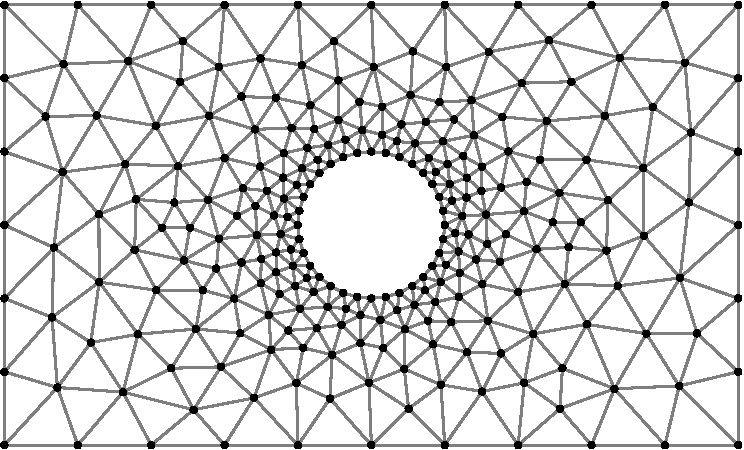
\includegraphics[width=\textwidth]{figures/eulerian/cylinderDelauney-crop.pdf}
	                \caption{Delaunay triangulation of the fluid}
	                \label{fig:cylinderDelauney}
	        \end{subfigure}
	        \caption{Delaunay triangulation of the fluid around a cylinder resulting in unstructured mesh with controllable cell sizes.}
	        \label{fig:cylinderFiniteElementDiscretization}
	\end{figure}	

A finite element discretization in 2D can be seen in Figure \ref{fig:finiteElementDefinitions}. The figure shows two connected elements, where the cells represent the area of the element, and the vertices of the cell represents the nodes of the element. The set of all the cells $\mathcal{T}_h = \{T\}$ in the fluid domain $\Omega$, constitutes the mesh of the Eulerian domain. In Figure \ref{fig:finiteElementDefinitions}, the cells of the finite element in 2D, are made of simple triangles. There are two approaches to discretize the domain: structured or unstructured meshes. The structured mesh has cells oriented in a pattern, and is the simplest approach to construct the mesh. The advantage of such a discretization is that it is possible to make a simple data structure which can be used to perform efficient computations. The downside to such discretization is that it is very difficult to construct structured mesh in complex domains with several holes. However, the FEM enables us to perform an unstructured discretization of the domain, as shown in Figure \ref{fig:cylinderFiniteElementDiscretization}. The figure shows the unstructured discretization of the fluid domain around the cylinder $\Omega_E$, connecting the rectangular outer boundary of the fluid to the circular no-slip boundary of the body in a simple fashion. Although the unstructured approach gives rise to less efficient discretization, its geometrical flexibility has advantages that surpasses the disadvantage.%This shows that even though the unstructured method formulation is more complicated that the structured formulation, we have the advantage that the mesh quality does not deteriorate as the domain becomes more complex.

There are several algorithms for mesh generation. The standard approach is to employ the Delaunay triangulation method derived from the Voronoi diagram concept \cite{Carey1997}. This divides the domain into a set of triangles, as shown in Figure \ref{fig:cylinderFiniteElementDiscretization}. This type of mesh generation allows us to connect boundaries with difference shapes together. %Furthermore, this triangulation method canbe controlled by predefining the boundary element nodes using a transfinite interpolation.

\subsection{Finite Element Functions and Function Spaces}

The finite element is defined using a triplet ($T, \mathcal{V}, \mathcal{L}$), as defined in Ciarlet \cite{Ciarlet1972b} and used in the \fenics Project \cite{Logg2012b}. $T$ is a tessellation of the domain $\Omega$, the space $\mathcal{V} = \mathcal{V}(T)$ is a finite dimensional function space on $T$ of dimension $n$, and $\mathcal{L} = \left\{ \ell_1,\ell_2,...,\ell_n \right\}$ is the set of degrees of freedom forming the basis for the dual space $\mathcal{V}'$ of $\mathcal{V}$.

Once we perform the tessellation, we can define the functions and the function spaces of the finite element problem. For each cell, a local function space $\mathcal{V}$ can be defined to collectively construct the global function space $V$. Any given function $u \in V$ is expressed as a linear combination of basis functions $\{\phi_1,\phi_2,...,\phi_N\}$,  of the function space $V$, 
	\begin{equation}
	u(x) = \sum_{j=1}^N U_j\phi_j(x).
	\end{equation}

There are several types of finite element families: the Brezzi-Douglas-Marini, the Crouzeiz-Raviart, the Discontinuous Lagrange, the Hermite, and the Lagrange elements \cite{Logg2012b}. For the current study, we will rely on the Lagrange elements, also known as the \indexAcron{Continuous Galerkin}{CG}, which are based on the Lagrange polynomials \cite{Chen2011}. These elements are widely used and are the simplest to implement for our project. 

%Each has its own advantage such as the Discontinous Lagrange, or \indexAcron{Discontinous Galerkin}{DG} element consists of discontinuous functions, which was originally introduced for solving hyperbolic problem by Reed and Hill in 1973 \cite{Reed1973a}. The method was able to conserve mass at each element, had a high-order accuracy, and was robust in solving the advection problem. However for the current problem, we will rely on the Lagrange elements, also known as the \indexAcron{Continuous Galerkin}{CG}, which are based on the Lagrange polynomials \cite{Chen2011}. These elements are widely used and are the simplest to implement for our project. 

Lagrange elements belong to the space $H^1$, which is a Sobolev space containing functions $u$ such that $u^2$ and $\left|\nabla u\right|^2$ have finite integral in the domain $\Omega$ \cite{Logg2012b}. The Lagrange element uses point evaluation for the degrees of freedom, where a DOF in $(x_i,y_i)$ denotes the point evaluation of the function $u$, $\ell_i(u) = u(x_i,y_i)$. We can have Lagrange elements of various orders $q = 1, 2,...$, where $q$ is the degree of the Lagrange polynomial $\mathcal{P}_q$. For the 2D case, the dimension $n$ of the finite element is given as,
	\begin{equation}
	n(q) = \frac{1}{2}(q + 1)(q + 2).
	\end{equation}

For $q=1$, we have a simple linear Lagrange element $\mathrm{CG}_1$ or linear interpolant with $3$ DOFs, known as the Courant triange \cite{Courant1943}. For a higher order finite element, we can set $q=2$, giving us a Lagrange element $\mathrm{CG}_2$ with $6$ DOFs per cell. Figure \ref{fig:continuousGalerkin} shows the two Lagrange triangles $\mathrm{CG}_1$ and $\mathrm{CG}_2$ for $q = 1$ and $q=2$ respectively. The Courant triangle has the DOFs located at the vertices of the cell, and the higher order $\mathrm{CG}_2$ has $3$ additional DOFs, all located midway between the vertices. Our Eulerian method of our hybrid scheme, is based on the $\mathrm{CG}_1$ and $\mathrm{CG}_2$ Lagrange elements.

	\begin{figure}[t]
	\centering
	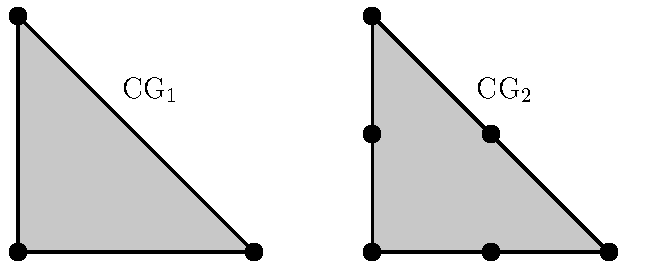
\includegraphics[width=0.6\linewidth]{./figures/eulerian/continuousGalerkin.pdf}
	\caption{The Lagrange $\mathrm{CG}_q$ triangle for $q = 1, 2$. The triangles have $3$ and $6$ DOFs respectively ({\color{black}{$\bullet$}}, black dot).}
	\label{fig:continuousGalerkin}
	\end{figure}



\subsection*{Variational Formulation}
\label{subsec:variationalProblem}

To solve a problem such as the Poisson equation numerically with FE, we need to convert it into a variational problem. The methodology is followed from the \fenics tutorial provided by Langtangen \cite{Logg2012b}. A 1D Poisson problem is given as,
	\begin{equation}
	\begin{aligned}
	- \nabla^2 u(x) &= f(x), \qquad x\ \mathrm{in}\ \Omega,\\
	u(x) &= u_0(x), \qquad x\ \mathrm{on}\ \partial\Omega.
	\end{aligned}
	\label{eq:poissonEq}
	\end{equation}
	
We can transform equation \ref{eq:poissonEq} into a variational form by multiplying it with a test function $v$, and integrating it over the domain $\Omega$,
	\begin{equation}
	- \int_{\Omega} \left(\nabla^2 u\right)v\ \mathrm{d}x= \int_{\Omega} fv\ \mathrm{d}x, \qquad \forall\ v \in \hat{V}.
	\label{eq:poissonEqVariationFormA}
	\end{equation}

In equation \ref{eq:poissonEqVariationFormA}, the function $u$ is the trial function, and is what we are trying to approximate. The trial function $u$ lies in the trial function space $V$, and the test function $v$ lies in the test function space $\hat{V}$. When performing integration by parts, the test function $v$ is required to be zero at regions where $u$ is known. So, the additional terms cancel and we get,
	\begin{equation}
	- \int_{\Omega} \nabla u \nabla v\ \mathrm{d}x= \int_{\Omega} fv\ \mathrm{d}x \qquad \forall\ v \in \hat{V}
	\label{eq:poissonEqVariationFormB}
	\end{equation}

This form is referred to as the \textit{weak-form} of the original Poisson equation and is valid for all $v$ in the trial space $\hat{V}$. An inner product of any two functions $f$ and $g$ in domain $\Omega$ is defined as,
	\begin{equation}
	\langle f,g \rangle = \int_{\Omega}fg\ \mathrm{d}x,
	\label{eq:innerProductRule}
	\end{equation}
so we can rewrite equation \ref{eq:poissonEqVariationFormB} as,
	\begin{equation}
	-\langle \nabla u,\nabla v \rangle = \langle f,v \rangle, \qquad \forall\ v \in \hat{V}.
	\end{equation}

In order to solve this continuous problem numerically, we must transform it into a discrete variational problem,
	\begin{equation}
	-\langle \nabla u_h, \nabla v \rangle = \langle f, v \rangle \qquad \forall\ v \in \hat{V}_h \subset \hat{V},
	\label{eq:poissonEqDiscreteVariational}
	\end{equation}
where $u_h$ is the approximate solution function belonging to the discrete function in the discrete space $V_h$ which is a subset of $V$. Similarly the test discrete function space $\hat{V}_h$ is a subset of $\hat{V}$. The linear triangular element, shown in Figure \ref{fig:continuousGalerkin} is used as the function space, where $\hat{V}_h$ and $V_h$ are described by piecewise linear functions of the triangle. At the boundary, the functions in the test space are zero, whereas the functions in the trial space are equal to the boundary condition $u_0$. In the Langtangen \cite{Logg2012b}, $u$ is used to denote/write the solution of the discrete problem, ignoring the subscript $h$ of $u_h$. Therefore, to have a one-to-one relation with literature, we will employ the same notation from here on. The equation \ref{eq:poissonEqDiscreteVariational} can be simplified as,
	\begin{equation}
	a\left(u,v\right) = L(v),
	\label{eq:weakForm}
	\end{equation}
where,
	\begin{equation}
	a\left(u,v\right) = - \langle \nabla u, \nabla v \rangle,
	\end{equation}
and
	\begin{equation}
	L(v) = \langle f,v \rangle.
	\end{equation}

The variable $a(u,v)$ and $L(v)$ is the denoted as the bilinear and linear form, respectively. Since, $u\in V$, it can be written as a linear combination of the basis functions $\{\phi_i,...,\phi_N\}$ of $V$, with $\mathrm{span}\{\phi_i,...\phi_N\}=V$, we can express $u$ as,
	\begin{equation}
	u = \sum_{j=1}^{N} U_j \phi_j.
	\label{eq:trialDiscrete}
	\end{equation}
Similarly, the test function $v$ can be written as linear combination of basis functions $\{\hat{\phi}_i,...,\hat{\phi}_N\}$, with $\mathrm{span}\{\hat{\phi}_i,...,\hat{\phi}_N\}=\hat{V}$, 
	\begin{equation}
	v=\sum_{i=1}^{N} V_i \hat{\phi}_i.
	\label{eq:testDiscrete}
	\end{equation}
		
Since equation \ref{eq:weakForm} has to valid for all $v \in \hat{V}$, and $\hat{V}$ can be written as a linear combination of the basis functions, equation \ref{eq:weakForm} must be valid for each of the basis functions. Therefore, equation \ref{eq:weakForm} can be expressed as, 

	\begin{equation}
	a(\sum_{j=1}^N \ U_j \phi_j,\hat{\phi}_i) = L(\hat{\phi}_i), \qquad \forall\ \phi_i, i = 1,...,N.
	\end{equation}

and simplifies to,	
	\begin{equation}
	\sum_{j=1}^N U_j a(\phi_j,\hat{\phi}_i) = L(\hat{\phi}_i), \qquad \forall\ \phi_i, i = 1,...,N.
	\end{equation}
This is an algebraic system of equations:
	\begin{equation}
	\mathbf{A}U = b,
	\label{eq:linearSysOfEq}
	\end{equation}	
where $\mathbf{A}_{ij} = a(\phi_j,\hat{\phi}_i)$ and the \printAcron{Right-Hand Side}{RHS} $b_i$ is given by $b_i=L(\hat{\phi}_i)$.
 	
\section{Solving the Finite Element Problem}
\label{sec:e-stfep}

To solve the finite element problem, we used \dolfin, the finite element library of the \fenics Project. This library uses high performance linear algebra kernels, and provide a scripting interface to \textsc{Python}. The Python scripting environment helps us to focus on the development of the theory (i.e the high-level algorithms). In order to generate the mesh of the fluid domain, we used \textsc{Gmsh}, a three-dimensional finite element mesh generator which proves a fast, light and user-friendly meshing tool.

\subsection{Introduction to FEniCS Project}

The \fenics Project is a collaborative work of various universities that developed tools to perform automated finite element algorithms, which can be used to solve partial differential equations. It was a project originated in 2003 with the research collaboration of University of Chicago and Chalmers University of Technology from Logg,  Mardal, and Wells \cite{Logg2012b}. Since then, several other groups have joined such as the Royal Institute of Technology, Simula Research Laboratory, University of Cambridge and Delft University of Technology.

	\begin{figure}[!h]
	\centering
	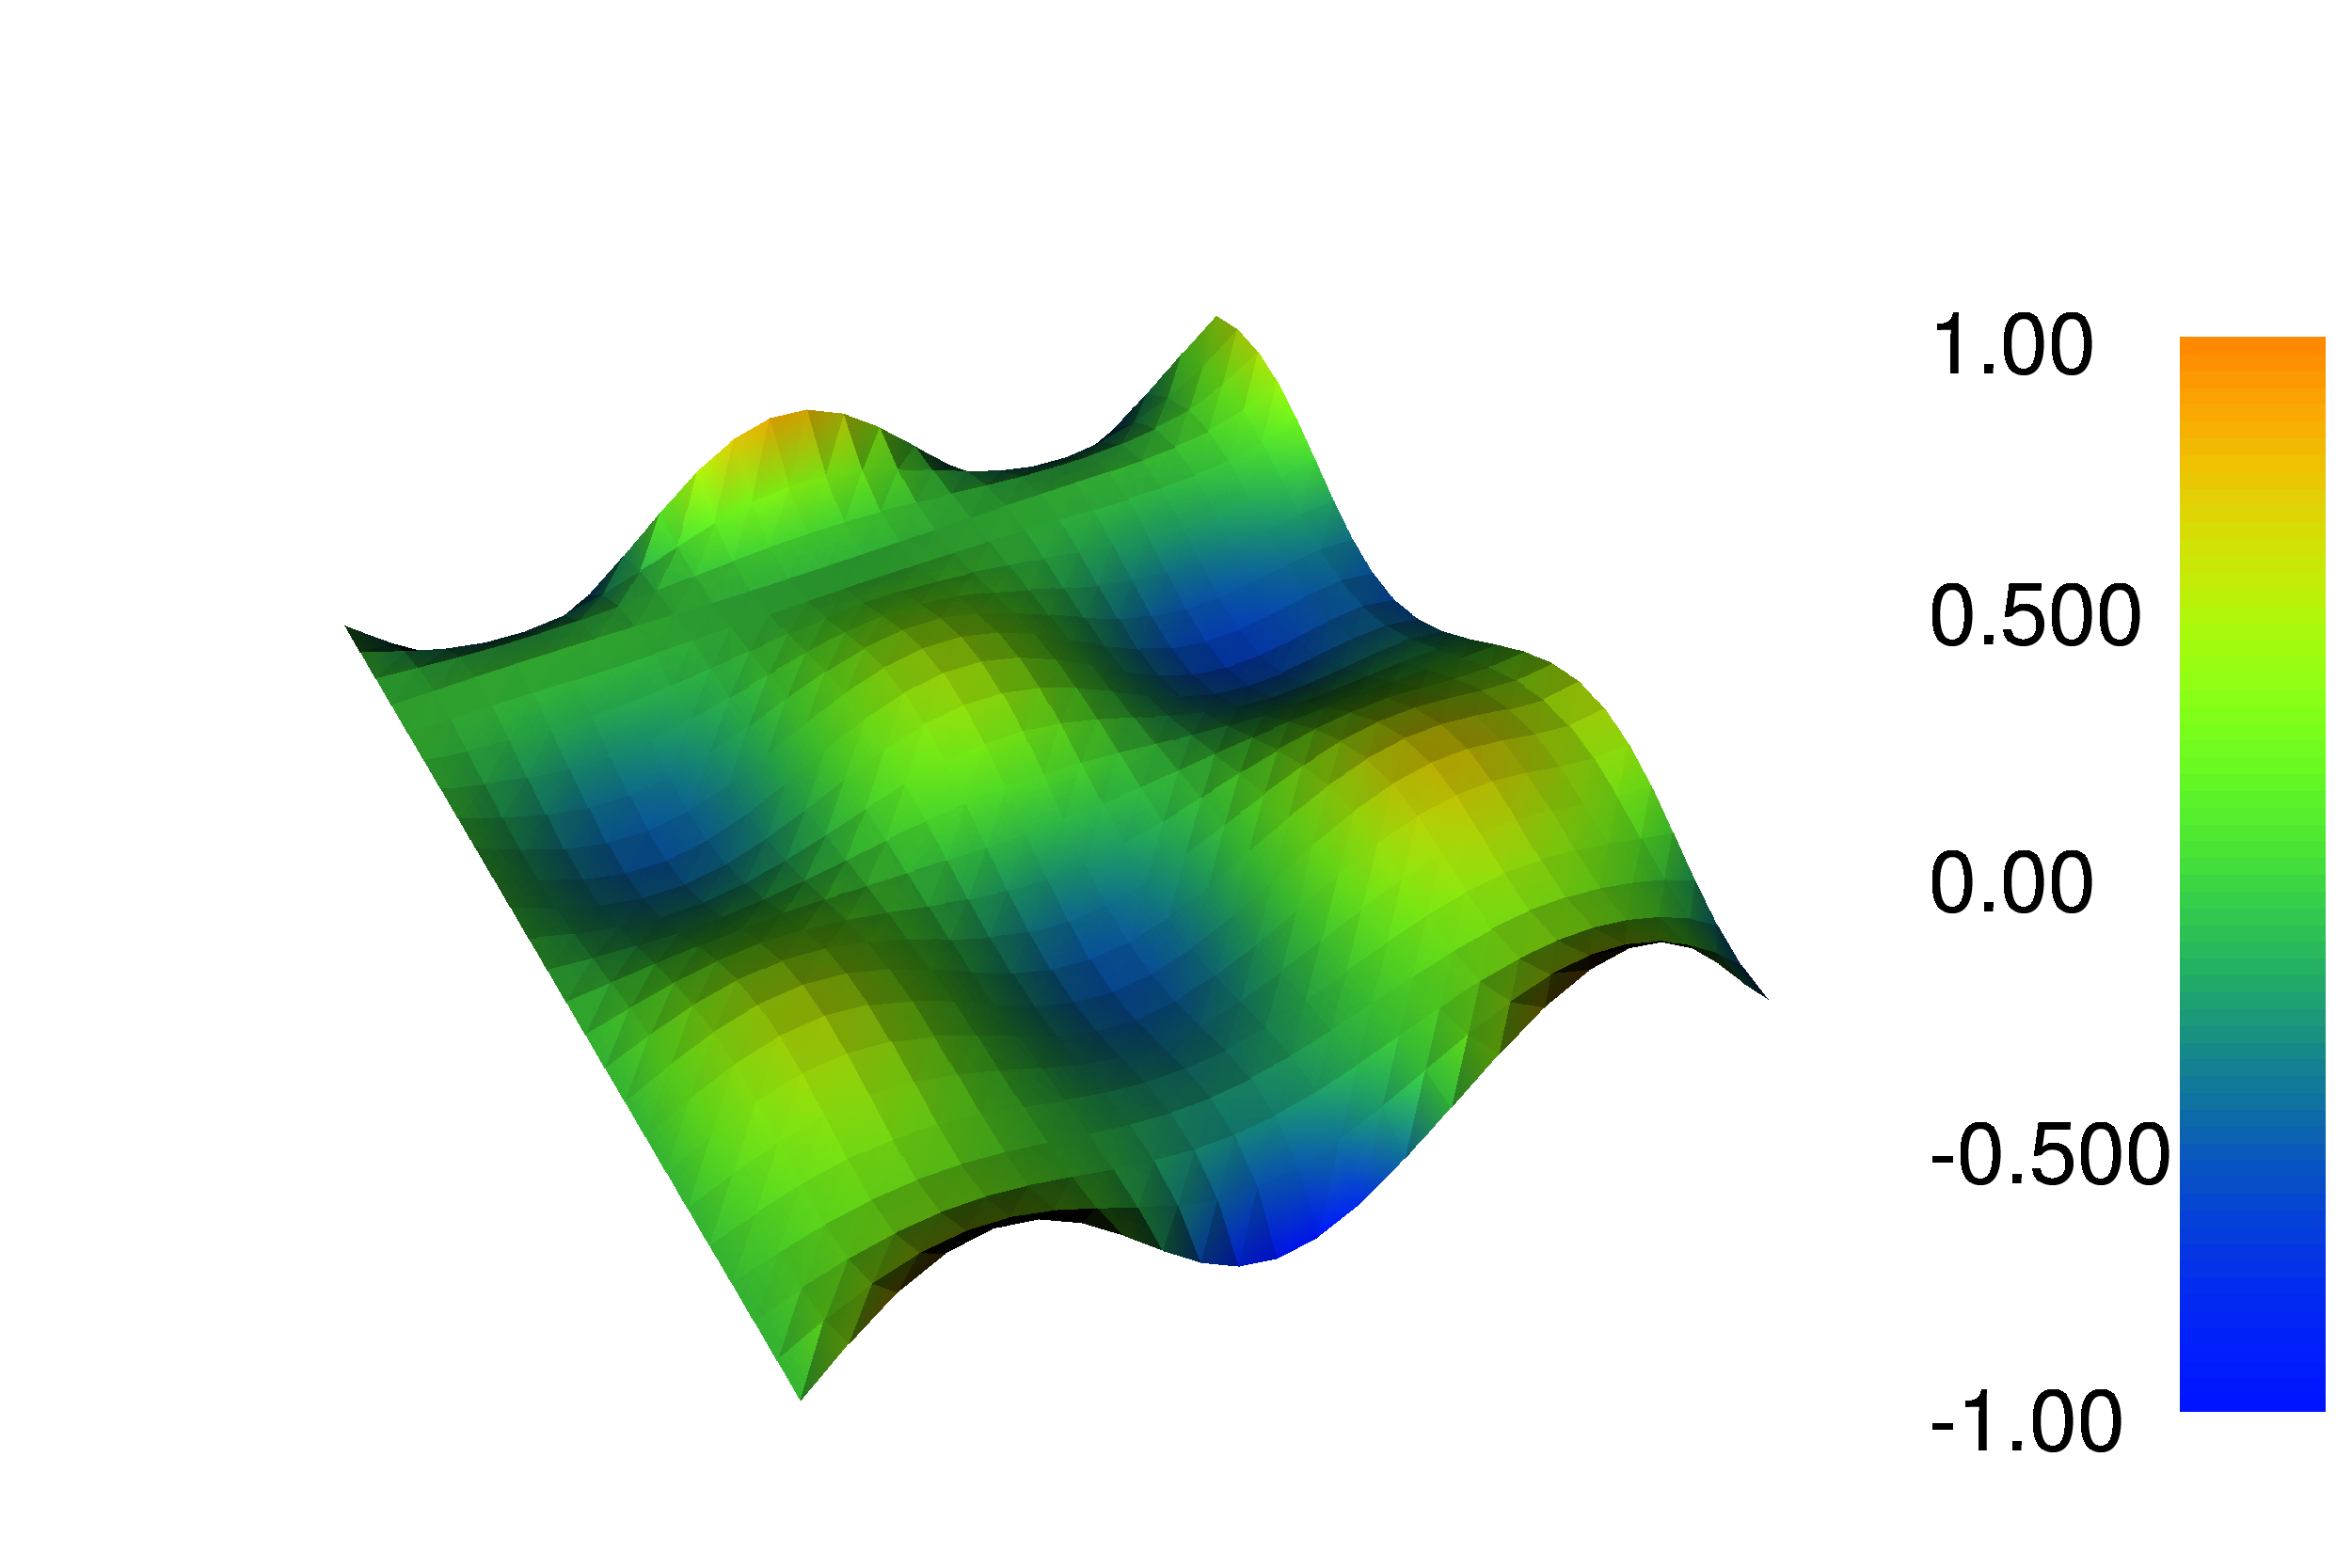
\includegraphics[width=0.5\linewidth]{./figures/eulerian/dolfin_plot_2-rotated270.png}
	\caption{\dolfin VTK plot of the Poisson solution, given by the problem, source code listing \ref{lst:pycode-poisson}.}
	\label{fig:dolfinExampleFigure}
	\end{figure}

\fenics consists of various libraries such as UFC, UFL, FIAT, INSTANT and \textsc{Dolfin}. \dolfin is the core library aimed at automating the solution of partial differential equations using the finite element method \cite{Logg2010a}. It uses automated code generation thus maintaining high-level mathematical expressions but still providing efficient, multi-threaded performance (with \indexAcron{Message Passing Interface}{MPI}) internally. %It used built-in linear algebra backend such as PETSc, TRILINOS/EPECTRA, uBLAS, and MTL4.

We used the \dolfin library wrapped in \python to set up and solve the finite element problem. For example, we can demonstrate the procedures of solving the Poisson problem, equation \ref{eq:poissonEq}. We can take $f=2\cdot\sin{x}\cdot\cos{y}$ with the boundary conditions,
	\begin{equation}
	u(x) = u_0(x) = \sin x \cdot \cos y, \qquad (x,y) \in \partial\Omega.
	\end{equation}
The finite element code generation is automated with \textsc{Dolfin}, leaving only the explicit expression of the problem in python, see source code listing \ref{lst:pycode-poisson}. Figure \ref{fig:dolfinExampleFigure} shows the VTK plot of the solution for the Poisson problem.

	\begin{listing}[p]
	\inputminted[fontseries=courier,obeytabs,fontsize=\footnotesize,mathescape,linenos,numbersep=5pt,frame=lines,framesep=2mm,xleftmargin=20mm,xrightmargin=20mm]{python}{figures/eulerian/dolfinExample.py}
	\caption{A complete program for solving the Poisson problem and plotting the solution. The Poisson problem is given as $-\nabla^2{u} = f$, where $u_0 = \sin{x}\cdot\cos{y}$ on the boundary and $f=2\cdot\sin(x)\cdot\cos(y)$. The code is written in \python using \dolfin 1.2 library}
	\label{lst:pycode-poisson}
	\end{listing}

\subsection{Mesh Generation using GMSH}
\label{subsec:mgugmsh}
%The proper generation of the fluid mesh is an important aspect of the Finite Element method. It is an important process, as an ill-construct mesh can be computationally very expensive, or might even problem with convergence. There have been literatures dedicated just to improve the mesh generation, for example by Hansen \cite{Hansen2005}. It focused on mesh enhancement techniques for elliptical methods, which enables to increase the quality of the data, and also the robustness of the simulation.

The generation of the mesh is achieved by \textsc{Gmsh}, an open-source software developed by Geuzaine \& Remacle \cite{Geuzaine2009b}, which has implemented a user-friendly interface and fast algorithms. The \gmsh implemented kernels use \textsc{BLAS} and LAPACK linear algebra packages in C++ for fast computation. Furthermore, it allows for scriptability making it ideal to integrate it with our current \python code project for future automation.

\section{Solving Incompressible Navier-Stokes Equations}
\label{sec:e-sinse}

Using the \dolfin library for constructing the finite element problem, we can now solve the flow in the Eulerian subdomain of our hybrid scheme. The Eulerian method use the primitive variables velocity-pressure $\mathbf{u}-p$ to describe the flow.

\subsection{Velocity-Pressure Formulation}
The velocity-pressure $\mathbf{u}-p$ formulation of the fluid flow problem, is the standard formulation of the Navier-Stokes equations. The 2D incompressible Navier-Stokes equations of a fluid with unit density (i.e $\rho = 1$) is given as,
	\begin{subequations}
	\begin{align}
	\frac{\partial \mathbf{u}}{\partial t} + \mathbf{u}\cdot\nabla\mathbf{u} - \nabla \cdot \sigma &= f,\\
	\nabla \cdot \mathbf{u} = 0,
	\end{align}	
	\label{eq:2Dns}
	\end{subequations}
where $\sigma$ is the Cauchy stress tensor defined as,
	\begin{equation}
	\sigma(\mathbf{u},p) = 2\nu\epsilon(\mathbf{u}) - p\mathbf{I}.
	\label{eq:stressTensor}
	\end{equation}

The Cauchy stress tensor is a function of pressure $p$, the fluid kinematic viscosity $\nu$, and the symmetric gradient $\epsilon$ defined as,
	\begin{equation}
	\epsilon(\mathbf{u}) = \frac{1}{2} \left(\nabla \mathbf{u} + \nabla \mathbf{u}^{\mathrm{T}}\right).
	\label{eq:symGrad}
	\end{equation}
describing the stresses in the fluid due to the velocity gradient and the pressure. The incompressible 2D Navier-Stokes equations have two unknowns, the vector velocity field $\mathbf{u}$, that lies on the vector-valued function space $V$, and the scalar pressure field $p$, which lies on the scalar-valued function space $Q$. Once we compute these two quantities we can determine the vorticity field, which we then transfer to the Lagrangian subdomain. 

\subsection{Determining the Vorticity Field}
\label{subsec:dtvf}

The coupling between the Eulerian and the Lagrangian subdomain is done by transferring the vorticity field $\omega$ from the Eulerian subdomain to the Lagrangian vortex blobs. The vorticity field $\omega$, is defined as:
	\begin{equation}
	\omega = \nabla \times u,
	\label{eq:vorticityEq}
	\end{equation}
where the vorticity $\omega$ lies on the scalar-valued function space $X$. However, as $\nabla\times\mathbf{u}\notin{X}$, because $\mathbf{u}\in V$, we require a projection from the velocity function space $V$ onto the vorticity function space $X$. In variational formulation, this requires the following equality to be satisfied,
%Due to the constant change in the velocity field, we have to recalculate the vorticity at every time step $t_n, t_{n+1}, ...$ . To solve this problem in an efficient manner, we can use the \texttt{assemble} function of \dolfin to pre-construct the problem. %We must first define the equation \ref{eq:vorticityEq} in the variational (integral) form,  
	\begin{equation}
	\int_{\Omega} \omega \cdot v\ \mathrm{d}x = \int_{\Omega} (\nabla \times \mathbf{u}) \cdot v\ \mathrm{d}x, \qquad \forall\ v \in \hat{X}.
	\label{eq:variationalFormulationofVorticity}
	\end{equation}
To determine the vorticity at every step of the simulation $t_n, t_{n+1}, ...$, we have to perform this projection at every step. Thus, to solve this problem in an efficient manner, we can pre-assemble (i.e pre-calculated) the knowns of the problem using the \texttt{assemble} function of \dolfin. 

Using the inner product rule, defined by equation \ref{eq:innerProductRule}, equation \ref{eq:variationalFormulationofVorticity} can be rewritten as,
	\begin{equation}
	-\langle \nabla \omega,\nabla v \rangle = \langle \nabla \times \mathbf{u},v \rangle, \qquad \forall\ v \in \hat{X}.
	\label{eq:variationalFormulationofVorticityInProduct}
	\end{equation}
where $\hat{X}$ is the test function space of the trial function space $X$. Equation 	\ref{eq:variationalFormulationofVorticityInProduct} can also be written as, 
		\begin{equation}
		a(\omega,v) = L(\mathbf{u},v), \qquad \forall\ v \in \hat{X},
		\label{eq:variationalFormulationofVorticityInProductSimple}
		\end{equation}
where $a(\omega,v) = -\langle \nabla \omega,\nabla v \rangle$, and $L(\mathbf{u},v) =  \langle \nabla \times \mathbf{u},v \rangle$. Since $\omega$ can be written as a linear combination of basis functions $\{\psi_j,...,\psi_N\}$, with $\mathrm{span}\{\psi_j,...,\psi_N\} = X$, we can express $\omega$ as,
		\begin{equation}
		\omega = \sum_{j=1}^N w_j\psi_j,
		\label{eq:vorticityLinear}
		\end{equation}
Similarly, $v$ and $\mathbf{u}$ can be expressed in the linear form as $v = \sum_{i=1}^N V_i \hat{\psi}_i$ and $\mathbf{u} = \sum_{j=1}^N U_j \phi_j$, respectively. 

As described in section \ref{subsec:variationalProblem}, since equation \ref{eq:variationalFormulationofVorticityInProductSimple} is valid for all $v \in \hat{X}$, and as $\hat{X}$ can be written as a linear combination of basis functions $\{\hat{\psi}_i,...,\hat{\psi}_N\}$, equation \ref{eq:variationalFormulationofVorticityInProductSimple} must be valid for each of the basis functions.  Therefore, equation \ref{eq:variationalFormulationofVorticityInProductSimple} can be expresses in the linear form as, 
		\begin{equation}
		a(\sum_{j=1}^N w_j\psi_j,\hat{\psi}_i) = L(\sum_{i=j}^N U_j \phi_j,\hat{\psi}_i), \qquad \forall\ \hat{\psi}_i,\ i=1,...N,
		\label{eq:variationalFormulationofVorticityInProductSimpleLinear}
		\end{equation}
and simplifying to,
		\begin{equation}
		\sum_{j=1}^N w_j\cdot{a}(\psi_j,\hat{\psi}_i) = \sum_{i=j}^N U_j\cdot{L}(\phi_j,\hat{\psi}_i), \qquad \forall\ \hat{\psi}_i,\ i=1,...N,
		\label{eq:variationalFormulationofVorticityInProductSimpleLinearSum}
		\end{equation}
resulting in an algebraic system of equations,
		\begin{equation}
		\mathbf{A}w = b,
		\label{eq:variationalFormulationofVorticityInProductSimpleLinearSumSoE}
		\end{equation}
where $\mathbf{A}_{ij} = a(\psi_j, \hat{\psi}_i)$, and the \printAcron{Right-Hand-Side}{RHS} is given as $b_i = L(\phi_i, \hat{\psi_i})$. Since $\mathbf{A}$ does not change during the simulation, it can be pre-computed outside the time-marching loop, using the \texttt{assemble} function of \dolfin, improving the efficiency of the vorticity calculation.

	\begin{listing}[!t]
	\inputminted[fontseries=courier,obeytabs,fontsize=\footnotesize,mathescape,linenos,numbersep=5pt,frame=lines,framesep=2mm,xleftmargin=20mm,xrightmargin=20mm]{python}{figures/eulerian/vorticity.py}
	\caption{The \textsc{python} implementation of the vorticity calculation using \dolfin 1.2 library. Line 24 shows the use of \texttt{assemble} function to pre-assemble the knowns of the problem.}
	\label{lst:pycode-vorticity}
	\end{listing}

The \textsc{python} implementation of the algorithm is show in listing \ref{lst:pycode-vorticity}. Using the \dolfin library, we can used the \texttt{assemble} function to pre-calculated the LHS of the problem (line 24). So using the algorithms of the hybrid coupling scheme, we can transfer this vorticity field of the Eulerian subdomain on the vortex blobs.

%Using the approach described in section \ref{subsec:variationalProblem}, equation \ref{eq:variationalFormulationofVorticityInProductSimple} can be simplifying to an algebraic system of equations:
%	\begin{equation}
%	\mathbf{A}w = b
%	\end{equation}
%where $\mathbf{A}_{ij}$ is the coefficient matrix, $w = [\hat{\omega}_j,...,\omega_N]^{\mathrm{T}}$ and $b$ is given by $b_i=L(\hat{\phi}_i)$.
\subsection{Taylor-Hood Finite Element Family for Solving ICNS}
To solve the \indexAcron{Incompressible Navier-Stokes}{ICNS} problem, we must choose appropriate finite element function spaces for the velocity $\mathbf{u}$ and the pressure $p$ by ensuring that we satisfy the Ladyzhenskaya-Babu\v{s}ka-Brezzi (LBB) compatibility condition, also known as the inf-sup compatibility condition, described in Brezzi and Fortin \cite{Brezzi1991}. The Lagrange finite element space for velocity must be one order higher than the order of the pressure $q_{\mathrm{pres}}$,
	\begin{equation}
	q_{\mathrm{vel}} = 	q_{\mathrm{pres}} + 1,
	\end{equation}
for a stable problem. Therefore, we have decided to use the Taylor-Hood family, introduced by Taylor and Hood \cite{Taylor1973} and verified by Boffi \cite{Boffi1997}, that satisfies the inf-sup compatibility condition by using $q_{\mathrm{vel}} = 2$ and $q_{\mathrm{pres}} = 1$. We decided to choose this method, as it is the most conventional method, that is simple, and shows a stable behavior.

%Brezzi and Fortin \cite{Brezzi1991} showed that if both have the same order, it will result in an unstable problem. To solve the ICNS problem, we will used the Taylor-Hood family \cite{Taylor1973}, examined by Boffi \cite{Boffi1997}. The method use velocity order $q_{\mathrm{vel}} = 2$ and pressure order $q_{\mathrm{pres}} = 1$. We decided to choose this method, as it is the most conventional method, that is simple, and that shows a stable behavior.

In addition, we have to choose an appropriate function space for the vorticity. As vorticity is the curl of the velocity, to reduce interpolation error during the projection of the solution, we will used function space one order lower than the velocity, $q_{\mathrm{vort}} = 1$. Table \ref{tab:eulerianFunctionTerms} shows the list of the function spaces, the finite element type and their orders. In additional, we have included the variable names of the function space, trial functions and the test functions, associated to the function element that we have chosen for the problem.

	\ctable[
	    caption = {Summary of the Lagrange element $\mathrm{CG}_q$ of order $q$, that was used for solving the incompressible Navier-Stokes problem. The variable names of the function space, the trial functions, and the test functions are tabulated together.},
	    label   = {tab:eulerianFunctionTerms},
	    pos = h,
	]{lcccc}{}{\FL
	Variable	& Finite element & Function space	& Trial function & Test function \ML
	Velocity	& $\mathrm{CG}_2$	& $V$			& $\mathbf{u}$	 & $\mathbf{v}$\\
	Pressure 	& $\mathrm{CG}_1$ 	& $Q$			& $p$	 		 & $q$\\
	Vorticity 	& $\mathrm{CG}_1$	& $X$			& $w$	 		 & $x$\LL}


\subsection{Incremental Pressure Correction Scheme}
\label{subsec:ipcs}
This algorithm to solve the NS problem was first demonstrated by Chorin in 1968 \cite{Chorin1968}, and is referred to as Chorin's projection method or sometimes known as the non-incremental pressure correction scheme. The process relies in first computing a tentative velocity by initially neglecting the pressure in the momentum equation of the Navier-Stokes problem, equation \ref{eq:2Dns}. The velocity field is corrected by determining the pressure field satisfying a divergence free vector field. This method however does not satisfy the discrete incompressibility constraint exactly and so, Goda in 1979 \cite{Goda1979a}, introduced an improved \indexAcron{Incremental Pressure Correction Scheme}{IPCS}. The method computed the viscous term at the incremented time $(t_{n-1} + t_n)/2$, and used the stress formulation to determine the corrected pressure \cite{Logg2012b}. The detailed algorithms to the IPCS scheme, as presented in the \fenics manual \cite{Logg2012b}, can be summarized as follows:

	\begin{enumerate}
	\item \textbf{Compute the tentative velocity:} The tentative velocity $\mathbf{u}^{\star}$ is determined by solving,
		\begin{equation}
		\begin{split}
		\langle D_t^n \mathbf{u}^{\star}, \mathbf{v} \rangle &+ \langle \mathbf{u}^{n-1}\cdot\nabla\mathbf{u}^{n-1},\mathbf{v}\rangle + \langle \sigma(\mathbf{u}^{n-\frac{1}{2}},p^{n-1}), \epsilon(\mathbf{v}) \rangle \quad \\ &\quad+ \langle p^{n-1}\hat{\mathbf{n}},\mathbf{v}\rangle_{\partial \Omega} - \langle \mathbf{v}\ \hat{\mathbf{n}} \cdot (\nabla \mathbf{u}^{n-\frac{1}{2}} )^{\mathrm{T}},\mathbf{v} \rangle_{\partial \Omega} = \langle f^n,\mathbf{v} \rangle,
		\end{split}
		\label{eq:tentativeVel}
		\end{equation}
	is valid for all $\mathbf{v} \in V$, where $\mathbf{u}^{n-\frac{1}{2}}$ is defined as,
		\begin{equation}
		\mathbf{u}^{n-\frac{1}{2}} = \frac{\mathbf{u}^{\star}+\mathbf{u}^{n-1}}{2},
		\end{equation}
	With the Dirichlet velocity boundary conditions at the boundary $\partial \Omega$, we can solve equation \ref{eq:tentativeVel}. The additional term,
		\begin{equation}
		\langle \mathbf{v}\ \hat{\mathbf{n}} \cdot (\nabla \mathbf{u}^{n-\frac{1}{2}} )^{\mathrm{T}},\mathbf{v} \rangle_{\partial \Omega},
		\end{equation}
	is results from integration by parts, when we evaluate the viscous term at $(t_{n-1} + t_n)/2$ and we use the stress formulation instead of the Laplacian formulation as done for the Chorin scheme. This difference ensures that the velocity profile at the inlet and the outlet of the domain is more accurate that the ones obtained for the Chorin scheme. 
	
		\begin{listing}[!t]
		\inputminted[fontseries=courier,obeytabs,fontsize=\scriptsize,mathescape,linenos,numbersep=5pt,frame=lines,framesep=2mm,xleftmargin=20mm,xrightmargin=20mm]{python}{figures/eulerian/tentativeVelocity.py}
		\caption{The source code for solving the tentative velocity $\mathbf{u}^{\star}$, using the equation \ref{eq:tentativeVel}.}
		\label{lst:pycode-tentativeVelocity}
		\end{listing}	
	
	The source code for solving the tentative velocity problem is shown in listing \ref{lst:pycode-tentativeVelocity}. First, we pre-define all the terms needed for the tentative velocity problem formulation (lines \numrange{3}{16}). We can also pre-assemble the LHS of the problem (line 19) outside of the time-integration loop, since it remains constant. During time integration, we first assemble the RHS of the problem (line 26), then apply the Dirichlet velocity boundary condition (line 29) which consists of the wall boundary condition, and external Dirichlet velocity boundary condition (e.g. the free-stream). Finally, we can solve the problem using a GMRES solver for solving the system of linear equation (line 32).
	
	\item \textbf{Determine the pressure:} The pressure $p^n$ is determined by solving,	
		\begin{equation}
		\langle \nabla p^n, \nabla q \rangle = \langle \nabla p^{n-1}, \nabla q\rangle - \langle \nabla \cdot \mathbf{u}^{\star}, q \rangle / \Delta t_n
		\label{eq:pressureCorrection}
		\end{equation}
	valid for all $q \in Q$. We use the previously calculated tentative velocity $\mathbf{u}^{\star}$ to determine the pressure. We can solve the problem using the Neumann pressure boundary condition at the pressure outlet of the domain. We define a boundary as the pressure outlet, if we do not know the velocity boundary condition at that boundary. This is true for the region where the exit flow is perturbed. However, for the coupled Eulerian method (that we will use), all the boundary conditions are available as a velocity boundary condition from the Lagrangian subdomain. This means that we do not have to assume any pressure boundary condition.

		\begin{listing}[!t]
		\inputminted[fontseries=courier,obeytabs,fontsize=\scriptsize,mathescape,linenos,numbersep=5pt,frame=lines,framesep=2mm,xleftmargin=20mm,xrightmargin=20mm]{python}{figures/eulerian/correctedPressure.py}
		\caption{The source code for solving the pressure $p^n$ using the equation \ref{eq:pressureCorrection}.}
		\label{lst:pycode-correctedPressure}
		\end{listing}

	The source code for solving the pressure problem is shown in listing \ref{lst:pycode-correctedPressure}. As done for the tentative velocity, we can formulate and pre-assemble the problem before the time loop (lines \numrange{3}{9}). In the time loop, we only need to assemble the RHS (line 16), apply the boundary condition (if it exists, lines \numrange{18}{20}) and finally solve for the pressure (lines \numrange{22}{24}). Using the pressure, we can determine the corrected velocity field. 
		
	\item \textbf{Determine the corrected velocity:} The corrected velocity field $u^n$ is determined by solving,
		\begin{equation}
		\langle \mathbf{u}^n, \mathbf{v}\rangle = \langle \mathbf{u}^{\star},\mathbf{v} \rangle - \Delta t_n \langle \nabla(p^n - p^{n-1}),\mathbf{v} \rangle,
		\label{eq:velocityCorrection}	
		\end{equation}
	which is valid for all $\mathbf{v} \in V$. We correct the tentative velocity $\mathbf{u}^{\star}$ by the pressure difference to determine the correct velocity field. We will have to apply the Dirichlet velocity boundary condition at the boundary again, to solve for the problem.
	
		\begin{listing}[!t]
		\inputminted[fontseries=courier,obeytabs,fontsize=\scriptsize,mathescape,linenos,numbersep=5pt,frame=lines,framesep=2mm,xleftmargin=20mm,xrightmargin=20mm]{python}{figures/eulerian/correctedVelocity.py}
		\caption{The source code for solving the corrected velocity $u^n$ using equation 		\ref{eq:velocityCorrection}.}
		\label{lst:pycode-correctedVelocity}
		\end{listing}	
	
	The source code for solving the corrected velocity problem in shown in listing \ref{lst:pycode-correctedVelocity}. We first initialize the problem, by formulating the problem and assembling the LHS outside the time loop (line \numrange{3}{8}). In the time integration loop, we assemble the RHS (line 15), apply the velocity boundary condition (line 18) and finally solve for the corrected velocity field (line 21).

	\end{enumerate}
	
The algebraic system of equations resulting form this algorithm have been solved with \textsc{Dolfin}'s Krylov \textsc{Gmres} solver with an absolute and a relative error tolerance of \num{e-25} and \num{e-12} respectively. The program structure was based on the collection of benchmark solvers provided by the \fenics \cite{nsbench}. In the  algorithm described above an explicit time marching scheme, \indexAcron{Forward Euler}{FE} has been used. Therefore, for the time marching scheme to be stable, we require the CFL number to satisfy the following condition:
	\begin{equation}
	\mathrm{CFL} = \Delta t_{E,\mathrm{max}} \frac{\lVert\mathbf{u}\rVert_{\mathrm{max}}(\nu +  \Delta h_{\mathrm{min}}\lVert\mathbf{u}\rVert_{\mathrm{max}})}{\Delta h_{\mathrm{min}}^2} \leqslant 1.
	\label{eq:cfl}
	\end{equation}
	
This gives us the direct constraint on the maximum Eulerian time step size $\Delta t_{E,\mathrm{max}}$ which is function of the $\mathrm{CFL}$ number, maximum fluid velocity in the Eulerian domain $\lVert \mathbf{u} \rVert_{\mathrm{max}}$, the fluid viscosity $\nu$ and the minimum mesh cell size $\Delta h_{min}$. 

%When coupling with the Lagrangian method, we will see that $\Delta t_E \leqslant \Delta t_L$ (Lagrangian time step size is ideally larger than Eulerian time step size), meaning that we will have to perform $k_E$ Eulerian sub-steps to reach the Lagrangian step, figure \ref{fig:multiStep}.

\subsection{Determining the Body Forces}

After we determine the flow fields, we can compute the lift and the drag generated by the body. To determine these parameters, we first need to determine the forces acting on the no-slip boundary, which can be determined from the stress tensor $\sigma$ acting on the surface of the body, equation \ref{eq:stressTensor}. The lift coefficient and the drag coefficient are computed by:
	\begin{subequations}
	\begin{align}
	L &= \int_{\partial \Omega} \left[\sigma(\mathbf{u},p) \cdot \hat{\mathbf{n}}\right]\cdot \hat{\mathbf{e}}_y\ \mathrm{d}s,\\
	D &= \int_{\partial \Omega} \left[\sigma(\mathbf{u},p) \cdot \hat{\mathbf{n}}\right]\cdot \hat{\mathbf{e}}_x\ \mathrm{d}s,
	\end{align}
	\label{eq:LiftDragEq}
	\end{subequations}
where $\hat{\mathbf{e}}_x$ and $\hat{\mathbf{e}}_y$ are the 2D unit Cartesian vectors,
	\begin{equation}
	\hat{\mathbf{e}}_x = \begin{bmatrix}
	 1 \\ 
	 0 
	\end{bmatrix}, \qquad \quad 
	\hat{\mathbf{e}}_y = \begin{bmatrix}
		 0 \\ 
		 1 
		\end{bmatrix}.\\
	\end{equation}

such that lift perpendicular to the free-steam and the drag is tangential to it. The lift coefficient $C_l$ and the drag coefficient $C_d$, are obtained by normalizing the lift $L$ and drag $D$ forces with the dynamics pressure and reference length $c$ (in 2D), where the lift perpendicular to the free-steam and the drag is tangential to it,
		\begin{equation}
		C_l = \frac{L}{\frac{1}{2}\lVert\mathbf{u}\rVert_{\infty}^2 c},\qquad \quad
		C_d = \frac{D}{\frac{1}{2}\lVert\mathbf{u}\rVert_{\infty}^2 c}.\\
		\label{eq:LiftDragCoeffEq}
		\end{equation}


	\begin{listing}[!h]
	\inputminted[fontseries=courier,obeytabs,fontsize=\footnotesize,mathescape,linenos,numbersep=5pt,frame=lines,framesep=2mm,xleftmargin=20mm,xrightmargin=20mm]{python}{figures/eulerian/forces.py}
	\caption{The \textsc{python} implementation for calculating the lift force $L$ and the drag force $D$ acting on the no-slip boundary.}
	\label{lst:pycode-forceCalculation}
	\end{listing}

%. The stress tensor $\sigma$ is given by,
%	\begin{equation}
%	\sigma(\mathbf{u},p) = 2\nu\epsilon(\mathbf{u}) - p\mathbf{I},
%	\end{equation}
%where $\epsilon$ is the symmetric gradient, equation \ref{eq:symGrad}, and is a function of the velocity $\mathbf{u}$ and the pressure $p$ acting on the surface.

\section{Evolution of the Eulerian method}
\label{sec:eu-eotem}
The algorithm of evolving the Eulerian method is summarized in this section. The Eulerian method acts as the source of the vorticity for the Lagrangian method.

\todo{Add the general evolution flowchart}

	\begin{figure}[!h]
		\centering
		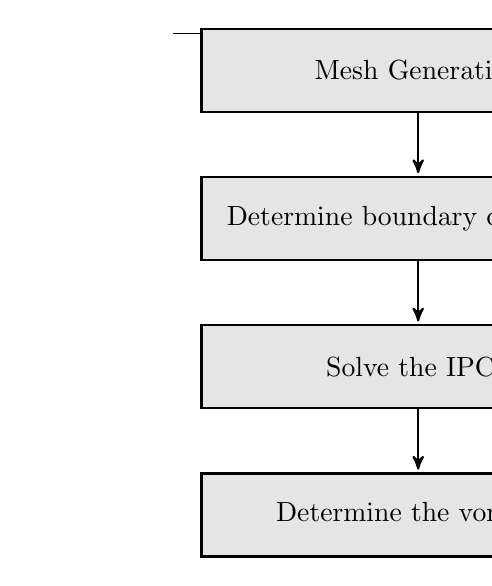
\begin{tikzpicture}
			[node distance=.8cm, start chain=going below,]
			\node[punktchain, join] (meshGen) {Mesh Generation};
		    \node[punktchain, join] (bc) {Determine boundary conditions};
		    \node[punktchain, join] (solve)     {Solve the IPCS};
		    \node[punktchain, join] (vort) 	  {Determine the vorticity};
		\end{tikzpicture}
		\caption{Flowchart of the Eulerian method.}
		\label{fig:flowchart_eulerian}
	\end{figure}	
	
The flowchart of the Eulerian method is given by Figure \ref{fig:flowchart_eulerian}.The algorithm to the Eulerian method can be summarized as follows:
	\begin{enumerate}
	\item \textbf{Mesh generation}: We generate the mesh of the fluid domain using \gmsh before the iteration.
	\item \textbf{Determine the boundary condition}: We determine the boundary conditions for the boundary domains: $\partial \Omega_E = \Sigma_{w} \cup \Sigma_{d} \cup \Sigma_{p}$. If we have Dirichlet velocity boundary conditions for all the exterior boundaries, we do not have to apply any pressure boundary conditions at $\partial \Sigma_{p}$, because $\Sigma_{p}=\emptyset$ in that case.
	\item \textbf{Solve the IPCS}: Using IPCS, time march from $t_n$ to $t_{n+1}$ to solve for the new velocity $\mathbf{u}$ and pressure $p$ field.
	\item \textbf{Determine the vorticity}: Using the algorithm described in \ref{subsec:dtvf}, solve for the vorticity field $\omega$ at the time $t_{n+1}$. 
	\end{enumerate}
	
Once we have the well-resolved vorticity $\omega$ of the near-body region, the vorticity is then transfered into the Lagrangian subdomain using the Hybrid coupling scheme, which was summarized in the introduction, chapter \ref{ch:introduction}, and fully elaborated in chapter \ref{ch:hybrid}.

\section{Validation of Eulerian Method}
\label{sec:eu-voem}

To verify our Eulerian method, we first investigated the Lamb-Oseen vortex problem. The validation of the Eulerian method is done by investigating the Clercx-Bruneau dipole collision at $Re=625$, comparing with the study of Clercx and Bruneau \cite{Clercx2006a}. Furthermore, we investigated the problem of the impulsively started cylinder at $Re=550$, where we verified and validated the lift and drag calculations with the literature of Koumoutsakos and Leonard \cite{Koumoutsakos1995a}, and Rosenfeld et al. \cite{MosheRosenFeldDochanKwak1991}.

\subsection{Lamb-Oseen Vortex}
\label{subsec:eulerianLambOseen}

The Lamb-Oseen vortex is an analytical solution by Lamb and Oseen, describing the diffusion of a vortex core \cite{Tryggeson2007}. The current investigation was performed similarly to the Lagrangian study in section \ref{subsec:lagrangianLambOseen}. 
%We solved the same problem as the one described in the Lagrangian validation problem \ref{subsec:lagrangianLambOseen}. 

\subsubsection*{Problem Definition}

%In the Lagrangian method, the Lamb-Oseen vortex was initialized using the vorticity field as the vortex blobs carry circulation strengths. However, Eulerian domain use the primitive variables $\mathbf{u}-p$ for formulating the problem. Therefore, we use the Lamb-Oseen velocity field as the initial conditions for the problem. 
%	\ctable[
%		caption = {Summary of the parameters for the Lamb-Oseen vortex evolution.},
%		label   = {tab:eulerianLambOseenParams},
%		pos = !b,]{lcll}{}{\FL
%		
%		Parameters 					& Value 	& Unit					& Description \ML
%		$\Gamma_c$\T               	& 1 &\si{m^2.s^{-1}} 				& Core strength\\
%		$\Omega$               		& $\left[-1,1\right]\times \left[-1,1\right]$ &\si{m}		& Eulerian domain bounds \\
%		$\mathbf{u}_{\infty}$ 		& $0$ &\si{m.s^{-1}} & Free-stream velocity\\
%		$\nu$						& $\num{5e-4}$ &\si{kg.s^{-1}.m^{-1}}& Kinematic viscosity\\
%			$ \tau$ 		    & 4 &\si{s}	& Lamb-Oseen time constant\\
%		$ t$ 		    	& \numrange{0}{1} &\si{s}			& Simulation time span\\		
%		$ \Delta t$ 				& $0.001$ &\si{s}					& Time step size\\
%		$ N_{\mathrm{t-steps}}$ 	& 1000 & -							& Number of time integration steps\\		
%		$ h_{\mathrm{min}}$			& $\frac{1}{100}\sqrt{2}$ &\si{m}	& Minimum mesh cell size\\	        
%		$ N_{\mathrm{cells}}$ 		& $200^2$ 	& -						& Number of mesh cells\\
%		$ \mathrm{CFL}$								& $0.95$ & -		& CFL number\\	        	        
%		$\lVert \mathbf{u} \rVert_{\mathrm{max}}$	& $1.5$	& 	\si{m.s^{-1}} & Maximum magnitude fo the velocity\\	
%		Time integration & FE & - & Forward Euler time integration method\LL}

	\ctable[
		caption = {Summary of the parameters for the Lamb-Oseen vortex evolution.},
		label   = {tab:eulerianLambOseenParams},
		pos = !b,]{lcll}{}{\FL
		
		Parameters 					& Value 	   & Description \ML
		$\Gamma_c$\T               	& 1 			& Core strength\\
		$\Omega$               		& $\left[-1,1\right]\times \left[-1,1\right]$ 	& Eulerian domain bounds \\
		$\mathbf{u}_{\infty}$ 		& $0$ & Free-stream velocity\\
		$\nu$						& $\num{5e-4}$ & Kinematic viscosity\\
			$ \tau$ 		    & 4 & Lamb-Oseen time offset\\
		$ t$ 		    	& \numrange{0}{1} 			& Simulation time span\\		
		$ \Delta t$ 				& $0.001$ 				& Time step size\\
		$ N_{t}$ 	& 1000 					& Number of time integration steps\\		
		$ h_{grid}$			& $\approxeq0.01$   & Minimum mesh cell size\\	        
		$ N_{cells}$ 		& $161312$ 					& Number of mesh cells\\
		$ \mathrm{CFL}$								& $0.95$ 	& CFL number\\	        	        
		$\lVert \mathbf{u} \rVert_{\mathrm{max}}$	& $1.5$	& 	Maximum magnitude of the velocity\\	
		Time integration & FE & Forward Euler time integration method\LL}

In section \ref{subsec:lagrangianLambOseen}, the vortex blobs of the Lagrangian method required the vorticity formulation of the Lamb-Oseen vortex to set up the problem. However, as the Eulerian method use the primitive variables $\mathbf{u}-p$, we require the velocity formulation of the Lamb-Oseen vortex. The velocity field of the Lamb-Oseen vortex is defined as,
	\begin{subequations}
	\begin{align}
	u_{\theta} &= \frac{\Gamma_c}{2\pi r} \left[1-\exp\left(-\frac{r^2}{4\pi\nu(t+\tau)}\right)\right]\\
	u_r &= 0,
	\end{align}
	\label{eq:eLO_veq}
	\end{subequations}	
where $u_{\theta}$ is the circumferential velocity, and $u_r$ is the radial velocity. The velocity is a function of the vortex core strength $\Gamma_c$, the simulation time $t\in[0,\infty[$, the time constant $\tau$, the kinematic viscosity $\nu$, and the distance from the core center $r$.

The parameters used for the simulation are tabulated in table \ref{tab:eulerianLambOseenParams}. To ensure a valid comparison of the present Eulerian method study with the Lagrangian method performed in section \ref{subsec:lagrangianLambOseen}, we chose similar spatial discretization parameters.

	\begin{figure}[!t]
	\centering
	\includegraphics[width=0.5\linewidth]{./figures/eulerian/lambOseenDomainDefinition-crop.pdf}
	\caption{Eulerian domain $\Omega_E$ ({\color{plotGray}{\textbf{gray}}}) for the Lamb-Oseen vortex problem, bounded by the Dirichlet velocity boundary $\Sigma_d$ ({\color{plotRed}{\textbf{red}}}), where the Dirichlet velocity boundary condition was applied. The parameters of the domain are tabulated in table \ref{tab:eulerianLambOseenParams}.}
	\label{fig:lambOseenDomainDefinition}
	\end{figure}

Figure \ref{fig:lambOseenDomainDefinition} depicts the domain for the present Lamb-Oseen vortex study. The fluid domain $\Omega_E$ is bounded by a Dirichlet boundary $\Sigma_d$ such that $\partial \Omega_E = Sigma_d$. The Dirichlet boundary $\Sigma_d$ is used to prescribe the analytical Dirichlet velocity boundary conditions for the Lamb-Oseen vortex problem.
 
The Eulerian method is time marched using the time integration parameters tabulated in table \ref{tab:eulerianLambOseenParams}. To ensure a stable time integration, we enforced the CFL conditions, equation \ref{eq:cfl}. During the evolution of the solution, we evaluated the growth of the error in velocity, and the error in vorticity between the numerical and the analytical solutions.

%where $\Gamma_c$ is the vortex core strength, $\tau \equiv \nu t$ is the scaled viscous time, and $r$ is the distance from the core center. The parameters of the simulation is tabulated in table \ref{tab:eulerianLambOseenParams}. To ease the comparison of the Eulerian to the Lagrangian method, we performed ensure similar spatial resolution. The figure \ref{fig:lambOseenDomainDefinition} shows the domain of the problem, discretized the domain $\Omega = \left[-1,1\right]^2$ in a structure grid with the number of finite element cells $N_{\mathrm{cells}}=200^2$ in $x$ and $y$ direction, minimum cell size $h=\sqrt{2}/100$. 



%Furthermore, the figure \ref{fig:lambOseenDomainDefinition} also shows the boundary domains $\partial \Omega$ of the fluid domain. For the Lamb-Oseen problem, as we have the analytical solution of the velocity field for all time, we can use this solution to prescribe the external domain boundary condition. So for this problem, we only need an external Dirichlet velocity boundary condition, at the boundary domain identified as, $\mathrm{ID}_{\mathrm{ext}} = 3$. This would imply that we do not need to explicitly apply the pressure boundary condition, as we already have a velocity boundary condition. With all the boundary conditions, we can evolve the initial velocity distribution of the Lamb-Oseen vortex from $t_0 = 4$ to $t_f =5$, using the IPCS algorithm described in section \ref{subsec:ipcs}. 

%	\begin{figure}[p]
%	\centering
%	\includegraphics[width=0.99\linewidth]{./figures/eulerian/lambOseen_eulerian_wRelField_compressed.pdf}
%	\caption{Relative error in vorticity field in logarithmic scale. Figure \textbf{(a)} shows the initial relative error in vorticity at $t=0$, and figure \textbf{(b)} shows the relative error in vorticity at the end of the time stepping $t=1$. The parameters of the simulation are tabulated in table \ref{tab:eulerianLambOseenParams}.}
%	\label{fig:lambOseen_eulerian_wRelField_compressed}
%	\end{figure}
	
	\begin{figure}[p]
     \centering
     \begin{subfigure}[b]{0.45\textwidth}
             \includegraphics[width=\textwidth]{figures/eulerian/lambOseen_wErrorInitial_compressed-crop.png}
             \caption{$t=0$}
             \label{fig:lambOseen_wErrorInitial_compressed-crop}
     \end{subfigure}%
     \qquad %add desired spacing between images, e. g. ~, \quad, \qquad etc.
       %(or a blank line to force the subfigure onto a new line)
     \begin{subfigure}[b]{0.45\textwidth}
             \includegraphics[width=\textwidth]{figures/eulerian/lambOseen_wErrorFinal_compressed-crop.png}
             \caption{$t=1$}
             \label{fig:lambOseen_wErrorFinal_compressed-crop}
     \end{subfigure}
     
     \caption{Relative error in vorticity (in logarithmic scale) using the parameters tabulated in table \ref{tab:eulerianLambOseenParams}. The figure shows \textbf{(a)}, the initial relative error in vorticity at $t=0$, and \textbf{(b)} the final relative error in vorticity at $t=1$.}
     \label{fig:lambOseen_eulerian_wRelField_compressed}
	\end{figure}	
	
	\begin{figure}[p]
	\centering
	\includegraphics[width=0.6\linewidth]{./figures/eulerian/lambOseen_eulerian_wRelEvolution_compressed.pdf}
	\caption{Evolution of the maximum relative errors from $t=0$ to $t=1$ using the parameters in table \ref{tab:eulerianLambOseenParams}. The figure depicts maximum relative error in velocity [{\color{plotBlue}{---}}, solid {\color{plotBlue}{\textbf{blue}}}] and the maximum relative error in vorticity [---, solid \textbf{black}]. }
	\label{fig:lambOseen_eulerian_wRelEvolution}
	\end{figure}


	\begin{figure}[p]
        \centering
        \begin{subfigure}[b]{0.5\textwidth}
                \includegraphics[width=\textwidth]{figures/eulerian/lambOseen_eulerianConvergence_dx_compressed.pdf}
                \caption{Spatial convergence}
                \label{fig:lambOseen_eulerianConvergence_dx}
        \end{subfigure}%
        ~ %add desired spacing between images, e. g. ~, \quad, \qquad etc.
          %(or a blank line to force the subfigure onto a new line)
        \begin{subfigure}[b]{0.5\textwidth}
                \includegraphics[width=\textwidth]{figures/eulerian/lambOseen_eulerianConvergence_dt_compressed.pdf}
                \caption{Temporal convergence}
                \label{fig:lambOseen_eulerianConvergence_dt}
        \end{subfigure}
        \caption{Convergence in space and time. The figure depicts \textbf{(a)} convergence in space of $\mathcal{O}(\Delta h^2)$ and \textbf{(b)} convergence in time of $\mathcal{O}(\Delta t)$. The control parameters are tabulated in table \ref{tab:eulerianLambOseenParams}.}
        \label{fig:lambOseen_eulerianConvergence}
	\end{figure}		
	

%We used $CFL$ stability condition equation \ref{eq:cfl}, to determine the time step size, $\Delta t = 0.001$. The Eulerian method time steps using a \printAcron{Forward Euler}{FE} time marching and requires $N_{\mathrm{t-steps}}=1000$ time steps. During the evolution, we evaluated the growth of the error in velocity, and in vorticity between the numerical results and the analytical solution. 

\subsubsection*{Results and Discussion}

We are interested in the evolution of error in vorticity, as this is the quantity which will be interpolated onto the Lagrangian subdomain. Figure \ref{fig:lambOseen_eulerian_wRelField_compressed} shows the initial and the final relative error in vorticity over the Eulerian domain. Opposed to the Lagrangian results, Figure \ref{fig:lambOseen_convection_vorticityErrorContours}, we see that initial relative error in the vorticity field is larger. This is so because the Eulerian solution was initialized using the velocity and the vorticity is obtained by projecting $\nabla\times\mathbf{u}$ (see section \ref{subsec:dtvf}
) onto the scalar-valued function space $W$, whereas the Lagrangian solution was initialized directly from vorticity. This process of initialization in the Eulerian domain introduces additional numerical error in the vorticity. However, the pattern of the relative error in vorticity is similar to the Lagrangian solution, with the highest error at the core center, where we have stronger vorticity.

As time progresses, we see that the error in the solution does not increase as observed for the Lagrangian method, Figure \ref{fig:lambOseen_eulerian_wRelField_compressed}b. Figure \ref{fig:lambOseen_eulerian_wRelEvolution} shows this change in the maximum relative error in velocity and vorticity. The maximum relative error in vorticity is at all times higher than the maximum relative error in velocity, due to the error in projection.

To determine the convergence with spatial resolution, the simulation was run for $h \approx 0.25$ to $h \approx \num{5e-3}$. Figure \ref{fig:lambOseen_eulerianConvergence_dx} shows the convergence of the relative error in vorticity. This validates that the scheme is $2^{\mathrm{nd}}$-order in space, which is expectable due to the second order function space $\mathrm{CG}_2$ for the primitive variable, velocity.

To determine convergence with time resolution, we ran the simulation with various time steps $\Delta t = \num{5e-3}$ to $\Delta t = \num{1e-4}$. As we performed the investigation, we saw that the error in the primitive variable $\mathbf{u}$, converged with order 1, Figure \ref{fig:lambOseen_eulerianConvergence}. This is expected, as have employed a $1^{\mathrm{st}}$-order Forward Euler scheme. Thus, we have verified against the analytical solution of the Lamb-Oseen vortex that our Eulerian method is well implemented and performs in a robust manner.

\subsection{Clercx-Bruneau Dipole Collision at $Re=625$}
\label{subsec:eul_cbdc}
The Eulerian method that we have developed here is to be used as a wall-bounded Eulerian solver that can resolve the vorticity production at the boundary for the Hybrid method. Therefore it is vital that the vortex interaction with the no-slip boundary is handled properly.

To determine the proper handling of the no-slip boundary, it is common practice to use a simple test of dipole colliding with the wall. In these test cases, one could observe how the no-slip boundary handles the incoming vortex and can be used to determine if the system is formulated appropriately.  Ould-Salihi et al. \cite{Ould-Salihi2001a} used this case to validate their Hybrid method that couples vortex particles with finite-difference method. Cottet et al. \cite{Cottet2000b} used this test case to validate the vortex method. Therefore in a similar fashion, we have decided to use the dipole collision study by Clercx and Bruneau \cite{Clercx2006a}, performed using a Chevyshev pseudo-spectral method, to verify and validate our Eulerian method. 

%Therefore, we decided to use the Clercx-Bruneau dipole collision is a test case from Clercx \& Bruneau \cite{Clercx2006a}, where they performed a numerical study of a normal collision of a dipole with a no-slip boundary. This experiment provide extensive benchmark results for various Reynolds numbers with a Chevyshev pseudo-spectral numerical method. 

\subsubsection*{Problem Definition}

Unlike other dipole test cases, Clercx and Bruneau provide well-defined initial and boundary conditions for the dipole vorticity field. Furthermore, they used a vorticity distribution that was continuous, which ensures a smooth velocity field for our Eulerian method using the $\mathbf{u}-p$ formulation. The literature provided results for the collision that we are interested: a normal collision with the dipole traveling perpendicular to the wall.

	\begin{figure}[!b]
     \centering
     \begin{subfigure}[t]{0.45\textwidth}
             \includegraphics[width=\textwidth]{figures/eulerian/clercxBruneauDomainDefinition-crop.pdf}
             \caption{(\textit{Not to scale}) Domain definition}
             \label{fig:clercxBruneauDomainDefinition}
     \end{subfigure}%
     \qquad %add desired spacing between images, e. g. ~, \quad, \qquad etc.
       %(or a blank line to force the subfigure onto a new line)
     \begin{subfigure}[t]{0.45\textwidth}
             \includegraphics[width=\textwidth]{figures/eulerian/clercxBruneauDomainMesh-crop.png}
             \caption{Domain mesh}
             \label{fig:clercxBruneauDomainMesh}
     \end{subfigure}
     \caption{Domain of the Clercx-Bruneau dipole collision problem. The figure depicts \textbf{(a)} the definition of the domain with the fluid domain ({\color{plotGray}{\textbf{gray}}}) and the no-slip boundary ({\color{plotBlue}{\textbf{blue}}}); and \textbf{(b)} the unstructured mesh of the domain with $N_{\mathrm{vert}} = 48k$.}
     \label{fig:clercxBruneauDomain}
	\end{figure}

For the present study, we have decided to use the simpler case of $Re=625$, where $Re$ is the integral-scale Reynolds number defined as,
	\begin{equation}
	Re = \frac{UW}{\nu},
	\end{equation}
where $U$ is the characteristic velocity of the flow, $W$ is half width of domain, and $\nu$ is the kinematic viscosity and are chosen according to Clercx and Bruneau \cite{Clercx2006a}. A low Reynolds number of $Re=625$ is required as the Eulerian method currently only solves an incompressible laminar flow. However in future, an implementation of a turbulence method can enable a high Reynolds number investigation.

The domain $\Omega$ of the problem is square, $\Omega_E = [-1,1]\times[-1,1]$, as shown in Figure \ref{fig:clercxBruneauDomainDefinition}. The problem is defined in a closed box, where the Eulerian domain is enclosed in a no-slip boundary $\partial{\Omega} = \Sigma_w$ where dipole collides and interacts.

The initial condition of the Clercx-Bruneau dipole is a smooth dipole velocity distribution with a positive monopole at $(x_1,y_1)=(0.1,0)$ and the negative monopole at $(x_2,y_2)=(-0.1,0)$, with each having a core radius $R = 0.1$. The velocity distribution for the combined monopole at $t=0$ is given as,
	\begin{subequations}
	\begin{align}
	u(\mathbf{x},0) & = -\frac{1}{2}\omega_e(y-y_1)\exp\left\{-\left(\frac{r_1}{R}\right)^2\right\} + \frac{1}{2}\omega_e(y-y_2)\exp\left\{-\left(\frac{r_2}{R}\right)^2\right\}, \\
	v(\mathbf{x},0) & = +\frac{1}{2}\omega_e(x-x_1)\exp\left\{-\left(\frac{r_1}{R}\right)^2\right\} - \frac{1}{2}\omega_e(x-x_2)\exp\left\{-\left(\frac{r_2}{R}\right)^2\right\},
	\end{align}
	\label{eq:clercxBruneauVel0}
	\end{subequations}
where $u$ and $v$ are the velocities in the $x$ and $y$ direction, respectively. The characteristic vorticity magnitude $\omega_e = 299.528385375226$ is obtained from Renac et. al \cite{Renac2013}. The radii $r_1$ and $r_2$ are the radial distances to the point $\mathbf{x}$ from the center of positive and the negative monopoles respectively. The corresponding vorticity distribution for the velocity distribution is given as,
	\begin{equation}
	\begin{split}
	\omega(\mathbf{x},0) = \quad &\omega_e\left[1-\left(\frac{r_1}{R}\right)^2\right]\exp\left\{-\left(\frac{r_1}{R}\right)^2\right\} \\
	-\ &\omega_e\left[1-\left(\frac{r_2}{R}\right)^2\right]\exp\left\{-\left(\frac{r_1}{R}\right)^2\right\}.
	\end{split}
	\label{eq:clercxBruneauOmega0}
	\end{equation}

The Eulerian domain was discretized using an unstructured meshing method in GMSH (section \ref{subsec:mgugmsh}), as shown in Figure \ref{fig:clercxBruneauDomainDefinition}. The velocity distribution, equation \ref{eq:clercxBruneauVel0}, shows that the maximum velocity in the fluid will be along the $y$-axis (i.e $x=0$). Therefore, to satisfy the $CFL$ condition, we need the minimum cell size at the location of the maximum velocity. The resolution of the mesh in the region where the dipole and the wall interacts (i.e $-0.5\le{x}\le0.5$ and $0.5\le{\left|y\right|}\le1$) was also increased. Furthermore, in the region where there is no vorticity, we do not need high resolution (i.e $0.5\le{\left|x\right|}\le1$ and $-0.5\le{y}\le0.5$). 

After initializing the velocity field in the discretized domain, the problem was evolved from $t=0$ to $t=2$. The time integration parameters are tabulated in table \ref{tab:clercxBruneauParameters}.

	\ctable[
		caption = {Summary of the parameters for the Clercx-Bruneau dipole collision with a no-slip wall \cite{Clercx2006a}.},
		label   = {tab:clercxBruneauParameters},
		pos = !t,]{lcll}{\tnote[a]{Obtained from Clercx and Bruneau \cite{Clercx2006a}}
						 \tnote[b]{Obtained from Renac et al. \cite{Renac2013}}}{\FL
		Parameters					& Value 				& Description \ML
		$\Omega$               		& $\left[-1,1\right]\times[-1,1]$ & Eulerian domain bounds \\
		$Re$  			       		& $625$ 				& Reynolds number \\ 
		$U$			         		& $1$\tmark[a]			& Characteristic velocity\\		
		$W$			         		& $1$\tmark[a]			& Half width of the domain\\		
		$\nu$						& $\num{1.6e-3}$ 		& Kinematic viscosity\\
		$ (x,y)_{1,2}$				& $(\pm0.1,0)$			& Initial location of the monopoles\\
		$ \omega_e$		            & $299.5283853752226$\tmark[b]  	&  Characteristic vorticity of the monopole\\
		$ t$ 		    	& 0 to 2				& Simulation time span\\
		$ \mathrm{CFL}$				& $0.95$ 				& CFL number\\	        	        
		$ \lVert\mathbf{u}\rVert_{\mathrm{max}}$	& $12$	& Maximum fluid velocity\\
		$ \Delta t$ 		    	& $\num{1.25e-5}$		& Time step size\\
		$ N_{cells}$ 		& 96142 			& Number of FE mesh cells\\
		$ h_{grid}$			&\num{3.6e-3} to \num{5.1e-2}	        & FE mesh cell size\\	        
		$ N_{t}$ 		& $160,000$	 	& Number of time integration steps\LL}

%	\ctable[
%		caption = {Summary of the parameters for the Clercx-Bruneau normal collision of a dipole with a no-slip wall \cite{Clercx2006a}.},
%		label   = {tab:clercxBruneauParameters},
%		pos = !t,]{lcll}{\tnote[a]{Obtained from Clercx and Bruneau \cite{Clercx2006a}}
%						 \tnote[b]{Obtained from Renac et al. \cite{Renac2013}}}{\FL
%		Parameters					& Value 				& Unit		& Description \ML
%		$\Omega$               		& $\left[-1,1\right]\times[-1,1]$ &\si{m}		& Eulerian domain bounds \\
%		$Re$  			       		& $625$ 				&-			& Reynolds number \\ 
%		$U$			         		& $1$\tmark[a]			&\si{m.s^{-1}}& Characteristic velocity\\		
%		$W$			         		& $1$\tmark[a]			&\si{m}		& Half width of the domain\\		
%		$\nu$						& $\num{1.6e-3}$ 		&\si{kg.s^{-1}.m^{-1}}& Kinematic viscosity\\
%		$ (x,y)_{1,2}$				& $(\pm0.1,0)$			& \si{m}    & Initial location of the dipole\\
%		$ \omega_e$		            & $299.5283853752226$\tmark[b] & -   	&  Characteristic vorticity of the monopole\\
%		$ t$ 		    	& 0 to 2				& - 	& Simulation time\\
%		$ \mathrm{CFL}$				& $0.95$ 				& -			& CFL number\\	        	        
%		$ \lVert\mathbf{u}\rVert_{\mathrm{max}}$	& $12$	& \si{m.s^{-1}}	& Maximum fluid velocity\\
%		$ \Delta t$ 		    	& $\num{1.25e-5}$		& \si{s} 	& Time step size\\
%		$ N_{\mathrm{vert}}$ 		& $\sim48k$ 			& -			& Number of mesh vertices\\
%		$ h_{\mathrm{min}}$			& $\sim\num{3.6e-3}$ &\si{m}		& Minimum mesh cell size\\	        
%		$ N_{\mathrm{tsteps}}$ 		& $160,000$				& -	     	& Number of time integration steps\\
%		$\mathrm{ID}_{\mathrm{fluid}}$ & $1$ 				& - 		& Fluid domain I.D\\
%		$\mathrm{ID}_{\mathrm{wall}}$ & $2$ 				& - 		& No-slip boundary I.D\LL}

%The initial condition of the Clercx-Bruneau dipole is a smooth dipole vorticity distribution with a positive monopole at $(x_1,y_1)=(0.1,0)$ and the negative monopole at $(x_2,y_2)=(-0.1,0)$, with each having a core radius $R = 0.1$. The vorticity distribution of the combined monopole is given as,
%	\begin{equation}
%	\begin{split}
%	\omega(\mathbf{x},0) = \quad &\omega_e\left[1-\left(\frac{r_1}{R}\right)^2\right]\exp\left\{-\left(\frac{r_1}{R}\right)^2\right\} \\
%	-\ &\omega_e\left[1-\left(\frac{r_2}{R}\right)^2\right]\exp\left\{-\left(\frac{r_1}{R}\right)^2\right\} ,
%	\end{split}
%	\label{eq:clercxBruneauOmega0}
%	\end{equation}
%where $\omega_e = 299.528385375226$, obtained from Renac et. al \cite{Renac2013}. The radii $r_1$ and $r_2$ are the radial distances to the point $\mathbf{x}$ from the center of positive and the negative monopoles respectively. Figure \ref{fig:dipole_contourLine_portrait}a shows the vorticity contours of this initial vorticity distribution. The initial vorticity distribution decays at an exponential rate to zero at the no-slip boundary. This means the no-slip boundary condition is still guaranteed for the initial distribution. To initialize the problem in the Eulerian domain with $\mathbf{u}-p$, we used the velocity distribution, 
%	\begin{subequations}
%	\begin{align}
%	u(\mathbf{x},t) & = -\frac{1}{2}\lvert\hat{\omega}_1\rvert(y-y_1)\exp\left\{-\left(\frac{r_1}{R}\right)^2\right\} + \frac{1}{2}\lvert\hat{\omega}_2\rvert(y-y_2)\exp\left\{-\left(\frac{r_2}{R}\right)^2\right\}, \\
%	v(\mathbf{x},t) & = +\frac{1}{2}\lvert\hat{\omega}_1\rvert(x-x_1)\exp\left\{-\left(\frac{r_1}{R}\right)^2\right\} - \frac{1}{2}\lvert\hat{\omega}_2\rvert(x-x_2)\exp\left\{-\left(\frac{r_2}{R}\right)^2\right\},
%	\end{align}
%	\label{eq:clercxBruneauVel0}
%	\end{subequations}
%where $u$ and $v$ are the velocity in the $x$ and $y$ direction, respectively. The fluid domain of the Eulerian domain, show in figure \ref{fig:clercxBruneauDomainDefinition} was discretized using an controlled unstructured meshing method. From the velocity distribution, equation \ref{eq:clercxBruneauVel0}, we see that the maximum velocity in the fluid will be along the $y$-axis (i.e $x=0$). Therefore, to satisfy the $CFL$ condition, we need the minimum cell size at the location of the maximum velocity. Furthermore, to ensure the vorticity generation at the no-slip boundary is defined accurately, we increased resolution of the mesh at the boundary. The third region where we increased the resolution is where the dipole and the wall interacts (i.e $-0.5\le{x}\le0.5$ and $0.5\le{\left|y\right|}\le1$). In the region where there is no vorticity, we do not need high resolution (i.e $0.5\le{\left|x\right|}\le1$ and $-0.5\le{y}\le0.5$). With these parameterization, we obtained an unstructured grid with $N_{\mathrm{vert}}=48k$ vertices.

\subsubsection*{Results and Discussion}

Figure \ref{fig:dipole_contourLine_portrait} shows the evolution of the vorticity field at various instances, $t = [0, 0.25, 0.5,$ $0.75, 1.25]$. During the initial stages of the simulation, the initialized dipole travels along the $y$-axis towards the bottom no-slip boundary. 

	\begin{figure}[!p]
	\centering
	\includegraphics[width=\linewidth]{./figures/eulerian/dipole_contourLine_portrait-crop.pdf}
	\caption{Vorticity contour plots of the Clercx-Bruneau dipole-wall collision at $Re=625$ and $t = [0, 0.25, 0.5, 0.75, 1.0, 1.25]$ with vorticity contour levels at $[-320,-200,-100,$ $-50,-10,10, 50, 100, 200, 320]$. The figure depicts positive contours [---, solid \textbf{black}], and negative contours [- -, dashed \textbf{black}].}
	\label{fig:dipole_contourLine_portrait}
	\end{figure}

The dipole approaches the bottom boundary, where the no-slip boundary generates vorticity to ensure no-through flow, seen in Figure \ref{fig:dipole_contourLine_portrait}{\color{darkblue}{b}}. As the dipole approaches the wall, the vorticity filament at the wall rolls up and combines with the primary dipole forming two secondary dipoles, that is symmetric across the $y$-axis. Figure \ref{fig:dipole_contourLine_portrait}{\color{darkblue}{c}} shows the state of the vorticity field at $t=0.5$ after the secondary dipoles are generated. This secondary dipole initially travels away from the bottom wall and later on approaches the wall again, colliding for a second time and creating a tertiary vortex, Figure \ref{fig:dipole_contourLine_portrait}{\color{darkblue}{d}}. The dipole stops convecting any further and diffuses as time progresses, as shown in Figure \ref{fig:dipole_contourLine_portrait}{\color{darkblue}{e}} and \ref{fig:dipole_contourLine_portrait}{\color{darkblue}{f}}, corresponding to $t = 1$ and $t = 1.25$.

Figure \ref{fig:vorticity_contour_comparison} compares the vorticity contours of the computational domain close to the bottom wall, $0\leqslant x \leqslant 0.6$ and $-1 \leqslant y \leqslant -0.4$, at $t = 1$. The positive vortex (solid black) is surrounded by the negative vortex (dashed black). Comparing the present study, Figure \ref{fig:dipole_contourLine_t1p0} with the study of Clercx and Bruneau \cite{Clercx2006a}, Figure \ref{fig:VorticityContourPlot}, shows that the shows that the shape of the vorticity contours is indistinguishable. This means that the present study matches very well with the pseudo-spectral simulation of the Clercx and Bruneau.

	\begin{figure}[!t]
     \centering
     \begin{subfigure}[t]{0.4\textwidth}
             \includegraphics[width=\textwidth]{figures/eulerian/VorticityContourPlot-rotated270.pdf}
             \caption{Literature}
             \label{fig:VorticityContourPlot}
     \end{subfigure}%
     ~ %add desired spacing between images, e. g. ~, \quad, \qquad etc.
       %(or a blank line to force the subfigure onto a new line)
     \begin{subfigure}[t]{0.45\textwidth}
             \includegraphics[width=\textwidth]{figures/eulerian/dipole_contourLine_t1p0_corrected-crop.pdf}
             \caption{Present study}
             \label{fig:dipole_contourLine_t1p0}
     \end{subfigure}
     \caption{Comparison of the vorticity contours at $t=1$ with contour levels $[...,-50,$ $-30,-10,10,30,50,...]$. The figure compares the plot obtained by \textbf{(a)} literature of Clercx and Bruneau \cite{Clercx2006a} and \textbf{(b)} the present study.}
     \label{fig:vorticity_contour_comparison}
	\end{figure}
	
	\begin{figure}[!p]
     \centering
     \begin{subfigure}[t]{0.49\textwidth}
             \includegraphics[width=\textwidth]{figures/eulerian/dipole_KineticEnergy_comparison.pdf}
             \caption{Kinetic Energy $E(t)$}
             \label{fig:dipole_KineticEnergy_comparison}
     \end{subfigure}%
     ~ %add desired spacing between images, e. g. ~, \quad, \qquad etc.
       %(or a blank line to force the subfigure onto a new line)
     \begin{subfigure}[t]{0.49\textwidth}
             \includegraphics[width=\textwidth]{figures/eulerian/dipole_Enstrophy_comparison.pdf}
             \caption{Enstrophy $\Omega(t)$}
             \label{fig:dipole_Enstrophy_comparison}
     \end{subfigure}
     
     \begin{subfigure}[b]{0.49\textwidth}
             \includegraphics[width=\textwidth]{figures/eulerian/dipole_Palinstrophy_comparison.pdf}
             \caption{Palinstrophy $P(t)$}
             \label{fig:dipole_Palinstrophy_comparison}
     \end{subfigure}
    
     \caption{Comparison of the fluid parameters from $t=0$ to $t=2$ with reference data obtained from Clercx and Bruneau \cite{Clercx2006a} [{\color{plotRed}{$\bullet$}}, {\color{plotRed}{\textbf{red}}} dot]. The figure shows the evolution of \textbf{(a)} the kinetic energy $E(t)$, \textbf{(b)} the enstrophy $\Omega(t)$, and \textbf{(c)} the palinstrophy $P(t)$.}
     \label{fig:dipole_comparison}
	\end{figure}
		
	\begin{figure}[!p]
	\centering
		\includegraphics[width=0.6\textwidth]{./figures/eulerian/VorticityAtBoundary2.pdf}
		\caption{The vorticity generated at the bottom-left wall ($y=-1$, $-0.6\leqslant x \leqslant 0$) at $t=0.4$ [{\color{plotBlue}{---}}, solid blue], $t=0.6$ [{\color{plotRed}{---}}, solid red] and $t=1$ [{\color{plotGreen}{---}}, solid green]. The results are compared with Clercx and Bruneau \cite{Clercx2006a} (dotted).}
		\label{fig:VorticityAtBoundary}
	\end{figure}	
	
To determine the variation of the fluid properties as time progresses, Clercx and Bruneau investigated the evolution of the total kinetic energy $E$, the total enstrophy $\Omega$, and the total palinstrophy $P$ of the flow field. The total kinetic energy $E$ of the flow can be determined with,
	\begin{equation}
	E(t) = \frac{1}{2} \int\int \mathbf{u}^2(\mathbf{x},t)\ \mathrm{d}x\mathrm{d}y,
	\end{equation}
and at $t=0$, we have $E(0) = 2$. The total enstrophy of the flow is determined as, 
	\begin{equation}
	\Omega(t) = \frac{1}{2}\int\int\omega^2(\mathbf{x},t)\ \mathrm{d}x\mathrm{d}y.
	\end{equation}	
The change in enstrophy of the flow field can give an insight into the dissipation rate in the fluid. At $t=0$, the total enstrophy of the fluid is $\Omega(0)=800$. The total palinstrophy $P$ of the flow measures the gradient of vorticity and is given by, 
	\begin{equation}
	P(t) = \frac{1}{2}\int\int\left[\nabla\omega(\mathbf{x},t)\right]^2\ \mathrm{d}x\mathrm{d}y,
	\end{equation}
and gives an insight into the generation of vorticity at the no-slip boundary. Figure \ref{fig:dipole_comparison} compares the evolution of these time dependent parameters with the reference data provided by Clercx and Bruneau. Clercx and Bruneau \cite{Clercx2006a} provide the values of the parameters at $t=0.25$, $t=0.5$ and $t=0.75$. 

Figure \ref{fig:dipole_KineticEnergy_comparison} shows the evolution of the kinetic energy. The kinetic energy $E$ reduced from $E(0) = 2$ to $E(2) \approx 0.3$. At $t=0.4$, we have small kink representing the approach of the primary dipole at the wall. When plotting the reference data, we see that the variation in kinetic energy matches perfectly at $t=0.25$, $t=0.5$ and $t=0.75$.

%	\ctable[
%	    caption = {A summary of the values of the first two maxima of the enstrophy $E$ and palinstrophy $P$ occurring at $t_1$ and $t_2$ respectively.},
%	    label   = {tab:euleriandipoleCollisionComparison},
%	    maxwidth = \textwidth,
%	    pos = !t,
%	]{ccrrrr}{\tnote{Data obtained from Clercx \& Bruneau \cite{Clercx2006a}}}{\FL
%	\multirow{2}{*}{Instant} & 	\multirow{2}{*}{Case} & \multicolumn{2}{c}{Enstrophy $\Omega$} & \multicolumn{2}{c}{Palinstrophy $P$}\\
%	\noalign{\smallskip}\cline{3-6}\noalign{\smallskip}
%			& 			& $t$ & $\Omega$ 	& $t$ & $P$\ML
%	\multirow{2}{*}{$1^{\mathrm{st}} peak$} 	& Reference\tmark[a] 	& 0.371 & 933.6 	& 0.361 & $1.39\times10^7$\\
%							& Present 		& 0.370 & 938.6 	& 0.360 & $1.40\times10^7$\\
%	\multirow{2}{*}{$2^{\mathrm{nd}} peak$} 	& Reference\tmark[a] 	& 0.648 & 305.2 	& 0.652 & $6.78\times10^{5}$\\
%							& Present 		& 0.650 & 307.0		& 0.650 & $6.90\times10^{5}$\LL}

%	\ctable[
%	    caption = {A summary of the values of the first two maxima of the enstrophy $E$ and palinstrophy $P$ occurring at $t_1$ and $t_2$ respectively.},
%	    label   = {tab:euleriandipoleCollisionComparison},
%	    maxwidth = \textwidth,
%	    pos = !t,
%	]{ccrr}{\tnote{Data obtained from Clercx \& Bruneau \cite{Clercx2006a}}}{\FL
%	\multirow{2}{*}{Instant} & 	\multirow{2}{*}{Case} & \multicolumn{2}{c}{$t$}\\
%	\noalign{\smallskip}\cline{3-4}\noalign{\smallskip}
%			& 			& Enstrophy $\Omega$ & Palinstrophy $P$ \ML
%	\multirow{2}{*}{$1^{\mathrm{st}}$ peak} 	& Reference\tmark[a] 	& 0.371 & 0.361 \\
%							& Present 		& 0.370 & 0.360 \\ \\ 
%	\multirow{2}{*}{$2^{\mathrm{nd}}$ peak} 	& Reference\tmark[a] 	& 0.648 & 0.652 \\
%							& Present 		& 0.650 & 0.650 \LL}


Figure \ref{fig:dipole_Enstrophy_comparison} shows the evolution of enstrophy $\Omega$ in time. During the initial instants, enstrophy decreases linearly and at $t=0.370$, there is sharp increase in the total enstrophy of the flow $\Omega(0.370) = 938.58$ (shown in blue). This indicates the initial impact of dipole with the no-slip wall. However, in literature \cite{Clercx2006a}, the initial peak occurs at $t=0.371$ with a peak enstrophy of $\Omega(0.371)=938.6$. Comparing these parameters we see that the enstrophy we calculate peaks earlier and with a larger values, meaning that our collision is slight early. However, the error in time of peaking is $0.3\%$ with a $0.6\%$ error in enstrophy, which is a significantly small error. We observe similar behaviour in the second collision, where the peak is our study is $\Omega(0.650)=307.04$ (shown in blue), whereas in literature the peak is $\Omega(0.648) = 305.2$. Again the error is relatively small implying that our Eulerian method resolves the evolution of enstrophy very well.

%After the impact, the enstrophy quickly drops and peaks again at $t=0.65$ reaching $\Omega(0.65) = 307.04$. Table \ref{tab:euleriandipoleCollisionComparison} shows the occurrence of the peak enstrophy for Clercx and Bruneau ??. We see that in the study of Clercx and Bruneau, the first peak occurred at $t=0.371$ and the second peak occured at $t=0.648$. This means a $0.3\%$ and a $0.6\%$ error in time for occurrence of the peak in enstrophy. The 

% implying that our Eulerian method resolves the evolution of enstrophy very well.

%In addition, to the 3 data points, Clercx \& Bruneau determined the peak enstrophy of flow. Table \ref{tab:euleriandipoleCollisionComparison} compares the difference between the present study and literature and we see that there is maximum of $0.3\%$ error in time $t$ and $0.6\%$ error in enstrophy $\Omega$. Therefore, the variation in enstrophy is well represented by our Eulerian method.

Figure \ref{fig:dipole_Palinstrophy_comparison} shows the evolution of palinstrophy $P$ in time. When the dipole collides, vorticity is generated from the wall to ensure no-through boundary condition, which results in a sharp increase in the gradient of the vorticity.  Similar to the evolution of enstrophy, we can observe to peaking at $t=0.360$ and $t=0.650$, with peak palinstrophy of $P(0.360)=1.40\times10^7$ and $P(0.650)=6.90\times10^{5}$, respectively (shown in blue). In literature however, the peak palinstrophy occurs at $P(0.361) =1.39\times10^7$ and 
$P(0.652)=6.78\times10^{5}$. This is an acceptable error and tells us the generation of vorticity in Eulerian method performs according to theory.

%Table \ref{tab:euleriandipoleCollisionComparison} compares the difference with the addition data provided and we see that there is a maximum error of $0.3\%$ in time $t$ and $1.8\%$ in palinstrophy $P$. This is an acceptable error and tells us the generation of vorticity in Eulerian method performs according to theory.
	
Figure \ref{fig:VorticityAtBoundary} compares the vorticity along the boundary of the domain at $y=-1$ for $-0.6 \leqslant x \leqslant 0$. The solid lines represent the present data, and is compared with the dotted data obtained from Clercx and Bruneau \cite{Clercx2006a}. The comparison is done for various time instances $t=0.4$, $t=0.6$ and $t=1.0$ and we can finally validate that the Eulerian method accurately represents vorticity generation from the wall.


%	\begin{figure}[p]
%     \centering
%     \begin{subfigure}[t]{0.49\textwidth}
%             \includegraphics[width=\textwidth]{figures/eulerian/dipole_KineticEnergy_comparison.pdf}
%             \caption{Kinetic Energy $E(t)$}
%             \label{fig:dipole_KineticEnergy_comparison}
%     \end{subfigure}%
%     ~ %add desired spacing between images, e. g. ~, \quad, \qquad etc.
%       %(or a blank line to force the subfigure onto a new line)
%     \begin{subfigure}[t]{0.49\textwidth}
%             \includegraphics[width=\textwidth]{figures/eulerian/dipole_Enstrophy_comparison.pdf}
%             \caption{Enstrophy $\Omega(t)$}
%             \label{fig:dipole_Enstrophy_comparison}
%     \end{subfigure}
%     
%     \begin{subfigure}[b]{0.49\textwidth}
%             \includegraphics[width=\textwidth]{figures/eulerian/dipole_Palinstrophy_comparison.pdf}
%             \caption{Palinstrophy $P(t)$}
%             \label{fig:dipole_Palinstrophy_comparison}
%     \end{subfigure}
%     ~
%     \begin{subfigure}[b]{0.48\textwidth}
%		\includegraphics[width=\textwidth]{./figures/eulerian/VorticityAtBoundary.pdf}
%		\caption{Vorticity at the boundary y = -1.}
%		\label{fig:VorticityAtBoundary}
%     \end{subfigure}     
%     
%     \caption{Comparison of the fluid parameters. Figure \textbf{(a)}, \textbf{(b)}, \textbf{(c)} compares the evolution of the fluid properties from $t=0$ to $t=2$. Figure \textbf{(d)} compares the vorticity generated at the bottom-left wall ($y=-1$, $-0.6\leqslant x \leqslant 0$) at $t=0.4$ [{\color{plotBlue}{---}}, solid blue], $t=0.6$ [{\color{plotRed}{---}}, solid red] and $t=1$ [{\color{plotGreen}{---}}, solid green].}
%     \label{fig:dipole_comparison}
%	\end{figure}

\subsection{Impulsively started cylinder at $Re=550$}
\label{subsec:eul_isc}
Finally, we an impulsively started cylinder at $Re=550$. This validation test ensured that we are able to determine correct forces acting on the body. 

\subsubsection*{Problem Definition}

	\begin{figure}[!p]
     \centering
     \begin{subfigure}[t]{0.45\textwidth}
             \includegraphics[width=\textwidth]{figures/eulerian/ISCDomainDefinition-crop.pdf}
             \caption{(\textit{Not to scale}) Domain definition}
             \label{fig:ISCDomainDefinition-crop}
     \end{subfigure}%
     ~ %add desired spacing between images, e. g. ~, \quad, \qquad etc.
       %(or a blank line to force the subfigure onto a new line)
     \begin{subfigure}[t]{0.45\textwidth}
             \includegraphics[width=\textwidth]{figures/eulerian/ISC_mesh-crop.png}
             \caption{Full mesh}
             \label{fig:ISC_mesh}
     \end{subfigure}

     \begin{subfigure}[t]{0.3\textwidth}
             \includegraphics[width=\textwidth]{figures/eulerian/ISC_mesh_surface-crop.png}
             \caption{Mesh near the surface}
             \label{fig:ISC_mesh_surface}
     \end{subfigure}

     \caption{Domain of the ISC problem. The figure depicts \textbf{(a)} the definition, \textbf{(b)} the full domain mesh, and \textbf{(c)} the mesh near the surface.}
     \label{fig:ISCDomain}
	\end{figure}

%	\ctable[
%		caption = {Summary of the parameters for the Impulsively started cylinder test case for $Re=550$.},
%		label   = {tab:ISCParameters},
%		pos = !p,]{lcll}{}{\FL
%		Parameters					& Value 				& Unit		& Description \ML
%		$\Omega$               		& $\left[-60,100\right]\times[-60,60]$ &\si{m}		& Eulerian domain bounds \\
%		$Re$  			       		& $550$ 				&-			& Reynolds number \\ 
%		$U$		& $1\hat{e}_x$ 				&\si{m.s^{-1}}& Free-stream velocity\\		
%		$R$			         		& $1$ 					&\si{m}		& Radius of cylinder\\		
%		$D$			         		& $2$ 					&\si{m}		& Diameter of cylinder\\		
%		$\nu$						& $\num{3.6e-3}$ 		&\si{kg.s^{-1}.m^{-1}}& Kinematic viscosity\\
%		$ (t_0,t_f)$ 		    	& $(0,100)$				& \si{s} 	& Initial and final non-dimensional time\\
%		$ \mathrm{CFL}$				& $0.95$ 				& -			& CFL number\\	        	        
%		$ \lVert\mathbf{u}\rVert_{\mathrm{max}}$	& $2.5$	& \si{m.s^{-1}}	& Maximum fluid velocity\\
%		$ \Delta t$ 		    	& $\num{1e-3}$		& \si{s} 	& Time step size\\
%		$ N_{\mathrm{vert}}$ 		& $\sim47k$ 			& -			& Number of mesh vertices\\
%		$ h_{\mathrm{min}}$			& $\sim\num{9.7e-3}$ &\si{m}		& Minimum mesh cell size\\	        
%		$ N_{\mathrm{tsteps}}$ 		& $100,000$				& -	     	& Number of time integration steps\\
%		$\mathrm{ID}_{\mathrm{fluid}}$ & $1$ 				& - 		& Fluid domain I.D (gray)\\
%		$\mathrm{ID}_{\mathrm{wall}}$ & $2$ 				& - 		& No-slip boundary I.D (blue)\\
%		$\mathrm{ID}_{\mathrm{dirichlet}}$ & $3$ 			& - 		& Dirichlet boundary I.D (red)\\
%		$\mathrm{ID}_{\mathrm{pressure}}$ & $4$ 			& - 		& Pressure boundary I.D (green)\LL}

	\ctable[
		caption = {Summary of the parameters for the impulsively started cylinder test case for $Re=550$.},
		label   = {tab:ISCParameters},
		pos = !p,]{lcll}{}{\FL
		Parameters					& Value 				& Description \ML
		$\Omega$               		& $\left[-60,100\right]\times[-60,60]$ 	& Eulerian domain bounds \\
		$Re$  			       		& $550$ 					&	 Reynolds number \\ 
		$U$		& $1\hat{\mathbf{e}}_x$ 		& Free-stream velocity\\		
		$R$			         		& $1$ 						& Radius of cylinder\\		
		$D$			         		& $2$ 						& Diameter of cylinder\\		
		$\nu$						& $\num{3.6e-3}$ 		& Kinematic viscosity\\
		$ T$ 		    	& 0 to 40				 	& Normalized simulation time\\
		$ \mathrm{CFL}$				& $0.95$ 					& CFL number\\	        	        
		$ \lVert\mathbf{u}\rVert_{\mathrm{max}}$	& $2.5$		& Maximum fluid velocity\\
		$ \Delta T$ 		    	& $\num{1e-3}$		 	    & Time step size\\
		$ N_{cells}$ 		& 94352 				& Number of mesh cells\\
		$ h_{grid}$			& \num{9.7e-3} to 7.4	& FE mesh cell size\\	        
		$ N_{t}$ 		    & $40,000$			   	& Number of time integration steps\LL}

The \indexAcron{Impulsively Started Cylinder}{ISC} test case simulates an impulsively started freestream flow around a cylinder. The test case focuses on the unsteady behavior of the separated flow past the cylinder. Various experimental and numerical investigations have been performed to study the flow characterstics. For this project we relied on the widely used and validated results of Koumoutsakos and Leonard \cite{Koumoutsakos1995a}. They investigated the flow around the ISC using vortex method and provided extensive data on the vorticity profile behind the cylinder and the evolution of the lift and drag coefficients.

Figure \ref{fig:ISCDomain} shows the domain of the ISC problem, where Figure \ref{fig:ISCDomainDefinition-crop} shows the definitions of the Eulerian domain $\Omega_E$. The Eulerian domain $\Omega_E$ has the following boundary conditions: the no-slip wall boundary condition at $\Sigma_w$ (solid blue) $\mathbf{u}=0$, the freestream Dirichlet velocity boundary condition at $\Sigma_{d}$ (solid red) $\mathbf{u}_{\infty} = [1,0]$, and the pressure outlet $\Sigma_{p}$ (solid green). Unlike the previous test cases we now require a pressure outlet boundary condition $\partial p/ \partial \mathbf{n} = 0$, as the velocity field behind the cylinder perturbed and therefore free-stream boundary condition cannot be applied there. The boundaries of the Eulerian domain $\Omega_E$ are $\partial \Omega_E = \Sigma_w \cup \Sigma_{d} \cup \Sigma_{p}$.

The Reynolds number $Re$ of the flow dependent is defined as,
	\begin{equation}
	Re = \frac{UD}{\nu},
	\end{equation}
and is a function of the freestream velocity $U$, the diameter of the cylinder $D$, and the kinematic viscosity $\nu$. The normalized simulation time $T$ is defined as,
	\begin{equation}
	T = \frac{U}{R}t,
	\end{equation}	
where $R$ is the radius of the cylinder. 

The domain discretized with the highest mesh resolutions near the surface of the body, and in the near-wake region of the body, as shown in Figure \ref{fig:ISC_mesh} and Figure \ref{fig:ISC_mesh_surface}. The discretization parameters are tabulated in table \ref{tab:ISCParameters}.

The simulation was started with an impulsively started free-stream boundary condition at the Dirichlet boundary $\Sigma_{d}$. The problem was evolved from $T=0$ to $T=40$ for $N_{t}=40,000$ time steps. To validate the method against the reference data of Koumoutsakos and Leonard \cite{Koumoutsakos1995a}, we investigated the evolution of the vorticity field and the evolution of the forces acting on the body.


	\begin{figure}[p]
     \centering
     \begin{subfigure}[t]{0.45\textwidth}
             \includegraphics[height=0.2\textheight]{figures/eulerian/ISC_vorticityContours_t1_ref-mod.png}
             \caption{Reference: $T=1$}
             \label{fig:ISC_vorticityContours_t1_ref}
     \end{subfigure}%
     ~ %add desired spacing between images, e. g. ~, \quad, \qquad etc.
       %(or a blank line to force the subfigure onto a new line)
     \begin{subfigure}[t]{0.45\textwidth}
             \includegraphics[height=0.2\textheight]{figures/eulerian/ISC_vorticityContours_t1_fliped-crop.pdf}
             \caption{Present: $T=1$}
             \label{fig:ISC_vorticityContours_t1-crop}
     \end{subfigure}
     
     \begin{subfigure}[t]{0.45\textwidth}
             \includegraphics[height=0.2\textheight]{figures/eulerian/ISC_vorticityContours_t3_ref-mod.png}
             \caption{Reference: $T=3$}
             \label{fig:ISC_vorticityContours_t3_ref}
     \end{subfigure}%
     ~ %add desired spacing between images, e. g. ~, \quad, \qquad etc.
       %(or a blank line to force the subfigure onto a new line)
     \begin{subfigure}[t]{0.45\textwidth}
             \includegraphics[height=0.2\textheight]{figures/eulerian/ISC_vorticityContours_t3_fliped-crop.pdf}
             \caption{Present: $T=3$}
             \label{fig:ISC_vorticityContours_t3-crop}
     \end{subfigure} 
     
     
     \begin{subfigure}[t]{0.45\textwidth}
             \includegraphics[height=0.2\textheight]{figures/eulerian/ISC_vorticityContours_t5_ref-mod.png}
             \caption{Reference: $T=5$}
             \label{fig:ISC_vorticityContours_t5_ref}
     \end{subfigure}%
     ~ %add desired spacing between images, e. g. ~, \quad, \qquad etc.
       %(or a blank line to force the subfigure onto a new line)
     \begin{subfigure}[t]{0.45\textwidth}
             \includegraphics[height=0.2\textheight]{figures/eulerian/ISC_vorticityContours_t5_fliped-crop.pdf}
             \caption{Present: $T=5$}
             \label{fig:ISC_vorticityContours_t5-crop}
     \end{subfigure}
     
     \begin{subfigure}[t]{0.45\textwidth}
             \includegraphics[height=0.2\textheight]{figures/eulerian/ISC_vorticityContours_t7_ref-mod.png}
             \caption{Reference: $T=7$}
             \label{fig:ISC_vorticityContours_t7_ref}
     \end{subfigure}%
     ~ %add desired spacing between images, e. g. ~, \quad, \qquad etc.
       %(or a blank line to force the subfigure onto a new line)
     \begin{subfigure}[t]{0.45\textwidth}
             \includegraphics[height=0.2\textheight]{figures/eulerian/ISC_vorticityContours_t7_fliped-crop.pdf}
             \caption{Present: $T=7$}
             \label{fig:ISC_vorticityContours_t7-crop}
     \end{subfigure}         

     \caption{Comparison of the vorticity contours for $T=[1,3,5,7]$ with contour levels [$-7,...,-2,-1,-0.5,-0.2,-0.1,0.1,0.2,0.5,1,2,...,7$], showing negative vorticity (solid) and positive vorticity (dotted). The present study (right) is compared with plots obtained from Koumoutsakos and Leonard \cite{Koumoutsakos1995a} (left).}
     \label{fig:ISCS_vorticityContours_comparison}
	\end{figure}
	
	\begin{figure}[p]
	\centering
	\includegraphics[width=0.7\linewidth]{./figures/eulerian/ISC_dragEvolution2.pdf}
	\caption{Evolution of drag force. The figure depicts the total drag coefficient $C_d$ [{\color{plotBlue}{---}}, solid blue], the pressure drag coefficient $C_{d_{\mathrm{pres}}}$ [{\color{plotRed}{---}}, solid red] and the friction drag coefficient $C_{d_{\mathrm{fric}}}$ [{\color{plotGreen}{---}}, solid green]. The dotted lines indicate the data obtained from literature, Koumoutsakos and Leonard \cite{Koumoutsakos1995a}.}
	\label{fig:ISC_dragEvolution}
	\end{figure}
	
	\begin{figure}[p]
	\centering
	\includegraphics[width=0.7\linewidth]{./figures/eulerian/ISC_LongRun_dragLiftEvolution2.pdf}
	\caption{Evolution of the lift coefficient $C_l$ and the drag coefficient $C_d$ from $T=0$ to $T=40$ with artificial perturbation \cite{Lecointe1984}. The dotted lines represent the data obtained from literature, Rosenfeld et al. \cite{MosheRosenFeldDochanKwak1991}.}
	\label{fig:ISC_LongRun_dragLiftEvolution}
	\end{figure}	

\subsubsection*{Results and Discussion}

Figure \ref{fig:ISCS_vorticityContours_comparison} depicts the evolution of the vorticity at $T=[1,3,5,7]$. The iso-vorticity contours of the present study are compared with the reference data obtained from Koumoutsakos and Leonard \cite{Koumoutsakos1995a}. At $T=1$, negative and positive vorticity is generated at the top and bottom of the cylinder, respectively. This results from satisfying the no-slip boundary condition. As time progresses, two primary vortices are formed behind the cylinder, increasing in shape as time advances. Comparing the vorticity contours, we can say that the contour lines match with the literature. 

Using equations \ref{eq:LiftDragEq} to \ref{eq:LiftDragCoeffEq}, we were able to calculate the lift and the drag force acting on the cylinder as time progresses, which we used to validate against the literature. Figure \ref{fig:ISC_dragEvolution} shows the components of the drag force (friction drag $C_{d_{\mathrm{fric}}}$, pressure drag $C_{d_{\mathrm{pres}}}$) acting on the surface of the body. At $T=0$, we have a singularity in the total drag $C_d$ acting on the body due to the impulsive start of the flow. It then plunges to $C_d=0.75$ at $T=0.8$ and peaks again near $T=3$ with $C_d=1.3$. The dotted line is the data obtained from literature \cite{Koumoutsakos1995a} and we see that the results of the simulation match well with the literature.

A final comparison was done for the evolution of the lift and the drag coefficients for a larger period ($T=0$ to $T=40$), which was used to determine the oscillatory behavior of the forces. For lower Reynolds number, the vorticity field is symmetric across the $x$-axis for a long time. This meant that the oscillatory behavior of the forces starts at a much later time. Therefore, we prescribed an artificial perturbation to the problem to create an asymmetry in the vorticity field which trips the wake. The perturbation was performed according to Leocointe and Piquet \cite{Lecointe1984},
	\begin{equation}
	 u_{\mathrm{wall}} = \begin{cases}
	 0.15 & 3 \leqslant T \leqslant 3.5, \\
	 -0.25 & 3.5 \leqslant T \leqslant 5.
	 \end{cases}
	\label{eq:perturbation}
	\end{equation}
	
With this, we could ensure that we have a controlled behavior for the lift and drag, which we used to determine the amplitude and the frequency of the oscillation. Figure \ref{fig:ISC_LongRun_dragLiftEvolution} compares the evolution of the lift and drag for $T=0$ to $T=40$. We see that our numerical scheme performs very similar to the literature \cite{MosheRosenFeldDochanKwak1991}. However, there is a slight difference, which is due to the under-resolution of the Eulerian domain downstream of the cylinder, making the wake our Eulerian method more dissipative than the Lagrangian reference method used by Koumoutsakos and Leonard \cite{Koumoutsakos1995a}.

\section{Summary}

In summary, we have investigated the Eulerian domain of our hybrid method in this chapter. The Eulerian method was used to resolve the near-body region where generation of vorticity from the \textit{no-slip} boundary was of concern. The advantage of an Eulerian formulation is that it is much more efficient in resolving the boundary layer than the VPM described in chapter \ref{ch:lagrangian}. We decided to use a \printAcron{Finite Element Method}{FEM} to solve the incompressible laminar Navier-Stokes problem of the near-wall region.

In section \ref{sec:e-ithfem}, an introduced to the FEM was given. We investigated the theory of finite element discretization, and introduced the concept of functions and function spaces of a finite elements. Finally, we introduced the variational formulation for solving the PDE.

In section \ref{sec:e-stfep}, we introduced \fenics project, a collaborative work of various universities that developed tools to perform automated finite element algorithms. The \dolfin library of \fenics project provided the finite element library for set up and solve the finite element problem. We used the \dolfin library wrapped in \python. It uses automated code generation thus maintaining high-level mathematic expressions but still provided an efficient, a multi-threaded performance. \gmsh mesh generation tool was used to generate the unstructured mesh of the fluid domain.

In section \ref{sec:e-sinse}, we investigated the \printAcron{Incremental Pressure Correction Scheme}{IPCS} for solving the incompressible Navier-Stokes equations. The scheme allows us to decouple the velocity $\mathbf{u}$ and pressure $p$ from the momentum equation. Furthermore, we determined an approach for solving the vorticity field, which was computationally efficient.

In section \ref{sec:eu-voem}, we verified and validated our implementation of the Eulerian method. A Lamb-Oseen Vortex test case was used to verify the implementation of the Eulerian method, and concluded that the method had a $1^{\mathrm{st}}$-order convergence in time and $2^{\mathrm{nd}}$-order convergence in space. To validate the calculation of vorticity and the vorticity production of the no-slip boundary, we used the high-fidelity numerical test case of Clercx and Bruneau \cite{Clercx2006a}. The literature studied the collision of dipole with the wall, investigating the change in kinetic energy $E$, enstrophy $\Omega$, and Palinstrophy $P$ over time. Furthermore, we compared the generation of vorticity at the boundary, validating a consistent result. 

The final test case involved simulating an impulsively started cylinder at $Re=550$. We investigated the shedding of vorticity in time progress and observed that it matched the reference data provided by Koumoutsakos and Leonard \cite{Koumoutsakos1995a}. We also investigated the long term evolution of the lift and drag of the cylinder, and observed that the frequency and the amplitude of the oscillation was similar to literature study of Rosenfeld et al. \cite{MosheRosenFeldDochanKwak1991}.

%

%	\begin{itemize}
%	\item The Eulerian method is used to highly resolve the near-body region of the fluid.
%	\item We have used a Finite Element method to solve the incompressible laminar Navier-Stokes problem using the velocity-pressure $\mathbf{u}-p$ formulation.
%	\item \printAcron{Incremental Pressure Correction Scheme}{IPCS} was used to solve the Navier-Stokes problem, allowing us to decouple the velocity $\mathbf{u}$ and pressure $p$ from the momentum equation.
%	\item \dolfin library from the \fenics project was used to perform automated finite element algorithms for solving the partial different equations.
%	\item \gmsh mesh generation tool was used to generate the unstructured mesh of the fluid domain.
%	\item Once we have determined the velocity $\mathbf{u}$ and the pressure $p$ fields, we can determine the vorticity associated to the fluid using an optimized calculation algorithm.
%	\item A Lamb-Oseen Vortex test case was used to verify the implementation of the Eulerian method, and concluded that the method had a $1^{\mathbf{st}}$-order convergence in time and $2^{\mathrm{nd}}$-order convergence in space.
%	\item To validate the vorticity handling and the vorticity production of the no-slip boundary, we used the high-fidelity numerical test case of Clercx \& Bruneau investigation the collision of dipole with the wall at $Re=625$. Investigating the change in kinetic energy $E$, enstrophy $\Omega$, and Palinstrophy $P$, we validate that the results matched the literature. We evaluated the vorticity generated at boundary, which also showed that our numerical method handels according to theory.
%	\item The final test case involved simulating an impulsively started cylinder at $Re=550$. We investigated the shed of vorticity at time progress and validated that it matched the reference data provided by Koumoutsakos \& ???. Finally, we investigated the evolution of the lift and drag of the cylinder, and we saw that the frequency and the amplitude of the oscillation matched the theory. Therefore, our Eulerian method accurate determine the fluid behavior past an object such as the Strouhal number St.
%	\end{itemize}

%\subsection*{Eulerian method algorithm}
%
%The algorithm for the Eulerian method can be summarized as follows:
%
%	\begin{enumerate}
%	\item \textbf{Mesh generation}: We generate the mesh of the fluid domain using \gmsh before the iteration.
%	\item \textbf{Determine the boundary condition}: We need to determine the boundary conditions for the boundary domains: $\partial \Omega_{\mathrm{wall}}$, $\partial \Omega_{\mathrm{dirichlet}}$, $\partial \Omega_{\mathrm{pressure}}$. If we have dirichlet velocity boundary conditions for all the exterior boundaries, we do not have to apply any pressure boundary conditions at $\partial \Omega_{\mathrm{pressure}}$.
%	\item \textbf{Solve the IPCS}: Using IPCS, time march from $t_n$ to $t_{n+1}$ to solve for the new velocity $\mathbf{u}$ and pressure $p$ field.
%	\item \textbf{Determine the vorticity}: Using the algorithm described in \ref{??}, solve for the vorticity field $\omega$ at the time $t_{n+1}$. 
%	\end{enumerate}
%
%Once we have the well-resolved vorticity $\omega$ of the near-body region, we use it to couple it with the Lagrangian method with our Hybrid coupling scheme.

\section{Chapter Nomenclature}

{\textbf{\textsf{Latin Symbols}}}

{\renewcommand{\arraystretch}{1.2} %<- modify value to suit your needs
\begin{longtable}{p{1.5cm}p{10.5cm}p{1.5cm}}
	
	$\mathbf{A}$ & Coefficient matrix & - \\
	$b$ & Right-Hand-Side & - \\
	$c $ & Reference length (chord) & \si{m}\\
	$C_d$ & Drag coefficient & -\\
	$C_l$ & Lift coefficient & -\\
	$\mathrm{CFL}$ & CFL number & -\\
	
	
	$\hat{\mathbf{e}}$ & Cartesian unit vector & -\\
	$E$ & Kinetic Energy & \si{J} \\

	$f$ & Source terms & -\\
	
	$\mathbf{I}$ & Identity matrix & -\\

	$\hat{\mathbf{n}}$ & Unit normal vector & -\\

	$N_{cells}$ & Number of FE mesh cells & -\\	
	$N_t$ & Number of time integration steps & - \\

	$p$ & \vtop{\hbox{\strut Pressure}\hbox{\strut Trial function for pressure}} & \vtop{\hbox{\strut \si{Pa}}\hbox{\strut -}}\\
	
	$\mathcal{P}$ & Lagrange polynomial & -\\

	$q$ & \vtop{\hbox{\strut Degree of Lagrange polynomial $\mathcal{P}_q$}\hbox{\strut Test function for pressure}} & \vtop{\hbox{\strut - }\hbox{\strut -}}\\
	 %$q$ & Degree of Lagrange polynomial $\mathcal{P}_q$; Test function for pressure & -\\
	 
	 $Q$ & Scalar-valued function space for pressure $p$& -\\	
	$Re$ & Reynolds number & - \\
	 $t_n$ & Simulation time at $n^{\mathrm{th}}$ step & \si{s}\\	
	
	$\mathcal{T}_h$ & Finite Element mesh & -\\

 	$T$ & Cell of Finite Element mesh & -\\	
 	
 	$\mathbf{u}$ & \vtop{\hbox{\strut Velocity }\hbox{\strut Trial function for velocity}} & \vtop{\hbox{\strut \si{m.s^{-1}} }\hbox{\strut - }}\\
 	
 	$\mathbf{u}^{\star}$ & Tentative velocity & \si{m.s^{-1}}\\
 		
 	$v$ & Test function for velocity& -\\				
 	$V$ & Trial vector function space for velocity& - \\
 	$\hat{V}$ & Test vector function space for velocity& -\\
 

	 $w$ & Trial function for vorticity & -\\
	 
	 $x$ & Test function for vorticity & -\\
	 $X$ & Scalar-valued function space for vorticity $\omega$ & -\\
\end{longtable}}

{\textbf{\textsf{Greek Symbols}}}

{\renewcommand{\arraystretch}{1.2} %<- modify value to suit your needs
\begin{longtable}{p{1.5cm}p{10.5cm}p{1.5cm}}

	$\Gamma$ & Circulation & \si{m^{2}.s^{-1}}\\
	$\Delta h$ & Mesh cell size & \si{m} \\
	$\Delta t_E$ & Eulerian time step size & \si{s} \\
	
	$\epsilon$ & Symmetric gradient & -\\
	
	$\nu$ & Kinematic viscosity & \si{kg.s^{-1}.m^{-1}}\\


	$\rho$ & Fluid density & \si{kg.m^{-3}}\\

	$\sigma$ & Cauchy stress tensor & \si{Pa}\\
	$\Sigma_d$ & Dirichlet velocity boundary & - \\
	$\Sigma_{p}$ & Pressure outlet boundary & - \\
	$\Sigma_{w}$ & No-slip wall boundary & - \\

	$\psi$ & Basis function & - \\
	$\psi$ & Basis function & -\\

	$\omega$ & Vorticity & \si{s^{-1}}\\
	$\Omega$ & Fluid domain & -\\	
	$\Omega_E$ & Eulerian fluid domain & -\\	
	%$\Omega_L$ & Lagrangian fluid domain & -\\
	$\partial \Omega$ & Boundary of the domain $\Omega$ & -\\

	
\end{longtable}}
					


    % Chapter 5: Coupling Eulerian and Lagrangian Method
  	\chapter{Coupling Eulerian and Lagrangian Method}
\label{ch:coupling}

% chapter outline
% summarize previous chapters with references
%\section{Introduction to Hybrid Eulerian-Lagrangian \\Vortex Particle Method}

Chapter \ref{ch:helvpm} provided a detailed summary on Hybrid Eulerian-Lagrangian Vortex Particle Method. We introduced the concept of coupling a Lagrangian and an Eulerian method. The coupling algorithm without Schwartz iterative method used by Daeninck \cite{Daeninck2006} was summarized. We then described the Lagrangian correction algorithm used demonstrated by Stock \cite{Stock2010a}. However, when investigating the strategy, we observe some issues with the correction algorithm.

\section{Modifications to the Lagrangian Correction Strategy}
\label{seec:coupling-mthlcs}
The Lagrangian correction step by Stock \cite{Stock2010a}, based on coupling strategy of Daeninck \cite{Daeninck2006} had to be modified in the present work. During the investigation of the algorithm, it became apparent that without additional steps, the total circulation in the Lagrangian method will be violated.

The two issues that causes an error in the total circulation is as follows:
	\begin{itemize}
	\item \textbf{Vortex particle re-initialization}: In section \ref{subsec:vortexBlobInitialization}, we observed that initializing the particle using the local particle volume and local vorticity causes a diffusive effect on the vorticity distribution due to the \textit{smoothing error} of Gaussian kernels. Section 	\ref{subsec:coupling-vpri} elaborates the cause and correction required for this problem.
	
	\item \textbf{Circulation of Vortex sheet}: In section \ref{sec:boundaryConditions}, we saw that due to singular nature of the vortex panels, we require an additional constraint on total circulation of the vortex sheet. It is an unknown and has to be determined from the solution of the Eulerian method. Section \ref{subsec:coupling-covs} elaborates the methodology for determining the strength.
	\item \textbf{Conservation of total circulation}: The Lagrangian correction step, consisting of re-initializing the vortex blobs inside the interpolation domain $\Omega_I$, Figure \ref{fig:interpolationDomainDefinition}, and the transfer of circulation to the vortex panels must ensure that the total circulation in the Lagrangian method is conserved. Section \ref{subsec:coupling-cotc} elaborates the methodology used to explicitly ensuring the Lagrangian correction step conserves circulation of the Lagrangian method.
	\end{itemize}

	\subsection{Vortex Particle Re-initialization}
	\label{subsec:coupling-vpri}
	The Lagrangian correction step requires the correction of the vortex particle strengths inside the interpolation domain $\Omega_{I}$. To illustrate, we use a simple unbounded problem (without bodies), where the Eulerian domain $\Omega_E$ resolves a subset of the Lagrangian domain $\Omega_E:\Omega_E\subset\Omega_L$, as shown in Figure \ref{fig:interpolationDomainDefinition}. The interpolation domain $\Omega_I\subset\Omega_E$ defines the Lagrangian correction region.
	
	\subsubsection*{Concern with re-initialization method}

	To understand the origin of the error, lets assume that the Eulerian vorticity solution $\omega$ used to initialize the Lagrangian particles is exact. The Lagrangian method discretizes the vorticity field $\omega$ by $N$ linear combination of Gaussian basis functions, representing a continuous vorticity field $\hat{\omega}$:
		\begin{equation}
		\omega \approx \hat{\omega}(\mathbf{x}) = \sum_{i=1}^{N} \alpha_i \zeta_{\sigma}(\mathbf{x} - \mathbf{x}_i).
		\label{eq:coupling-mollifiedVorticityDistributionEquation}
		\end{equation}
	
	In vortex method, and by Stock \cite{Stock2010a}, it is typically a standard approach to initialize the particle strengths $\alpha_i$ using the local particle area $h^2$ and the local vorticity $\omega$,
		\begin{equation}
		\alpha_i = \omega_i\cdot{h^2}.
		\label{eq:coupling-standardInitialization}
		\end{equation}
	
	where $\alpha_i$ is the strength of the particle $\mathbf{x}_i\in\Omega_L$. However, in section \ref{subsec:vortexBlobInitialization}, we observed that this type off initialization introduces a \textit{smoothing error}. Barba and Rossi \cite{Barba2010a} noticed that this standard initialization corresponds to a Gaussian blurring of the original vorticity field and is equivalent to the blurring of the vorticity. 
	
	The accurate re-initialization of the Lagrangian vorticity field $\hat{\omega}$ in $\Omega_I$ must satisfy the following equality:
		\begin{equation}
		\omega^E = \hat{\omega}^L \qquad \mathrm{in}\ \Omega_I
		\label{eq:coupling-eqa1}
		\end{equation} 
	ensuring that the vorticity solution of the Eulerian method $\omega^E$ matches the mollified Lagrangian vorticity field $\hat{\omega}^L$. Substituting equation \ref{eq:coupling-mollifiedVorticityDistributionEquation} into Equation \ref{eq:coupling-eqa1} gives:
		\begin{equation}
		\omega^E = \sum_{i=1}^{N} \alpha_i \zeta_{\sigma}(\mathbf{x} - \mathbf{x}_i), \qquad \forall\ \mathbf{x}_i \in \Omega_I
		\end{equation}
	simplifying to,
		\begin{equation}
		\omega^E = \mathbf{A}_{ij}\alpha_i \qquad \mathrm{in}\ \Omega_I
		\label{eq:coupling-initialization}
		\end{equation}
	where $\mathbf{A}_{ij}=\zeta_{\sigma}(\mathbf{x}_j-\mathbf{x_i})$ is a coefficient matrix. Therefore the strengths of the particles $\alpha_i$ must be obtained from equation \ref{eq:coupling-initialization} and initialize of the particles using equation \ref{eq:coupling-standardInitialization} is mathematically incorrect. 
	
	Equation \ref{eq:coupling-initialization} is a linear system of equations equating the strengths of each particle to the indented vorticity distribution. However, inverting the matrix $\mathbf{A}$ is still an open equation in vortex method, as stated by Koumoutsakos and Cottet \cite{Cottet2000a}, and investigated of Barba and Rossi \cite{Barba2010a}. The problem is that the matrix $\mathbf{A}$ is full and badly condition for direct inversion. For a global field interpolation (i.e for unbounded domain), one could use Beale's iterative method which uses a \printAcron{successive over-relaxation}{SOR} for solving the equation \ref{eq:coupling-initialization}. This method relies on iterative correction of all the particles $\mathbf{x}_i \in \Omega_L$, in the full Lagrangian domain. However, in our case of initializing the strengths of the particles $\mathbf{x}_i$ in the sub-domain $\Omega_{I}$ of the Lagrangian domain $\Omega_L$, it would require us to modify the strength of only the particles $\mathbf{x}_i$. In such case, Beale's iterative method is not valid and cannot be used. Therefore, Beale's method cannot be used to solve the problem of smoothing error.

	In future, the key to solving this smoothing error might be in the research works of Barba and Rossi \cite{Barba2010a}, where they try to reverse the blurring of the vorticity field by reversing the ``diffusion" caused by the smoothing kernel. However, currently for our investigation the best solution is to minimize the error in equation \ref{eq:coupling-standardInitialization}.

	\subsubsection*{Modification}

	The mismatch in the Eulerian vorticity field $\omega^E$ and the corrected Lagrangian vorticity $\hat{\omega}^L$ in the interpolation domain $\Omega_I$, Figure \ref{fig:interpolationDomainDefinition}, results in an error $\epsilon$ defined as,
			\begin{equation}
			\epsilon = |\omega^E - \hat{\omega}^L| \qquad \mathrm{in}\ \Omega_I
			\label{eq:coupling-errorDefinition}
			\end{equation}
	where,
			\begin{equation}
			\epsilon = \epsilon_{\sigma} + \epsilon_h,
			\label{eq:coupling-totalError}
			\end{equation}
	the sum of the smoothing error $\epsilon_{\sigma}$, and the discretization error $\epsilon_h$. In section \ref{subsubsec:convergenceInterpolation}, we investigated the minimization of this error. We observed that $\epsilon$ scales with the particle resolution. An overlap ratio of $\lambda=1$, a minimizing the particle core spreading $\sigma$, reduces the initialization error inside the interpolation domain $\Omega_I$. It was determined that an appropriate core spreading $\sigma$ should give an initialization error $\epsilon\leqslant5\%$.
	

	\subsection{Circulation of Vortex sheet}
	\label{subsec:coupling-covs}
	
	The second concern with the implementation of Daeninck's coupling strategy and Stock's Lagrangian correction step is the uncertainty of the vortex sheet strengths. In section \ref{subsec:hybrid-ca}, we described that to time-march the Lagrangian solution from $t_n$ to $t_{n}+\Delta t_L$, we have enforce a \textit{no-slip} boundary condition at the wall by computing the satisfactory vortex sheet distribution $\gamma$. 
	
	To solve for the vortex sheet distribution $\gamma$ that satisfy the no-slip boundary conditions, we discretized the boundary integral equation using vortex panels, section \ref{sec:boundaryConditions}. Koumoutsakos \cite{Koumoutsakos1993b}, related the vortex sheet strengths to the no-slip boundary conditions with Fredholm integral equation of the second kind, equation \ref{eq:fredholmIntegral2ndKind}. However, this equation is singular and accepts non-unique solution and therefore requires an additional constraint. Kelvin's circulation theorem imposes a direct constraint on the integral strengths of the vortex sheet, equation \ref{eq:circulationConstraintonPanels}, and can be used to find the unique solution. 
	
	In order to describe the approach to determine the solution to this problem, let us investigate a hybrid problem with $N_E$ number of Eulerian subdomain $\Omega_E^k\subset\Omega_L$, where $k=\{1,...,N_E\}$ is the indices of the Eulerian subdomain, shown in Figure \todo{??}. Stock \cite{Stock2010a} stated that the Eulerian solution is assumed to be correct from the body surface $\Sigma_w^k$ to somewhat inside of the outer Eulerian domain $\Sigma_d^k$, i.e all the Eulerian solution within $\Omega_{in}^k: \partial\Omega_{in}^k = \Sigma_o$. During the Lagrangian correction step, the vortex particles $\mathbf{x}_i\in\Omega_I^k$ are corrected using the Eulerian solution. Therefore, all the other Eulerian solution within $\Sigma_o^k$ that was not transfered during the Lagrangian correction step should belong to the vortex sheet. In other words, the total Eulerian circulation in $\Omega_{in}$ should be equal to the total Lagrangian circulation in $\Omega_{in}$,
		\begin{equation}
		\Gamma_{\Omega_{in}^k}^E = \hat{\Gamma}_{\Omega_{in}^k}^L \qquad \mathrm{in}\ \Omega_{in},
		\label{eq:coupling-equalitil2}
		\end{equation}	
	where $\Gamma_{\Omega_{in}^k}^E$ is the total circulation of the Eulerian solution in the $k^{\mathrm{th}}$ correction region $\Omega_{in}^k$ and the total circulation of the correction Lagrangian solution is given as,
		\begin{equation}
		\hat{\Gamma}_{\Omega_{in}^k}^L = \Gamma_{\gamma^k}^L + \hat{\Gamma}_{\Omega_{I}^k}^L,
		\label{eq:coupling-vs2}
		\end{equation}
	with $ \Gamma_{\gamma^k}^L$ as the total circulation of the vortex sheet of the $k^{\mathrm{th}}$ domain. The total circulation of the re-initialized particles $\hat{\Gamma}_{\Omega_{I}^k}^L$ is determined by,
		\begin{equation}
		\hat{\Gamma}_{\Omega_I^k}^L = \sum\limits_{i=1}^{N} \hat{\alpha}_i \qquad \mathrm{in}\ \Omega_I^k,
		\end{equation}
	where $\hat{\alpha}_i$ is the strength of the re-initialized particles determined using equation 		\ref{eq:coupling-standardInitialization}. Substituting equation \ref{eq:coupling-vs2} into equation \ref{eq:coupling-equalitil2} gives our unknown,
		\begin{equation}
		\Gamma_{\gamma^k}^L = \Gamma_{\Omega_{in}^k}^E - \hat{\Gamma}_{\Omega_{I}^k}^L.
		\end{equation} 
	
	With the additional constraint on the circulation of the vortex sheet, we can follow the procedures described in section \ref{sec:boundaryConditions}, and solve the strengths of the vortex sheet satisfy the no-slip boundary condition. 
	
	\subsection{Conservation of Total Circulation}
	\label{subsec:coupling-cotc}
	
	The Lagrangian correction strategy of Stock \cite{Stock2010a}, does not explicitly ensure the conservation of total circulation in the fluid. Furthermore, in section \ref{subsec:coupling-vpri} we saw the re-initialization of the vortex blobs introduces an inherent error into the Lagrangian domain and will resulting in a slight error in the total circulation. Therefore, in this section we will investigate the approach to ensure conservation of total circulation.
	
	The Lagrangian domain $\Omega_L$ is divided into two section (as shown in Figure \todo{??}): 
		\begin{itemize}
		\item Modified region $\Omega_{in}$: The Lagrangian region that is inside the interpolation domains and is modified during the correction step: $\Omega_{in} = \bigcup_{k=1}^{N_E}{\Omega_{in}^k}$, where $\Omega_{in}^k: \partial\Omega_{in}^k = \Sigma_{o}^k$.
		\item Unmodified region $\Omega_{in}$: The Lagrangian region that is outside the correction region and is therefore unmodified during the correction step: $\Omega_{out} = \Omega_L\backslash\Omega_{in}$.
		\end{itemize}
	
	Before the correction of the Lagrangian solution, the total circulation in the Lagrangian domain $\Omega_L$ is given as,
		\begin{equation}
		\Gamma_{\Omega_L} = \Gamma_{\Omega_{in}} + \Gamma_{\Omega_{out}},
		\label{eq:couping-uncorrected}
		\end{equation}
	where $\Gamma_{\Omega_{in}}$ is sum of circulation of the particles inside $\Omega_{in}$ before they are corrected, and $\Gamma_{\Omega_{out}}$ is the sum of circulation of the particles in $\Omega_{out}$. 
	
	The Lagrangian correction replaces $\Gamma_{\Omega_{in}}$ with the corrected circulation $\tilde{\Gamma}_{\Omega_{in}}$, resulting in a new total Lagrangian circulation given as,
		\begin{equation}
		\tilde{\Gamma}_{\Omega_L} = \tilde{\Gamma}_{\Omega_{in}} + \Gamma_{\Omega_{out}},
		\label{eq:coupling-totalLC}
		\end{equation}
	where $\tilde{\Gamma}_{\Omega_L}$ is the total circulation of the Lagrangian domain after the correction, $\tilde{\Gamma}_{\Omega_{in}}$ is the corrected circulation inside $\Omega_{in}$ and total circulation outside $\Gamma_{\Omega_{out}}$ remains unchanged. To ensure conservation of circulation we required that $\Delta \Gamma=0$, and so we have,
		\begin{equation}
		\Gamma_{\Omega_L} = \tilde{\Gamma}_{\Omega_L},
		\label{eq:coupling-conserveEq}
		\end{equation}
	and substituting equation \ref{eq:couping-uncorrected} and equation \ref{eq:coupling-totalLC} into equation 		\ref{eq:coupling-conserveEq} gives,
		\begin{equation}
		\Gamma_{\Omega_{in}} = \tilde{\Gamma}_{\Omega_{in}}.
		\label{eq:coupling-conserEq2}
		\end{equation}

	Therefore, the circulation inside $\Omega_{in}$ before the correction should match the circulation after the correction. However, as there exists a slight error in the correction steps, we have that,
		\begin{equation}
		\hat{\Gamma}_{\Omega_{in}} = \tilde{\Gamma}_{\Omega_{in}} + \epsilon_{\Gamma}
		\label{eq:coupling-circError}
		\end{equation}
	where $\hat{\Gamma}_{\Omega_{in}}$ is circulation that was actually transfered, $\tilde{\Gamma}_{\Omega_{in}}$ is the correct circulation that was supposed to be transferred, and $\epsilon_{\Gamma}$ is the error in the transfer. The error in circulation can be determined by substituting equation \ref{eq:coupling-circError} into equation 		\ref{eq:coupling-conserEq2}:
		\begin{equation}
		\epsilon_{\Gamma} = \hat{\Gamma}_{\Omega_{in}} - \Gamma_{\Omega_{in}}.
		\label{eq:coupling-eq22}
		\end{equation}
		
	From equation \ref{eq:coupling-eq22} and equation \ref{eq:coupling-circError}, we see that the corrected strengths of the particles $\tilde{\alpha}_i \in \Omega_{I}$ that associates with the corrected circulation $\tilde{\Gamma}_{\Omega_{in}}$ is given as,
		\begin{equation}
		\tilde{\alpha}_i = \alpha_i - \frac{\epsilon_{\Gamma}}{N},
		\end{equation}

	where $\alpha_i$ is the uncorrected strengths of $N$ particle associating to the uncorrected circulation $\hat{\Gamma}_{\Omega_{in}}$. Following this procedure in addition to Stocks Lagrangian correction strategy described in section \ref{subsec:hybrid-lcs}, we will ensure that our hybrid scheme conserves circulation.
	
	%	
%	
%	. To satisfy equation ??, we must negate this error, and therefore the true corrected circulation in $\Omega_{in}$ is defined as,
%		\begin{equation}
%		\hat{\Gamma_{\Omega_L}}
%		\end{equation}
%		
%	Investigation the correction strategy of Stock ?? we determine conservation of total circulation is not explicitly ensured.
%	
%	we need to perform additional steps to ensure that the hybrid scheme ensures conservation of total circulation.
%
%	However, we will still have $\epsilon>0$. The mismatch in the interpolated vorticity $\hat{\omega}|_L$ and the vorticity field solution of the Eulerian method $\omega|_E$, will resulting in a loss of total circulation during the correction process. To describe the methodology for correcting the loss in total circulation, let us look at an example unbounded problem (with solid bodies). To generalize the approach, we will investigate a hybrid setup with multiple Eulerian subdomains, Figure ??. 
%	
%	Let $k=\{1,...,N_E\}$, the indices of the Eulerian subdomains $\{\Omega_E^1,...,\Omega_E^k,...\Omega_E^{N_E}\}\subset\Omega_L$ with the total number of Eulerian subdomains $N_E$. Each Eulerian domain $\Omega_E^k$ has its own interpolation domain $\Omega_I^k\subset\Omega_E^k$, where the Lagrangian solution is modified using the Eulerian solutions. The Lagrangian domain therefore can be divided into unmodified $\Omega_{out}$, and modified region $\Omega_{in}$:
%	\begin{itemize}
%	\item Modified region $\Omega_{in}$: The Lagrangian region that is inside the interpolation domains and is modified during the correction step: $\Omega_{in} = \bigcup_{k=}^{N_E}{\Omega_{in}^k}$, where $\Omega_{in}^k=\Omega_L\cap\Omega_{I}^k$, as shown in Figure ??.
%	\item Unmodified region $\Omega_{in}$: The Lagrangian region that is outside the correction region and is therefore unmodified during the correction step: $\Omega_{out} = \Omega_L\backslash\Omega_{in}$, shown in Figure ??.
%	\end{itemize}
%
%	
%
%	
%	To ensure conservation of circulation, the Lagrangian method should satisfy the Kelvin's circulation theorem, $\mathrm{d}\Gamma/\mathrm{d}t=0$. If we assume that the initial total circulation in the Lagrangian method is $\Gamma_{t=0}=0$, then the total circulation in the Lagrangian domain at all times $t$ should be,
%		\begin{equation}
%		\Gamma_{\Omega_{in}}|_L + \Gamma_{\Omega_{out}}|_L = 0.
%		\end{equation}
%
%	The Lagrangian correction steps replaces the Lagrangian circulation inside the correction region $\Gamma_{\Omega_{in}^k}|_L$ with Eulerian circulation $\Gamma_{\Omega_{I}^k}|_E$. But due to the error in interpolation from the Eulerian method to the Lagrangian method, we will have that, 
%		\begin{equation}
%		\Gamma_{\Omega_{I}}|_E + \Gamma_{\Omega_{out}}|_L = \epsilon_{\Gamma},
%		\end{equation}
%	
%	where $\epsilon_{\Gamma}$ is the error in total circulation due to the correction. To negate this error, we will have to modify the strengths of blobs, ensuring conservation of total circulation,
%			\begin{equation}
%			\hat{\alpha}_i = \alpha_i - \frac{\epsilon_{\Gamma}}{N}
%			\end{equation}
%	
%	where $\hat{alpha}_i$ is the corrected particle strength, $\alpha_i$ is determined from Equation ??, and $N$ is the number of particles $\mathbf{x}_i\in\Omega_I$.		
%
%
%	



	%	In equation ??, if $\epsilon=0$, then have that $\Gamma_{\Omega_{in}}|_E = \Gamma_{\Omega_{in}}|_L$. However, due to error in initialization $\epsilon\not0$, at every Lagrangian correction step, there will be a loss in total circulation $\epsilon_{\Gamma}$, where
	%		\begin{equation}
	%		\epsilon_{\Gamma} = \Gamma_{\Omega_{in}}|_E - \Gamma_{\Omega_{in}}|_L
	%		\end{equation}
	%
	%	Following the Kutta's circulation theorem, we require that the total circulation of the Lagrangian method is conserved at all times $\mathrm{d}\Gamma/\mathrm{d}t=0$. Taking $\Gamma_{t=0}=0$, we have that $\Gamma_L=0$ at all times. 
	%	
	%	To compensate this mismatch, by distributing the error uniformly to all the corrected vortex blobs,



	

%	vorticity field $\omega^h$ is represented by a $N$ linear combination of kernel $\delta$ carrying the strengths $\alpha_i$,
%	
%		\begin{equation}
%		\omega \approx \omega^h(\mathbf{x}_j) = \sum_{i=1}^N \alpha_i \delta(\mathbf{x}_j - \mathbf{x_i}).
%		\end{equation}
%	
%	 The standard approach, used by Stock ?? as well, for initializing the particles using the local particle area $h^2$ and the local vorticity $\omega_i$,
%		\begin{equation}
%		\alpha_i = \omega_i\cdot{h^2},
%		\end{equation}
%	where $i$ corresponds to the vortex blobs $\mathbf{x}_i \in \Omega_{int}$.
%	
%	
%
%	
%	The discrete vorticity field $\omega^h$ is represented by a $N$ linear combination of kernel $\delta$ carrying the strengths $\alpha_i$,
%	
%		\begin{equation}
%		\omega \approx \omega^h(\mathbf{x}_j) = \sum_{i=1}^N \alpha_i \delta(\mathbf{x}_j - \mathbf{x_i}).
%		\end{equation}
%	
%	where $\alpha_i$ is the strength of the particle $\mathbf{x}_i\in\Omega_L$. From section ??, the singularity of the kernel $\delta$ can removed by using a Gaussian kernel $\zeta_{\sigma}$, ensuring smooth continuous vorticity field,
%
%	
%	
%	The use of Gaussian kernels introduces additional error in the vorticity field known as the \textit{smoothing error}. In section ??, we investigated significance of the error on the accuracy of the mollified vorticity field.
%	The resulting error $\epsilon$ of this mollified vorticity field $\hat{\omega}$ to the exact vorticity field $\omega$ is:
%			\begin{equation}
%			\epsilon = \epsilon_{\sigma} + \epsilon_h,
%			\label{eq:coupling-totalError}
%			\end{equation}
%			
%	the sum of the smoothing error $\epsilon_{\sigma}$ and the discretization error $\epsilon_h$. Barba and Rossi ??,  			
%		
%	Stock ?? assigned the strength $\alpha_i$ of the particles $x_i\in\Omega_I\subset\Omega_I$ using the standard initialization approach used in vortex methods. The standard initialization uses the local particle area $h^2$ and vorticity from the Eulerian domain $\omega^E$ at the particle $i$, such that:
%		\begin{equation}
%		\alpha_i = \omega_i|_L\cdot{h^2}, \qquad x_i \in \Omega_I.
%		\end{equation}	


%	 In section ??, we observed that when using this approach for a Gaussian kernel results in a mollification of the original intended vorticity distribution $\omega$. The Lagrangian solution of the vorticity field $\omega^L$ is discretized using $N$ vortex particles,
%		 \begin{equation}
%		 \omega |_L \approx \omega^h(\mathbf{x}_j) = \sum_{i=1}^N \alpha_i \delta(\mathbf{x}_j - \mathbf{x_i}).
%		 \end{equation}
%		 
%	 If we use the solution of the Eulerian method $\omega^E$ to initialize the vorticity in the Lagrangian method, the resulting mollified vorticity field is:
%	 
%	  	\begin{equation}
%	 	\omega^E \approx \hat{\omega}^L(\mathbf{x}) = \sum_{i=1}^{N} \alpha_i \zeta_{\sigma}(\mathbf{x} - \mathbf{x}_i).
%	 	\label{eq:coupling-mollifiedVorticityDistributionEquation}
%	 	\end{equation}
%	 
%	 where the mollified vorticity
%	 
%	  Barba and Rossi ??, described this phenomena as a Gaussian blurring of the original vorticity field due to the initialization, due to the \textit{smoothing error} of the Gaussian kernel.
%	 
%	 Figure ?? demonstrates this effect on initializing an example Gaussian vorticity distribution. For a non-decomposed domain initialization, this initialization only has an effect on the distribution of the vorticity field, but conserves the total circulation.
%	 
%	 However, in conjuction with a domain decomposed initialization, 
%	 The results 
	


\section{Modified Lagrangian Correction Algorithm}
\label{sec:coupling-mlca}
	The Lagrangian correction strategy used by Stock \cite{Stock2010a} is described in section \ref{subsec:hybrid-lcs}. This section investigated the implementation of the modification to the Lagrangian correction strategy described in section \ref{seec:coupling-mthlcs}.
		
	The modified Lagrangian correction algorithm is summarized as follows:
	\begin{enumerate}
	\item \textbf{Interpolate vorticity}: Interpolate the vorticity from the unstructured Eulerian mesh onto a uniformly structured Cartesian grid covering the whole Eulerian domain $\Omega_E$.
	\item \textbf{Remove particles}: Remove particles that are inside the interpolation domain $\Omega_{I}$.
	\item \textbf{Generate particles}: Generate zero-strength particle inside the interpolation domain $\Omega_{I}$.
	\item \textbf{Assign strengths of particles}: Using the standard particle initialization approach described in section \ref{subsec:coupling-vpri}, assign the strengths of the newly generated particles. 
	\item \textbf{Assign strengths of panels}: using the approach described in section \ref{subsec:coupling-covs}, assign the strengths of the vortex sheet.
	\item \textbf{Correct total circulation}: Using the approach described in section \ref{subsec:coupling-cotc}, ensure that the total circulation is conserved at the end of the Lagrangian correction step.
	\end{enumerate}
	
	Figure \todo{??}, shows the flowchart of the modified Lagrangian correction algorithm and each step is detailed in the following sections.
	
	% Summary of the algorithm
	% Algorithm to the coupled evolution of the hybrid method.
	% Refer to chapters
	% Flow charts.
	% Refer to the code
	% Proposed modifications
	
	\subsection{Interpolate Vorticity}
	In this step, we interpolate the vorticity from the unstructured grid of the Eulerian method onto a structured Cartesian grid covering the Eulerian domain $\Omega_E$. The purpose of this is to perform fast and efficient interpolation of vorticity from the Eulerian domain onto the vortex blobs.
	
	The algorithm of vorticity interpolation is as follows:
	\begin{enumerate}[label=1.\alph*)]
	\item \textbf{Make a structured grid} (\textit{before time stepping}): Make a structured grid covering the Eulerian domain $\Omega_E$. The structure grid $\mathbb{S}$ is defined in the local coordinate system of the body $[x,y]'$ and covers the Eulerian grid $\mathbb{E}$ of the Eulerian domain $\Omega_E$. Figure \ref{fig:interpolation_FE2andStructuredGrid} shows the structured grid is bounded to the Eulerian domain and follows the same transformation as the Eulerian domain.
	
	\item \textbf{Determine the weights} (\textit{before time stepping}): Determine the weights of the vorticity interpolation. The interpolation of the Eulerian vorticity $\omega$ from the unstructured Eulerian grid $EG$ onto the structure grid $SG$ is defined as,
		\begin{eqnarray}
		\hat{\omega}_i = \sum_k \omega_k W_{ki},
		\label{eq:coupling-interpolationeq2}
		\end{eqnarray}
	where $\hat{\omega}_i$ is the interpolated vorticity on $SG$, using the interpolation weights $W$. As the structured grid $SG$ is bounded to the Eulerian domain, the interpolation weights $W$ needs to only calculated once, ensuring fast interpolation.
	
	\item \textbf{Interpolate the vorticity}: The interpolated vorticity $\hat{\omega}$ can be calculated by simply solving the pre-assembled problem, equation \ref{eq:coupling-interpolationeq2}. 
	\end{enumerate}
	
	To construct the interpolation problem, we used a tree search algorithm from the CGAL library \cite{CGAL}, included in \fenics and adapted for fast repeated evaluation by Mortenson (Fenicstools \cite{fenicstools}). The algorithm probes the vorticity function $\omega\in{\Omega_E}$ on the unstructured Eulerian grid $EG$ at the nodes of the structured grid $\mathbf{x}_i^{SG}$.
	
	Figure ?? shows a depiction of the transfer of the vorticity from the Eulerian unstructured grid $EG$ to the structured Cartesian grid $SG$. Once we had the interpolated vorticity $\hat{\omega}$ on the structured grid $SG$, we assign the strengths to the particles. This was performed using an efficient index search algorithm to find the location of particles in the structured grid $SG$, section \ref{subsec:coupling-as}. If we had not used this approach and directly transfered the vorticity from the Eulerian mesh $EG$ onto the vortex blobs $\mathbf{x}_i$, we would require an expensive search algorithm to determine the position of the blob w.r.t to the nodes of the unstructured grid $\mathbf{x}_{i}^{EG}$. This would imply the construction of the interpolation matrix at each iteration, drastically reducing the efficiency of interpolation.
		
	\subsection{Remove Particles}
	In this step, the uncorrected vortex particles inside $\Omega_in$, Figure \todo{??}, is removed so that we replace it with the corrected particles from the Eulerian domain $\Omega_E \cap \Omega_{in}$. Let $\mathcal{P}$ be the set of all particles $p_i$ inside the Lagrangian domain $\Omega_L$.
	
	The algorithm for removing the particles is as follows:
	\begin{enumerate}[label=2.\alph*)]
	\item \textbf{Determine the particles inside BBOX}: Determine which particles $p_i$ lies inside the bounding box of the domain $\Omega_{in}$, $\mathcal{P}_{\mathrm{BBOX}}$, as shown in Figure \todo{??}. Determining this is computationally efficient and helps us ignore the particles that are outside the correction region $\Omega_{in}$.
	\item \textbf{Determine the particles inside correction region}: Determine which particles inside the bounding box of the domain $\mathcal{P}_{\mathrm{BBOX}}$, are also within the correction region $\Omega_{in}$, $\mathcal{P}_{in}$, as shown in Figure \todo{??}. To perform this, we require a \textit{point inclusion in polygon} test, a point-in-polygon search.
	\item \textbf{Remove uncorrected particles}: Remove all the uncorrected particles $\mathcal{P}_{in}$, resulting in a loss of circulation of $\Gamma_{\Omega_{in}}$, Equation \ref{eq:couping-uncorrected}. Figure \todo{??} shows the depiction of this algorithm. 
	\end{enumerate}	
	
	To perform the point-in-polygon test, we used the \texttt{pnpoly} function of \texttt{matplotlib}, the python 2D plotting library created by Hunter \cite{Hunter:2007}. The function implemented the \textit{point inclusion in polygon} test algorithm developed by Franklin \cite{franklin2006pnpoly}. The algorithm is based on the crossings test, which determines whether the point is inside the polygon by determining the number of the times a semi-infinite ray originating from the point intersects with the polygon.
	
	\subsection{Generate Particles}
	In this step, we generate zero-strengths particles inside the interpolation region $\Omega_I$, defined in Figure \todo{??}. This step is vital as later we can use the location of the particles to determined the strengths associated to them. 
	
	The algorithm for generating zero-strength particles is as follows:
	\begin{enumerate}[label=3.\alph*)]
	\item \textbf{Generate particles inside BBOX}: Generate zero-strength particles inside the bounding box of the correction region $\Omega_{in}$, shown in Figure \todo{??}. Let $\hat{\mathcal{P}}_{\mathrm{BBOX}}$ be the set all newly generated particles inside the bounding box. The particles are generated coinciding with the global Lagrangian remeshing grid, described in section \ref{subsec:remeshing}, such that particles are equally spaced (shown in green in Figure \todo{??}).
	\item \textbf{Determine particles inside correction region}: We perform a point-in-polygon test for the newly generated particles $\hat{\mathcal{P}}_{\mathrm{BBOX}}$, so that we can neglect the particles that are outside the correction region $\Omega_{in}$. Let $\hat{\mathcal{P}}_{in}$ be the set of particles that are within the correction region $\Omega_{in}$.
	\item \textbf{Neglect particles outside correction region}: Remove all the particles that outside the correction region $p_i \notin \tilde{\mathcal{P}}_{in}$.
	\end{enumerate}
	
	Figure \todo{??} shows the depiction of the above described algorithm.
	
	\subsection{Assign Strengths of Particles}
	\label{subsec:coupling-as}
	
	The theory of determining the strengths of the particles are described in section \ref{subsec:coupling-vpri}. In this step, we will describe the methodology for transferring the strengths to the newly generated particles.
	
	The algorithm for assigning the strengths of the newly generated particles is as follows:
	\begin{enumerate}[label=4.\alph*)]
	\item \textbf{}
	\end{enumerate}
	
	\subsection{Assign Strengths of Panels}	
	
	
	\subsection{Correct Total Circulation}


\section{Determining Eulerian Substep Boundary Conditions}	
\label{sec:coupling-desbc}

	
	
	


  	
%  	\chapter{Hybrid Eulerian-Lagrangian Vortex Particle Method}
\label{ch:hybrid}
%\label{ch:LiteratureReview}

%\section{Eulerian-Lagrangian coupling algorithm}
%The hybrid coupling strategy that we used is a modification of the algorithms developed by Stock \cite{} and Daeninck \cite{}. The coupling scheme is simpler than the Schwarz alternating method, as it required no iteration for the coupling procedure. 
%\section{Theory of Domain Decomposition Method}
% Comparison of hybrid vortex methods.
% choice of hybrid method. Example domain decomposion, coupling technique
%\subsection{Advantage of domain decomposition}
%% What is the advantage?
%% What is the drawback?

Chapter \ref{ch:introduction} introduces the \printAcron{Hybrid Eulerian-Lagrangian Vortex Particle Method}{HELVPM}, a domain decomposition method, where the Eulerian solver and the Lagrangian solver are used to solve different domains of the fluid. The algorithm that we use to couple the two solver is a modified version of approach used by Stock \cite{Stock2010a} and Daeninck \cite{Daeninck2006}. The algorithm that we employ is summarized as follows:

	\begin{enumerate}
	\item \textbf{Correct Lagrangian:} Use the solutions of the Eulerian solver in the near-wall domain $\Omega_E$ to correct the solution of the Lagrangian solver, with key requirement that circulation is conserved.
	
	\item \textbf{Evolve Lagrangian:} Evolve the newly adjusted Lagrangian solution from time $t_n$ to $t_{n+1}$. The procedures of the Lagrangian solver is elaborated in Chapter \ref{ch:lagrangian}.
	
	\item \textbf{Determine Eulerian boundary conditions:} Use the Lagrangian solution at time $t_{n+1}$ to determine the boundary conditions for time marching the Eulerian solver from $t_n$ to $t_{n+1}$.
	
	\item \textbf{Evolve Eulerian:} Evolve the Eulerian solver with the newly acquired boundary condition from $t_n$ to $t_{n+1}$. The procedures of the Eulerian solver is elaborated in Chapter \ref{ch:eulerian}.
	\end{enumerate}

%We dedicated the chapter \ref{ch:lagrangian} to give an overview on the implementation of the Lagrangian solver. The Lagrangian domain consists of vortex panels that represents the wall-bounded vorticity, and vortex blobs that represents the vorticity everywhere else in the fluid. Chapter \ref{ch:eulerian} was dedicated to introduce the implementation of the Eulerian solver. We decided to use a Finite Element solver that models an incompressible laminar flow using velocity-pressure $\mathbf{u}-p$ formulation. The domain of the Eulerian method is bounded to the body and is used to simulate the vorticity generation from no-slip boundary.

The coupling of the Eulerian and the Lagrangian solver is done at steps 1 and 3. In step 1, the Eulerian solution is transfered to the Lagrangian solver, whereas in step 3, we use the Lagrangian solution back to time-march the Eulerian solver. This chapter will be dedicated to elaborated the procedures of step 1 and step 3.

\section{Decomposition of the domain}
\label{sec:dotd}
The hybrid solver decomposes the fluid domain into two subdomains: the near-body region, referred to as the Eulerian domain $\Omega_E$ where the Eulerian solution of the Eulerian solver is valid; and the wake region, referred to as the Lagrangian domain $\Omega_L$ where the Lagrangian solution of the Lagrangian solver is valid. Figure \ref{fig:hybrid_domains} shows this segregation of the fluid into this two regions. To ensure that the two solver are coupled, where steps 1 and 3 can be performed correctly, the Lagrangian domain $\Omega_L$ is overlap with the Eulerian domain $\Omega_E$ completely, such that $\Omega_E \subset \Omega_L$. 
	\begin{figure}[h]
	\centering
	\includegraphics[width=0.45\linewidth]{./figures/hybrid/interpolation/hybrid_domains-crop.pdf}
	\caption{Schematic of the domain decomposition. The two subdomain are the Lagrangian domain $\Omega_L: \Omega_p \cup \Omega_b$ and the Eulerian domain $\Omega_E$ where $\Omega_E \subset \Omega_L$.}
	\label{fig:hybrid_domains}
	\end{figure}

The Lagrangian domain $\Omega_L$ is further divided into two subdomain: the vortex blob domain $\Omega_b$ where the vortex blobs $\mathbf{x}_i \in \Omega_B$ resolve the vorticity $\omega$; and the vortex panel domain $\Omega_p$ consisting of the wall-bounded vorticity resolved by the vortex panel at the surface $\mathbf{s} \in \partial \Omega_{body}$. This division of the Lagrangian domain $\Omega_L$ to $\Omega_b$ and $\Omega_p$ such that $\Omega_L = \Omega_p \cup \Omega_b$ is elaborated in section \ref{sec:boundaryConditions}. The vortex panel was required to efficiently represent the singular vorticity distribution of the wall-bounded vortex sheet and further was necessary to enforce the wall boundary condition for the Lagrangian solver.

Therefore, the decomposition of the fluid domain is as follows:

	\begin{equation}
	\textit{fluid}:\quad\begin{cases}
	\Omega_E &\qquad \text{\{\textit{Eulerian domain}\}}, \\
	\Omega_L = \Omega_p \cup \Omega_b &\qquad \text{\{\textit{Lagrangian domain}\}},
	  \end{cases}
	\end{equation}

and should satisfy the following requirements:
	\begin{itemize}
	\item Eulerian domain belongs to the near-wall region of the Lagrangian domain, $\Omega_E: \Omega_E \subset \Omega_L$, bounded by the wall $\partial \Omega_{body}$ and the exterior Eulerian boundary $\partial \Omega_E$ such that $\Omega_E: \Omega_E \in \left[\partial \Omega_{body}, \partial \Omega_E\right]$.
	\item Vortex panel domain $\Omega_p$ belongs to the near-wall region of the Eulerian domain, $\Omega_p: \Omega_p \subset \Omega_E$, bounded by the wall $\partial \Omega_{body}$ and the boundary $\partial \Omega_p$ such that $\Omega_p: \Omega_p \in \left[\partial \Omega_{body}, \partial \Omega_p\right]$.
	\item Vortex blob domain $\Omega_b$ resolves the off-wall region of the Lagrangian domain $\Omega_b = \Omega_L \backslash \Omega_p$, overlaps with the Eulerian domain $\Omega_b \cap \Omega_E \neq \varnothing$. The vortex vortex blob domains starts from panel exterior boundary $\partial \Omega_p$ and continuous to full fluid domain, $\Omega_b: \Omega_b \in \left[\partial\Omega_p,\infty\right)$.
	\end{itemize}

During the decomposition of the domain, we defined three boundaries, figure \ref{fig:hybrid_config}:
\begin{itemize}
\item $\partial \Omega_{body}$: No-slip wall boundary of the Eulerian domain $\Omega_E$ and the vortex panel domain $\Omega_p$.
\item $\partial \Omega_{p}$: External boundary of the vortex panel domain $\Omega_p$. 
\item $\partial \Omega_E$: External boundary of the Eulerian domain $\partial \Omega_{E}$ where the Dirichlet velocity boundary condition will be prescribed.
\end{itemize}	

%	\begin{figure}[t]
%	\centering
%	\includegraphics[trim=3.9cm 1.6cm 3.3cm 1.6cm, clip,  width=0.6\linewidth]{./figures/hybrid/interpolation/ellipse/hybrid.pdf}
%	\caption{Boundaries of the decomposed domains. No-slip boundary $\partial \Omega_{body}$, exterior vortex panel boundary $\partial \Omega_p$, exterior Eulerian boundary $\partial \Omega_E$.}
%	\label{fig:hybrid_config}
%	\end{figure}
	
	\begin{figure}[t]
	\centering
	\includegraphics[width=0.5\linewidth]{./figures/hybrid/interpolation/ellipse/hybrid-crop.pdf}
	\caption{Boundaries of the decomposed domains. No-slip boundary $\partial \Omega_{body}$, exterior vortex panel boundary $\partial \Omega_p$, exterior Eulerian boundary $\partial \Omega_E$.}
	\label{fig:hybrid_config}
	\end{figure}		

The solutions in the overlap region $\Omega_E \cap \Omega_L$ will be used to couple the Eulerian and the Lagrangian solver, based on the procedures of Stock \cite{Stock2010a} and the Daeninck \cite{Daeninck2006}.

\subsection{Local to Global Transformation}

The geometries in the simulation are defined in their respective local coordinate system $[x,y]'$. Figure \ref{fig:localPosition} shows an elliptical geometry defined in its local coordinate system about its origin $[{x_o},{y_o}]'$. The origin point is defined such that it is the center of rotation and any rotation will be prescribed about the origin point.

	\begin{figure}[h]
     \centering
     \begin{subfigure}[t]{0.45\textwidth}
             \includegraphics[trim=4.5cm 2.cm 3.5cm 1.5cm, clip, width=\linewidth]{./figures/hybrid/interpolation/ellipse/localOrientation.pdf}
             \caption{Local coordinate system $[x,y]'$}
             \label{fig:localPosition}
     \end{subfigure}%
     ~ %add desired spacing between images, e. g. ~, \quad, \qquad etc.
       %(or a blank line to force the subfigure onto a new line)
     \begin{subfigure}[t]{0.45\textwidth}
             \includegraphics[trim=4.5cm 2.cm 3.5cm 1.5cm, clip, width=\linewidth]{./figures/hybrid/interpolation/ellipse/globalOrientation.pdf}
             \caption{Global coordinate system $[x,y]$}
             \label{fig:globalPosition}
     \end{subfigure}

     \caption{Elliptical geometry in \textbf{(a)} the local coordinate system and \textbf{(b)} the global coordinate system. The geometry is positioned using the displacement vector $[x_o,y_o]$ and rotated by $\theta_0$ about the local origin point.}
     \label{fig:positionOfBody}
	\end{figure}
	
The body is then transformed to the global coordinate system $[x,y]$ by the displacement vector $[x_o,y_o]$ and a local rotation by $\theta_{\mathrm{loc}}$ about the local origin $[x_o,y_o]$. 

The Eulerian solver defines the body mesh in the local coordinate system is then transformed to global position using these parameters. Similarly, the panel geometry for the Lagrangian solver is defined in the same fashion. For a moving problems, the displacement vector and the local rotation angle can be updated to prescribe the motion.


\section{Correction of Lagrangian domain}
\label{sec:correction}
The first step of the hybrid coupling scheme is to transfer the highly resolved Eulerian solution from the Eulerian solver to the Lagrangian solver. The vorticity in the domain $\Omega_E$ is transfered from the grid of the Eulerian solver onto the vortex blobs.
				
\subsection{Approach from literature}		

This is the approach used by Stock \cite{Stock2010a} and is based on the assumption that the Eulerian solution is correct from the body up to `somewhat inside of the outer Eulerian domain", and the Lagrangian solution is correct outside the outer Eulerian boundary. Figure \ref{fig:daeninck_CylinderVorticity} shows Daeninck's \cite{Daeninck2006} result of hybrid coupling. It shows the vorticity field behind a cylinder and at the outer boundary $\partial \Omega_E$ one can observe a slight mismatch in the vorticity, and some artificial vorticity. Daeninck has observed this and stated that this is due to the slight difference in the solution of the two solvers.

	\begin{figure}[h]
	\centering
	\includegraphics[width=0.5\linewidth]{./figures/hybrid/daeninck_CylinderVorticity.png}
	\caption{Result of hybrid coupling by Daeninck \cite{Daeninck2006}. The figure shows artificial vorticity at the boundary of the Eulerian domain.}
	\label{fig:daeninck_CylinderVorticity}
	\end{figure}

Stock solution to this problem was to interpolate only part of the Eulerian domain of the Eulerian solver onto the Lagrangian solver ignoring the regions of incorrect vorticity field. This introduces the definition of the interpolation region $\Omega_{int}$, as shown in figure \ref{fig:interpRegion}. In addition to the outer boundary region, Stock also proposed to ignore the boundary layer region during interpolation to the vortex blobs. His reasoning for ignoring this region during the correction process was that because the boundary layer has very strong vorticity gradient, they cannot be efficiently represented using the Gaussian vortex kernels. To resolve this singular vorticity distribution, we have to use boundary elements such as the vortex panel kernels, which can efficiently represent such distribution. Therefore, the interpolation region $\Omega_{int}$, figure \ref{fig:interpolationRegionDefinitions}, has the following properties:

	\begin{figure}[!b]
     \centering
     \begin{subfigure}[t]{0.35\textwidth}
             \includegraphics[trim=4.37cm 1.58cm 3.86cm 1.58cm, clip, width=\linewidth]{./figures/hybrid/interpolation/interpRegion.pdf}
             \caption{Boundaries of $\partial \Omega_{int}$}
             \label{fig:interpRegion}
     \end{subfigure}%
     ~ %add desired spacing between images, e. g. ~, \quad, \qquad etc.
       %(or a blank line to force the subfigure onto a new line)
     \begin{subfigure}[t]{0.6\textwidth}
             \includegraphics[width=\linewidth]{./figures/hybrid/interpolation/hybrid_domains_withInterpReg.pdf}
             \caption{Offset of the boundaries}
             \label{fig:hybrid_domains_withInterpReg}
     \end{subfigure}

     \caption{Definition of the interpolation region $\partial \Omega_{int}$ with the boundaries: $\partial \Omega_p$ and $\partial \Omega_{int}$.}
     \label{fig:interpolationRegionDefinitions}
	\end{figure}	

	\begin{itemize}
	\item The region is within the overlap region $\Omega_E \cap \Omega_b$ such that $\Omega_{int}: \Omega_{int} \subset \Omega_E \cap \Omega_b$.
	\item The region is starts from the outer vortex panel boundary $\partial \Omega_p$. All the vorticity of the vortex panel boundary is represented using the vortex panels. The interpolation region ends at $\partial \Omega_{int}$, slight distance away from the outer Eulerian boundary $\partial \Omega_E$ ignoring the region of incorrect vorticity, as shown in figure \ref{fig:daeninck_CylinderVorticity}.
	\item The offset of the interpolation region boundaries are in the order of the nominal vortex blobs spacing $h$. The boundary $\partial \Omega_{p}$ is offset by $d_{surf}\cdot h$ from the surface $\partial \Omega_{body}$, where Stock used $d_{surf}=3$. The boundary $\partial \Omega_{int}$ is offset by $d_{bdry}\cdot h$ from the outer Eulerian boundary $\partial \Omega_{E}$, where Stock used $d_{bdry}=2$. 
	\item For an $M'_4$ interpolation kernel and for high Re flows, Stock \cite{Stock2010a}, stated that $d_{surf}=3$ and $d_{bdry}=2$ will ensure proper interpolation of the solutions.
	\end{itemize}

The summary of the interpolation algorithm used by Stock \cite{Stock2010a} based on the works of Daeninck \cite{Daeninck2006} and Guermond and Lu \cite{Guermond2000a} for interpolation the Eulerian solution onto the vortex blobs is as follows:
\begin{enumerate}
\item Interpolate the solution from Eulerian domain onto a temporary structured grid. The temporary structured grid has $\Delta x = \Delta y = h$, the nominal particle spacing and covers the entire Eulerian domain. %Ignore very strong vorticity at the boundary layer, $\mathbf{x} \in \Omega_P$.
\item Identify the particles inside the interpolation region $\Omega_{int}$. Fill gaps in the region with zero-strength particles, so that we can interpolate the Eulerian solution onto them. 
\item Reset the strengths of the particles $\mathbf{x}_i$ inside the interpolation region $\Omega_{int}$, figure \ref{fig:interpRegion}, using the local particle volume and the vorticity interpolated from the grid (i.e $\alpha_i = \omega_i\cdot{h^2}$).
\end{enumerate}

However, during our research we have determined that this approach suffers from some issues and mainly does not guarantee that the circulation is conserved.

\subsection{Issues with the correction algorithm}
\label{subsec:hy_iwtca}
The two main issues with the above approach is as follows:

\begin{itemize}
\item The vorticity bounded to the solid wall was not interpolated to the vortex blobs. 
\item The particle strength initialization using the cell circulation equation, $\alpha_i = \omega \cdot h^2$, does not ensure the local conservation of circulation. %This is the standard approach used by the vortex particle community however, this method does not ensure accurate interpolation of the vorticity field, as described by Barba \& Rossi \cite{Barba2010a}.
\end{itemize}

\subsubsection{Vorticity at the solid wall}

%Therefore to overcome this issue we propose to prescribe the total circulation of the panels such that the circulation is conserved globally.

%\subsubsection*{Prescribed panel strengths}

The first problem that we are concerned is that the vorticity bounded at the solid wall of the Eulerian solver was not transfered to the Lagrangian solver. Stock \cite{Stock2010a} use a Lagrangian solver with BEM that diffuses the vortex sheet to the vortex blobs. However, we implemented the approach of Daeninck \cite{Daeninck2006}, that requires the Eulerian solver to introduced the vorticity generated at the wall to the Lagrangian solver.

To ensure that all the vorticity in fluid is represented, we will use the vortex panels to represents the vorticity of the boundary layer region $\Omega_p$. Furthermore, if the body is at motion, the body will contain circulation do the motion,
	\begin{equation}
	\Gamma_{body} = \iint\limits_{body} \nabla \times \mathbf{u}_b \ \mathrm{d} A.
	\end{equation}

To ensure that all the vorticity is transfered from the Eulerian solver to the Lagrangian solver, we propose to modify Stock's algorithm to transfer the circulation of the domain $\Omega_p$ and the circulation in the body $\Gamma_{body}$ to the vortex panels such that we do not violet the conservation of circulation.

\subsubsection{Vorticity Field interpolation error}
\label{subsubsec:vfie}	
The second issue we must tackle is the interpolation error that arises due to the standard approach of initializing the particles using the local particle volume and the local vorticity,
	\begin{equation}
	\alpha_i = \omega_i\cdot{h^2},
	\end{equation}
where $i$ corresponds to the vortex blobs $\mathbf{x}_i \in \Omega_{int}$. We summarized this issue in the section \ref{subsec:vortexBlobInitialization} of the Lagrangian chapter which was extensively investigated by Barba and Rossi \cite{Barba2010a}. To solve the wake domain of the fluid, we used a vortex particle method that discretizes the vorticity field using $N$ quadrature points,
\begin{equation}
\omega \approx \omega^h(\mathbf{x}_j) = \sum_{i=1}^N \alpha_i \delta(\mathbf{x}_j - \mathbf{x_i}).
\end{equation}

To remove the singularity of the kernel $\delta$, we used a smooth Gaussian kernel $\zeta_{\sigma}$. This approach of using vortex blobs is common in the research of vortex particle method and ensures continuous vorticity distribution. However, the downside to this approach is that on top of the discretization error, we now introduce the ``smoothing error" or the ``regularization error" due to the use of gaussian kernel. This is equivalent to blurring the vorticity field, as explained by Barba and Rossi \cite{Barba2010a}, and the cumulative error in the initialization error is given as:
\begin{equation*}
\mathrm{Error} = \mathrm{Smoothing\  Error} + \mathrm{Discretization\ Error}
\end{equation*}

To perform accurate interpolation of the vorticity $\omega$ inside the interpolation domain $\Omega_{int}$ onto the particles $\mathbf{x}_j \in \Omega_{int}$, we must satisfy the following interpolation problem:
	\begin{equation}
	\left. \omega(\mathbf{x})\  \right|_{\mathrm{Eulerian\ Solver}} = 
	\left. \hat{\omega}(\mathbf{x})\  \right|_{\mathrm{Lagrangian\ Solver}},
	\end{equation}
where the $\left. \omega(x) \right|_{\mathrm{Eulerinan\ Solver}}$ is the Eulerian solution from the Eulerian solver, and the smoothed Lagrangian vorticity from the Lagrangian solver is given as,
	\begin{equation}
	\hat{\omega}(\mathbf{x}) = \sum_{i=1}^{N} \alpha_i \zeta_{\sigma}(\mathbf{x} - \mathbf{x}_i).
	\label{eq:mollifiedVorticityDistributionEquation}
	\end{equation}
The discrete vorticity field is represented by the linear combinations of the Gaussian basis function $\zeta_{\sigma}$ with the vortex blob strength $\alpha_i$. Therefore taking that $\alpha_i = \omega(\mathbf{x}_i)\cdot{h^2}$ is mathematically incorrect and does not ensure the interpolated vorticity field matches the original vorticity distribution from the Eulerian solver.

We discussed the Beale's iterative method for retaining the original vorticity distribution in section {\color{plotRed}{?????}} \ref{subsubsec:BealesMethod}, however this approach cannot be employed for decomposed domains. The Beale's method uses equation \ref{eq:mollifiedVorticityDistributionEquation} to construct a linear system of equation to directly solve for the particle strengths $\alpha_i$:
\begin{equation}
\mathbf{A}_{ij}\alpha_i = \omega_i,
\end{equation}
where the coefficient matrix $\mathbf{A}$ is given as,
\begin{equation}
\mathbf{A}_{ij} = \zeta_{\sigma}(\mathbf{x}_j-\mathbf{x}_i).
\label{eq:initialization}
\end{equation}

However inverting the matrix $\mathbf{A}$ is still an open question, as stated by Koumoutsakos and Cottet \cite{Cottet2000a}, and was the primary investigation of Barba and Rossi \cite{Barba2010a}. The problem is that the matrix $\mathbf{A}$ is full and badly condition for direct inversion. For a global field interpolation (i.e for unbounded domain), one could use the Beale's iterative method which uses a \printAcron{successive over-relaxation}{SOR} for solving the equation \ref{eq:initialization}. This method relies on iterative correction of all the particles $\mathbf{x}_i \in \Omega_L$, in the full Lagrangian domain. However, in our case of initializing the strengths of the particles $\mathbf{x}_i$ in the sub-domain $\Omega_{int}$ of the Lagrangian domain $\Omega_L$, it would require us to modify the strength of only the particles $\mathbf{x}_i$ in $\Omega_b$. In such case, the Beale's iterative method is not valid and cannot be used. Therefore, the Beale's method cannot be used to solve the problem of the smoothing error.

In future, the key to solving this smoothing error might be in the research works of Barba and Rossi \cite{Barba2010a}, where they try to reverse the blurring of the vorticity field by reversing the ``diffusion" caused by the smoothing kernel. However, currently for our investigation the best possible way of ensure minimal interpolation error from Eulerian domain onto vortex blobs is to perform the following steps:
\begin{itemize}
\item Minimize the smoothing and discretization error by maximizing the particle resolution, achieved by setting $Ov=1$ and reducing $\sigma$ such that the relative error $\epsilon \leqslant 5\%$. The convergence of the overlap $Ov$ and the core spreading $\sigma$ was investigated in section \ref{subsubsec:convergenceInterpolation}.
\item A vital requirement for vortex particle method is the conservation of circulation. Therefore, to ensure that the Hybrid method is valid, we ensure that the interpolation of the vorticity from the Eulerian solver to the Lagrangian solver satisfies the conservation of circulation.
\end{itemize}

Thus, we will modified the approach of Stock \cite{Stock2010a} to ensure that all the vorticity in transfered from the Eulerian solver to the Lagrangian solver and that we satisfy the conservation of circulation.

\subsection{Modified correction strategy}
\label{subsec:mcs}
The modified version of the correction can be divided into five steps
\begin{enumerate}
\item \textbf{Probe vorticity}: Interpolate the vorticity from the unstructured Eulerian mesh onto a uniform structured grid.
\item \textbf{Remove particles}: Remove particles that are inside the interpolation domain $\Omega_{int}$.
\item \textbf{Generate particles}: Generate zero-strength particle inside the interpolation domain $\Omega_{int}$.
\item \textbf{Assign strengths}: Use the standard particle initialization approach, $\alpha_i = \omega_i \cdot h^2$ to assign the particles $\mathbf{x}_i$.
\item \textbf{Conserve circulation}: Determine the mismatch in the total circulation of the Lagrangian field as determine the strength of the panels such that circulation is conserved.
\end{enumerate}

\subsubsection*{Probe vorticity}

The first sub-step of the correction step is to interpolate the vorticity from the unstructured Eulerian grid onto a uniform structured grid. The purpose of the structured grid is to perform fast and efficient interpolation of vorticity from the Eulerian domain onto the vortex blobs. 

	\begin{figure}[h]
	\centering
	\includegraphics[trim=4.37cm 1.58cm 3.86cm 1.58cm, clip, width=0.5\linewidth]{./figures/hybrid/interpolation/ellipse/interpolation_FE2andStructuredGrid.pdf}
	\caption{Structured interpolation grid $\mathbf{x}_{str}$ (pink) covering the entire Eulerian mesh (gray).}
	\label{fig:interpolation_FE2andStructuredGrid}
	\end{figure}	
	
The structured grid $\mathbf{x}_{str}$ is defined in the local coordinates system of the geometry $[x,y]'$ where the grid covers the entire Eulerian domain $\Omega_E$. Figure \ref{fig:interpolation_FE2andStructuredGrid} shows the structured grid bounded to the Eulerian domain in the global coordinate system. The vorticity function $\omega$ of the function space $X$ of the Eulerian solver is interpolated from the unstructured mesh $\mathbf{x}_{\mathrm{unstr}}$ onto the structured uniform grid $\mathbf{x}_{\mathrm{str}}$,
	\begin{eqnarray}
	\hat{\omega}_i = \sum_k \omega_k W_{ki}
	\end{eqnarray}
using the interpolation weight $W$, where $\hat{\omega}$ is the interpolated vorticity. Figure \ref{fig:interpolation_FE2StructuredGrid_withData} shows a depiction of the transfer of the vorticity from the unstructured grid to the structured grid. As the structured grid $\mathbf{x}_{str}$ that does not move w.r.t to the unstructured mesh $\mathbf{x}_{unstr}$, the interpolation weight $W$ only needs to be calculated once, ensuring fast interpolation. We used the \texttt{Probe} function, a C++ implementation developed by Mortensen \cite{fenicstools}, to the probe the vorticity function space $X$ for the structured vorticity $\hat{\omega}$ at the nodes of the structured grid $\mathbf{x}_{str}$.

	\begin{figure}[h]
	\centering
	\includegraphics[trim=4.cm 4cm 2cm 2.5cm, clip, width=0.7\linewidth]{./figures/hybrid/interpolation/ellipse/interpolation_FE2StructuredGrid_withData.pdf}
	\caption{Interpolated vorticity $\hat{\omega}$ on the structured grid $\mathbf{x}_{str}$ from interpolating $\omega$ of the unstructured grid $\mathbf{x}_{unstr}$ with the interpolation weights $W$.}
	\label{fig:interpolation_FE2StructuredGrid_withData}
	\end{figure}

Once we have determine $\hat{\omega}$, we can assign the strengths of the particles using an efficient index search algorithm to find the location of the particle in the structured grid. If we had not used this approach and directly transfered the vorticity from the unstructured mesh $\mathbf{x}_{unstr}$ onto the vortex blobs $\mathbf{x}_i$, at each iteration we would require an expensive search algorithm to determine the position of the blob w.r.t to the nodes of the unstructured grid. This would mean that we would have to construct the interpolation matrix at each iteration, drastically reducing the efficiency of interpolation.

\subsubsection*{Remove particles}

	\begin{figure}[!b]
     \centering
     \begin{subfigure}[t]{0.49\textwidth}
             \includegraphics[trim=4.37cm 1.58cm 3.86cm 1.58cm, clip, width=\linewidth]{./figures/hybrid/interpolation/ellipse/interpRegion.pdf}
             \caption{Particles inside the interpolation region}
             \label{fig:region}
     \end{subfigure}%
     ~ %add desired spacing between images, e. g. ~, \quad, \qquad etc.
       %(or a blank line to force the subfigure onto a new line)
     \begin{subfigure}[t]{0.49\textwidth}
             \includegraphics[trim=4.37cm 1.58cm 3.86cm 1.58cm, clip, width=\linewidth]{./figures/hybrid/interpolation/ellipse/particleRemoved.pdf}
             \caption{Total circulation $\Gamma_{removed}$ removed.}
             \label{fig:removed}
     \end{subfigure}

     \caption{The interpolation region $\Omega_{int}$, bounded by the boundary polygons: panel region boundary $\partial \Omega_P$ near the wall, and exterior boundary $\partial \Omega_{int}$ near the outer region.}
     \label{fig:interpRegionEllipse}
	\end{figure}	

The second sub-step of the correction step is remove the particles that are inside the interpolation region $\Omega_{int}$ and the vortex panel domain $\Omega_p$. The purpose of this step is that we want to ultimately correct the Lagrangian solution in these regions with the more refined Eulerian solution of the domain $\Omega_E$. To perform the coupling, we first need to remove the particles in the region of correction $\Omega_{int}$ and $\Omega_p$. Figure \ref{fig:region} shows the vortex blobs $\mathbf{x}_i$ inside the boundary $\partial \Omega_{int}$ that needs to be removed. To see which particles are inside, we need to perform a ``Point inclusion in polygon" test to determine which particles $\mathbf{x}_i$ are within the boundary polygon $\partial \Omega_{int}$. However, this point-in-polygon search is computationally expensive but can be simplified by neglecting the particles outside the minimum bounding box of the polygon. Thus the steps to remove the vortex blobs inside the interpolation region is as follows:
\begin{enumerate}
\item Determine which particles inside the bounding box of the polygon $\partial \Omega_{int}$. 
\item Perform a point-in-polygon test for only the particles $\mathbf{x}_i \in \mathrm{BBOX}\{\partial \Omega_{int}\}$.
\item Remove the particles $\mathbf{x}_i$ from the total set of particles, resulting in a total circulation change of $\Gamma_{removed}$.
\end{enumerate}

To perform the point-in-polygon test, we used the \texttt{pnpoly} function of \texttt{matplotlib}, the python 2D plotting library created by Hunter \cite{Hunter:2007}. The function implemented the ``point inclusion in polygon" test algorithm developed by Franklin \cite{franklin2006pnpoly}. The algorithm is based on the crossings test, which determines whether the point is inside the polygon by determining the number of the times a semi-infinite ray originating from the point intersects with the polygon.

\subsubsection*{Generate particles}

The third sub-step of the correction step is generate zero-strength particles inside interpolation region $\Omega_{int}$, figure \ref{fig:generatedParticles}. These zero-strength particles will later be corrected with the strengths obtained from the structured grid $\mathbf{x}_{str}$.

	\begin{figure}[h]
	\centering
	\includegraphics[trim=4.37cm 2.3cm 4.cm 2.cm, clip, width=0.5\linewidth]{./figures/hybrid/interpolation/ellipse/generatedParticles.pdf}
	\caption{Particles inside the interpolation domain $\Omega_{int}$ located at $\mathbf{x}_i$ coinciding the Lagrangian remeshing grid.}
	\label{fig:generatedParticles}
	\end{figure}

The procedures of generating zero-strength particles are as follows:
\begin{enumerate}
\item Generate zero-strength particles $\mathbf{x}_i$ inside the bounding box of the boundary polygon $\partial \Omega_{int}$, $\mathbf{x}_i \in \mathrm{BBOX}\{\partial \Omega_{int}\}$. The position of the particles $\mathbf{x}_i$ coincides with the global Lagrangian remeshing grid (shown in green), such that particles are equally spaced.
\item Perform a point-in-polygon test for the particles $\mathbf{x}_i$, so that we can neglect the particles outside of the interpolation boundary $\partial \Omega_{int}$, the particles inside the body $\Omega_{\mathrm{body}}$, and the particles inside the vortex panel domain $\Omega_p$, leaving us only the particles $\mathbf{x}_i \in \Omega_{int}$.
\end{enumerate}

Figure \ref{fig:generatedParticles} shows the newly generated particles (in black) and the pre-existing set of particles (in gray). Onces we have uniformly distributed particles covering all the regions of the interpolation region $\Omega_{int}$, we can transfer the solution from the Eulerian solver to the Lagrangian solver.

\subsubsection*{Assign strengths}

	\begin{figure}[!b]
	\centering
	\includegraphics[trim=5.5cm 3.cm 4.5cm 3cm, clip, width=0.99\linewidth]{./figures/hybrid/interpolation/ellipse/interpolationManual.pdf}
	\caption{Interpolating the strengths from the structured grid $\mathbf{x}_{str}$ onto the vortex blobs $\mathbf{x}_i$ using a bilinear interpolation}
	\label{fig:interpolationManual}
	\end{figure}


The fourth sub-step of the correction is to assign the strengths to the newly generated particles in the interpolation domain $\Omega_{int}$. The strengths of the particles $\alpha_i$ is determined using the standard method,
\begin{equation}
\alpha(\mathbf{x}_i) = \hat{\omega}(\mathbf{x}_i) \cdot h^2,
\end{equation}
where the local circulation inside the area $h^2$ is assigned to the particle. We have minimized the $h^2$ interpolation area such that the smoothing error caused the Gaussian kernel is acceptable, see section \ref{subsubsec:convergenceInterpolation}. Therefore, to determine the strength of the particles inside the interpolation region, we simply require the vorticity $\hat{\omega}(\mathbf{x}_i)$ at the local $\mathbf{x}_i$. We have interpolated the vorticity from the unstructured finite element grid nodes onto a structure grid $\mathbf{x}_{str}$. We can transfer the vorticity from the structured grid onto to vortex blobs using an efficient Bilinear interpolation algorithm.



Figure \ref{fig:interpolationManual} shows the schematic representation of the Bilinear interpolation of vorticity. The vortex blob (in blue) is located inside the one of the cells of the structured grid (in pink), bounded by 4 grid nodes:
\begin{eqnarray}
\begin{aligned}
p_1 &= \mathbf{x}_{i,j},\\
p_2 &= \mathbf{x}_{i+1,j},\\
p_3 &= \mathbf{x}_{i+1,j+1},\\
p_4 &= \mathbf{x}_{i,j+1}.
\end{aligned}
\end{eqnarray}

	\begin{figure}[!b]
	\centering
	\includegraphics[trim=2.55cm 3.35cm 2.05cm 2.5cm, clip, width=0.9\linewidth]{./figures/hybrid/interpolation/ellipse/interpolation_StructuredGrid2Blobs.pdf}
	\caption{Interpolated strengths $\alpha_i$ from the structured grid $\mathbf{x}_{str}$ using bilinear interpolation.}
	\label{fig:interpolation_StructuredGrid2Blobs}
	\end{figure}	

The four nodes $p_1,...,p_4$ are defined in the anti-clockwise direction. The bilinear interpolation of the vorticity becomes,
	\begin{equation}
	\hat{\omega}(\mathbf{x}_i) = \sum_{k=1}^4 W_k\cdot \omega_k
	\end{equation}
where $\{\omega_k, W_k\} \mapsto p_k$. The interpolation weights $W_k$ are defined as 
	\begin{equation}
	\begin{aligned}
	W_1 &= \frac{(\hat{x} - \Delta x )(\hat{y}-\Delta y)}{\Delta x \Delta y}\\
	W_2 &= \frac{-\hat{x}(\hat{y}-\Delta y)}{\Delta x \Delta y}\\
	W_3 &= \frac{\hat{x} \hat{y}}{\Delta x \Delta y}\\
	W_4 &= \frac{-\hat{y}(\hat{x} - \Delta x )}{\Delta x \Delta y}
	\end{aligned}
	\end{equation}

	
where the cell of the structured grid has dimension $[\Delta x, \Delta y]$, with $\Delta x= \Delta y$. The coordinates of the blobs are normalized such that, the vortex blobs is located at $0\leqslant\hat{x}\leqslant\Delta x$ and $0\leqslant\hat{y}\leqslant\Delta y$. Figure \ref{fig:interpolation_StructuredGrid2Blobs} shows the results of the assigning the strengths of the particles from the structured grid. 
	
\subsubsection*{Conserve circulation}
\label{subsubsec:cc}
The fifth and the final step of correcting the Lagrangian filed is to ensure that the we have to ensure that circulation is conserved. Two main source of errors for the conservation of circulation is the vorticity at the solid wall, and the vorticity field interpolation error.

The vorticity at the solid was not transfered to particles because the Gaussian kernels cannot efficiently represent the singular distribution. However, we cannot simply neglect this distribution and therefore we use the vortex panels to represent these. To ensure that the conservation of circulation is satisfied in the Lagrangian solver, we will prescribe the integral strengths of the panels (i.e the total circulation).

The second error is the vorticity field interpolation error. The correction algorithm so far does satisfy the conservation of circulation, so we will employ Kelvin's circulation theorem to ensure circulation is conserved. If we are dealing with fluid flow with initial total circulation $\Gamma_0 = 0$, then according to Kelvin's circulation theorem, we require that at all times $t$,
\begin{equation}
\Gamma_{panels} + \Gamma_{blobs} = 0.
\end{equation}

Thus, to ensure that the circulation is conserved, we have to solve for the no-slip panels such that the total circulation is zero. However, in a general case (especially when we are dealing with multiple bodies), we have to formulate the equality in a different manner. We have to define two regions of the flow, domain where Eulerian solution is valid, 
\begin{equation}
\Omega_{inside} = \Omega_{body} \cup \Omega_p \cup \Omega_{int},
\end{equation}
and domain where Lagrangian solution is valid,
\begin{equation}
\Omega_{outside} = \Omega_L \backslash \Omega_{inside}.
\end{equation}
The total circulation of the Lagrangian solver now becomes,
\begin{equation}
\Gamma_{b}^{outside} + \Gamma_{b}^{inside} + \Gamma_p = 0
\end{equation}
where $\Gamma_{b}^{outside}$ is the total circulation in the domain $\Omega_{outside}$, and $\Gamma_{b}^{inside} + \Gamma_p$ is the total circulation in the domain $\Omega_{inside}$ from the Lagrangian solver. Due to the correction algorithm, we require that the Lagrangian solutions in the domain $\Omega_{inside}$ matches the Eulerian solution, therefore we have equality:
\begin{equation}
\left. \Gamma^{inside} \right|_{Eulerian\ Solver} = \left. \Gamma_{b}^{inside} + \Gamma_p \right|_{Lagrangian\ Solver},
\end{equation}
where $\Gamma^{inside}$ total circulation from the Eulerian solution in the domain $\Omega_{inside}$. From the equality, we can derived the net circulation of the vortex panels,
\begin{equation}
\Gamma_p = \left. \Gamma^{inside} \right|_{Eulerian} - \Gamma_{b}^{inside}.
\end{equation}

Section \ref{sec:boundaryConditions} summarized the methodology for solving the no-slip boundary condition using the vortex panel using this prescribed net strengths $\Gamma_p$. Do to the slight error in coupling, we have an error in the total circulation $\epsilon_{\Gamma}$,
\begin{equation}
\Gamma_{b}^{outside} + \Gamma_{b}^{inside} + \Gamma_{p} = \epsilon_{\Gamma}.
\end{equation}
To remove this mismatch in total circulation, we will have to modify the strengths of the newly generated vortex blobs such that the total circulation is conserved. The mismatch in total circulation $\epsilon_{\Gamma}$ is correctly uniformly with all the vortex blobs such that:
\begin{equation}
\hat{\alpha}_i^{inside} = \alpha_i^{inside} - \frac{\epsilon_{\Gamma}}{N^{inside}},
\end{equation}
where $\hat{\alpha}_i^{inside}$ is the corrected vortex blob strengths, $\alpha_i^{inside}$ is the previous strengths of the vortex blobs, and $N^{inside}$ is the number of vortex blobs $\mathbf{x}_i \in \Omega_{int}$.

\section{Evolution of the Lagrangian solution}
\label{sec:evolveLagrangian}
% - Advance lagrangian solution, Chapter lagrangian explains the algorithm

We have corrected the near-region solution of the Lagrangian domain $\Omega_L \cap \Omega_E$ with solution obtained from the Eulerian solver. Furthermore, we have solved the vortex panels such that: (a) it conserves the total circulation, and (b) it ensure the no-through/no-slip boundary condition. With the initial conditions provided at $t_n$, we can use the algorithms described in chapter \ref{ch:lagrangian}, to evolve the Lagrangian solution from $t_n$ to $t_{n+1}$. We can summarize the several features of the Lagrangian solver as follows:
\begin{itemize}
\item A $4^{\mathrm{th}}$-order Runge-Kutta method is used to time march the vorticity field from $t_n$ to $t_{n}+1$.
\item The Lagrangian solver has a convection time step size $\Delta t_c = t_{n+1}-t_n$.
\item We use Tutty's diffusion scheme such that the diffusion time step size $\Delta t_d = \Delta t_c$. Tutty's diffusion scheme is used in the majority of the cases as it is more versatile as it enables us to diffuse with convection ensure well represented vorticity field at every time $t$.
\item The strengths of the vortex panels $\gamma_i$ remains constant during $t_n$ and $t_{n+1}$. This is derived from the assumption that the change in the total circulation in domain $\Omega_p$ is small during $t_n$ and $t_{n+1}$.
\end{itemize}

Chapter \ref{ch:lagrangian} gives a detailed analysis on procedures of the Lagrangian solver. 

\section{Evolution of the Eulerian solution}
\label{sec:evolveEulerian}
% - Boundary conditions, all dirichlet from lagrangian

Once we have evolved the Lagrangian solution from $t_n$ to $t_{n+1}$, we can determine the boundary conditions for the Eulerian domain for $t_{n+1}$. In chapter \ref{ch:eulerian}, we have determined that to evolve the Eulerian solution, we require: (a) the initial velocity $\mathbf{u}$ distribution at $t_n$, and (b) the Dirichlet velocity boundary condition $\mathbf{u}$ at the boundary $\partial \Omega_E$ at the final step $t_{n+1}$.

\subsection{Dirichlet boundary conditions}
\label{subsec:dbc}
We can determine the Dirichlet velocity boundary condition at the Eulerian boundary $\partial \Omega_E$ from the Lagrangian vorticity field $\omega$ at $t_{n+1}$. In section \ref{subsec:discreteVorticity}, we derived that the discrete mollified velocity field of the vortex blobs. So, the velocity at the Eulerian boundary $\mathbf{x}_{bdry}$ is given an,
\begin{equation}
\mathbf{u}(\mathbf{x}_{bdry},t_{n+1}) = \sum_p \mathbf{K}_{\sigma}[\mathbf{x}_{bdry} - \mathbf{x}_p(t_{n+1})]\alpha_p(t_{n+1}),
\end{equation}
where $\mathbf{x}_{bdrt}$ are the nodal coordinates of the Eulerian dirichlet boundary $\partial \Omega_E$, as shown in figure \ref{fig:eulerianDirichletBC}.

	\begin{figure}[!t]
	\centering
	\includegraphics[width=0.5\linewidth]{./figures/hybrid/interpolation/ellipse/eulerianDirichletBC-crop.pdf}
	\caption{Dirichlet boundary conditions at boundary of Eulerian domain $\mathbf{u} \in \partial \Omega_E$. We evaluate the induced velocities from the Lagrangian solution at the nodes of the boundary  [{\color{plotRed}{$\bullet$}}, red dot].}
	\label{fig:eulerianDirichletBC}
	\end{figure}	


\subsection{Multi-step evolution}
\label{subsec:mse}
% Evolution, neglect the pressure b.c, and evolve the problem
% sub

When coupling the Eulerian solver with the Lagrangian solver, we will see that the Eulerian time step size $\Delta t_E \leqslant \Delta t_L$. This is also the main benefit of the domain decomposition such that the wake region can be evolved with much larger step size. So we will have to perform $k_E$ Eulerian sub-steps to reach the Lagrangian step $t_{n+1}$,
\begin{equation}
t_{k} = t_n + k\Delta t_E,
\end{equation}
where $k = 0,...,k_E$ and $k_E$ is given as
\begin{equation}
k_E = \frac{t_{n+1}-t_{n}}{\Delta t_E} = \frac{\Delta t_L}{\Delta t_E}.
\label{eq:timeStepDependency}
\end{equation}
When $k=0$, we have $t_k = t_n$ and for $k=k_E$, we have $t_k = t_{n+1}$. We have a criterion that $\Delta t_L$ must be multiple of $\Delta t_E$ for an integer $k_E$. Figure \ref{fig:multiStep} depicts the multi-stepping of the Eulerian solution from $t_n$ to $t_{n+1}$ to match the Lagrangian time. As the Eulerian solver requires boundary condition at each sub-step, we have to perform a interpolation of the boundary conditions for each sub-step $t_k$. We can perform a linear interpolation of the boundary condition for determines the boundary conditions at each sub-step,
\begin{equation}
\mathbf{u}(t_k) = \mathbf{u}(t_n) + k \Delta \mathbf{u},
\end{equation}
where $\Delta \mathbf{u}$ is given as
\begin{equation}
\Delta \mathbf{u} = \frac{\mathbf{u}(t_{n+1})-\mathbf{u}(t_n)}{k_E},
\end{equation}
and is the gradient in velocity between each sub-step. We can summarized the feature of the evolution of the Eulerian solution as follows:
\begin{itemize}
\item The Eulerian solver uses a $1^{st}$ order Forward Euler time-marching scheme to evolution the solution from $t_n$ to $t_k$.
\item The solution is evolved $k_E$ steps to reach $t_{n+1}$.
\item We use velocity-pressure $\mathbf{u}-p$ formulation for the solution in the Eulerian solver.
\item At the end of the time-step $t_{n+1}$, the Eulerian solver will have a higher resolved solution of the wall-region in comparison to the Lagrangian solver.
\end{itemize}

The modified correction strategy is iterated until we reach the desired time $t$.

	\begin{figure}[!t]
	\centering
	\includegraphics[width=0.7\linewidth]{./figures/eulerian/multiStep-crop.pdf}
	\caption{Eulerian multi-stepping to match the Lagrangian $\Delta t_L$. The figures shows $\Delta t_L = 4 \Delta t_E$ and required $k_E = 4$ iterations to time march from $t_n$ to $t_{n+1}$.}
	\label{fig:multiStep}
	\end{figure}


Chapter \ref{ch:eulerian} gives a detailed analysis on procedures of the Eulerian solver.

%
%	% Chapter 6: Introduction to the Hybrid Solver: pHyFlow
   	\chapter{Introduction to the Hybrid Solver: \texttt{pHyFlow}}

We have implemented the algorithms described in chapters \ref{ch:helvpm} to \ref{ch:coupling} into \texttt{pHyFlow}, an acronym for \textbf{p}ython \textbf{Hy}brid \textbf{Flow} solver. \texttt{pHyFlow} functions  as a fluid dynamics computational library written in python, that has implemented the Eulerian solver, the Lagrangian solver (without vorticity diffusion of panels). These solver can used as a standalone solver (for test purposes), or can be coupled together to make the Hybrid solver. 


The features of \texttt{pHyFlow} can be summarized as follows:
\begin{itemize}
\item \texttt{pHyFlow} is a hybrid flow solver that uses Hybrid Eulerian-Lagrangian Vortex Particle Method to couple the Navier-Stokes grid solver and a vortex blob solver.
\item The algorithms are written in \python, \textsc{Cython} \cite{Behnel2011}, C, C++, and CUDA C/C++ for efficiency. All the high-level algorithms such as the definition of the problem, coupling of the solver, convection and diffusion of the problem are implemented in \python. The low-level algorithms such as the remeshing kernel and the routine for saving are written in the computationally efficient languages: \textsc{Cython}, C, and C++. The parallelizable routines such as the calculation of the induced velocities of the vortex blobs are written in CUDA C/C++ for the NVIDIA GPU hardware.
\item \texttt{pHyFlow} uses several open-source libraries: FEniCS \cite{Logg2012b}, Fenicstools \cite{fenicstools}, Scipy \cite{scipyLibrary}, Numpy \cite{VanDerWalt2011}, mpi4py \cite{Dalcin2008}, pyUblas \cite{pyublasLink}, for performing the calculations; and PyVTK \cite{pyublasLink}, H5py \cite{collette2013python}, Matplotlib \cite{Hunter:2007} for plotting and efficient data storage.
\item \texttt{pHyFlow} is maintained, and is available at the bitbucket online repositiory\\ \texttt{https://bitbucket.org/apalha/phyflow2.0}.
\end{itemize}


\section{Program structure}

\begin{figure}[p]
\centering
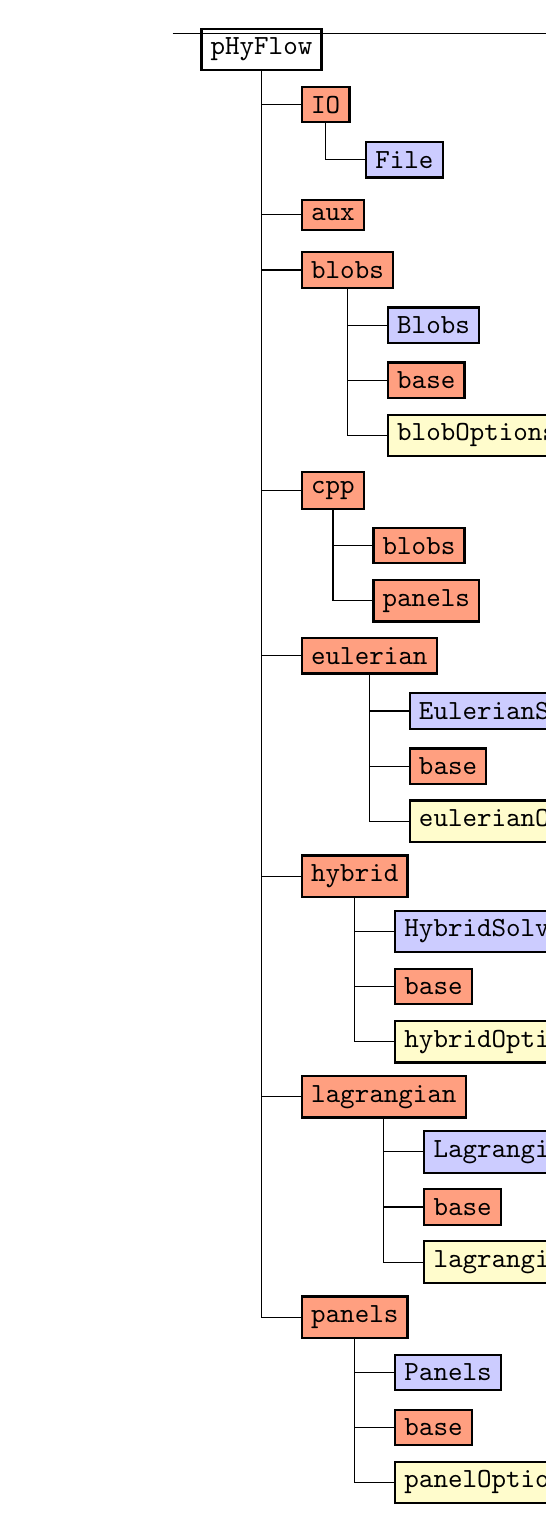
\begin{tikzpicture}[%
  grow via three points={one child at (0.5,-0.7) and
  two children at (0.5,-0.7) and (0.5,-1.4)},
  edge from parent path={(\tikzparentnode.south) |- (\tikzchildnode.west)}]
  \node {\texttt{pHyFlow}}
    child {node [module] {\texttt{IO}}
   		child {node [class] {\texttt{File}}}
   	%child {node {\texttt{cpp}}}  	
    }
    child [missing] {}    
    child {node [module] {\texttt{aux}}
   		%child {node {\texttt{File}}}
   	%child {node {\texttt{cpp}}}  	
    } 
    child {node [module] {\texttt{blobs}}
		child {node [class] {\texttt{Blobs}}}
		child {node [module] {\texttt{base}}}  	
		child {node [script] {\texttt{blobOptions}}}  	
    }    
    child [missing] {}				
    child [missing] {}				
    child [missing] {}    			
    child { node [module] {\texttt{cpp}}
		child {node [module] {\texttt{blobs}}}
		child {node [module] {\texttt{panels}}}
    	}
    child [missing] {}	
    child [missing] {}    			
    child { node [module] {\texttt{eulerian}}
		child {node [class] {\texttt{EulerianSolver}}}
		child {node [module] {\texttt{base}}}
		child {node [script] {\texttt{eulerianOptions}}}
    	}
    child [missing] {}				
    child [missing] {}	
    child [missing] {}    
    child { node [module] {\texttt{hybrid}}
		child {node [class]{\texttt{HybridSolver}}}
		child {node [module] {\texttt{base}}}
		child {node [script] {\texttt{hybridOptions}}}
    	}
    child [missing] {}					
    child [missing] {}	
    child [missing] {}    
    child { node [module] {\texttt{lagrangian}}
		child {node [class] {\texttt{LagrangianSolver}}}
		child {node [module] {\texttt{base}}}
		child {node [script] {\texttt{lagrangianOptions}}}
    	}
    child [missing] {}				
    child [missing] {}	       
    child [missing] {}	
    child { node [module] {\texttt{panels}}
		child {node [class] {\texttt{Panels}}}
		child {node [module] {\texttt{base}}}
		child {node [script] {\texttt{panelOptions}}}
    	};
\end{tikzpicture}
\caption{Flowchart of the \texttt{pHyFlow} library structured into \mybox[fill=orange!50!red!50!white]{modules}, \mybox[fill=yellow!20]{option} script files, and \mybox[fill=blue!20]{classes}.}
\label{fig:tikz_pHyFlowStructure}
\end{figure}

The \texttt{pHyFlow} library extends \python computing environment, where one can solve hybrid flow problems. To achieve this, we have implemented an Eulerian solver and a Lagrangian solver (without panel diffusion scheme, which can be used as a standalone solver for verification and validation). The \texttt{pHyFlow} library is structured into several modules, categorized by their purposes. In each \texttt{module}, we defined a \texttt{class} that handles the functions in the module. To add flexibility in computation, we added an \texttt{option} file where the user can change the solver's options. Figure \ref{fig:tikz_pHyFlowStructure} shows the structure of the \texttt{pHyFlow} library, classified using a color code. The structure of the \texttt{pHyFlow} is as follows:

\begin{itemize}
\item \texttt{IO}: This module contains all the input/output functions for saving and plotting data. The \texttt{File} class handles the functions of the \texttt{IO} module.
\item \texttt{aux}: This module contains all the auxiliary function of the library that does not belong to the fluid dynamics computation.
\item \texttt{cpp}: The module that contains all the low-level compiled functions that have been wrapped for the use in \textsf{python}. This module contains the two main low-level algorithms for performing the induced velocity calculations for vortex blobs and vortex panels, and the remeshing algorithm for the vortex blobs.
\item \texttt{blobs}: This module contains all the vortex blob related functions. Contains the class \texttt{Blobs} and the vortex blob solver object, handling all the vortex blobs operations. The algorithms of the vortex blobs defined in chapter \ref{ch:lagrangian} are implemented in this module.
\item \texttt{panels}: This module contains all the vortex panel functions and is wrapped in the class \texttt{Panels}. The algorithms of the vortex panel defined in chapter \ref{ch:lagrangian} are implemented in this module
\item \texttt{lagrangian}: This module contains all the vortex blob and vortex panel coupling functions. The vortex panel, vortex blob coupling algorithm described in chapter \ref{ch:lagrangian} is implemented in this module.
\item \texttt{eulerian}: This module contains all the Navier-Stokes grid operations. The algorithms explained in chapter \ref{ch:eulerian} are implemented in this module.
\item \texttt{hybrid}: This module contains all the functions related to coupling of the Lagrangian and the Eulerian solver, summarized in section \ref{sec:coupling-mlca}, \ref{sec:la-eolm}, and \ref{sec:eu-eotem}. The functions are wrapped in the \texttt{HybridSolver} class and manage the global coupling process.

\end{itemize}

Figure \ref{fig:tikz_pHyFlowStructure} shows the structure of the \texttt{pHyFlow} library and is categorized into several modules of different purposes. It is structured in this manner such that one could employ the library for any general simulation purpose such as the hybrid case, or for non-hybrid cases (e.g. potential flow using vortex panels, full Eulerian grid simulation using Eulerian solver). This means that one could use a single module of \texttt{pHyFlow} library for the desired test case.

\section{Hybrid class Hierarchy}

However, the hybrid module relies on the functions of the Lagrangian module and the Eulerian module. Moreover, the Lagrangian module requires the function of vortex blob module and the vortex panel module. Therefore, the hierarchy of the hybrid class is defined in a different manner, as shown in figure \ref{fig:tikz_hybridStructure}. 

\begin{figure}[h]
\centering
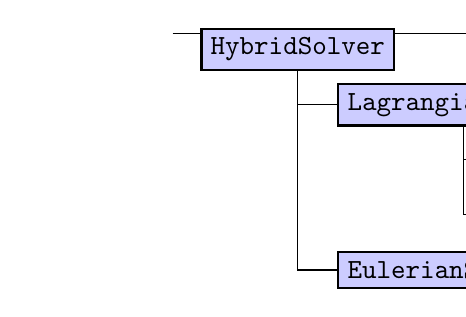
\begin{tikzpicture}[%
  grow via three points={one child at (0.5,-0.7) and
  two children at (0.5,-0.7) and (0.5,-1.4)},
  edge from parent path={(\tikzparentnode.south) |- (\tikzchildnode.west)}]
  \node [class] {\texttt{HybridSolver}}
    child {node [class] {\texttt{LagrangianSolver}}
   		child {node [class] {\texttt{Blobs}}}
   		child {node [class] {\texttt{Panels}}}
    }
    child [missing] {}    
    child [missing] {}    
    child {node [class] {\texttt{EulerianSolver}}};
\end{tikzpicture}
\caption{Flowchart of the \texttt{HybridSolver} hierarchy. The \texttt{HybridSolver} couples the \texttt{LagrangianSolver} class and the \texttt{EulerianSolver} class using the hybrid coupling schemes.}
\label{fig:tikz_hybridStructure}
\end{figure}

We use a bottom-up approach to construct the \texttt{HybridSolver} object, starting from the lower-level objects: \texttt{Blobs}, \texttt{Panels}. Then constructing the mid-level objects: \\ \texttt{LagrangianSolver}, and \texttt{EulerianSolver}. Finally constructing the highest-level object: \texttt{HybridSolver}. The procedure for constructing the hybrid class is as follows:
\begin{enumerate}
	\item Construct the lowest-level objects:
		\begin{enumerate}
		\item Construct the \texttt{Blobs} object using the vorticity field parameters, the vortex blob parameters, time step parameters, and population control parameters.
		\item Construct the \texttt{Panels} object using panel geometry parameters.
		\end{enumerate}

	\item Construct the mid-level solvers:
		\begin{enumerate}
		\item Construct \texttt{LagrangianSolver} object using the vortex blob object \texttt{Blobs} and the vortex panel object \texttt{Panels}.
		\item Construct \texttt{EulerianSolver} object using the geometry mesh file, interpolation probe grid parameters, and the fluid parameters.
		\end{enumerate}
		
	\item Construct the hybrid solver:
		\begin{enumerate}
		\item Construct \texttt{HybridSolver} object using the Lagrangian solver object \\ \texttt{LagrangianSolver}, the Eulerian solver object \texttt{EulerianSolver}, and the interpolation parameters.
		\end{enumerate}

\end{enumerate}		

A detailed description of the parameters required for the construction of the objects, and the schematic of these objects are given in appendix \ref{app:code}.

%  	% Chapter 7: Verification and Validation of the Hybrid Method
	\chapter{Verification and Validation of Hybrid Method}
\label{ch:vavohm}

This chapter focuses on the verification and the validation of the hybrid method. To perform this feat, we investigated several test-cases: Lamb-Oseen Vortex at $Re=1000$, Clercx-Bruneau Dipole collision at $Re=625$, Impulsively Started Cylinder at $Re=1000$ and the flow around an elliptical airfoil at $Re=5000$.

The verification of \texttt{pHyFlow} was perform as a start where we used the analytical solution of the Lamb-Oseen vortex to verify the velocity and the vorticity field. The Lamb-Oseen vortex problem was also essential for investigating the influences of the solver parameters that impact the accuracy of the coupling. 

The validation of the accuracy of the hybrid solver was performed, once we verified the proper implementation of the hybrid solver. Clercx-Bruneau dipole collision test case was used to investigate the generation of the vorticity in the hybrid scheme and the transfer of this vorticity. This was the first test-cases, where we could confirm the implementation of the vortex panel for the hybrid scheme.


%\section{Comparison of Eulerian vs. Lagrangian solution}
%
%\subsection{Comparison of vorticity contours}
%
%\subsection{Error in maximum vorticity}t
%
%\subsection{Error in $L^2$-norm of velocity}
%
%\subsection{Error in $L^2$-norm of vorticity}

\section{Lamb-Oseen Vortex Evolution}

The Lamb-Oseen Vortex test case simulates the evolution of a laminar vortex core in an unbounded domain. In section \ref{subsec:lagrangianLambOseen}, we used this test case to verify and validate the implementation of the vortex blobs of the Lagrangian solver and in section \ref{subsec:eulerianLambOseen}, we used it to verify the implementation of the Eulerian solver. Therefore, in a similar fashion we will employ this test case to verify the coupling of the hybrid solver. 

The unbounded nature of the problem helps us to neglect the influence of the solid boundary (i.e the wall). Therefore, this test case does not require the panel solver in the Lagrangian solver as we are only concerned with the coupling of the vortex blobs to the Eulerian solver. Thus, we can primarily focus of the vorticity field interpolation error discussed in section \ref{subsubsec:vfie}, and quantitatively present the importance of ensuring conservation of circulation. This is the primary purpose of employing the Lamb-Oseen Vortex test case.

The secondary purpose is to quantify the influences of the discretization on the accuracy of the coupling. A parameter sensitivity analysis was therefore performed to determine their effects on the coupling error. The parameters that determine the spatial discretization of the vortex blobs is nominal particle spacing $h$, and the overlap ratio $Ov$ (see figure \ref{fig:blobOverlap}). The spatial discretization of the Eulerian solver is regarded as a control variable for this test case as its impact was concluded in section \ref{subsec:eulerianLambOseen}. The parameters that determine the temporal discretization of the hybrid method is the time step size of the Eulerian solver $\Delta t_E$ and the time step size of the Lagrangian solver $\Delta t_L$ which are depended according to equation \ref{eq:timeStepDependency} where $k_E$ is the number of Eulerian sub-steps.

The coupling error was quantified my determining the growth of maximum relative error in vorticity $\epsilon$ given by equation \ref{eq:maxRelErrorDef}, approach used in section \ref{subsec:lagrangianLambOseen} and section \ref{subsec:eulerianLambOseen}. 


\subsection{Problem Definition}

The Lamb-Oseen Vortex problem is defined by the vorticity field, equation \ref{eq:lo_voeq}, and the velocity field, equation \ref{eq:lo_veeq}. The hybrid solver is initialized by first assigning the strengths of the vortex blobs using equation \ref{eq:lo_pie}. The Eulerian domain $\Omega_E$ is then initialized using the solution of the Lagrangian solver. Daeninck \cite{Daeninck2006} used this approach to enhance the coupling between the methods ensuring minimum interpolation error.

	\ctable[
		caption = {Summary of the parameters for the Lamb-Oseen vortex evolution. Parameters tabulated below are used for benchmark case.},
		label   = {tab:HLO_pt},
		pos = t,]{lcll}{}{\FL
		
		Parameters 					& Value 	& Unit					& Description \ML
		$\Gamma_c$\T               	& 1 &\si{m^2.s^{-1}} 				& Core strength\\
		$\Omega$               		& $[-0.5,0.5]\times[-0.5,0.5]$ &\si{m}		& Eulerian domain bounds \\
		$\nu$						& $0.001$ &\si{kg.s^{-1}.m^{-1}}& Kinematic viscosity\\
		$ \tau$ 		    		& $100$ 	&\si{s}	& Initial time\\
		$Ov$						& 1 & - & Overlap ratio\\
		$h$							& 0.01 & \si{m} & Nominal blob spacing\\
		$\Gamma_{thres}$			& (\num{1e-14}, \num{1e-14}) & - & Population Control threshold\\
		$h_{grid}$ 					& \numrange{0.007}{0.016} & \si{m} & FE cell diameter span \\
		$ N_{\mathrm{cells}}$ 		& $26448$ 	& -						& Number of mesh cells\\
		$\Delta t_L$				& 0.001 & \si{s} & Lagrangian time step size\\
		$\Delta t_E$				& 0.001 & \si{s} & Eulerian time step size\\		
		$k_E$						& 1 & - & Eulerian sub-steps\\
		$ N_{\mathrm{t-steps}}$ 	& 1000 & -				& Number of time integration steps\\
		$t$ 		    			& \numrange{0}{1} 	&\si{s}			& Simulation time span\\		
		$d_{bdry}$					& $2\cdot{h}$ & \si{m} & Interpolation boundary offset\LL}

	\begin{figure}[h]
	\showthe\columnwidth
	\centering
	\includegraphics[width=0.5\linewidth]{./figures/hybrid/lambOseen/hlo_dd-crop.pdf}
	\caption{The domain decomposition for the Lamb-Oseen vortex problem, $\Omega_E \subseteq \Omega_L$. The Eulerian domain bounds $\Omega_E = [-1,1]\times[-1,1]$ with Dirichlet boundary $\partial \Omega_{dirichlet}$ [{\color{plotRed}{---}}, solid red] (\emph{not to scale}).}
	\label{fig:HLO_dc}
	\end{figure}

Figure \ref{fig:HLO_dc} shows the Hybrid domain configuration for the Lamb-Oseen Vortex problem with the Lagrangian domain $\Omega_L$ spanning the full fluid domain. The Eulerian domain $\Omega_E$ only resolves the center of the Lamb-Oseen core, $\Omega_E \subseteq \Omega_L$. The domain bounds $[-0.5,-0.5] \times [-0.5,-0.5]$ with a Dirichlet velocity boundary $\Sigma_d$ where the velocity boundary condition is applied as described in section 
\ref{subsec:dbc}. The correction of the Lagrangian domain is performed in the interpolation domain $\Omega_{int}$ according to the procedures described in section \ref{sec:correction}.

The spatial discretization of the Eulerian domain $\Omega_E$ is regarded as the control variable. Therefore, the parameter sensitivity analysis is performed by varying the spatial discretization of the Lagrangian method. The Eulerian domain is discretized with an unstructured mesh formulation using GMSH (see section \ref{subsec:mgugmsh}) having $N_{cells} = 226448$ unstructured cells and grid size $h_{grid}$ spanning $0.007$ to $0.0016$. 

The Lamb-Oseen Vortex problem is defined according to the parameters tabulated in table \ref{tab:HLO_pt}. The core is located at $(0,0)$, where the Eulerian domain $\Omega_E$ is centered. The parameters are chosen such that vorticity $\omega$ and velocity $\mathbf{u}$ is non-zero at the boundary of the Eulerian domain $\Sigma_d$, figure \ref{fig:HLO_dc}. 

The evolution of the Lagrangian solver and the Eulerian solver is performed according to section \ref{sec:evolveLagrangian} and \ref{sec:evolveEulerian} respectively. The Lagrangian solver performs TRS for diffusion of the vortex blobs, see section \ref{subsubsec:srs}. The scheme requires vortex blob redistribution at every step, $f_{redis} = 1$. In conjunction with the redistribution, the population control is performed at every step, $f_{pc}=1$ with $\Gamma_{thre}$ in table \ref{tab:HLO_pt}. 


\subsection{Results and Discussion}

The investigation of the Lamb-Oseen vortex problem is divided into three parts. The first part of the investigation concerns with comparing several stages of the hybrid coupling, section \ref{subsec:UvOvF}, where we compare the uncoupled scheme with the one-way coupled scheme and fully coupled scheme. These successive coupling investigate will help determine the source and quantify the error of the coupling. The second part of the investigation, section \ref{subsubsec:coc} focuses on importance of conservation of circulation that was discussed in section \ref{subsubsec:cc}. The results of the non-conserved and conserved scheme are compared to conclude the importance of conservation of circulation. During these two investigations, the parameters tabulated in table \ref{tab:HLO_pt} are used.

The third and final investigation is dedicated to the parameter sensitivity analysis, section \ref{subsubsec:psa}. Parameters that determine the spatial and temporal discretization of the scheme is investigated to verify the convergence of scheme.

\subsection{Uncoupled vs. One-way Coupled vs. Fully Coupled}
\label{subsec:UvOvF}
To verify the implementation of the hybrid algorithm, we compared several stages of the hybrid coupling with the standard, fully Eulerian test case. The three types of the coupling are as given:

\begin{itemize}
\item \textbf{Uncoupled}: The uncoupled test case involves only Eulerian solver and serves as a benchmark to quantify the error in coupling. The boundary conditions are determined directly from the analytical formulation, equation 	\ref{eq:eLO_veq}.
\item \textbf{One-way coupled}: The one-way coupled test case is a partially coupled hybrid test case where the Eulerian method is evolved using the Lagrangian solution. The correction of the Lagrangian solution is not performed in this scenario. Thus, this case will help us determine the error in evolution Eulerian method using the Lagrangian solution.
\item \textbf{Fully coupled}: The fully coupled test case performs the full coupling strategy described in section \ref{subsec:mcs}. The Eulerian method is evolved using the Lagrangian solution and the Lagrangian solution in the interpolation domain $\Omega_{int}$, figure \ref{fig:HLO_dc} is corrected at the end of each time step. This test case will help us quantify the error in transferring the Eulerian solution to the Lagrangian method.
\end{itemize}
	
	\begin{figure}[h]
     \centering
     \begin{subfigure}[t]{0.45\textwidth}
             \includegraphics[width=\linewidth]{./figures/hybrid/lambOseen/lambOseen_fully_vErrorInitial_raster.pdf}
             \caption{Velocity}
             \label{fig:lambOseen_oneway_vErrorInitial}
     \end{subfigure}%
     \qquad %add desired spacing between images, e. g. ~, \quad, \qquad etc.
       %(or a blank line to force the subfigure onto a new line)
     \begin{subfigure}[t]{0.45\textwidth}
             \includegraphics[width=\linewidth]{./figures/hybrid/lambOseen/lambOseen_fully_wErrorInitial_compressed.pdf}
             \caption{Vorticity}
             \label{fig:lambOseen_uncoupled_wErrorInitial}
     \end{subfigure}
     \caption{Initial relative error at $t=0$ inside the Eulerian domain. The figure depicts \textbf{(a)} the relative error in velocity $\mathbf{u}$ and \textbf{(b)} the relative error in vorticity $\omega$.}
     \label{fig:lambOseen_initialError}
	\end{figure}
		
Figure \ref{fig:lambOseen_initialError} depicts the initial relative error in velocity and vorticity inside the Eulerian domain $\Omega_E$. The relative error in velocity is near machine epsilon $\epsilon \le \num{10e-8}$, but the error in vorticity is in the order \num{10e-5}. Similar observation was made in section \ref{subsec:eulerianLambOseen} and arises from the projection error when determining the vorticity from velocity. The error is dependent on the type of discretization and we have second-order velocity space and first-order vorticity space. 

	\begin{figure}[!t]
	\centering
	\includegraphics[width=0.6\linewidth]{./figures/hybrid/lambOseen/lambOseen_comparision_compressed.pdf}
	\caption{Comparison of the evolution of the maximum relative error from $t=0$ to $t=1$. The figure compares standard case (\textbf{black}) vs. the one-way coupled case ({\color{plotBlue}{\textbf{blue}}}) vs. the fully coupled case ({\color{plotRed}{\textbf{red}}}). The plot depicts maximum relative error in velocity (dashed), and the maximum relative error in vorticity (solid).}
	\label{fig:lambOseen_comparison}
	\end{figure}

The simulation is evolved from $t=0$ to $t=1$ with $N_{t-steps} = 1000$ Lagrangian and Eulerian time steps using the time step parameters tabulated in table \ref{tab:HLO_pt}. Figure \ref{fig:lambOseen_comparison} shows the evolution of maximum relative error in vorticity $\omega$ and velocity $\mathbf{u}$ of the uncoupled, one-way coupled and the fully coupled cases in the Eulerian domain $\Omega_E$ w.r.t. the analytical solution, equation \ref{eq:lo_voeq}. The initial observation shows the error in velocity is two to three orders of magnitude less than the error in vorticity and occurs due to the projection error. The figure shows that the uncoupled scheme has the lowest error in vorticity and velocity. As the boundary condition is directly obtained from the analytical solution, the error only arises from FE discretization of the Eulerian method. As time progresses, the error in velocity converges around \num{10e-7} and the error in vorticity converges around \num{10e-4}.

The one-way coupled case shows an increase in the velocity field inside the Eulerian domain $\Omega_E$. The increase in error is negligible at the initial stages of the coupling. This states that the discretization error of the analytical solution is well represented using the vortex blobs. At $t=1$, the error in velocity increases by two orders of magnitude from \num{10e-7} to \num{10e-5}. This implies that the error is due to the growth in error of the Lagrangian field. In chapter \ref{ch:lagrangian}, we observed there is an increase in the error due to the circulation processing techniques (population control, remeshing) and the time-marching of the vortex blobs.

The fully coupled case demonstrates that there is further increase in the error in velocity. Moreover, we observe that the there is now an increase in error in vorticity as well. As we are transfer the discrete vorticity field from the Eulerian method to the Lagrangian method it causes an increase in error of the Lagrangian solution. The consequence of this is that now the velocity field resolved by the Lagrangian method has an addition error. The figure depicts this effect, showing an increase in error in velocity. After the first few iteration (around $t=0.2$), there is a measurable difference between the fully coupled and the one-way coupled case. 

	
	\begin{figure}[h]
     \centering
     \begin{subfigure}[t]{0.45\textwidth}
             \includegraphics[width=\linewidth]{./figures/hybrid/lambOseent2/lambOseen_uncoupled_vErrorFinal_compressed-crop.pdf}
             \caption{Standard; velocity $\mathbf{u}$}
             \label{fig:lambOseen_uncoupled_vErrorFinal}
     \end{subfigure}%
     \qquad %add desired spacing between images, e. g. ~, \quad, \qquad etc.
       %(or a blank line to force the subfigure onto a new line)
     \begin{subfigure}[t]{0.45\textwidth}
             \includegraphics[width=\linewidth]{./figures/hybrid/lambOseent2/lambOseen_uncoupled_wErrorFinal_compressed-crop.pdf}
             \caption{Standard; vorticity $\omega$}
             \label{fig:lambOseen_uncoupled_wErrorFinal}
     \end{subfigure}%       
       
     \begin{subfigure}[t]{0.45\textwidth}
             \includegraphics[width=\linewidth]{./figures/hybrid/lambOseent2/lambOseen_oneway_vErrorFinal_compressed-crop.pdf}
             \caption{One-way coupled; velocity $\mathbf{u}$}
             \label{fig:lambOseen_oneway_vErrorFinal}
     \end{subfigure}
     \qquad
     \begin{subfigure}[t]{0.45\textwidth}
             \includegraphics[width=\linewidth]{./figures/hybrid/lambOseent2/lambOseen_oneway_wErrorFinal_compressed-crop.pdf}
             \caption{One-way coupled; vorticity $\omega$}
             \label{fig:lambOseen_oneway_wErrorFinal}
     \end{subfigure}     
   
     \begin{subfigure}[t]{0.45\textwidth}
             \includegraphics[width=\linewidth]{./figures/hybrid/lambOseent2/lambOseen_fully_vErrorFinal_compressed-crop.pdf}
             \caption{Fully coupled; velocity $\mathbf{u}$}
             \label{fig:lambOseen_fully_vErrorFinal}
     \end{subfigure}     
     \qquad
     \begin{subfigure}[t]{0.45\textwidth}
             \includegraphics[width=\linewidth]{./figures/hybrid/lambOseent2/lambOseen_fully_wErrorFinal_compressed-crop.pdf}
             \caption{Fully coupled; vorticity $\omega$}
             \label{fig:lambOseen_fully_wErrorFinal}
     \end{subfigure}        
     
     \caption{Initial relative error at $t=0$ inside the Eulerian domain. The figure depicts \textbf{(a)} the relative error in velocity $\mathbf{u}$ and \textbf{(b)} the relative error in vorticity $\omega$.}
     \label{fig:lambOseen_finalError}
	\end{figure}	


\subsubsection*{Conservation of circulation}
\label{subsubsec:coc}

	\begin{figure}[h]
     \centering
     \begin{subfigure}[t]{0.45\textwidth}
             \includegraphics[width=\linewidth]{./figures/hybrid/lambOseent2/lambOseen_fully_vErrorFinal_compressed-crop.pdf}
             \caption{Conservation \texttt{on}; velocity $\mathbf{u}$}
             \label{fig:lambOseen_fullyCon_vErrorFinal}
     \end{subfigure}%
     \qquad %add desired spacing between images, e. g. ~, \quad, \qquad etc.
       %(or a blank line to force the subfigure onto a new line)
     \begin{subfigure}[t]{0.45\textwidth}
             \includegraphics[width=\linewidth]{./figures/hybrid/lambOseent2/lambOseen_fullyCoff_vErrorFinal_compressed-crop.pdf}
             \caption{Conservation \texttt{off}; velocity $\mathbf{u}$}
             \label{fig:lambOseen_fullyCoff_vErrorFinal}
     \end{subfigure}
     
    \begin{subfigure}[t]{0.45\textwidth}
             \includegraphics[width=\linewidth]{./figures/hybrid/lambOseent2/lambOseen_fully_wErrorFinal_compressed-crop.pdf}
             \caption{Conservation \texttt{on}; vorticity $\omega$}
             \label{fig:lambOseen_fullyCon_wErrorFinal}
     \end{subfigure}%         
     \qquad     
     \begin{subfigure}[t]{0.45\textwidth}
             \includegraphics[width=\linewidth]{./figures/hybrid/lambOseent2/lambOseen_fullyCoff_wErrorFinal_compressed-crop.pdf}
             \caption{Conservation \texttt{off}; vorticity $\omega$}
             \label{fig:lambOseen_fullyCoff_wErrorFinal}
     \end{subfigure}  

           
  
     \caption{Initial relative error at $t=0$ inside the Eulerian domain. The figure depicts \textbf{(a)} the relative error in velocity $\mathbf{u}$ and \textbf{(b)} the relative error in vorticity $\omega$.}
     \label{fig:lambOseen_conservation_contourf}
	\end{figure}


	\begin{figure}[h]
     \centering
     \begin{subfigure}[t]{0.45\textwidth}
             \includegraphics[width=\linewidth]{./figures/hybrid/lambOseent2/lambOseen_comparision_conservation_compressed.pdf}
             \caption{Relative Error in velocity and vorticity}
             \label{fig:lambOseen_comparision_conservation}
     \end{subfigure}%
     \qquad %add desired spacing between images, e. g. ~, \quad, \qquad etc.
       %(or a blank line to force the subfigure onto a new line)
     \begin{subfigure}[t]{0.45\textwidth}
             \includegraphics[width=\linewidth]{./figures/hybrid/lambOseent2/lambOseen_comparision_conservation_circulation_compressed.pdf}
             \caption{Error in total circulation $\Gamma$}
             \label{fig:lambOseen_comparision_conservation_circulation}
     \end{subfigure}%       
     \caption{Initial relative error at $t=0$ inside the Eulerian domain. The figure depicts \textbf{(a)} the relative error in velocity $\mathbf{u}$ and \textbf{(b)} the relative error in vorticity $\omega$.}
     \label{fig:lambOseen_conservation_comparisions}
	\end{figure}


\subsubsection{Parameter sensitiviy analysis}
\label{subsubsec:psa}

\subsection{Conclusion}



\section{Clercx-Bruneau Dipole Collision}

\subsection{Problem Definition}

\subsection{Results}

\subsection{Conclusion}

%
%\section{Clercx-Bruneau Dipole Collision}
%
%\subsection{Problem Definition}
%
%\subsection{Results}
%
%\subsection{Conclusion}

%
%	\begin{figure}[h]
%     \centering
%     \begin{subfigure}[t]{0.45\textwidth}
%             \includegraphics[width=\linewidth]{./figures/hybrid/lambOseen_standard_vErrorInitial_compressed-crop.pdf}
%             \caption{Velocity}
%             \label{fig:lambOseen_standard_vErrorInitial}
%     \end{subfigure}%
%     \qquad %add desired spacing between images, e. g. ~, \quad, \qquad etc.
%       %(or a blank line to force the subfigure onto a new line)
%     \begin{subfigure}[t]{0.45\textwidth}
%             \includegraphics[width=\linewidth]{./figures/hybrid/lambOseen_standard_wErrorInitial_compressed-crop.pdf}
%             \caption{Final Error}
%             \label{fig:lambOseen_standard_wErrorInitial}
%     \end{subfigure}
%     \caption{Initial Error of the Lamb-Oseen vortex}
%     \label{fig:lambOseen_initialError}
%	\end{figure}
%	
	

%	\begin{figure}[h]
%     \centering
%     \begin{subfigure}[t]{0.45\textwidth}
%             \includegraphics[width=\linewidth]{./figures/hybrid/lambOseen_vErrorInitial_compressed-crop.pdf}
%             \caption{Initial Error}
%             \label{fig:lambOseen_vErrorInitial_compressed-crop}
%     \end{subfigure}%
%     ~ %add desired spacing between images, e. g. ~, \quad, \qquad etc.
%       %(or a blank line to force the subfigure onto a new line)
%     \begin{subfigure}[t]{0.45\textwidth}
%             \includegraphics[width=\linewidth]{./figures/hybrid/lambOseen_vErrorFinal_k1_compressed-crop.pdf}
%             \caption{Final Error}
%             \label{fig:lambOseen_vErrorFinal_k1_compressed}
%     \end{subfigure}
%     \caption{Growth in error, velocity max. relative error, dtl=dte, h=0.02, dte=0.001}
%     \label{fig:lambOseen_vError}
%	\end{figure}
%	
%	\begin{figure}[h]
%     \centering
%     \begin{subfigure}[t]{0.45\textwidth}
%             \includegraphics[width=\linewidth]{./figures/hybrid/lambOseen_wErrorInitial_compressed-crop.pdf}
%             \caption{Initial Error}
%             \label{fig:lambOseen_wErrorInitial_compressed}
%     \end{subfigure}%
%     ~ %add desired spacing between images, e. g. ~, \quad, \qquad etc.
%       %(or a blank line to force the subfigure onto a new line)
%     \begin{subfigure}[t]{0.45\textwidth}
%             \includegraphics[width=\linewidth]{./figures/hybrid/lambOseen_wErrorFinal_k1_compressed-crop.pdf}
%             \caption{Final Error}
%             \label{fig:lambOseen_wErrorFinal_k1_compressed}
%     \end{subfigure}
%     \caption{Growth in error, vorticity max. relative error, dtl=dte, h=0.02, dte=0.001}
%     \label{fig:lambOseen_wError}
%	\end{figure}	
	
\subsection{Variation in Lagrangian time step size}	
	
%	\begin{figure}[h]
%		\centering
%		\begin{subfigure}[t]{0.45\textwidth}
%		      \includegraphics[width=\linewidth]{./figures/hybrid/lambOseen_vErrorFinal_k1_compressed-crop.pdf}
%		      \caption{$k=1$}
%		      \label{fig:lambOseen_vErrorFinal_k1}
%		\end{subfigure}%
%		~ %add desired spacing between images, e. g. ~, \quad, \qquad etc.
%		%(or a blank line to force the subfigure onto a new line)
%		\begin{subfigure}[t]{0.45\textwidth}
%		      \includegraphics[width=\linewidth]{./figures/hybrid/lambOseen_vErrorFinal_k2_compressed-crop.pdf}
%		      \caption{$k=2$}
%		      \label{fig:lambOseen_vErrorFinal_k2}
%		\end{subfigure}
%		~
%		\begin{subfigure}[t]{0.45\textwidth}
%		      \includegraphics[width=\linewidth]{./figures/hybrid/lambOseen_vErrorFinal_k5_compressed-crop.pdf}
%		      \caption{$k=5$}
%		      \label{fig:lambOseen_vErrorFinal_k5}
%		\end{subfigure}		
%		~
%		\begin{subfigure}[t]{0.45\textwidth}
%		      \includegraphics[width=\linewidth]{./figures/hybrid/lambOseen_vErrorFinal_k10_compressed-crop.pdf}
%		      \caption{$k=5$}
%		      \label{fig:lambOseen_vErrorFinal_k10}
%		\end{subfigure}			
%		
%		\caption{Variation in the Lagrangian k, velocity max. relative error, dtl=k*dte, h=0.02, dte=0.001}
%		\label{fig:lambOseen_vError_k}
%	\end{figure}
%	
%	
%	\begin{figure}[h]
%		\centering
%		\begin{subfigure}[t]{0.45\textwidth}
%		      \includegraphics[width=\linewidth]{./figures/hybrid/lambOseen_wErrorFinal_k1_compressed-crop.pdf}
%		      \caption{$k=1$}
%		      \label{fig:lambOseen_wErrorFinal_k1}
%		\end{subfigure}%
%		~ %add desired spacing between images, e. g. ~, \quad, \qquad etc.
%		%(or a blank line to force the subfigure onto a new line)
%		\begin{subfigure}[t]{0.45\textwidth}
%		      \includegraphics[width=\linewidth]{./figures/hybrid/lambOseen_wErrorFinal_k2_compressed-crop.pdf}
%		      \caption{$k=2$}
%		      \label{fig:lambOseen_wErrorFinal_k2}
%		\end{subfigure}
%		~
%		\begin{subfigure}[t]{0.45\textwidth}
%		      \includegraphics[width=\linewidth]{./figures/hybrid/lambOseen_wErrorFinal_k5_compressed-crop.pdf}
%		      \caption{$k=5$}
%		      \label{fig:lambOseen_wErrorFinal_k5}
%		\end{subfigure}		
%		~
%		\begin{subfigure}[t]{0.45\textwidth}
%		      \includegraphics[width=\linewidth]{./figures/hybrid/lambOseen_wErrorFinal_k10_compressed-crop.pdf}
%		      \caption{$k=5$}
%		      \label{fig:lambOseen_wErrorFinal_k10}
%		\end{subfigure}			
%		
%		\caption{Variation in the Lagrangian k, velocity max. relative error, dtl=k*dte, h=0.02, dte=0.001}
%		\label{fig:lambOseen_wError_k}
%	\end{figure}		
	
	
%	\begin{figure}[h]
%	\centering
%	\includegraphics[width=0.5\linewidth]{./figures/hybrid/daeninck_CylinderVorticity.png}
%	\caption{Result of hybrid coupling by Daeninck \cite{Daeninck2006}. The figure shows artificial vorticity at the boundary of the Eulerian domain.}
%	\label{fig:daeninck_CylinderVorticity}
%	\end{figure}




\section{Error in coupling: Verification with Lamb-Oseen vortex}

	\subsection{Generation of artificial vorticity}


\section{Clercx-Bruneau dipole convection at $Re=625$}

	\subsection{Comparison of vorticity contours}
	
	\subsection{Variation in maximum vorticity}
	
	\subsection{Variation in kinetic energy}
	
	\subsection{Variation in enstrophy}

\section{Clercx-Bruneau dipole collision at $Re=625$}

	\subsection{Comparison of vorticity contours}
	
	\subsection{Variation in maximum vorticity}
	
	\subsection{Variation in kinetic energy}
	
	\subsection{Variation in Enstrophy}
	
	\subsection{Variation in Palinstrophy}

\section{Impulsively started cylinder problem at $Re=550$}

	\subsection{Evolution of the wake}
	
	\subsection{Evolution of pressure and friction drag}
	
	\subsection{Evolution of lift}

\section{Moving body}

	\subsection{Error due to pertubation lag}

\section{Proof of concepts}

	\subsection{Multiple cylinder case}
	
	\subsection{Stalled airfoil at $Re=5000$}

\section{Summary}   

%   	% Chapter 8: Conclusion and Recommendations
   \chapter{Conclusion and Recommendation}
\label{ch:ConclusionandRecommendation}

\section{Conclusion}

\subsection{Lagrangian domain}

\subsection{Eulerian domain}

\subsection{Hybrid method}

%\subsection{Feasibility of hybrid vortex method for compressor cascade}

\section{Recommendations}

\subsection{Lagrangian domain}

\subsection{Eulerian domain}

\subsection{Hybrid method}

%\subsection{RBF kernel representation of boundary}
%
%\subsection{Recommended numerical simulation for compressor cascade}

    
    % Bibliography
    \printbib{bibliography/library,bibliography/others}
    
    % and some appendices here
    %\addcontentsline{toc}{chapter}{Appendix}
    \appendix  
%    \chapter{Coordinate Systems}


%		\subsection{Coordinate Systems}
%			% Coordinate system: local to global transformation.
%			% summarize: coordinates systems of panels, lagrangian, eulerian
%			% how is the body defined? How it the problem constructed? 
%
    
\chapter{\texttt{pHyFlow} Code Structure}
\label{app:code}%

% Tikz stypes
\tikzstyle{every node}=[draw=black,thick,anchor=west]
\tikzstyle{optional}=[dashed,fill=gray!20]
\tikzstyle{selected}=[draw=red,fill=red!30]


%\title{pHyFlow Code Structure}
%\author{Artur Palha, Lento Manickathan}

%\begin{document}
%\maketitle
%\begin{abstract}
The document outlines the \texttt{pHyFlow} code structure. The \texttt{pHyFlow} functions are organized into several classes. The functions related to the vortex particles are placed inside the \texttt{Blobs} class. The functions related to the panel problem are inside \texttt{Panels} class. The \texttt{LagrangianSolver} class is made to couple the functions of the vortex blobs and the vortex panel together. The functions of the Eulerian domain are placed inside the \texttt{EulerianSolver} class, where the Navier-stokes grid problem is solved. Finally, coupling of all the problems are done with the \texttt{HybridSolver} class. Note, all the classes are capable of handling multi-body / multi-domain problem within them and \texttt{LagrangianSolver} class and the \texttt{HybridSolver} class only couples methods together.\\

\underline{\texttt{pHyFlow} Structure:}
\begin{figure}[h]
\centering
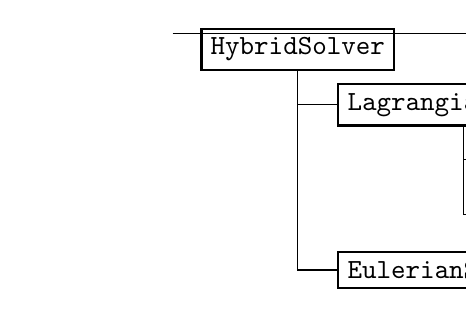
\begin{tikzpicture}[%
  grow via three points={one child at (0.5,-0.7) and
  two children at (0.5,-0.7) and (0.5,-1.4)},
  edge from parent path={(\tikzparentnode.south) |- (\tikzchildnode.west)}]
  \node {\texttt{HybridSolver}}
    child { node {\texttt{LagrangianSolver}}
    	child {node {\texttt{Blobs}}}
    	child {node {\texttt{Panels}}}  	
    }
    child [missing] {}				
    child [missing] {}				
    child { node {\texttt{EulerianSolver}}};
    %child { node [selected] {tex}
    %  child { node {generic}}
    %  child { node [optional] {latex}}
    %  child { node {plain}}
    %}
    %child [missing] {}
    %child { node {texdoc}};
\end{tikzpicture}
\end{figure}
%\end{abstract}
\newpage

\section*{\texttt{Blobs} Class}
The main structure of the \texttt{Blobs} class. This class contains all the function related to the calculation of the vortex blobs.
\begin{figure}[h]
\centering
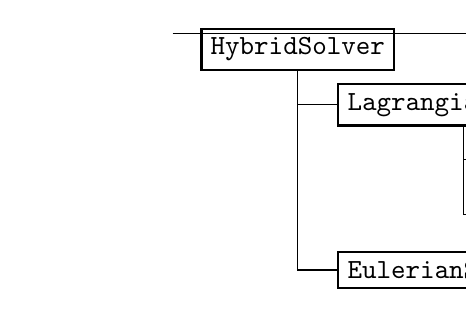
\begin{tikzpicture}[%
  grow via three points={one child at (0.5,-0.7) and
  two children at (0.5,-0.7) and (0.5,-1.4)},
  edge from parent path={(\tikzparentnode.south) |- (\tikzchildnode.west)}]
  \node {\texttt{HybridSolver}}
    child { node {\texttt{LagrangianSolver}}
    	child {node [selected] {\texttt{Blobs}}}
    	child {node {\texttt{Panels}}}  	
    }
    child [missing] {}				
    child [missing] {}				
    child { node {\texttt{EulerianSolver}}};
    %child { node [selected] {tex}
    %  child { node {generic}}
    %  child { node [optional] {latex}}
    %  child { node {plain}}
    %}
    %child [missing] {}
    %child { node {texdoc}};
\end{tikzpicture}
\end{figure}

\subsection*{Class structure:}
\begin{figure}[h]
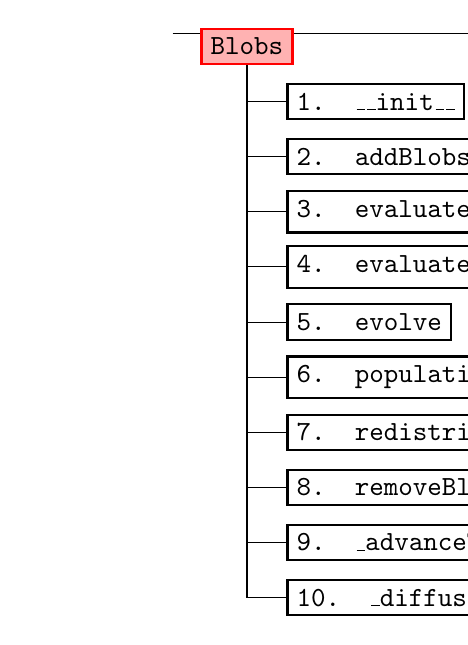
\begin{tikzpicture}[%
  grow via three points={one child at (0.5,-0.7) and
  two children at (0.5,-0.7) and (0.5,-1.4)},
  edge from parent path={(\tikzparentnode.south) |- (\tikzchildnode.west)}]
  \node [selected] {\texttt{Blobs}}
    child { node {\texttt{1. \_\_init\_\_}}}
    child { node {\texttt{2. addBlobs}}}
    child { node {\texttt{3. evaluateVelocity}}}                    
    child { node {\texttt{4. evaluateVorticity}}}   
    child { node {\texttt{5. evolve}}}    
    child { node {\texttt{6. populationControl}}}   
    child { node {\texttt{7. redistribute}}}    
	child { node {\texttt{8. removeBlobs}}}  
	child { node {\texttt{9. \_advanceTime}}}  	
	child { node {\texttt{10. \_diffusion}}};	
\end{tikzpicture}
\end{figure}

\subsection*{Attributes:}
\begingroup
\footnotesize
\begin{longtable}{|l|p{9cm}|}
	\hline
	\textbf{Attributes} & \textbf{Description}\\
	\toprule
    \texttt{blobControlParams} 		& The diffusion parameters. It is a dictionary containing all the parameters of the diffusion method used for the simulation. Contains: \texttt{stepRedistribution}, \texttt{stepPopulationControl}, \texttt{gThresholdLocal}, \texttt{gThresholdGlobal}.\\\hline
    \texttt{computationMethod} 		&\texttt{computationMethod} (tuple) with the type of Biot-Savart solver (\texttt{direct}, \texttt{fmm}) and the type of hardware to use (\texttt{cpu}, \texttt{gpu}).\\\hline
    \texttt{deltaTc} & The size of the convective time step $\Delta t_c$\\\hline
    \texttt{deltaTd} & The size of the convective time step $\Delta t_d$\\\hline
    \texttt{diffusionParams} & A dictionary containing all the parameters related to the computation of the diffusion step. Specifies the diffusion scheme and other specific parameters. Contains: \texttt{method}, \texttt{c2}.\\\hline
    \texttt{g} & The strength of the vortex blobs $\alpha$.\\          \hline
    \texttt{gThresholdGlobal} & Maximum value of variation of total vorticity due to the removal of blobs during population control.\\\hline
    \texttt{gThresholdLocal} & Minimum value of circulation to consider for each vortex blob when selecting blobs to remove during population control.\\    \hline      
    \texttt{h} & The size of the cell associated to the vortex blobs. Corresponds to the minimum spacing between the core of two neighboring cells. It is related to the core size of the blob, $\sigma$, and to the spacing $h$ by the expression $Ov = h/\sigma$.\\\hline          
    \texttt{integrationMethod} & \texttt{integrationMethod} (\texttt{fe}, \texttt{rk4}) the type of time integrator used: \texttt{fe} forward Euler, \texttt{rk4} Runge-Kutta $4^{th}$ order.\\ \hline
    \texttt{nu} & The fluid kinematic viscosity, used to calculate the diffusion coefficient: \texttt{c2} and diffusion time step \texttt{deltaTd}, $\Delta t_{d}$.\\          \hline
	\texttt{numBlobs} & The number of blobs.\\          \hline
	\texttt{overlap} & The overlap ratio between neighboring blobs.\\          \hline
	\texttt{plotVelocity} & A flag that defines if velocity is to be plotted or not.\\          \hline
	\texttt{sigma} & The core size of the vortex blobs.\\          \hline
	\texttt{stepDiffusion} & The frequency of diffusion steps.\\          \hline
	\texttt{stepPopulationControl} & The frequency of population control.\\          \hline
	\texttt{stepRedistribution} & The frequency of redistribution of blobs.\\          \hline
	\texttt{timeIntegrationParams} & A dictionary containing all time integration parameters of the simulation. Contains the definition of the time integration scheme possibly additional parameters specific to the scheme.\\ \hline
	\texttt{t} & The current time of the simulation.\\          \hline
	\texttt{tStep} & The current time step of the simulation.\\          \hline
	\texttt{velocityComputationParams} & A dictionary containing all the parameters related to the computation of induced velocities. Specifies computation scheme (direct or fmm) and hardware to use (cpu or gpu).\\          \hline
	\texttt{vInf} & The free stream velocity.\\          \hline
	\texttt{x} & The $x$ coordinates of the vortex blobs.\\          \hline
	\texttt{y} & The $y$ coordinates of the vortex blobs.\\          \hline	                                
    
                       
    \caption{Attributes of \texttt{Blobs} class and their description.}
    \label{tab:attributeBlobs}
\end{longtable}
\endgroup

\subsection*{\texttt{\_\_init\_\_}}
	\paragraph{Description:} Initialize the \texttt{Blobs} class with either the given input parameters or by a reading a \texttt{file} containing all the necessary parameters.\\
	
	\begin{tabular}{l|lp{7cm}}
		\multicolumn{2}{l}{\textbf{Input Parameters}} & \\ \hline
		\textit{File Name} & \multicolumn{2}{l}{Containing all the parameters to re-initalize the class.} \\ \cline{2-3}
		\multicolumn{3}{c}{--- or ---} \\ \cline{2-3}
		\multirow{4}{*}{\textit{Parameters}} & Vorticity Field &: \{\texttt{xBlob, yBlob, gBlob}\} or \{\texttt{wFunction, xBounds, yBounds}\}\\ \cline{2-3}
		& Blob parameters &: \texttt{overlap, h} \\ \cline{2-3}
		& Time Step parameters &: \texttt{deltaTc, nu, stepRedistribution, integrationMethod, computationMethod}\\ \cline{2-3}
		& Population control parameters &: \texttt{stepPopulationControl, gThreshold}\\ \cline{2-3}
	\end{tabular}\\
	
	\subsubsection*{Descriptions of the parameters:}
	\begin{tabular}{p{3.5cm}p{9cm}p{1cm}}
				\textit{Vorticity field} & & \textit{Default}\\ \hline
				\texttt{xBlob,yBlob} &:  the $x,y$ blob coordinates. & - \\
				\texttt{gBlob} &: the circulation $\Gamma_i$ associated to each of the vortex blobs. & - \\
				& & \\
				\multicolumn{2}{c}{\textit{--- or ---}} & \\
				& & \\
				\texttt{wExactFunction} &: the function that returns the exact value of vorticity $\omega$ at any given $x,y$ coordinates. &\\
				& 	\begin{tabular}{lp{10cm}}
						\textbf{Input parameters} &: \texttt{xEval,yEval}\\ 
						\textbf{Assigns} &: \texttt{-}\\ 			
						\textbf{Returns} &: \texttt{wEval}\\ 					
					\end{tabular} & - \\
				\texttt{xBounds, yBounds} &: the $x,y$ bounds of the domain where the particles was originally distributed. & - \\		 
	\end{tabular}\\
	\\ \\
	%	\begin{tabular}{lp{10cm}}
	%		\textbf{Input parameters} &: \texttt{xEval,yEval}\\ 
	%		\textbf{Assigns} &: \texttt{-}\\ 			
	%		\textbf{Returns} &: \texttt{vortEval}\\ 					
	%	\end{tabular}\\
	\begin{tabular}{p{3.5cm}p{9cm}p{1cm}}
				\multicolumn{2}{l}{\textit{Blob parameters}} & \textit{Default} \\ \hline				
				\texttt{overlap} &: the overlap ratio $h/\sigma$. & 1.0\\
				\texttt{h} &: the size of the cell $h$ associated to the blobs. \textit{Note:} Cells are square. & -\\
	\end{tabular}\\
	\\ \\
	\begin{tabular}{p{3.5cm}p{9cm}p{1cm}}
				\multicolumn{2}{l}{\textit{Time step parameters}} & \textit{Default}\\ \hline
				\texttt{deltaTc} &:  the size of the convective time step $\Delta t_c$. & - \\
				\texttt{nu} &: the fluid kinematic viscosity $\nu$, used to calculate the diffusion coefficient $c^2$ and diffusion time step size $\Delta T_d$.& - \\
				\texttt{stepRedistribution} &: the redistribution step frequency. & 1 \\
				\texttt{integrationMethod} &: the time integration method (\texttt{FE}: Forward euler , \texttt{RK4}: $4^{th}$ order Runge-Kutta). & RK4 \\
				\texttt{computationMethod} &: the calculation method to evolve the blobs, (\texttt{Direct}: Direct Method, \texttt{FMM}: Fast-Multipole Method) using (\texttt{CPU}, \texttt{GPU}). & \{FMM, GPU\}.\\
	\end{tabular}\\ 
    \\ \\ 
	\begin{tabular}{p{3.5cm}p{9cm}p{1cm}}
				\multicolumn{2}{l}{\textit{Population control parameters}} & \textit{Default} \\ \hline
				\texttt{stepPopulationControl} &: population control step frequency & 1.\\
				\texttt{gThreshold} &: the tuple with minimum \textbf{and} maximum value of the circulation $\Gamma_{min}$. & - \\
	\end{tabular}\\ 
    \\ \\  
	\begin{tabular}{p{3.5cm}p{9cm}p{1cm}}
				\multicolumn{2}{l}{\textit{Free stream velocity}} & \textit{Default}\\ \hline
				\texttt{vInf} &: The free-stream velocity function, returning the velocity action on the vortex blobs. & -\\		
				&		\begin{tabular}{lp{2cm}}
							\textbf{Input parameters} &: \texttt{t}\\ 
							\textbf{Assigns} &: \texttt{-}\\ 			
							\textbf{Returns} &: \texttt{vx,vy}\\ 					
						\end{tabular} & - \\
				
	\end{tabular}\\

\newpage
%%%%%%%%%%%%%%%%%%%%%%%%%%%%%%%%%%%%%%%%%%%%%%%%%%%%%%%%%%%%%%%%%%%%%%%%%%%%%%%%%%%%%%%%%%%%%%%%%%%%%%%%%%%%%%%%%%%%%%%%%%%%%%%%%%
%%%%%%%%%%%%%%%%%%%%%%%%%%%%%%%%%%%%%%%%%%%%%%%%%%%%%%%%%%%%%%%%%%%%%%%%%%%%%%%%%%%%%%%%%%%%%%%%%%%%%%%%%%%%%%%%%%%%%%%%%%%%%%%%%%

\section*{\texttt{Panels} class}
The main structure of the panel method class \texttt{Panels}. This class contains all the functions related to the calculation of panels.

\begin{figure}[h]
\centering
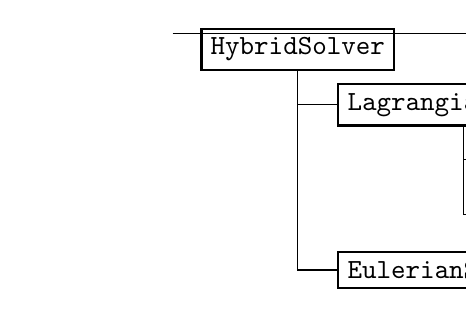
\begin{tikzpicture}[%
  grow via three points={one child at (0.5,-0.7) and
  two children at (0.5,-0.7) and (0.5,-1.4)},
  edge from parent path={(\tikzparentnode.south) |- (\tikzchildnode.west)}]
  \node {\texttt{HybridSolver}}
    child { node {\texttt{LagrangianSolver}}
    	child {node {\texttt{Blobs}}}
    	child {node [selected] {\texttt{Panels}}}  	
    }
    child [missing] {}				
    child [missing] {}				
    child { node {\texttt{EulerianSolver}}};
    %child { node [selected] {tex}
    %  child { node {generic}}
    %  child { node [optional] {latex}}
    %  child { node {plain}}
    %}
    %child [missing] {}
    %child { node {texdoc}};
\end{tikzpicture}
\end{figure}


\subsection*{Class structure:}
\begin{figure}[h]
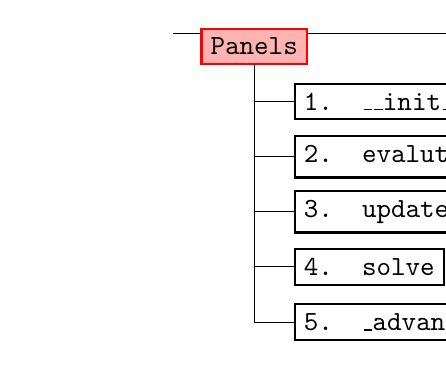
\begin{tikzpicture}[%
  grow via three points={one child at (0.5,-0.7) and
  two children at (0.5,-0.7) and (0.5,-1.4)},
  edge from parent path={(\tikzparentnode.south) |- (\tikzchildnode.west)}]
  \node [selected] {\texttt{Panels}}
    child { node {\texttt{1. \_\_init\_\_}}}
    child { node {\texttt{2. evaluteVelocity}}}                    
    child { node {\texttt{3. updateBody}}}                    
    child { node {\texttt{4. solve}}}                                        
    child { node {\texttt{5. \_advanceTime}}};
\end{tikzpicture}
\end{figure}


\subsection*{Attributes:}
\begingroup
\footnotesize
\begin{longtable}{|l|p{11cm}|}
	\hline
	\textbf{Attributes} & \textbf{Description}\\
	\toprule
    \texttt{A} 		& The inter-induction matrix $\mathbf{A}$, the LHS of the problem. \\ \hline
    \texttt{cmGlobal} & The global position vector for each of the $\mathbf{N}$
                       body, refining the position of the local panel $(0,0)$ in the
                       global coordinate system. \\\hline
    \texttt{deltaT} & The simulation time step size $\Delta T$\\ \hline
    \texttt{geometryKeys} & The dictionary containing all the parameters of the geometry. Contains: \texttt{xPanel} (the $x$ coordinate of the $\mathbf{M}$ panel corners.), \texttt{yPanel} (The $y$ coordinate of the $\mathbf{M}$ panel corners), \texttt{cmGlobal}, \texttt{thetaLocal}, \texttt{dPanel} (The off-set of the panel collocation point from the panel mid-point).  \\ \hline
    \texttt{nBodies} & The number of panel bodies.\\\hline
    \texttt{norm} & The $x$, $y$ normal vector of each panel.\\\hline
    \texttt{normCat} & The global concatenated $x$, $y$ component of the panel normal vector at each collocation points.\\          \hline
    \texttt{nPanels} & The number of panels in each body/geometry. \\ \hline
    \texttt{nPanelsTotal} & The total number of panels.\\    \hline      
    \texttt{panelKernel} & A string defining panel kernel type. \\\hline          
    \texttt{problemType} & A string defining the panel problem is of a \texttt{moving} type or of a \texttt{fixed} type.\\ \hline
    \texttt{solverCompParams} & The dictionary containing solver computation parameters.\\          \hline
	\texttt{sPanel} & The vortex sheet strengths $\gamma$ of $\mathbf{M}$ panels. \\          \hline
	\texttt{t} & The current time $t$ of the simulation.\\          \hline
	\texttt{tang} & The $x$, $y$ tangent vector of each panel.\\          \hline
	\texttt{tangCat} & The global concatenated $x$, $y$ component of the panel
	                  normal vector at each collocation points.\\          \hline
	\texttt{thetaLocal} & The local rotation angle $\theta$ w.r.t to the local
	                     coordinate system. The rotational will be performed around
	                     the local reference point $(0,0)$, i.e around the global center of rotation point \texttt{cmGlobal}.\\          \hline
	\texttt{tStep} & The current step of the simulation.\\          \hline
	\texttt{velCompParams} & A dictionary containing the velocity computation parameters, method and hardware.\\          \hline
	\texttt{xyCPGlobal} & The global $x$, $y$ coordinate of the panel collocation
	                     points.\\ \hline
	\texttt{xyCPGlobalCat} & The global concatenated $x$, $y$ coordinate of the
	                        panel collocation points.\\          \hline
	\texttt{xyPanelGlobal} & The global $x$, $y$ coordinate of the panel bodies.\\          \hline
	\texttt{xyPanelGlobalCat} & The global concatenated $x$, $y$ coordinate of the
	                           panel bodies.\\          \hline
	\texttt{xyPanelLocal} & The local $x$, $y$ coordinate of the panel bodies.\\          \hline
                       
    \caption{Attributes of \texttt{Panels} class and their description.}
    \label{tab:attributesPanels}
\end{longtable}
\endgroup


\subsection*{\texttt{\_\_init\_\_}}
	\begin{tabular}{l|lp{7cm}}
		\multicolumn{2}{l}{\textbf{Input Parameters}} & \\ \hline
		\textit{File Name} & \multicolumn{2}{l}{Containing all the parameters to re-initalize the class.} \\ \hline
		\multirow{2}{*}{\textit{Parameters}} & Panel coordinates &: \{\texttt{xCP, yCP, xPanel, yPanel, cmGlobal, thetaLocal}\}\\ \cline{2-3}
		& External velocity &: \texttt{externVel} \\ \cline{2-3}
	\end{tabular}
	\paragraph{Description:} Initialize the \texttt{panels} class with the given input parameters. In the case of a multibody problem, a list of panel coordinates can be given and internally it takes care of the inter-coupling.\\
	\\
	\begin{tabular}{lp{10cm}}
				\textit{Panel coordinates} & \\ \hline
				\texttt{xCP,yCP} &:  the local $x,y$-coordinates of the panel collocation points.\\ 
				\texttt{xPanel,yPanel} &: the local coordinate of the panel edges. \textit{Note}: Should have a closed loop (end with initial point coordinates).\\ 
				\texttt{cmGlobal} &:  the position of reference points of a given panel body.\\
				\texttt{thetaLocal} &:  the rotational angles of the panel body axes w.r.t to the global $x$-axis.\\
	\end{tabular}\\ 
    \\ \\
	\begin{tabular}{lp{10cm}}
				\textit{External velocity} & \\ \hline
				\texttt{externVel} &:  Reference to an external velocity \textbf{function} acting of the panels. For the panel case, the external velocity will the induced velocity of the blobs + freestream \texttt{vortexBlob.evaluateVelocity}.\\
	\end{tabular}\\
	
		\begin{tabular}{lp{10cm}}
			\textbf{Input parameters} &: \texttt{xCP,yCP}\\ 
			\textbf{Assigns} &: \texttt{-}\\ 			
			\textbf{Returns} &: \texttt{vxCP,vyCP}\\ 					
		\end{tabular}\\


\newpage
%%%%%%%%%%%%%%%%%%%%%%%%%%%%%%%%%%%%%%%%%%%%%%%%%%%%%%%%%%%%%%%%%%%%%%%%%%%%%%%%%%%%%%%%%%%%%%%%%%%%%%%%%%%%%%%%%%%%%%%%%%%%%%%%%%
%%%%%%%%%%%%%%%%%%%%%%%%%%%%%%%%%%%%%%%%%%%%%%%%%%%%%%%%%%%%%%%%%%%%%%%%%%%%%%%%%%%%%%%%%%%%%%%%%%%%%%%%%%%%%%%%%%%%%%%%%%%%%%%%%%

\section*{\texttt{LagrangianSolver} Class}
The main structure of the \texttt{Blobs} + \texttt{Panels} (LagrangianSolver) class. This class contains all the function related to the calculations of panel with vortex blobs.

\begin{figure}[h]
\centering
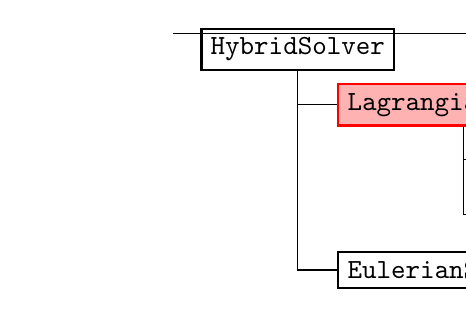
\begin{tikzpicture}[%
  grow via three points={one child at (0.5,-0.7) and
  two children at (0.5,-0.7) and (0.5,-1.4)},
  edge from parent path={(\tikzparentnode.south) |- (\tikzchildnode.west)}]
  \node {\texttt{HybridSolver}}
    child { node [selected] {\texttt{LagrangianSolver}}
    	child {node {\texttt{Blobs}}}
    	child {node {\texttt{Panels}}}  	
    }
    child [missing] {}				
    child [missing] {}				
    child { node {\texttt{EulerianSolver}}};
    %child { node [selected] {tex}
    %  child { node {generic}}
    %  child { node [optional] {latex}}
    %  child { node {plain}}
    %}
    %child [missing] {}
    %child { node {texdoc}};
\end{tikzpicture}
\end{figure}

\subsection*{Class structure:}
\begin{figure}[h]
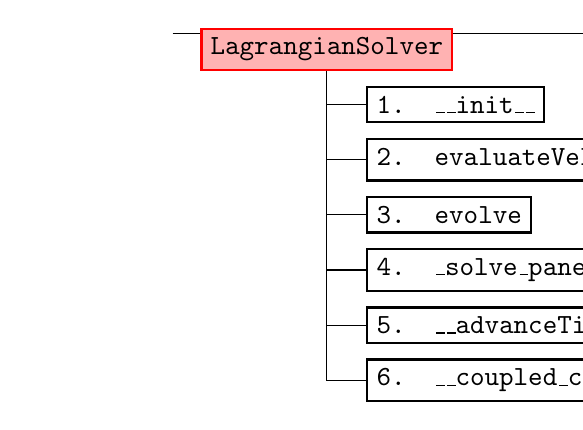
\begin{tikzpicture}[%
  grow via three points={one child at (0.5,-0.7) and
  two children at (0.5,-0.7) and (0.5,-1.4)},
  edge from parent path={(\tikzparentnode.south) |- (\tikzchildnode.west)}]
  \node [selected] {\texttt{LagrangianSolver}}
    child { node {\texttt{1. \_\_init\_\_}}}
    child { node {\texttt{2. evaluateVelocity}}}
    child { node {\texttt{3. evolve}}}
    child { node {\texttt{4. \_solve\_panelStrength}}}                        
    child { node {\texttt{5. \_\_advanceTime}}}                        
    child { node {\texttt{6. \_\_coupled\_convection}}};                       

\end{tikzpicture}
\end{figure}

\subsection*{Attributes:}
\begingroup
\footnotesize
\begin{longtable}{|l|p{12cm}|}
	\hline
	\textbf{Attributes} & \textbf{Description}\\
	\toprule
    \texttt{deltaT}     & The inter-induction matrix $\mathbf{A}$, the LHS of the problem. \\ \hline
    \texttt{gTotal}     & The total circulation of the Lagrangian domain. \\ \hline    
	\texttt{t} & The current time $t$ of the simulation.\\          \hline
	\texttt{tStep} & The current step of the simulation.\\          \hline
	\texttt{vInf} & The $x$, $y$ component of the free-stream velocity.\\          \hline	
	\texttt{Blobs} & The vortex blobs class \texttt{Blobs}.\\          \hline	
	\texttt{Panels} & The vortex panels class \texttt{Panels}.\\          \hline			
                      
    \caption{Attributes of \texttt{LagrangianSolver} class and their description.}
    \label{tab:attributesLagrangianSolver}
\end{longtable}
\endgroup


\subsection*{\texttt{\_\_init\_\_}}
	\begin{tabular}{l|lp{7cm}}
		\multicolumn{2}{l}{\textbf{Input Parameters}} & \\ \hline
		\textit{File Name} & \multicolumn{2}{l}{Containing all the parameters to re-initalize the class.} \\ \hline
		\multirow{2}{*}{\textit{Parameters}} & \texttt{vortexBlobs} &: \{\texttt{vortexBlobs}\} class. \\ \cline{2-3}
		& \texttt{panels} &: \texttt{panels} class. \\ \cline{2-3}
	\end{tabular}
	\paragraph{Description:} Initialize the \texttt{vortexMethod} class using \textbf{vortexBlob}+\textbf{panelMethod} \\ classes.
	\paragraph{Input parameters:}
	\begin{list}{\quad}{}
	\item \texttt{Blobs}: vortex particle class
	\item \texttt{Panels}: panel method class				
	\end{list}


\newpage
%%%%%%%%%%%%%%%%%%%%%%%%%%%%%%%%%%%%%%%%%%%%%%%%%%%%%%%%%%%%%%%%%%%%%%%%%%%%%%%%%%%%%%%%%%%%%%%%%%%%%%%%%%%%%%%%%%%%%%%%%%%%%%%%%%
%%%%%%%%%%%%%%%%%%%%%%%%%%%%%%%%%%%%%%%%%%%%%%%%%%%%%%%%%%%%%%%%%%%%%%%%%%%%%%%%%%%%%%%%%%%%%%%%%%%%%%%%%%%%%%%%%%%%%%%%%%%%%%%%%%

\section*{\texttt{EulerianSolver}}
The main structure for the Navier-stokes class \texttt{EulerianSolver}. This class contains all the functions related to computation of the Navier-stokes problem. Below is set of functions that acts as the interface to the class.

\begin{figure}[h]
\centering
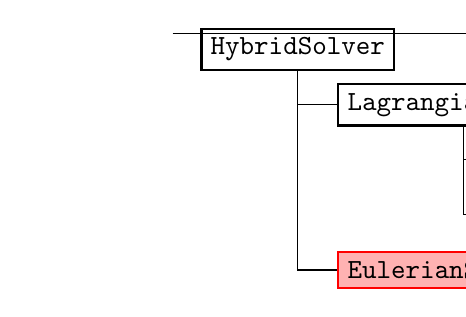
\begin{tikzpicture}[%
  grow via three points={one child at (0.5,-0.7) and
  two children at (0.5,-0.7) and (0.5,-1.4)},
  edge from parent path={(\tikzparentnode.south) |- (\tikzchildnode.west)}]
  \node {\texttt{HybridSolver}}
    child { node {\texttt{LagrangianSolver}}
    	child {node {\texttt{Blobs}}}
    	child {node {\texttt{Panels}}}  	
    }
    child [missing] {}				
    child [missing] {}				
    child { node [selected] {\texttt{EulerianSolver}}};
    %child { node [selected] {tex}
    %  child { node {generic}}
    %  child { node [optional] {latex}}
    %  child { node {plain}}
    %}
    %child [missing] {}
    %child { node {texdoc}};
\end{tikzpicture}
\end{figure}



\subsection*{Class structure:}
\begin{figure}[h]
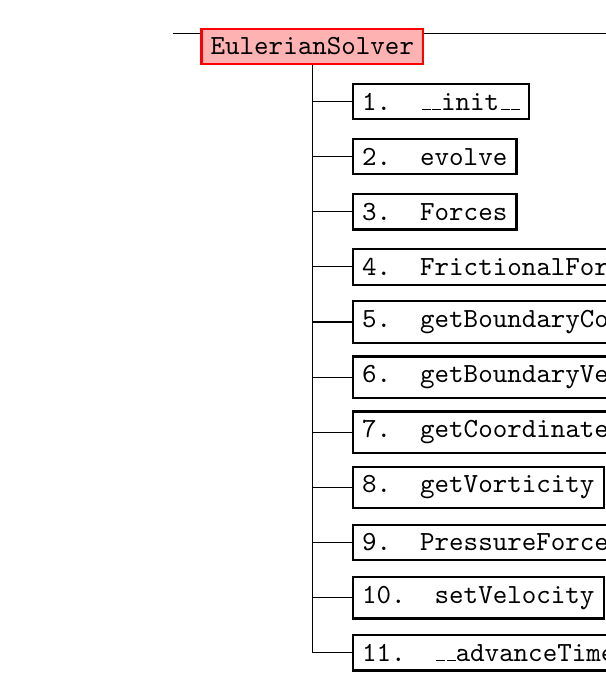
\begin{tikzpicture}[%
  grow via three points={one child at (0.5,-0.7) and
  two children at (0.5,-0.7) and (0.5,-1.4)},
  edge from parent path={(\tikzparentnode.south) |- (\tikzchildnode.west)}]
  \node [selected] {\texttt{EulerianSolver}}
    child { node {\texttt{1. \_\_init\_\_}}}
    child { node {\texttt{2. evolve}}}
    child { node {\texttt{3. Forces}}}
    child { node {\texttt{4. FrictionalForces}}}
    child { node {\texttt{5. getBoundaryCoordinates}}}                            
    child { node {\texttt{6. getBoundaryVelocity}}}                    
    child {node  {\texttt{7. getCoordinates}}}            
    child { node {\texttt{8. getVorticity}}}                                   
    child { node {\texttt{9. PressureForces}}}
    child { node {\texttt{10. setVelocity}}}
    child { node {\texttt{11. \_\_advanceTime}}};
\end{tikzpicture}
\end{figure}


\subsection*{Attributes:}
\begingroup
\footnotesize
\begin{longtable}{|l|p{11cm}|}
	\hline
	\textbf{Attributes} & \textbf{Description}\\
	\toprule
    \texttt{deltaT} 		& The time step size $\Delta t$. \\ \hline
    \texttt{deltaTMax} 		& The maximum allowable time step size $\max\{\Delta t\}$.\\ \hline
    \texttt{cfl} 			& The Courant–Friedrichs–Lewy condition stability number CFL. \\ \hline        
    \texttt{cmGlobal} 		& The $x$, $y$ position of the mesh local reference point $(0,0)$ in the global coordinates. \\ \hline        
    \texttt{hMin} 			& The minimum mesh cell size. \\ \hline        
    \texttt{nu} 			& The fluid kinematic viscosity $\nu$.  \\ \hline        
    \texttt{probeGridMesh} 	& The \textit{local} $x$, $y$ coordinates of the probe grid mesh. \\ \hline            
    \texttt{probeGridParams}& The dictionary containing all the parameters of the probe grid for extracting the vorticity data. \\ \hline            
    \texttt{solverParams} 	& The dictionary file containing all the solver parameters.  \\ \hline                
    \texttt{t} 				& The current time of the simulation. \\ \hline                    
    \texttt{thetaLocal} 	& The local rotational angle $\theta$ of the mesh domain. Therefore, the rotation will be done about local reference  point $(0,0)$, i.e \texttt{cmGlobal} in the global coordinate system.\\ \hline                            
    \texttt{tStep} 			& The current step of the simulation. \\ \hline                    
    \texttt{uMax} 			& The maximum fluid velocity $\max\{\mathbf{u}\}$. \\ \hline
    
    \caption{Attributes of \texttt{EulerianSolver} class and their description.}
    \label{tab:attributeEulerian}
\end{longtable}
\endgroup


\subsection*{\texttt{\_\_init\_\_}}
	\paragraph{Description:} Initialize the \texttt{navierStokes} class either using a \texttt{fileName} containing all the necessary parameter for initialization or by explicitly inputing the parameters.\\

	\begin{tabular}{l|lp{7cm}}
		\multicolumn{2}{l}{\textbf{Input Parameters}} & \\ \hline
		\textit{File Name} & \multicolumn{2}{l}{Containing all the parameters to re-initalize the class.} \\ \hline
		\multicolumn{3}{c}{-- or --} \\ \hline
		\multirow{5}{*}{\textit{Parameters}} & Mesh data &: \texttt{mesh, boundaryDomains}\\ \cline{2-3}
		& Geometry position &: \texttt{cmGlobal, thetaLocal} \\ \cline{2-3}
		& Fluid parameters &: \texttt{uMax, nu}\\ \cline{2-3}
		& Solver options &: \texttt{cfl}\\ \cline{2-3}
		& Probe grid parameters &: \texttt{x0, y0, Lx, Ly, hx, hy}\\ \cline{2-3}

	\end{tabular}\\
	\subsubsection*{Description of the parameters:}
	
	\begin{tabular}{lp{10cm}}
				\textit{Mesh data} & \\ \hline
				\texttt{mesh} &: the mesh data file.\\ 
				\texttt{boundaryDomains} &: the boundary mesh domain data file.\\ 			
	\end{tabular}\\ 
    \\ \\
	\begin{tabular}{lp{10cm}}
				\textit{Geometry position} & \\ \hline
				\texttt{cmGlobal} &: the $x,y$ position of the geometry in global coordinates.\\ 
				\texttt{thetaGlobal} &: the rotation angle (in $rad$) of the geometry in global coordinate system.\\ 			
	\end{tabular}\\
    \\ \\
	\begin{tabular}{lp{10cm}}
				\textit{Fluid parameters} & \\ \hline
				\texttt{uMax} &: the maximum fluid velocity $U_{max}$. Used to determine the maximum time step size $\Delta t_{max}$.\\ 
				\texttt{nu} &: the fluid kinematic viscosity $\nu$, for incompressible navier-stokes problem.\\ 			
	\end{tabular}\\	
    \\ \\
	\begin{tabular}{lp{10cm}}
				\textit{Solver options} & \\ \hline
				\texttt{cfl} &: the $CFL$ stability parameter. If explicit time marching scheme, $CFL<1$.\\ 		
	\end{tabular}\\	
    \\ \\
	\begin{tabular}{lp{10cm}}
				\textit{Probe grid parameters} & \\ \hline
				\texttt{x0,y0} &: the $x,y$ coordinate of the origin of the probe grid.\\ 
				\texttt{Lx,Ly} &: the $x,y$ size (width and height) of the probing grid.\\ 			
				\texttt{hx,hy} &: the $x,y$ spacing of the probe grid cell.\\ 							
	\end{tabular}\\	


\newpage
%%%%%%%%%%%%%%%%%%%%%%%%%%%%%%%%%%%%%%%%%%%%%%%%%%%%%%%%%%%%%%%%%%%%%%%%%%%%%%%%%%%%%%%%%%%%%%%%%%%%%%%%%%%%%%%%%%%%%%%%%%%%%%%%%%
%%%%%%%%%%%%%%%%%%%%%%%%%%%%%%%%%%%%%%%%%%%%%%%%%%%%%%%%%%%%%%%%%%%%%%%%%%%%%%%%%%%%%%%%%%%%%%%%%%%%%%%%%%%%%%%%%%%%%%%%%%%%%%%%%%


\section*{\texttt{HybridSolver} Class}
The main structure for the hybrid class \texttt{HybridSolver}. This class contains all the functions related to computation of the hybrid problem.

\begin{figure}[h]
\centering
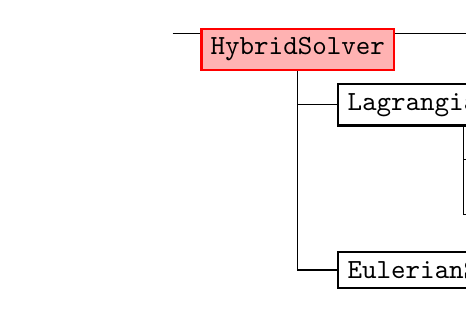
\begin{tikzpicture}[%
  grow via three points={one child at (0.5,-0.7) and
  two children at (0.5,-0.7) and (0.5,-1.4)},
  edge from parent path={(\tikzparentnode.south) |- (\tikzchildnode.west)}]
  \node [selected] {\texttt{HybridSolver}}
    child { node {\texttt{LagrangianSolver}}
    	child {node {\texttt{Blobs}}}
    	child {node {\texttt{Panels}}}  	
    }
    child [missing] {}				
    child [missing] {}				
    child { node {\texttt{EulerianSolver}}};
    %child { node [selected] {tex}
    %  child { node {generic}}
    %  child { node [optional] {latex}}
    %  child { node {plain}}
    %}
    %child [missing] {}
    %child { node {texdoc}};
\end{tikzpicture}
\end{figure}

\subsection*{Class structure:}
\begin{figure}[h]
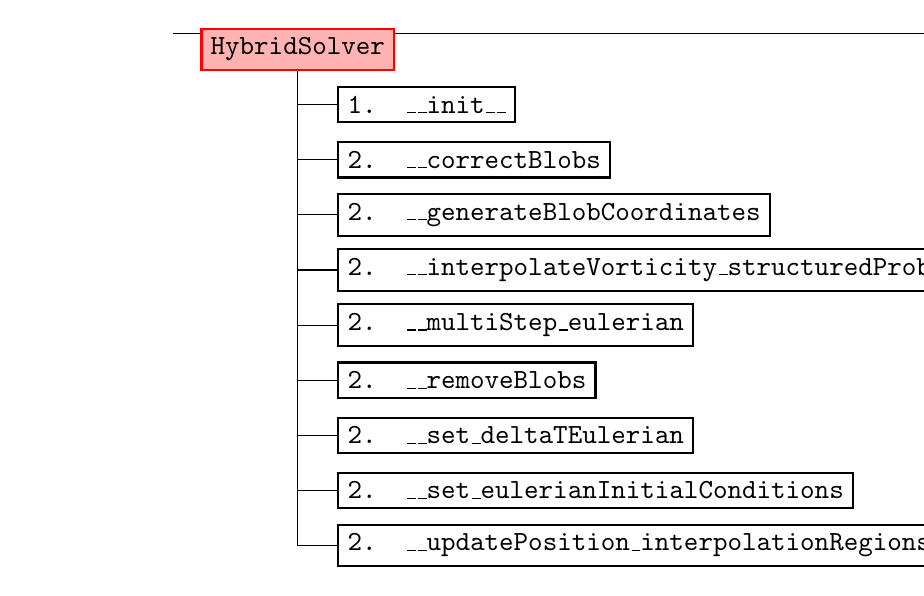
\begin{tikzpicture}[%
  grow via three points={one child at (0.5,-0.7) and
  two children at (0.5,-0.7) and (0.5,-1.4)},
  edge from parent path={(\tikzparentnode.south) |- (\tikzchildnode.west)}]
  \node [selected] {\texttt{HybridSolver}}
    child { node {\texttt{1. \_\_init\_\_}}}
    child { node {\texttt{2. \_\_correctBlobs}}}
    child { node {\texttt{2. \_\_generateBlobCoordinates}}}
    child { node {\texttt{2. \_\_interpolateVorticity\_structuredProbes\_manual}}}
    child { node {\texttt{2. \_\_multiStep\_eulerian}}}
    child { node {\texttt{2. \_\_removeBlobs}}}
    child { node {\texttt{2. \_\_set\_deltaTEulerian}}}    
    child { node {\texttt{2. \_\_set\_eulerianInitialConditions}}}        
    child { node {\texttt{2. \_\_updatePosition\_interpolationRegions}}};
\end{tikzpicture}
\end{figure}


\subsection*{Attributes:}
\begingroup
\footnotesize
\begin{longtable}{|l|p{10cm}|}
	\hline
	\textbf{Attributes} & \textbf{Description}\\
	\toprule
    \texttt{deltaTEulerian} 		& The time step size of the Eulerian sub-domain $\Delta t_E$. \\ \hline
    \texttt{deltaTLagrangian} 		& The time step size of the Lagrangian sub-domain $\Delta t_L$.\\ \hline
	\texttt{nu} 			& The fluid kinematic viscosity $\nu$.  \\ \hline        
    \texttt{t} 				& The current time $t$ of the simulation. \\ \hline                    
    \texttt{tStep} 			& The current step of the simulation. \\ \hline                    
    \texttt{vInf} 			& The $x$, $y$ component of the free-stream velocity. \\ \hline
    \texttt{interpolationRegion} & The dictionary containing the \texttt{surfacePolygon} and \texttt{boundaryPolygon} defining the boundaries of the interpolation region for each Eulerian sub-domains. The geometry is identified by the keys of the Eulerian sub-domain found in \texttt{multiEulerian}. The coordinates are defined in local coordinate system of the Eulerian grid and will be transformed (rotated + moved) during the evolution step. \\ \hline
    \texttt{lagrangian} 	& The Lagrangian solver class contains all the parameters related to simulation the flow in lagrangian sub-domain. \\ \hline
    \texttt{multiEulerian} 	& The \texttt{multiEulerian} is solver class containing all the Eulerian sub-domains of the hybrid problem. \\ \hline
    
    \caption{Attributes of \texttt{HybridSolver} class and their description.}
    \label{tab:attributeHybrid}
\end{longtable}
\endgroup


\subsection*{\texttt{\_\_init\_\_}}
	\begin{tabular}{l|lp{7cm}}
		\multicolumn{2}{l}{\textbf{Input Parameters}} & \\ \hline
		\textit{File Name} & \multicolumn{2}{l}{Containing all the parameters to re-initalize the class.} \\ \hline
		\multirow{4}{*}{\textit{Parameters}} & \texttt{vortexMethod} &: \{\texttt{vortexMethod}\} class.\\ \cline{2-3}
		& \texttt{navierStokes} &: \texttt{navierStokes} class. \\ \cline{2-3}
		& Interpolation region &: \texttt{xPolygon, yPolygon}\\ \cline{2-3}
		& Motion functions &: \texttt{T, cmGlobal, thetaGlobal, cmDotGlobal, thetaDotGlobal}\\ \cline{2-3}
	\end{tabular}\\
	
	\paragraph{Description:} Initialize the \texttt{hybrid} class using \texttt{LagrangianSolver} + \texttt{EulerianSolver} classes.
	\paragraph{Input parameters:}
	\begin{list}{\quad}{}
	\item \texttt{LagrangianSolver}: The vortex method containing \texttt{Blobs} and \textbf{Panels} classes which can already handle the multi-body problem.
	\item \texttt{EulerianSolver}: The Navier-Stokes grid solver class (if multiple: list of \\ \texttt{EulerianSolver} classes). The number of navier-stokes class has to be same as the number of vortex panels.
	\item \textbf{Interpolation Region}: the Navier-Stokes class (if multiple: list of \\ \texttt{EulerianSolver} classes). Should be equal to number of Navier-Stokes classes. The interpolation region should be defined as list of $x,y$ coordinates of the polygon of the interpolation region.
	\item \textbf{Motion function}: the function describing the motion of all the geometries in the hybrid class.
	\end{list}
	
	\begin{tabular}{lp{10cm}}
		\textit{Interpolation Regions} & \\ \hline
		\texttt{xPolygon,yPolygon}: & the new $x,y$ coordinate of the polygons description the interpolation region. The polygon should have a closed loop (end  with starting coordinates) before continuing to the next polygon. In the case of multiple polygons, a list of \texttt{xPolygon,yPolygon} should be given and should be as many as the number of navier-stokes domain.\\ 
	\end{tabular} \vspace{5 mm}

	\begin{tabular}{lp{10cm}}
		\textit{Motion function} & \\ \hline
		\texttt{T} &: the current time.\\ 
		\texttt{cmGlobal} &: a list of new positions of the geometries in the hybrid problem.\\ 
		\texttt{thetaGlobal} &: a list of new rotational angle of the geometries in the hybrid problem.\\ 		
		\texttt{cmDotGlobal} &: a list of current displacement velocity of the geometries in the hybrid problem.\\ 				
		\texttt{thetaDotGlobal} &: a list of current rotational velocity of the geometries in the hybrid problem.\\ 						
	\end{tabular} \vspace{5 mm}

	\begin{tabular}{lp{10cm}}
		\textbf{Input parameters} &: \texttt{T}\\ 
		\textbf{Assigns} &: \texttt{-}\\ 			
		\textbf{Returns} &: \texttt{cmGlobal,thetaGlobal,cmDotGlobal,thetaDotGlobal}\\ 					
	\end{tabular}



% Include all the documents
%\section{\texttt{vortexBlobs}}
The main structure of the \texttt{vortexBlobs} class. This class contains all the function related to the calculation of the vortex blobs.
\begin{figure}[h]
\centering
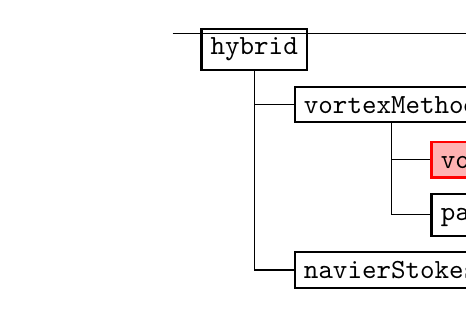
\begin{tikzpicture}[%
  grow via three points={one child at (0.5,-0.7) and
  two children at (0.5,-0.7) and (0.5,-1.4)},
  edge from parent path={(\tikzparentnode.south) |- (\tikzchildnode.west)}]
  \node {\texttt{hybrid}}
    child { node {\texttt{vortexMethod}}
    	child {node [selected] {\texttt{vortexBlobs}}}
    	child {node {\texttt{panels}}}  	
    }
    child [missing] {}				
    child [missing] {}				
    child { node {\texttt{navierStokes}}};
    %child { node [selected] {tex}
    %  child { node {generic}}
    %  child { node [optional] {latex}}
    %  child { node {plain}}
    %}
    %child [missing] {}
    %child { node {texdoc}};
\end{tikzpicture}
\end{figure}

\subsection*{Class structure:}
\begin{figure}[h]
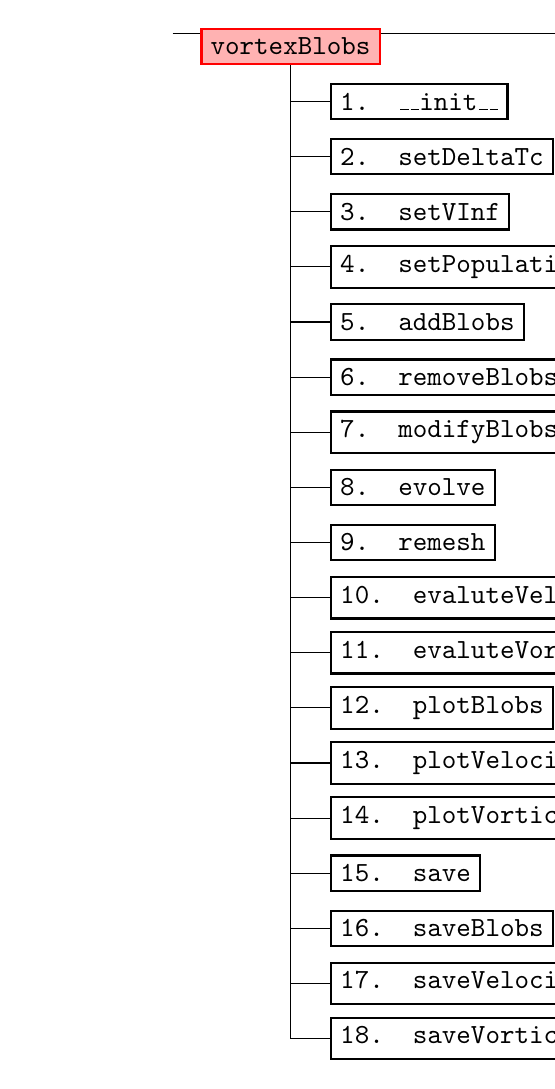
\begin{tikzpicture}[%
  grow via three points={one child at (0.5,-0.7) and
  two children at (0.5,-0.7) and (0.5,-1.4)},
  edge from parent path={(\tikzparentnode.south) |- (\tikzchildnode.west)}]
  \node [selected] {\texttt{vortexBlobs}}
    child { node {\texttt{1. \_\_init\_\_}}}
    child { node {\texttt{2. setDeltaTc}}}
    child { node {\texttt{3. setVInf}}}    
    child { node {\texttt{4. setPopulationControl}}}
    child { node {\texttt{5. addBlobs}}}
    child { node {\texttt{6. removeBlobs}}}    
    child { node {\texttt{7. modifyBlobs}}}    
    child { node {\texttt{8. evolve}}}    
    child { node {\texttt{9. remesh}}}    
    child { node {\texttt{10. evaluteVelocity}}}                    
    child { node {\texttt{11. evaluteVorticity}}}                        
    child { node {\texttt{12. plotBlobs}}}                        
    child { node {\texttt{13. plotVelocity}}}                        
    child { node {\texttt{14. plotVorticity}}}                            
    child { node {\texttt{15. save}}}                        
    child { node {\texttt{16. saveBlobs}}}                                        
    child { node {\texttt{17. saveVelocity}}}                                            
    child { node {\texttt{18. saveVorticity}}};
%    child { node [optional] {19. \texttt{\_generateBlobs}}}
%    child { node [optional] {20. \texttt{\_populationControl}}};        
        %child { node [selected] {tex}
    %  child { node {generic}}
    %  child { node [optional] {latex}}
    %  child { node {plain}}
    %}
    %child { node {texdoc}};
\end{tikzpicture}
\end{figure}

%\subsection*{Structure:}
%\begin{table}[h]
%\begin{tabular}{rl}
%	\texttt{vortexBlobs}: &  \\ \hline
%	-- & \texttt{\_\_init\_\_} \\
%	& \\
%	-- & \texttt{set\_deltaTc} \\ 
%	-- & \texttt{set\_popControlParameters} \\ 
%	-- & \texttt{addBlobs} \\ 
%	-- & \texttt{removeBlobs} \\ 
%	-- & \texttt{modifyBlobs} \\ 
%	-- & \texttt{evolve} \\ 
%	-- & \texttt{remesh} \\ 
%	-- & \texttt{evaluteVelocity} \\ 
%	-- & \texttt{evaluteVorticity} \\ 
%	-- & \texttt{plotBlobs} \\	
%	-- & \texttt{plotVelocity} \\
%	-- & \texttt{plotVorticity} \\
%	-- & \texttt{saveClass} \\ 
%	-- & \texttt{saveBlob} \\ 
%	-- & \texttt{saveVelocity} \\ 	
%	-- & \texttt{saveVorticity} \\ 
%	-- & \texttt{saveBlobPlot} \\ 
%	-- & \texttt{saveVelocityPlot} \\ 	
%	-- & \texttt{saveVorticityPlot} \\ 		
%	& \\
%	-- & \texttt{\_generateParticles} \\ 
%	-- & \texttt{\_popControl} \\
%\end{tabular}
%\end{table}

\newpage



\subsection{\texttt{\_\_init\_\_}}
	\paragraph{Description:} Initialize the \texttt{vortexBlobs} class with either the given input parameters or by a reading a \texttt{file} containing all the necessary parameters.\\
	
	\begin{tabular}{l|lp{7cm}}
		\multicolumn{2}{l}{\textbf{Input Parameters}} & \\ \hline
		\textit{File Name} & \multicolumn{2}{l}{Containing all the parameters to re-initalize the class.} \\ \cline{2-3}
		\multicolumn{3}{c}{--- or ---} \\ \cline{2-3}
		\multirow{4}{*}{\textit{Parameters}} & Vorticity Field &: \{\texttt{xBlob, yBlob, gBlob}\} or \{\texttt{wFunction, xBounds, yBounds}\}\\ \cline{2-3}
		& Blob parameters &: \texttt{overlap, h} \\ \cline{2-3}
		& Time Step parameters &: \texttt{deltaTc, nu, stepRedistribution, integrationMethod, computationMethod}\\ \cline{2-3}
		& Population control parameters &: \texttt{stepPopulationControl, gThreshold}\\ \cline{2-3}
	\end{tabular}\\
	
	\subsubsection*{Descriptions of the parameters:}
	\begin{tabular}{p{3.5cm}p{9cm}p{1cm}}
				\textit{Vorticity field} & & \textit{Default}\\ \hline
				\texttt{xBlob,yBlob} &:  the $x,y$ blob coordinates. & - \\
				\texttt{gBlob} &: the circulation $\Gamma_i$ associated to each of the vortex blobs. & - \\
				& & \\
				\multicolumn{2}{c}{\textit{--- or ---}} & \\
				& & \\
				\texttt{wExactFunction} &: the function that returns the exact value of vorticity $\omega$ at any given $x,y$ coordinates. &\\
				& 	\begin{tabular}{lp{10cm}}
						\textbf{Input parameters} &: \texttt{xEval,yEval}\\ 
						\textbf{Assigns} &: \texttt{-}\\ 			
						\textbf{Returns} &: \texttt{wEval}\\ 					
					\end{tabular} & - \\
				\texttt{xBounds, yBounds} &: the $x,y$ bounds of the domain where the particles was originally distributed. & - \\		 
	\end{tabular}\\
	\\ \\
	%	\begin{tabular}{lp{10cm}}
	%		\textbf{Input parameters} &: \texttt{xEval,yEval}\\ 
	%		\textbf{Assigns} &: \texttt{-}\\ 			
	%		\textbf{Returns} &: \texttt{vortEval}\\ 					
	%	\end{tabular}\\
	\begin{tabular}{p{3.5cm}p{9cm}p{1cm}}
				\multicolumn{2}{l}{\textit{Blob parameters}} & \textit{Default} \\ \hline				
				\texttt{overlap} &: the overlap ratio $h/\sigma$. & 1.0\\
				\texttt{h} &: the size of the cell $h$ associated to the blobs. \textit{Note:} Cells are square. & -\\
	\end{tabular}\\
	\\ \\
	\begin{tabular}{p{3.5cm}p{9cm}p{1cm}}
				\multicolumn{2}{l}{\textit{Time step parameters}} & \textit{Default}\\ \hline
				\texttt{deltaTc} &:  the size of the convective time step $\Delta t_c$. & - \\
				\texttt{nu} &: the fluid kinematic viscosity $\nu$, used to calculate the diffusion coefficient $c^2$ and diffusion time step size $\Delta T_d$.& - \\
				\texttt{stepRedistribution} &: the redistribution step frequency. & 1 \\
				\texttt{integrationMethod} &: the time integration method (\texttt{FE}: Forward euler , \texttt{RK4}: $4^{th}$ order Runge-Kutta). & RK4 \\
				\texttt{computationMethod} &: the calculation method to evolve the blobs, (\texttt{Direct}: Direct Method, \texttt{FMM}: Fast-Multipole Method) using (\texttt{CPU}, \texttt{GPU}). & \{FMM, GPU\}.\\
	\end{tabular}\\ 
    \\ \\ 
	\begin{tabular}{p{3.5cm}p{9cm}p{1cm}}
				\multicolumn{2}{l}{\textit{Population control parameters}} & \textit{Default} \\ \hline
				\texttt{stepPopulationControl} &: population control step frequency & 1.\\
				\texttt{gThreshold} &: the tuple with minimum \textbf{and} maximum value of the circulation $\Gamma_{min}$. & - \\
	\end{tabular}\\ 
    \\ \\  
	\begin{tabular}{p{3.5cm}p{9cm}p{1cm}}
				\multicolumn{2}{l}{\textit{Free stream velocity}} & \textit{Default}\\ \hline
				\texttt{vInf} &: The free-stream velocity function, returning the velocity action on the vortex blobs. & -\\		
				&		\begin{tabular}{lp{10cm}}
							\textbf{Input parameters} &: \texttt{t}\\ 
							\textbf{Assigns} &: \texttt{-}\\ 			
							\textbf{Returns} &: \texttt{vx,vy}\\ 					
						\end{tabular} & - \\
				
	\end{tabular}\\


\subsection{\texttt{setDeltaTc}}
	\paragraph{Description:} Function change the convective time step size $\Delta t_c$.\\
	
	 \begin{tabular}{p{3.5cm}p{10cm}p{1cm}}
				\multicolumn{2}{l}{\textit{Parameters}} & \textit{Default} \\ \hline
		   		\texttt{deltaTc} &: the new convection time step size $\Delta t_c$. & - \\
		\end{tabular} \vspace{5 mm}\\
	\\		
	\begin{tabular}{lp{10cm}}
		\textbf{Input parameters} &: \texttt{deltaTcNew}\\
		\textbf{Assigns} &:  \texttt{deltaTc}\\
		\textbf{Returns} &: \texttt{-}\\
	\end{tabular}

\subsection{\texttt{setPopulationControl}}
	\paragraph{Description:} function to modify the population control parameters.\\
	
	 \begin{tabular}{lp{10cm}}
				\textit{Parameters} & \\ \hline
		   		\texttt{gThresholdNew} &: the minimum and maximum circulation of the blobs, $\Gamma_{min}$\\
		   		\texttt{stepPopulationControlNew} &: the step number (frequency) of the population control.\\
		\end{tabular} \vspace{5 mm}\\
	\\		
	\begin{tabular}{lp{10cm}}
		\textbf{Input parameters} &: \texttt{gThresholdNew, stepPopulationControlNew}\\
		\textbf{Assigns} &:  \texttt{gThreshold, stepPopulationControl}\\
		\textbf{Returns} &: \texttt{-}\\
	\end{tabular}

		
\subsection{\texttt{addBlobs}}
	\paragraph{Description:} adds vortex particles by appending to the current set of particles.\\
	
	 \begin{tabular}{lp{10cm}}
				\textit{Parameters} & \\ \hline
		   		\texttt{xBlobNew,yBlobNew,gBlobNew} &: the coordinates and the strength of the new set of particles.\\
		\end{tabular} \vspace{5 mm}\\
	\\		
	\begin{tabular}{lp{10cm}}
		\textbf{Input parameters} &: \texttt{xBlobNew,yBlobNew,gBlobNew}\\
		\textbf{Assigns} &: \texttt{xBlob,yBlob,gBlob}\\
		\textbf{Returns} &: \texttt{-}\\
	\end{tabular}


\subsection{\texttt{removeBlobs}}
	\paragraph{Description:} removes vortex particles from the current set of particles. Using, the particle index, the associated $x,y$ and $\Gamma_i$ will be removed.\\
	
	 \begin{tabular}{lp{10cm}}
				\textit{Parameters} & \\ \hline
		   		\texttt{iBlob} &: the list of blob indices that is to be removed.\\
		\end{tabular} \vspace{5 mm}\\
	\\		
	\begin{tabular}{lp{10cm}}
		\textbf{Input parameters} &: \texttt{iBlob}\\
		\textbf{Assigns} &: \texttt{xBlob,yBlob,gBlob}\\
		\textbf{Returns} &: \texttt{-}\\
	\end{tabular}
	
	
\subsection{\texttt{modifyBlobs}}
	\paragraph{Description:} Replace the vortex particle strengths with the new strength.\\
	
	 \begin{tabular}{lp{10cm}}
				\textit{Parameters} & \\ \hline
		   		\texttt{iBlob} &: the list of blob indices that is to be modified.\\
		   		\texttt{gBlobNew} &: the new strength of the blobs.\\		   		
		\end{tabular} \vspace{5 mm}\\
	\\		
	\begin{tabular}{lp{10cm}}
		\textbf{Input parameters} &: \texttt{iBlob,gBlobNew}\\
		\textbf{Assigns} &: \texttt{gBlob}\\
		\textbf{Returns} &: \texttt{-}\\
	\end{tabular}	

\subsection{\texttt{evolve}}
	\paragraph{Description:} Evolves the vortex blobs according to the \texttt{\_\_init\_\_} definition. The \texttt{evolve} function, knows when (has a counter) to redistribute and perform population control. Depending on the diffusion time step $\Delta t_d$, the evolve function will also perform the diffusion process (modified interpolation).\\
	
	 \begin{tabular}{lp{10cm}}
				\textit{Parameters} & \\ \hline
		   		\texttt{xBlobNew,yBlobNew,gBlobNew} &: the new set of particle after the evolution process.\\
		\end{tabular} \vspace{5 mm}\\
	\\		
	\begin{tabular}{lp{10cm}}
		\textbf{Input parameters} &: \texttt{-}\\
		\textbf{Assigns} &: \texttt{xBlob,yBlob,gBlob}\\	
		\textbf{Returns} &: \texttt{-}\\
	\end{tabular}			


\subsection{\texttt{remesh}}
	\paragraph{Description:}  Function to remesh the particles on to the remeshing grid. When $c=0$, the remeshing will be done without diffusion. If $c>0$, the modified interpolation will perform the diffusion.
	\\
	\\		
	\begin{tabular}{lp{10cm}}
		\textbf{Input parameters} &: \texttt{c}\\ 
		\textbf{Assigns} &: \texttt{xBlob,yBlob,wBlob}\\ 			
		\textbf{Returns} &: \texttt{-}\\ 					
	\end{tabular}


\subsection{\texttt{evaluateVelocity}}
	\paragraph{Description:} Function to evaluate the total induced velocity due to the blobs, and the external velocity at a given target locations.\\
	
	    \begin{tabular}{lp{10cm}}
			\textit{Parameters} & \\ \hline
			 \texttt{xTarget,yTarget} &: the $x,y$ coordinate of the target location, where the total velocity is to be evaluated.\\
			\texttt{vxTarget,vyTarget} &: the $x,y$ induced velocity at the target points in global coordinate system.\\
		\end{tabular} \vspace{5 mm}
	\\		
	\begin{tabular}{lp{10cm}}
		\textbf{Input parameters} &: \texttt{xTarget,yTarget}\\ 
		\textbf{Assigns} &: \texttt{-}\\ 			
		\textbf{Returns} &: \texttt{vxTarget,vyTarget}\\ 					
	\end{tabular}	

\subsection{\texttt{evaluateVorticity}}
	\paragraph{Description:} Function to evaluate the total induced vorticity due to the blobs, and the external velocity at a given target coordinates.\\
	
	    \begin{tabular}{lp{10cm}}
			\textit{Parameters} & \\ \hline
			 \texttt{xTarget,yTarget} &: the $x,y$ coordinate of the target location, where the total velocity is to be evaluated.\\
			\texttt{wTarget} &: the $x,y$ induced vorticity at the target points in global coordinate system.\\
		\end{tabular} \vspace{5 mm}
	\\		
	\begin{tabular}{lp{10cm}}
		\textbf{Input parameters} &: \texttt{xTarget,yTarget}\\ 
		\textbf{Assigns} &: \texttt{-}\\ 			
		\textbf{Returns} &: \texttt{wTarget}\\ 					
	\end{tabular}


		
\subsection{plots \ldots}
	\paragraph{Description:} functions to plot and/or save all the results in a given region. The data should be store for scientific visualization (paraview format)\\
	
		\begin{tabular}{lp{10cm}}
			\textit{Plot variables:} & \\ \hline
			\texttt{plotBlob} &: plot the coordinates and the circulation of the blobs.\\
			\texttt{plotVelocity} &: plot the velocity field.\\ 
			\texttt{plotVorticity} &: plot the vorticity field.\\ 
		\end{tabular} \vspace{5 mm}
		
		\begin{tabular}{lp{10cm}}
			\textit{Parameters:} & \\ \hline
			\texttt{xBounds,yBounds} &: $x,y$ bounds of the grid, where the data is to be evaluated.\\ 
			\texttt{nGrid} &: $x,y$ number of grid points.\\
		\end{tabular} \vspace{5 mm}\\
	\\
	\begin{tabular}{lp{10cm}}
		\textbf{Input parameters} &: \texttt{xBounds,yBounds,nGrid}\\
		\textbf{Assigns} &: \texttt{-}\\ 			
		\textbf{Returns} &: \texttt{figureHandle} or \texttt{.pvd}\\ 					
	\end{tabular}	

\subsection{save data \ldots}
	\paragraph{Description:} functions to save the data. The data file will be in compressed, binary format to store efficiently.\\

		\begin{tabular}{lp{10cm}}
			\textit{Save variables:} & \\ \hline
			\texttt{save} &: all the data of the \texttt{vortexBlob} class is saved. This can be used later to restart the problem, i.e the parameter to init the problem.\\
			\texttt{saveBlobs} &: the function to save the blob data at the current time instant. List of numpy array.\\ 			
			\texttt{saveVelocity} &: save the velocity field of a given region or a given set of points.\\ 
			\texttt{saveVorticity} &: save the vorticity field of the given region or the given set of points.\\ 
		\end{tabular} \vspace{5 mm}
	
		\begin{tabular}{lp{10cm}}
			\textit{Parameters:} & \\ \hline
			\texttt{xBounds,yBounds} &: $x,y$ bounds of the grid, where the data is to be evaluated and saved.\\ 
			\texttt{nGrid} &: $x,y$ number of grid points.\\
			\texttt{xEval,yEval} &: $x,y$ coordinates of the location where the data is to be evaluated and saved.\\ 
		\end{tabular} \vspace{5 mm}\\
	\\
	\begin{tabular}{lp{10cm}}
		\textbf{Input parameters} &: \texttt{xBounds,yBounds,hGrid} or \texttt{xEval,yEval}\\ 
		\textbf{Assigns} &: \texttt{-}\\ 			
		\textbf{Returns} &: \texttt{.npz, .bin or similar}\\ 					
	\end{tabular}



%\subsection{save plots \ldots}
%	\paragraph{Description:} Function to save the plots as scientific visualization format \texttt{.pvd}.\\
%	
%		\begin{tabular}{lp{10cm}}
%			\textit{Save variables:} & \\ \hline
%			\texttt{saveBlobPlot} &: save the particle position and strengths as glyphs.\\
%			\texttt{saveVelocityPlot} &: save the velocity plot of a given region.\\ 
%			\texttt{saveVorticityPlot} &: save the vorticity of a given region.\\ 
%		\end{tabular} \vspace{5 mm}
%		
%		\begin{tabular}{lp{10cm}}
%			\textit{Parameters:} & \\ \hline
%			\texttt{xBounds,yBounds} &: $x,y$ bounds of the grid, where the data is to be evaluated and saved.\\ 
%			\texttt{hGrid} &: $x,y$ spacing of the evaluation grid.\\
%		\end{tabular} \vspace{5 mm}\\
%	\\
%	\begin{tabular}{lp{10cm}}
%		\textbf{Input parameters} &: \texttt{xBounds,yBounds,hGrid}\\
%		\textbf{Assigns} &: \texttt{-}\\ 			
%		\textbf{Returns} &: \texttt{.pvd}\\ 					
%	\end{tabular}
	


%\subsection{\texttt{\_generateParticles}}
%	\paragraph{Description:} \textit{Internal} function to generate/initialize the particles.\\
%	\\
%	\\
%		\begin{tabular}{lp{10cm}}
%			\textbf{Input parameters} &: \texttt{wExactFunction, xBounds, yBounds}\\ 
%			\textbf{Assigns} &: \texttt{xBlob,yBlob,wBlob}\\ 			
%			\textbf{Returns} &: \texttt{-}\\ 					
%		\end{tabular}	
%
%
%\subsection{\texttt{\_popControl}}
%	\paragraph{Description:} \textit{Internal} function to perform population control on the current set of particles.\\
%	\\
%	\\	
%		\begin{tabular}{lp{10cm}}
%			\textbf{Input parameters} &: \texttt{-}\\ 
%			\textbf{Assigns} &: \texttt{xBlob,yBlob,wBlob}\\ 			
%			\textbf{Returns} &: \texttt{-}\\ 					
%		\end{tabular}	
%\section{\texttt{vortexBlobs}}
The main structure of the \texttt{vortexBlobs} class. This class contains all the function related to the calculation of the vortex blobs.
\begin{figure}[h]
\centering
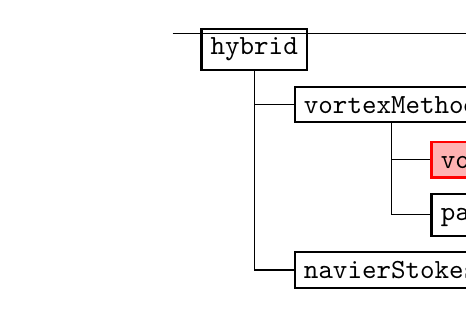
\begin{tikzpicture}[%
  grow via three points={one child at (0.5,-0.7) and
  two children at (0.5,-0.7) and (0.5,-1.4)},
  edge from parent path={(\tikzparentnode.south) |- (\tikzchildnode.west)}]
  \node {\texttt{hybrid}}
    child { node {\texttt{vortexMethod}}
    	child {node [selected] {\texttt{vortexBlobs}}}
    	child {node {\texttt{panels}}}  	
    }
    child [missing] {}				
    child [missing] {}				
    child { node {\texttt{navierStokes}}};
    %child { node [selected] {tex}
    %  child { node {generic}}
    %  child { node [optional] {latex}}
    %  child { node {plain}}
    %}
    %child [missing] {}
    %child { node {texdoc}};
\end{tikzpicture}
\end{figure}

\subsection*{Class structure:}
\begin{figure}[h]
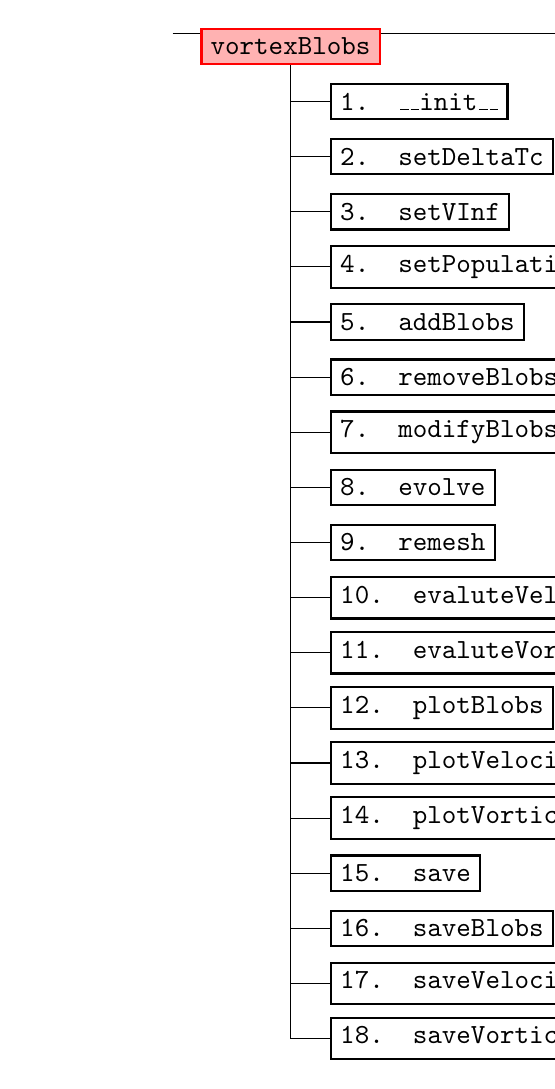
\begin{tikzpicture}[%
  grow via three points={one child at (0.5,-0.7) and
  two children at (0.5,-0.7) and (0.5,-1.4)},
  edge from parent path={(\tikzparentnode.south) |- (\tikzchildnode.west)}]
  \node [selected] {\texttt{vortexBlobs}}
    child { node {\texttt{1. \_\_init\_\_}}}
    child { node {\texttt{2. setDeltaTc}}}
    child { node {\texttt{3. setVInf}}}    
    child { node {\texttt{4. setPopulationControl}}}
    child { node {\texttt{5. addBlobs}}}
    child { node {\texttt{6. removeBlobs}}}    
    child { node {\texttt{7. modifyBlobs}}}    
    child { node {\texttt{8. evolve}}}    
    child { node {\texttt{9. remesh}}}    
    child { node {\texttt{10. evaluteVelocity}}}                    
    child { node {\texttt{11. evaluteVorticity}}}                        
    child { node {\texttt{12. plotBlobs}}}                        
    child { node {\texttt{13. plotVelocity}}}                        
    child { node {\texttt{14. plotVorticity}}}                            
    child { node {\texttt{15. save}}}                        
    child { node {\texttt{16. saveBlobs}}}                                        
    child { node {\texttt{17. saveVelocity}}}                                            
    child { node {\texttt{18. saveVorticity}}};
%    child { node [optional] {19. \texttt{\_generateBlobs}}}
%    child { node [optional] {20. \texttt{\_populationControl}}};        
        %child { node [selected] {tex}
    %  child { node {generic}}
    %  child { node [optional] {latex}}
    %  child { node {plain}}
    %}
    %child { node {texdoc}};
\end{tikzpicture}
\end{figure}

%\subsection*{Structure:}
%\begin{table}[h]
%\begin{tabular}{rl}
%	\texttt{vortexBlobs}: &  \\ \hline
%	-- & \texttt{\_\_init\_\_} \\
%	& \\
%	-- & \texttt{set\_deltaTc} \\ 
%	-- & \texttt{set\_popControlParameters} \\ 
%	-- & \texttt{addBlobs} \\ 
%	-- & \texttt{removeBlobs} \\ 
%	-- & \texttt{modifyBlobs} \\ 
%	-- & \texttt{evolve} \\ 
%	-- & \texttt{remesh} \\ 
%	-- & \texttt{evaluteVelocity} \\ 
%	-- & \texttt{evaluteVorticity} \\ 
%	-- & \texttt{plotBlobs} \\	
%	-- & \texttt{plotVelocity} \\
%	-- & \texttt{plotVorticity} \\
%	-- & \texttt{saveClass} \\ 
%	-- & \texttt{saveBlob} \\ 
%	-- & \texttt{saveVelocity} \\ 	
%	-- & \texttt{saveVorticity} \\ 
%	-- & \texttt{saveBlobPlot} \\ 
%	-- & \texttt{saveVelocityPlot} \\ 	
%	-- & \texttt{saveVorticityPlot} \\ 		
%	& \\
%	-- & \texttt{\_generateParticles} \\ 
%	-- & \texttt{\_popControl} \\
%\end{tabular}
%\end{table}

\newpage



\subsection{\texttt{\_\_init\_\_}}
	\paragraph{Description:} Initialize the \texttt{vortexBlobs} class with either the given input parameters or by a reading a \texttt{file} containing all the necessary parameters.\\
	
	\begin{tabular}{l|lp{7cm}}
		\multicolumn{2}{l}{\textbf{Input Parameters}} & \\ \hline
		\textit{File Name} & \multicolumn{2}{l}{Containing all the parameters to re-initalize the class.} \\ \cline{2-3}
		\multicolumn{3}{c}{--- or ---} \\ \cline{2-3}
		\multirow{4}{*}{\textit{Parameters}} & Vorticity Field &: \{\texttt{xBlob, yBlob, gBlob}\} or \{\texttt{wFunction, xBounds, yBounds}\}\\ \cline{2-3}
		& Blob parameters &: \texttt{overlap, h} \\ \cline{2-3}
		& Time Step parameters &: \texttt{deltaTc, nu, stepRedistribution, integrationMethod, computationMethod}\\ \cline{2-3}
		& Population control parameters &: \texttt{stepPopulationControl, gThreshold}\\ \cline{2-3}
	\end{tabular}\\
	
	\subsubsection*{Descriptions of the parameters:}
	\begin{tabular}{p{3.5cm}p{9cm}p{1cm}}
				\textit{Vorticity field} & & \textit{Default}\\ \hline
				\texttt{xBlob,yBlob} &:  the $x,y$ blob coordinates. & - \\
				\texttt{gBlob} &: the circulation $\Gamma_i$ associated to each of the vortex blobs. & - \\
				& & \\
				\multicolumn{2}{c}{\textit{--- or ---}} & \\
				& & \\
				\texttt{wExactFunction} &: the function that returns the exact value of vorticity $\omega$ at any given $x,y$ coordinates. &\\
				& 	\begin{tabular}{lp{10cm}}
						\textbf{Input parameters} &: \texttt{xEval,yEval}\\ 
						\textbf{Assigns} &: \texttt{-}\\ 			
						\textbf{Returns} &: \texttt{wEval}\\ 					
					\end{tabular} & - \\
				\texttt{xBounds, yBounds} &: the $x,y$ bounds of the domain where the particles was originally distributed. & - \\		 
	\end{tabular}\\
	\\ \\
	%	\begin{tabular}{lp{10cm}}
	%		\textbf{Input parameters} &: \texttt{xEval,yEval}\\ 
	%		\textbf{Assigns} &: \texttt{-}\\ 			
	%		\textbf{Returns} &: \texttt{vortEval}\\ 					
	%	\end{tabular}\\
	\begin{tabular}{p{3.5cm}p{9cm}p{1cm}}
				\multicolumn{2}{l}{\textit{Blob parameters}} & \textit{Default} \\ \hline				
				\texttt{overlap} &: the overlap ratio $h/\sigma$. & 1.0\\
				\texttt{h} &: the size of the cell $h$ associated to the blobs. \textit{Note:} Cells are square. & -\\
	\end{tabular}\\
	\\ \\
	\begin{tabular}{p{3.5cm}p{9cm}p{1cm}}
				\multicolumn{2}{l}{\textit{Time step parameters}} & \textit{Default}\\ \hline
				\texttt{deltaTc} &:  the size of the convective time step $\Delta t_c$. & - \\
				\texttt{nu} &: the fluid kinematic viscosity $\nu$, used to calculate the diffusion coefficient $c^2$ and diffusion time step size $\Delta T_d$.& - \\
				\texttt{stepRedistribution} &: the redistribution step frequency. & 1 \\
				\texttt{integrationMethod} &: the time integration method (\texttt{FE}: Forward euler , \texttt{RK4}: $4^{th}$ order Runge-Kutta). & RK4 \\
				\texttt{computationMethod} &: the calculation method to evolve the blobs, (\texttt{Direct}: Direct Method, \texttt{FMM}: Fast-Multipole Method) using (\texttt{CPU}, \texttt{GPU}). & \{FMM, GPU\}.\\
	\end{tabular}\\ 
    \\ \\ 
	\begin{tabular}{p{3.5cm}p{9cm}p{1cm}}
				\multicolumn{2}{l}{\textit{Population control parameters}} & \textit{Default} \\ \hline
				\texttt{stepPopulationControl} &: population control step frequency & 1.\\
				\texttt{gThreshold} &: the tuple with minimum \textbf{and} maximum value of the circulation $\Gamma_{min}$. & - \\
	\end{tabular}\\ 
    \\ \\  
	\begin{tabular}{p{3.5cm}p{9cm}p{1cm}}
				\multicolumn{2}{l}{\textit{Free stream velocity}} & \textit{Default}\\ \hline
				\texttt{vInf} &: The free-stream velocity function, returning the velocity action on the vortex blobs. & -\\		
				&		\begin{tabular}{lp{10cm}}
							\textbf{Input parameters} &: \texttt{t}\\ 
							\textbf{Assigns} &: \texttt{-}\\ 			
							\textbf{Returns} &: \texttt{vx,vy}\\ 					
						\end{tabular} & - \\
				
	\end{tabular}\\


\subsection{\texttt{setDeltaTc}}
	\paragraph{Description:} Function change the convective time step size $\Delta t_c$.\\
	
	 \begin{tabular}{p{3.5cm}p{10cm}p{1cm}}
				\multicolumn{2}{l}{\textit{Parameters}} & \textit{Default} \\ \hline
		   		\texttt{deltaTc} &: the new convection time step size $\Delta t_c$. & - \\
		\end{tabular} \vspace{5 mm}\\
	\\		
	\begin{tabular}{lp{10cm}}
		\textbf{Input parameters} &: \texttt{deltaTcNew}\\
		\textbf{Assigns} &:  \texttt{deltaTc}\\
		\textbf{Returns} &: \texttt{-}\\
	\end{tabular}

\subsection{\texttt{setPopulationControl}}
	\paragraph{Description:} function to modify the population control parameters.\\
	
	 \begin{tabular}{lp{10cm}}
				\textit{Parameters} & \\ \hline
		   		\texttt{gThresholdNew} &: the minimum and maximum circulation of the blobs, $\Gamma_{min}$\\
		   		\texttt{stepPopulationControlNew} &: the step number (frequency) of the population control.\\
		\end{tabular} \vspace{5 mm}\\
	\\		
	\begin{tabular}{lp{10cm}}
		\textbf{Input parameters} &: \texttt{gThresholdNew, stepPopulationControlNew}\\
		\textbf{Assigns} &:  \texttt{gThreshold, stepPopulationControl}\\
		\textbf{Returns} &: \texttt{-}\\
	\end{tabular}

		
\subsection{\texttt{addBlobs}}
	\paragraph{Description:} adds vortex particles by appending to the current set of particles.\\
	
	 \begin{tabular}{lp{10cm}}
				\textit{Parameters} & \\ \hline
		   		\texttt{xBlobNew,yBlobNew,gBlobNew} &: the coordinates and the strength of the new set of particles.\\
		\end{tabular} \vspace{5 mm}\\
	\\		
	\begin{tabular}{lp{10cm}}
		\textbf{Input parameters} &: \texttt{xBlobNew,yBlobNew,gBlobNew}\\
		\textbf{Assigns} &: \texttt{xBlob,yBlob,gBlob}\\
		\textbf{Returns} &: \texttt{-}\\
	\end{tabular}


\subsection{\texttt{removeBlobs}}
	\paragraph{Description:} removes vortex particles from the current set of particles. Using, the particle index, the associated $x,y$ and $\Gamma_i$ will be removed.\\
	
	 \begin{tabular}{lp{10cm}}
				\textit{Parameters} & \\ \hline
		   		\texttt{iBlob} &: the list of blob indices that is to be removed.\\
		\end{tabular} \vspace{5 mm}\\
	\\		
	\begin{tabular}{lp{10cm}}
		\textbf{Input parameters} &: \texttt{iBlob}\\
		\textbf{Assigns} &: \texttt{xBlob,yBlob,gBlob}\\
		\textbf{Returns} &: \texttt{-}\\
	\end{tabular}
	
	
\subsection{\texttt{modifyBlobs}}
	\paragraph{Description:} Replace the vortex particle strengths with the new strength.\\
	
	 \begin{tabular}{lp{10cm}}
				\textit{Parameters} & \\ \hline
		   		\texttt{iBlob} &: the list of blob indices that is to be modified.\\
		   		\texttt{gBlobNew} &: the new strength of the blobs.\\		   		
		\end{tabular} \vspace{5 mm}\\
	\\		
	\begin{tabular}{lp{10cm}}
		\textbf{Input parameters} &: \texttt{iBlob,gBlobNew}\\
		\textbf{Assigns} &: \texttt{gBlob}\\
		\textbf{Returns} &: \texttt{-}\\
	\end{tabular}	

\subsection{\texttt{evolve}}
	\paragraph{Description:} Evolves the vortex blobs according to the \texttt{\_\_init\_\_} definition. The \texttt{evolve} function, knows when (has a counter) to redistribute and perform population control. Depending on the diffusion time step $\Delta t_d$, the evolve function will also perform the diffusion process (modified interpolation).\\
	
	 \begin{tabular}{lp{10cm}}
				\textit{Parameters} & \\ \hline
		   		\texttt{xBlobNew,yBlobNew,gBlobNew} &: the new set of particle after the evolution process.\\
		\end{tabular} \vspace{5 mm}\\
	\\		
	\begin{tabular}{lp{10cm}}
		\textbf{Input parameters} &: \texttt{-}\\
		\textbf{Assigns} &: \texttt{xBlob,yBlob,gBlob}\\	
		\textbf{Returns} &: \texttt{-}\\
	\end{tabular}			


\subsection{\texttt{remesh}}
	\paragraph{Description:}  Function to remesh the particles on to the remeshing grid. When $c=0$, the remeshing will be done without diffusion. If $c>0$, the modified interpolation will perform the diffusion.
	\\
	\\		
	\begin{tabular}{lp{10cm}}
		\textbf{Input parameters} &: \texttt{c}\\ 
		\textbf{Assigns} &: \texttt{xBlob,yBlob,wBlob}\\ 			
		\textbf{Returns} &: \texttt{-}\\ 					
	\end{tabular}


\subsection{\texttt{evaluateVelocity}}
	\paragraph{Description:} Function to evaluate the total induced velocity due to the blobs, and the external velocity at a given target locations.\\
	
	    \begin{tabular}{lp{10cm}}
			\textit{Parameters} & \\ \hline
			 \texttt{xTarget,yTarget} &: the $x,y$ coordinate of the target location, where the total velocity is to be evaluated.\\
			\texttt{vxTarget,vyTarget} &: the $x,y$ induced velocity at the target points in global coordinate system.\\
		\end{tabular} \vspace{5 mm}
	\\		
	\begin{tabular}{lp{10cm}}
		\textbf{Input parameters} &: \texttt{xTarget,yTarget}\\ 
		\textbf{Assigns} &: \texttt{-}\\ 			
		\textbf{Returns} &: \texttt{vxTarget,vyTarget}\\ 					
	\end{tabular}	

\subsection{\texttt{evaluateVorticity}}
	\paragraph{Description:} Function to evaluate the total induced vorticity due to the blobs, and the external velocity at a given target coordinates.\\
	
	    \begin{tabular}{lp{10cm}}
			\textit{Parameters} & \\ \hline
			 \texttt{xTarget,yTarget} &: the $x,y$ coordinate of the target location, where the total velocity is to be evaluated.\\
			\texttt{wTarget} &: the $x,y$ induced vorticity at the target points in global coordinate system.\\
		\end{tabular} \vspace{5 mm}
	\\		
	\begin{tabular}{lp{10cm}}
		\textbf{Input parameters} &: \texttt{xTarget,yTarget}\\ 
		\textbf{Assigns} &: \texttt{-}\\ 			
		\textbf{Returns} &: \texttt{wTarget}\\ 					
	\end{tabular}


		
\subsection{plots \ldots}
	\paragraph{Description:} functions to plot and/or save all the results in a given region. The data should be store for scientific visualization (paraview format)\\
	
		\begin{tabular}{lp{10cm}}
			\textit{Plot variables:} & \\ \hline
			\texttt{plotBlob} &: plot the coordinates and the circulation of the blobs.\\
			\texttt{plotVelocity} &: plot the velocity field.\\ 
			\texttt{plotVorticity} &: plot the vorticity field.\\ 
		\end{tabular} \vspace{5 mm}
		
		\begin{tabular}{lp{10cm}}
			\textit{Parameters:} & \\ \hline
			\texttt{xBounds,yBounds} &: $x,y$ bounds of the grid, where the data is to be evaluated.\\ 
			\texttt{nGrid} &: $x,y$ number of grid points.\\
		\end{tabular} \vspace{5 mm}\\
	\\
	\begin{tabular}{lp{10cm}}
		\textbf{Input parameters} &: \texttt{xBounds,yBounds,nGrid}\\
		\textbf{Assigns} &: \texttt{-}\\ 			
		\textbf{Returns} &: \texttt{figureHandle} or \texttt{.pvd}\\ 					
	\end{tabular}	

\subsection{save data \ldots}
	\paragraph{Description:} functions to save the data. The data file will be in compressed, binary format to store efficiently.\\

		\begin{tabular}{lp{10cm}}
			\textit{Save variables:} & \\ \hline
			\texttt{save} &: all the data of the \texttt{vortexBlob} class is saved. This can be used later to restart the problem, i.e the parameter to init the problem.\\
			\texttt{saveBlobs} &: the function to save the blob data at the current time instant. List of numpy array.\\ 			
			\texttt{saveVelocity} &: save the velocity field of a given region or a given set of points.\\ 
			\texttt{saveVorticity} &: save the vorticity field of the given region or the given set of points.\\ 
		\end{tabular} \vspace{5 mm}
	
		\begin{tabular}{lp{10cm}}
			\textit{Parameters:} & \\ \hline
			\texttt{xBounds,yBounds} &: $x,y$ bounds of the grid, where the data is to be evaluated and saved.\\ 
			\texttt{nGrid} &: $x,y$ number of grid points.\\
			\texttt{xEval,yEval} &: $x,y$ coordinates of the location where the data is to be evaluated and saved.\\ 
		\end{tabular} \vspace{5 mm}\\
	\\
	\begin{tabular}{lp{10cm}}
		\textbf{Input parameters} &: \texttt{xBounds,yBounds,hGrid} or \texttt{xEval,yEval}\\ 
		\textbf{Assigns} &: \texttt{-}\\ 			
		\textbf{Returns} &: \texttt{.npz, .bin or similar}\\ 					
	\end{tabular}



%\subsection{save plots \ldots}
%	\paragraph{Description:} Function to save the plots as scientific visualization format \texttt{.pvd}.\\
%	
%		\begin{tabular}{lp{10cm}}
%			\textit{Save variables:} & \\ \hline
%			\texttt{saveBlobPlot} &: save the particle position and strengths as glyphs.\\
%			\texttt{saveVelocityPlot} &: save the velocity plot of a given region.\\ 
%			\texttt{saveVorticityPlot} &: save the vorticity of a given region.\\ 
%		\end{tabular} \vspace{5 mm}
%		
%		\begin{tabular}{lp{10cm}}
%			\textit{Parameters:} & \\ \hline
%			\texttt{xBounds,yBounds} &: $x,y$ bounds of the grid, where the data is to be evaluated and saved.\\ 
%			\texttt{hGrid} &: $x,y$ spacing of the evaluation grid.\\
%		\end{tabular} \vspace{5 mm}\\
%	\\
%	\begin{tabular}{lp{10cm}}
%		\textbf{Input parameters} &: \texttt{xBounds,yBounds,hGrid}\\
%		\textbf{Assigns} &: \texttt{-}\\ 			
%		\textbf{Returns} &: \texttt{.pvd}\\ 					
%	\end{tabular}
	


%\subsection{\texttt{\_generateParticles}}
%	\paragraph{Description:} \textit{Internal} function to generate/initialize the particles.\\
%	\\
%	\\
%		\begin{tabular}{lp{10cm}}
%			\textbf{Input parameters} &: \texttt{wExactFunction, xBounds, yBounds}\\ 
%			\textbf{Assigns} &: \texttt{xBlob,yBlob,wBlob}\\ 			
%			\textbf{Returns} &: \texttt{-}\\ 					
%		\end{tabular}	
%
%
%\subsection{\texttt{\_popControl}}
%	\paragraph{Description:} \textit{Internal} function to perform population control on the current set of particles.\\
%	\\
%	\\	
%		\begin{tabular}{lp{10cm}}
%			\textbf{Input parameters} &: \texttt{-}\\ 
%			\textbf{Assigns} &: \texttt{xBlob,yBlob,wBlob}\\ 			
%			\textbf{Returns} &: \texttt{-}\\ 					
%		\end{tabular}	
%\section{\texttt{panels}}
The main structure of the panel method class \texttt{panels}. This class contains all the functions related to the calculation of panels.

\begin{figure}[h]
\centering
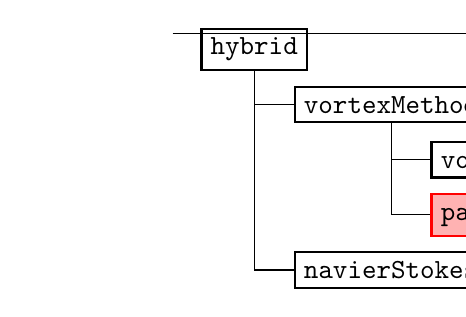
\begin{tikzpicture}[%
  grow via three points={one child at (0.5,-0.7) and
  two children at (0.5,-0.7) and (0.5,-1.4)},
  edge from parent path={(\tikzparentnode.south) |- (\tikzchildnode.west)}]
  \node {\texttt{hybrid}}
    child { node {\texttt{vortexMethod}}
    	child {node {\texttt{vortexBlobs}}}
    	child {node [selected] {\texttt{panels}}}  	
    }
    child [missing] {}				
    child [missing] {}				
    child { node {\texttt{navierStokes}}};
    %child { node [selected] {tex}
    %  child { node {generic}}
    %  child { node [optional] {latex}}
    %  child { node {plain}}
    %}
    %child [missing] {}
    %child { node {texdoc}};
\end{tikzpicture}
\end{figure}


\subsection*{Class structure:}
\begin{figure}[h]
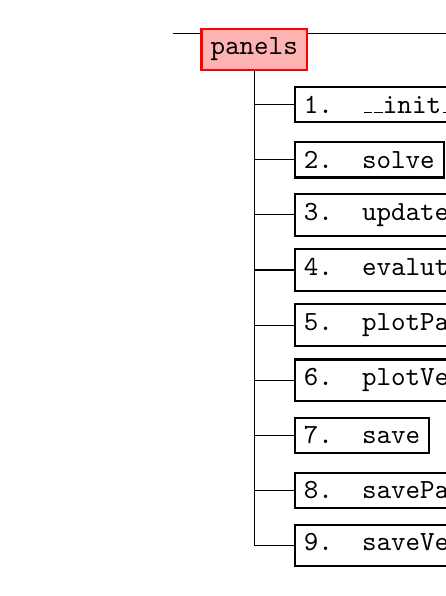
\begin{tikzpicture}[%
  grow via three points={one child at (0.5,-0.7) and
  two children at (0.5,-0.7) and (0.5,-1.4)},
  edge from parent path={(\tikzparentnode.south) |- (\tikzchildnode.west)}]
  \node [selected] {\texttt{panels}}
    child { node {\texttt{1. \_\_init\_\_}}}
    child { node {\texttt{2. solve}}}
    child { node {\texttt{3. updateBody}}}    
    child { node {\texttt{4. evaluteVelocity}}}                    
    child { node {\texttt{5. plotPanels}}}                        
    child { node {\texttt{6. plotVelocity}}}                        
    child { node {\texttt{7. save}}}                        
    child { node {\texttt{8. savePanels}}}                                        
    child { node {\texttt{9. saveVelocity}}};                                            
	%  child { node [selected] {tex}
    %  child { node {generic}}
    %  child { node [optional] {latex}}
    %  child { node {plain}}
    %}
    %child { node {texdoc}};
\end{tikzpicture}
\end{figure}

\subsection{\texttt{\_\_init\_\_}}
	\begin{tabular}{l|lp{7cm}}
		\multicolumn{2}{l}{\textbf{Input Parameters}} & \\ \hline
		\textit{File Name} & \multicolumn{2}{l}{Containing all the parameters to re-initalize the class.} \\ \hline
		\multirow{2}{*}{\textit{Parameters}} & Panel coordinates &: \{\texttt{xCP, yCP, xPanel, yPanel, cmGlobal, thetaLocal}\}\\ \cline{2-3}
		& External velocity &: \texttt{externVel} \\ \cline{2-3}
	\end{tabular}
	\paragraph{Description:} Initialize the \texttt{panels} class with the given input parameters. In the case of a multibody problem, a list of panel coordinates can be given and internally it takes care of the inter-coupling.\\
	\\
	\begin{tabular}{lp{10cm}}
				\textit{Panel coordinates} & \\ \hline
				\texttt{xCP,yCP} &:  the local $x,y$-coordinates of the panel collocation points.\\ 
				\texttt{xPanel,yPanel} &: the local coordinate of the panel edges. \textit{Note}: Should have a closed loop (end with initial point coordinates).\\ 
				\texttt{cmGlobal} &:  the position of reference points of a given panel body.\\
				\texttt{thetaLocal} &:  the rotational angles of the panel body axes w.r.t to the global $x$-axis.\\
	\end{tabular}\\ 
    \\ \\
	\begin{tabular}{lp{10cm}}
				\textit{External velocity} & \\ \hline
				\texttt{externVel} &:  Reference to an external velocity \textbf{function} acting of the panels. For the panel case, the external velocity will the induced velocity of the blobs + freestream \texttt{vortexBlob.evaluateVelocity}.\\
	\end{tabular}\\
	
		\begin{tabular}{lp{10cm}}
			\textbf{Input parameters} &: \texttt{xCP,yCP}\\ 
			\textbf{Assigns} &: \texttt{-}\\ 			
			\textbf{Returns} &: \texttt{vxCP,vyCP}\\ 					
		\end{tabular}\\

		
\subsection{\texttt{solve}}
	\paragraph{Description:} Function to solve the panel strength to satisfy no-slip condition.\\
	
		\begin{tabular}{lp{10cm}}
			\textit{Parameters} & \\ \hline
			\texttt{sPanel} &: the new strength of the panels, satisfying the no-through b.c of the body (no-slip with vortex panels.).\\
		\end{tabular} \vspace{5 mm}
		\\		
		\begin{tabular}{lp{10cm}}
			\textbf{Input parameters} &: \texttt{-}\\ 
			\textbf{Assigns} &: \texttt{sPanel}\\ 			
			\textbf{Returns} &: \texttt{-}\\ 					
		\end{tabular}		
			
		
\subsection{\texttt{updateBody}}
	\paragraph{Description:} Function to update all the panel body coordinates. This function will internally calculate the new panel coordinates \texttt{xPanel,yPanel,xCP,yCP} and rebuild the inter-induction matrix \texttt{A}.\\
	
		\begin{tabular}{lp{10cm}}
			\textit{Parameters} & \\ \hline
			\texttt{xPanel,yPanel} &: the $x,y$ panel coordinates in global.\\
			\texttt{xCP,yCP} &: the $x,y$ coordinates of the collocation point in global.\\
			\texttt{A} &: the panel self-induction matrix.
		\end{tabular} \vspace{5 mm}
		\\		
		\begin{tabular}{lp{10cm}}
			\textbf{Input parameters} &: \texttt{thetaLocals,cmGlobals}\\ 
			\textbf{Assigns} &: \texttt{A, xPanel, yPanel, xCP, yCP}\\ 			
			\textbf{Returns} &: \texttt{-}\\ 					
		\end{tabular}	

\subsection{\texttt{evaluateVelocity}}
	\paragraph{Description:} Function to evaluate the total induced velocity due to the panels and free-stream velocity (\textit{optional}).\\
	
	    \begin{tabular}{lp{10cm}}
			\textit{Parameters} & \\ \hline
			 \texttt{xTarget,yTarget} &: the $x,y$ coordinate of the target location, where the total velocity is to be evaluated.\\
			\texttt{vxTarget,vyTarget} &: the $x,y$ induced velocity of the target points in global coordinate system.\\
		\end{tabular} \vspace{5 mm}
	\\		
	\begin{tabular}{lp{10cm}}
		\textbf{Input parameters} &: \texttt{xTarget,yTarget}\\ 
		\textbf{Assigns} &: \texttt{-}\\ 			
		\textbf{Returns} &: \texttt{vxTarget,vyTarget}\\ 					
	\end{tabular}					

		
\subsection{plots \ldots}
	\paragraph{Description:} Function to plot and save (\textit{optional}) all the results in a given region or set of points.\\
	
		\begin{tabular}{lp{10cm}}
			\textit{Plot variables:} & \\ \hline
			\texttt{plotPanels} &:plot the panel coordinates at the current time instant.\\
			\texttt{plotVelocity} &: plot the velocity field.\\ 
			\texttt{plotVorticity} &: plot the vorticity field.\\ 
		\end{tabular} \vspace{5 mm}
		
		\begin{tabular}{lp{10cm}}
			\textit{Parameters:} & \\ \hline
			\texttt{xBounds,yBounds} &: $x,y$ bounds of the grid, where the data is to be evaluated and saved.\\ 
			\texttt{nGrid} &: $x,y$ number of evaluation grid points.\\ 
			\texttt{xEval,yEval} &: $x,y$ coordinates of the location where the data is to be evaluated and saved.\\ 
		\end{tabular} \vspace{5 mm}\\
	\\
	\begin{tabular}{lp{10cm}}
		\textbf{Input parameters} &: \texttt{xBounds,yBounds,hGrid} or \texttt{xEval,yEval}\\ 
		\textbf{Assigns} &: \texttt{-}\\ 			
		\textbf{Returns} &: \texttt{figureHandle} and/or \texttt{.pvd}\\ 					
	\end{tabular}	

\subsection{save data \ldots}
	\paragraph{Description:} Function to save the data in a given region or at given set of points.\\

		\begin{tabular}{lp{10cm}}
			\textit{Save variables:} & \\ \hline
			\texttt{save} &: all the data of the \texttt{panels} class, to be used to restart later.\\ 			
			\texttt{savePanels} &: the function to save the panel data at the current time instant.\\ 			
			\texttt{saveVelocity} &: save the velocity field of the given region or the given set of points.\\ 
			\texttt{saveVorticity} &: save the vorticity field of the given region or the given set of points.\\ 
		\end{tabular} \vspace{5 mm}
	
		\begin{tabular}{lp{10cm}}
			\textit{Parameters:} & \\ \hline
			\texttt{xBounds,yBounds} &: $x,y$ bounds of the grid, where the data is to be evaluated and saved.\\ 
			\texttt{nGrid} &: $x,y$ number of grid points.\\ 
			\texttt{xEval,yEval} &: $x,y$ coordinates of the location where the data is the be evaluated and saved.\\ 
		\end{tabular} \vspace{5 mm}\\
	\\
	\begin{tabular}{lp{10cm}}
		\textbf{Input parameters} &: \texttt{xBounds,yBounds,hGrid} or \texttt{xEval,yEval}\\ 
		\textbf{Assigns} &: \texttt{-}\\ 			
		\textbf{Returns} &: \texttt{.npz}\\ 					
	\end{tabular}

%
%
%\subsection{save plots \ldots}
%	\paragraph{Description:} Function to save the plots of a region or a given set of points as scientific visualization format \texttt{.pvd}.\\
%	
%		\begin{tabular}{lp{10cm}}
%			\textit{Save variables:} & \\ \hline
%			\texttt{saveVelocityPlot} &: save the velocity $\mathbf{V}$ plot.\\ 
%			\texttt{saveVorticityPlot} &: save the vorticity $\mathbf{\omega}$ plot.\\ 
%		\end{tabular} \vspace{5 mm}
%		
%		\begin{tabular}{lp{10cm}}
%			\textit{Parameters:} & \\ \hline
%			\texttt{xBounds,yBounds} &: $x,y$ bounds of the grid, where the data is to be evaluated and saved.\\ 
%			\texttt{hGrid} &: $x,y$ spacing of the evaluation grid.\\ 
%			\texttt{xEval,yEval} &: $x,y$ coordinates of the location where the data is the be evaluated and saved.\\ 
%		\end{tabular} \vspace{5 mm}\\
%	\\
%	\begin{tabular}{lp{10cm}}
%		\textbf{Input parameters} &: \texttt{xBounds,yBounds,hGrid} or \texttt{xEval,yEval} \\ 
%		\textbf{Assigns} &: \texttt{-}\\ 			
%		\textbf{Returns} &: \texttt{.pvd}\\ 					
%	\end{tabular}
%\section{\texttt{vortexMethod}}
The main structure of the \texttt{vortexBlobs} + \texttt{panels} (vortexMethod) class. This class contains all the function related to the calculations of panel with vortex blobs.

\begin{figure}[h]
\centering
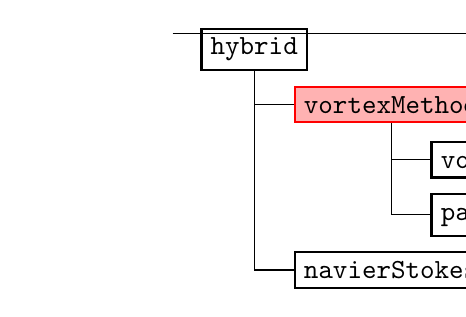
\begin{tikzpicture}[%
  grow via three points={one child at (0.5,-0.7) and
  two children at (0.5,-0.7) and (0.5,-1.4)},
  edge from parent path={(\tikzparentnode.south) |- (\tikzchildnode.west)}]
  \node {\texttt{hybrid}}
    child { node [selected] {\texttt{vortexMethod}}
    	child {node {\texttt{vortexBlobs}}}
    	child {node {\texttt{panels}}}  	
    }
    child [missing] {}				
    child [missing] {}				
    child { node {\texttt{navierStokes}}};
    %child { node [selected] {tex}
    %  child { node {generic}}
    %  child { node [optional] {latex}}
    %  child { node {plain}}
    %}
    %child [missing] {}
    %child { node {texdoc}};
\end{tikzpicture}
\end{figure}

\subsection*{Class structure:}
\begin{figure}[h]
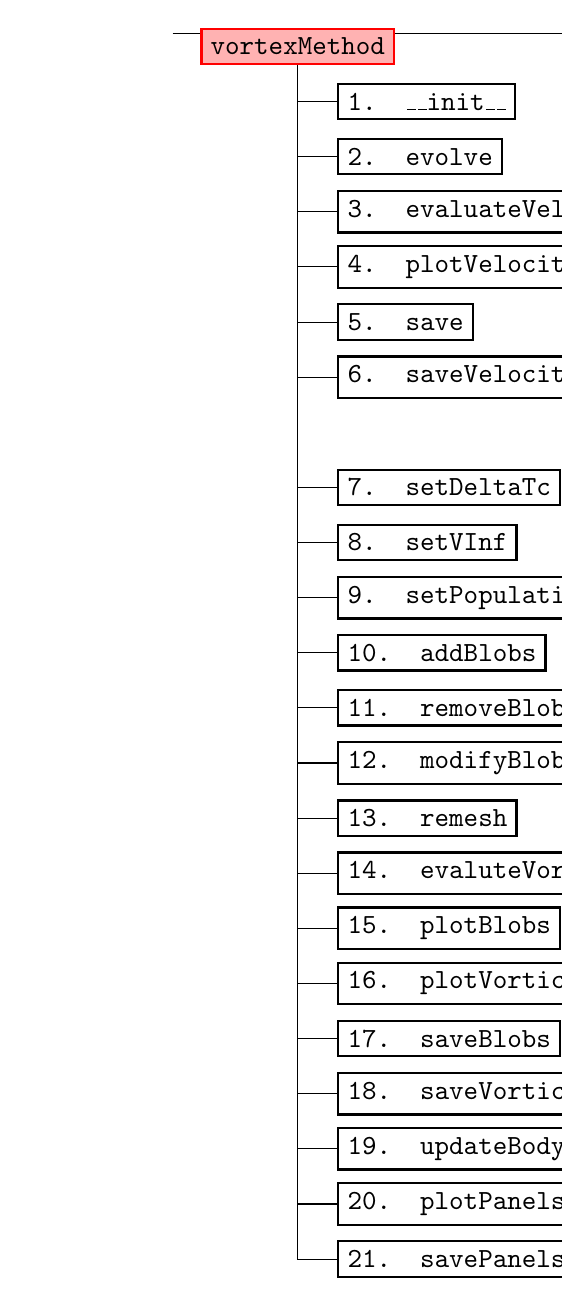
\begin{tikzpicture}[%
  grow via three points={one child at (0.5,-0.7) and
  two children at (0.5,-0.7) and (0.5,-1.4)},
  edge from parent path={(\tikzparentnode.south) |- (\tikzchildnode.west)}]
  \node [selected] {\texttt{vortexMethod}}
    child { node {\texttt{1. \_\_init\_\_}}}
    child { node {\texttt{2. evolve}}}
    child { node {\texttt{3. evaluateVelocity}}}
    child { node {\texttt{4. plotVelocity}}}                        
    child { node {\texttt{5. save}}}                        
    child { node {\texttt{6. saveVelocity}}}                                            
    child [missing] {}
    child { node {\texttt{7. setDeltaTc}}}
    child { node {\texttt{8. setVInf}}}    
    child { node {\texttt{9. setPopulationControl}}}
    child { node {\texttt{10. addBlobs}}}
    child { node {\texttt{11. removeBlobs}}}    
    child { node {\texttt{12. modifyBlobs}}}    
    child { node {\texttt{13. remesh}}}    
    child { node {\texttt{14. evaluteVorticity}}}                        
    child { node {\texttt{15. plotBlobs}}}                        
    child { node {\texttt{16. plotVorticity}}}                            
    child { node {\texttt{17. saveBlobs}}}                                        
    child { node {\texttt{18. saveVorticity}}}
    child { node {\texttt{19. updateBody}}}    
    child { node {\texttt{20. plotPanels}}}                        
    child { node {\texttt{21. savePanels}}};                                        
    	             
%    child { node {\texttt{5. plotPanels}}}                        
%    child { node {\texttt{6. plotVelocity}}}                        
%    child { node {\texttt{7. save}}}                        
%    child { node {\texttt{8. savePanels}}}                                        
%    child { node {\texttt{9. saveVelocity}}};                                            
	%  child { node [selected] {tex}
    %  child { node {generic}}
    %  child { node [optional] {latex}}
    %  child { node {plain}}
    %}
    %child { node {texdoc}};
\end{tikzpicture}
\end{figure}

%
%
%\subsection*{Class structure:}
%\begin{table}[h]
%\begin{tabular}{rl}
%	\texttt{vortexMethod}: &  \\ \hline
%	-- & \texttt{\_\_init\_\_} \\
%	& \\
%	-- & \texttt{evolve} \\ 
%	-- & \texttt{evaluateVelocity} \\ 
%	-- & \texttt{plotBlobsPanels} \\ 	
%	-- & \texttt{plotVelocity} \\ 
%	-- & \texttt{plotVorticity} \\ 	
%	-- & \texttt{saveClass} \\ 
%	-- & \texttt{saveVelocity} \\ 
%	-- & \texttt{saveVorticity} \\ 
%	-- & \texttt{saveVelocityPlot} \\ 
%	-- & \texttt{saveVorticityPlot} \\ 	
%\end{tabular}
%%\caption{\texttt{vortexMethod} class structure}
%\end{table}

\subsection{\texttt{\_\_init\_\_}}
	\begin{tabular}{l|lp{7cm}}
		\multicolumn{2}{l}{\textbf{Input Parameters}} & \\ \hline
		\textit{File Name} & \multicolumn{2}{l}{Containing all the parameters to re-initalize the class.} \\ \hline
		\multirow{2}{*}{\textit{Parameters}} & \texttt{vortexBlobs} &: \{\texttt{vortexBlobs}\} class. \\ \cline{2-3}
		& \texttt{panels} &: \texttt{panels} class. \\ \cline{2-3}
	\end{tabular}
	\paragraph{Description:} Initialize the \texttt{vortexMethod} class using \textbf{vortexBlob}+\textbf{panelMethod} classes.
	\paragraph{Input parameters:}
	\begin{list}{\quad}{}
	\item \texttt{vortexBlob}: vortex particle class
	\item \texttt{panelMethod}: panel method class				
	\end{list}

\subsection{\texttt{evolve}}
	\paragraph{Description:} Function to evolve (i.e. step) the vortex and panel together. All the necessary parameters are preassigned during the init of the vortex and panel class.\\
	
	    \begin{tabular}{lp{10cm}}
			\textit{Parameters:} & \\ \hline
			 \texttt{xBlobNew,yBlobNew,gBlobNew} &: the new $x,y$ coordinate and the new circulation $\Gamma_i$ of the blob at the new time instant.\\
			\texttt{xPanelNew,yPanelNew,sPanelNew} &: the new $x,y$ coordinates of the panel and its new strength at the new time instant.\\
		\end{tabular} \vspace{5 mm}
	\\		
	\begin{tabular}{lp{10cm}}
		\textbf{Input parameters} &: \texttt{-}\\ 
		\textbf{Assigns} &: \texttt{xBlob,yBlob,gBlob,xPanel,yPanel,sPanel}\\ 			
		\textbf{Returns} &: \texttt{-}\\ 					
	\end{tabular}

\subsection{\texttt{evaluateVelocity}}
	\paragraph{Description:} Function to evaluate the total induced velocity due to the vortex blobs, panels, and the external velocity at a given target coordinates.\\
	
	    \begin{tabular}{lp{10cm}}
			\textit{Parameters} & \\ \hline
			 \texttt{xTarget,yTarget} &: the $x,y$ coordinate of the target location, where the total velocity is to be evaluated.\\
			\texttt{vxTarget,vyTarget} &: the $x,y$ induced velocity of the target points in global coordinate system.\\
		\end{tabular} \vspace{5 mm}
	\\		
	\begin{tabular}{lp{10cm}}
		\textbf{Input parameters} &: \texttt{xTarget,yTarget}\\ 
		\textbf{Assigns} &: \texttt{-}\\ 			
		\textbf{Returns} &: \texttt{vxTarget,vyTarget}\\ 					
	\end{tabular}
		
\subsection{plots \ldots}
	\paragraph{Description:} Function to plot and save (\textit{optional}) all the results in a given region or set of points.\\
	
		\begin{tabular}{lp{10cm}}
			\textit{Plot variables:} & \\ \hline
			\texttt{plotBlobs/plotPanels} &: the plot of blobs and the panel coordinates.\\
			\texttt{plotVelocity} &: plot the velocity field of the region of the given set of points.\\ 
			\texttt{plotVorticity} &: plot the vorticity field.\\ 
		\end{tabular} \vspace{5 mm}
		
		\begin{tabular}{lp{10cm}}
			\textit{Parameters:} & \\ \hline
			\texttt{xBounds,yBounds} &: $x,y$ bounds of the grid, where the data is to be evaluated and saved.\\ 
			\texttt{nGrid} &: $x,y$ number of grid points.\\ 
			\texttt{xEval,yEval} &: $x,y$ coordinates of the location where the data is the be evaluated and saved.\\ 
		\end{tabular} \vspace{5 mm}\\
	\\
	\begin{tabular}{lp{10cm}}
		\textbf{Input parameters} &: \texttt{xBounds,yBounds,nGrid} or \texttt{xEval,yEval}\\ 
		\textbf{Assigns} &: \texttt{-}\\ 			
		\textbf{Returns} &: \texttt{figureHandle} or \texttt{saveFile}\\ 					
	\end{tabular}						

\subsection{save data \ldots}
	\paragraph{Description:} Function to save the data in a given region or at given set of points.\\

		\begin{tabular}{lp{10cm}}
			\textit{Save variables:} & \\ \hline
			\texttt{save} &: all the data of the \texttt{vortexMethod} class, to be used to restart later.\\ 			
			\texttt{saveBlobs/savePanels} &: the function to save the blobs and panel data at the current time instant.\\ 			
			\texttt{saveVelocity} &: the velocity field.\\ 
			\texttt{saveVorticity} &: the vorticity field.\\ 
		\end{tabular} \vspace{5 mm}
	
		\begin{tabular}{lp{10cm}}
			\textit{Parameters:} & \\ \hline
			\texttt{xBounds,yBounds} &: $x,y$ bounds of the grid, where the data is to be evaluated and saved.\\ 
			\texttt{nGrid} &: $x,y$ number of grid points.\\ 
			\texttt{xEval,yEval} &: $x,y$ coordinates of the location where the data is the be evaluated and saved.\\ 
		\end{tabular} \vspace{5 mm}\\
	\\
	\begin{tabular}{lp{10cm}}
		\textbf{Input parameters} &: \texttt{xBounds,yBounds,nGrid} or \texttt{xEval,yEval}\\ 
		\textbf{Assigns} &: \texttt{-}\\ 			
		\textbf{Returns} &: \texttt{.npz}\\ 					
	\end{tabular}

%\subsection{save plots \ldots}
%	\paragraph{Description:} Function to save the plots of a region or a given set of points as scientific visualization format \texttt{.pvd}.\\
%	
%		\begin{tabular}{lp{10cm}}
%			\textit{Save variables:} & \\ \hline
%			\texttt{saveVelocityPlot} &: save the velocity $\mathbf{V}$ plot.\\ 
%			\texttt{saveVorticityPlot} &: save the vorticity $\mathbf{\omega}$ plot.\\ 
%		\end{tabular} \vspace{5 mm}
%		
%		\begin{tabular}{lp{10cm}}
%			\textit{Parameters:} & \\ \hline
%			\texttt{xBounds,yBounds} &: $x,y$ bounds of the grid, where the data is to be evaluated and saved.\\ 
%			\texttt{hGrid} &: $x,y$ spacing of the evaluation grid.\\ 
%			\texttt{xEval,yEval} &: $x,y$ coordinates of the location where the data is the be evaluated and saved.\\ 
%		\end{tabular} \vspace{5 mm}\\
%	\\
%	\begin{tabular}{lp{10cm}}
%		\textbf{Input parameters} &: \texttt{xBounds,yBounds,hGrid} or \texttt{xEval,yEval} \\ 
%		\textbf{Assigns} &: \texttt{-}\\ 			
%		\textbf{Returns} &: \texttt{.pvd}\\ 					
%	\end{tabular}
%\section{\texttt{navierStokes}}
The main structure for the Navier-stokes class \texttt{navierStokes}. This class contains all the functions related to computation of the Navier-stokes problem. Below is set of functions that acts as the interface to the class.

\begin{figure}[h]
\centering
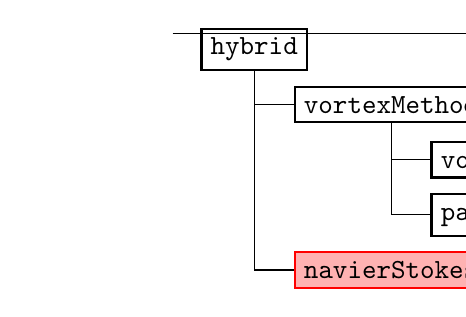
\begin{tikzpicture}[%
  grow via three points={one child at (0.5,-0.7) and
  two children at (0.5,-0.7) and (0.5,-1.4)},
  edge from parent path={(\tikzparentnode.south) |- (\tikzchildnode.west)}]
  \node {\texttt{hybrid}}
    child { node {\texttt{vortexMethod}}
    	child {node {\texttt{vortexBlobs}}}
    	child {node {\texttt{panels}}}  	
    }
    child [missing] {}				
    child [missing] {}				
    child { node [selected] {\texttt{navierStokes}}};
    %child { node [selected] {tex}
    %  child { node {generic}}
    %  child { node [optional] {latex}}
    %  child { node {plain}}
    %}
    %child [missing] {}
    %child { node {texdoc}};
\end{tikzpicture}
\end{figure}


\subsection*{Class structure:}
\begin{figure}[h]
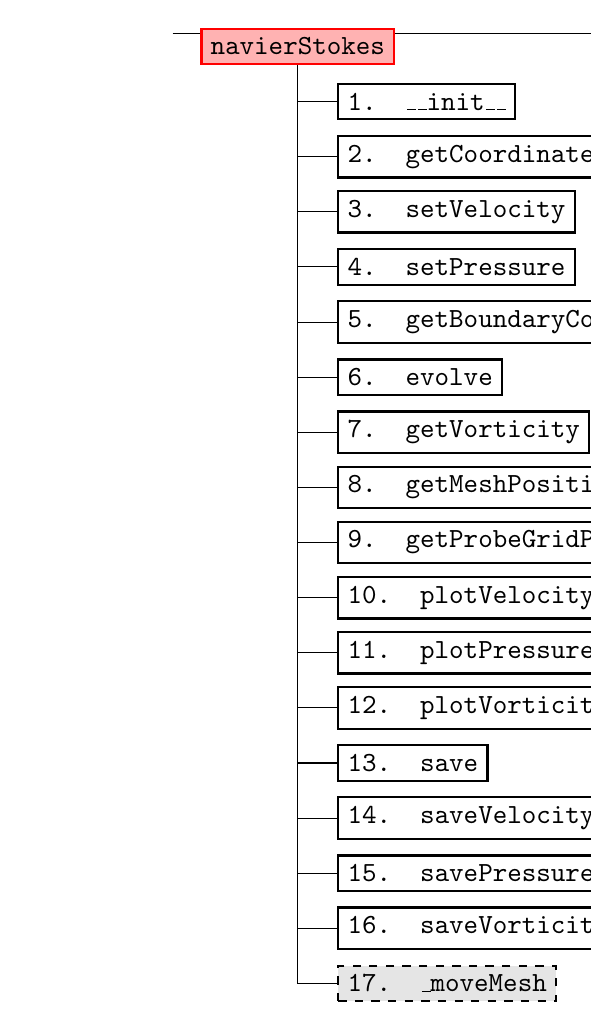
\begin{tikzpicture}[%
  grow via three points={one child at (0.5,-0.7) and
  two children at (0.5,-0.7) and (0.5,-1.4)},
  edge from parent path={(\tikzparentnode.south) |- (\tikzchildnode.west)}]
  \node [selected] {\texttt{navierStokes}}
    child { node {\texttt{1. \_\_init\_\_}}}
    child {node  {\texttt{2. getCoordinates}}}
    child { node {\texttt{3. setVelocity}}}
    child { node {\texttt{4. setPressure}}}
    child { node {\texttt{5. getBoundaryCoordinates}}}                        
    child { node {\texttt{6. evolve}}}
    child { node {\texttt{7. getVorticity}}}                        
    child { node {\texttt{8. getMeshPosition}}}                        
    child { node {\texttt{9. getProbeGridParameters}}}                        
    child { node {\texttt{10. plotVelocity}}}                        
    child { node {\texttt{11. plotPressure}}}                        
    child { node {\texttt{12. plotVorticity}}}                        
    child { node {\texttt{13. save}}}                        
    child { node {\texttt{14. saveVelocity}}}                                            
    child { node {\texttt{15. savePressure}}}                                            
    child { node {\texttt{16. saveVorticity}}}
    child { node [optional]{\texttt{17. \_moveMesh}}};
	%  child { node [selected] {tex}
    %  child { node {generic}}
    %  child { node [optional] {latex}}
    %  child { node {plain}}
    %}
    %child { node {texdoc}};
\end{tikzpicture}
\end{figure}

%\subsection*{Class structure:}
%\begin{table}[h]
%\begin{tabular}{rl}
%	\texttt{navierStokes}: &  \\ \hline
%	-- & \texttt{\_\_init\_\_} \\
%	& \\
%	-- & \texttt{initialConditions} \\ 
%	-- & \texttt{evolve} \\ 
%	-- & \texttt{boundaryCoordinates} \\ 
%	-- & \texttt{updateMesh} \\ 
%	-- & \texttt{moveMesh} \\ 
%	-- & \texttt{computeVorticity} \\ 
%	-- & \texttt{meshPosition}\\
%	-- & \texttt{probeGridParameters} \\ 	
%	-- & \texttt{plotVelocity} \\ 		
%	-- & \texttt{plotPressure} \\ 		
%	-- & \texttt{plotVorticity} \\ 			
%	-- & \texttt{saveClass} \\ 					
%	-- & \texttt{saveVelocity} \\ 		
%	-- & \texttt{savePressure} \\ 		
%	-- & \texttt{saveVorticity} \\ 	
%	-- & \texttt{saveVelocityPlot} \\ 		
%	-- & \texttt{savePressurePlot} \\ 		
%	-- & \texttt{saveVorticityPlot} \\ 	
%\end{tabular}
%%\caption{\texttt{navierStokes} class structure}
%\end{table}

\newpage

\subsection{\texttt{\_\_init\_\_}}
	\paragraph{Description:} Initialize the \texttt{navierStokes} class either using a \texttt{fileName} containing all the necessary parameter for initialization or by explicitly inputing the parameters.\\

	\begin{tabular}{l|lp{7cm}}
		\multicolumn{2}{l}{\textbf{Input Parameters}} & \\ \hline
		\textit{File Name} & \multicolumn{2}{l}{Containing all the parameters to re-initalize the class.} \\ \hline
		\multicolumn{3}{c}{-- or --} \\ \hline
		\multirow{5}{*}{\textit{Parameters}} & Mesh data &: \texttt{mesh, boundaryDomains}\\ \cline{2-3}
		& Geometry position &: \texttt{cmGlobal, thetaLocal} \\ \cline{2-3}
		& Fluid parameters &: \texttt{uMax, nu}\\ \cline{2-3}
		& Solver options &: \texttt{cfl}\\ \cline{2-3}
		& Probe grid parameters &: \texttt{x0, y0, Lx, Ly, hx, hy}\\ \cline{2-3}

	\end{tabular}\\
	\subsubsection*{Descrition of the parameters:}
	
	\begin{tabular}{lp{10cm}}
				\textit{Mesh data} & \\ \hline
				\texttt{mesh} &: the mesh data file.\\ 
				\texttt{boundaryDomains} &: the boundary mesh domain data file.\\ 			
	\end{tabular}\\ 
    \\ \\
	\begin{tabular}{lp{10cm}}
				\textit{Geometry position} & \\ \hline
				\texttt{cmGlobal} &: the $x,y$ position of the geometry in global coordinates.\\ 
				\texttt{thetaGlobal} &: the rotation angle (in $rad$) of the geometry in global coordinate system.\\ 			
	\end{tabular}\\
    \\ \\
	\begin{tabular}{lp{10cm}}
				\textit{Fluid parameters} & \\ \hline
				\texttt{uMax} &: the maximum fluid velocity $U_{max}$. Used to determine the maximum time step size $\Delta t_{max}$.\\ 
				\texttt{nu} &: the fluid kinematic viscosity $\nu$, for incompressible navier-stokes problem.\\ 			
	\end{tabular}\\	
    \\ \\
	\begin{tabular}{lp{10cm}}
				\textit{Solver options} & \\ \hline
				\texttt{cfl} &: the $CFL$ stability parameter. If explicit time marching scheme, $CFL<1$.\\ 		
	\end{tabular}\\	
    \\ \\
	\begin{tabular}{lp{10cm}}
				\textit{Probe grid parameters} & \\ \hline
				\texttt{x0,y0} &: the $x,y$ coordinate of the origin of the probe grid.\\ 
				\texttt{Lx,Ly} &: the $x,y$ size (width and height) of the probing grid.\\ 			
				\texttt{hx,hy} &: the $x,y$ spacing of the probe grid cell.\\ 							
	\end{tabular}\\	

\subsection{\texttt{getCoordinates}}
	\paragraph{Description:} Function to get all the coordinates of the velocity function spaces $\mathbf{V}$. With the returned coordinates, one could calculate the velocity field in the navier-stokes domain. \textit{Note}: The coordinates and just a list of DOF coordinate of the vector function space and is given in the same order as the data that is to be stored.\\
	
	    \begin{tabular}{lp{10cm}}
			\textit{Parameters} & \\ \hline
			\texttt{xCoordinates,yCoordinates} &: the $x,y$ coordinates of the velocity vector function space $\mathbf{V}$. \\		
		\end{tabular} \vspace{5 mm}
	\\		
	\begin{tabular}{lp{10cm}}
		\textbf{Input parameters} &: \texttt{-}\\ 
		\textbf{Assigns} &: \texttt{-}\\ 			
		\textbf{Returns} &: \texttt{xCoordinates,yCoordinates}\\ 					
	\end{tabular}

\subsection{\texttt{setVelocity}}
	\paragraph{Description:} Function to apply the current velocity field.\\
	
	    \begin{tabular}{lp{10cm}}
			\textit{Parameters} & \\ \hline
			\texttt{vFieldNew} &: the \textit{new} velocity at the navier-stokes DOF coordinates of the vector function space $\mathbf{V}$.\\		
		\end{tabular} \vspace{5 mm}
	\\		
	\begin{tabular}{lp{10cm}}
		\textbf{Input parameters} &: \texttt{vFieldNew}\\ 
		\textbf{Assigns} &: \texttt{vField}\\ 			
		\textbf{Returns} &: \texttt{-}\\ 					
	\end{tabular}
	
\subsection{\texttt{setPressure}}
	\paragraph{Description:} Function to apply the current pressure field.\\
	
	    \begin{tabular}{lp{10cm}}
			\textit{Parameters} & \\ \hline
			\texttt{pFieldNew} &: the \textit{new} pressure field at the navier-stokes DOF coordinates of the scalar function space $\mathbf{V}$.\\ 
		\end{tabular} \vspace{5 mm}
	\\		
	\begin{tabular}{lp{10cm}}
		\textbf{Input parameters} &: \texttt{pFieldNew}\\ 
		\textbf{Assigns} &: \texttt{pField}\\ 			
		\textbf{Returns} &: \texttt{-}\\ 					
	\end{tabular}

\subsection{\texttt{getBoundaryCoordinates}}
	\paragraph{Description:} Function to return the boundary DOF coordinates \texttt{xBoundary,yBoundary} of the vector function space $\mathbf{V}$.\\
	
		\begin{tabular}{lp{10cm}}
			\textit{Parameters} & \\ \hline
			\texttt{xBoundary,yBoundary} &: $x,y$ boundary coordinates of the vector function space  $\mathbf{V}$. \\ 
		\end{tabular} \vspace{5 mm}
	\\
	\begin{tabular}{lp{10cm}}
		\textbf{Input parameters} &: \texttt{-}\\ 
		\textbf{Assigns} &: \texttt{-}\\ 			
		\textbf{Returns} &: \texttt{xBoundary,yBoundary}\\ 					
	\end{tabular}	

\subsection{\texttt{evolve}}
	\paragraph{Description}: Function to evolve the Navier-stokes by one step with the $x,y$ velocity boundary condition \texttt{vxBoundary,vyBoundary} at the Navier-stokes finite element mesh boundary \texttt{xBoundary,yBoundary}. The function will calculate the new velocity and the pressure fields. The \textit{new} mesh position is used to update the mesh position, whereas the \textit{current} mesh velocity is used to calculate the modified convective term to take in account of the rigid mesh motion.\\
	
		\begin{tabular}{lp{10cm}}
			\textit{Parameters} & \\ \hline
			\texttt{vxBoundary,vyBoundary} &: $x,y$ velocity at the navier-stokes dof boundary coordinates as described by \texttt{xBoundary,yBoundary}.\\ 
			\texttt{xBoundary,yBoundary} &: $x,y$ boundary coordinates of the vector function space.\\ 
			\texttt{cmGlobalNew,thetaGlobalNew} &: the \textit{new} mesh position and the global mesh rotational angle\\
			\texttt{cmDotGlobal, thetaDotGlobal} &: the \textit{current} mesh velocities (displacement velocity and rotational velocity) in the global reference frame.\\
		\end{tabular} \vspace{5 mm}
	\\	
	\begin{tabular}{lp{10cm}}
		\textbf{Input parameters} &: \texttt{vxBoundary,vyBoundary, cmGlobalNew,thetaGlobalNew, cmDotGlobal, thetaDotGlobal}\\ 
		\textbf{Assigns} &: \texttt{vField, pField}\\ 			
		\textbf{Returns} &: \texttt{-}\\ 					
	\end{tabular}	


	

%
%\subsection{\texttt{moveMesh}}
%	\paragraph{Description:} Function to move the mesh using body displacement and rotational velocities. This function can be then used to calculate the mesh velocity of the current instant.\\
%	
%		\begin{tabular}{lp{10cm}}
%			\textit{Parameters} & \\ \hline
%			\texttt{cmDotGlobal} &: the $x,y$ global mesh coordinate displacement velocity.\\ 
%			\texttt{thetaDotGlobal} &: the polar rotational velocity of the navier-stokes domain w.r.t global coordintes.\\ 			
%			\texttt{vMesh} &: the mesh velocity w.r.t to global $x,y$-axis\\	
%		\end{tabular} \vspace{5 mm}
%	\\
%	\begin{tabular}{lp{10cm}}
%		\textbf{Input parameters} &: \texttt{cmDotGlobal,thetaDotGlobal}\\ 
%		\textbf{Assigns} &: \texttt{xBoundary,yBoundary,vMesh}\\ 			
%		\textbf{Returns} &: \texttt{-}\\ 					
%	\end{tabular}
	
	
\subsection{\texttt{getVorticity}}
	\paragraph{Description:} Function to evaluate the vorticity at probe coordinates defined by the probe mesh.\\
	
		\begin{tabular}{lp{10cm}}
			\textit{Parameters} & \\ \hline
			\texttt{vortProbeGrid} &: the vorticity $\omega$ at the probe grid coordinates \texttt{xProbeGrid, yProbeGrid}.\\ 
		\end{tabular} \vspace{5 mm}
	\\
	\begin{tabular}{lp{10cm}}
		\textbf{Input parameters} &: \texttt{-}\\ 
		\textbf{Assigns} &: \texttt{-}\\ 			
		\textbf{Returns} &: \texttt{wProbeGrid}\\ 					
	\end{tabular}


\subsection{\texttt{getMeshPosition}}

	\paragraph{Description:} Function to return the current mesh position and rotational angle.\\
	
		\begin{tabular}{lp{10cm}}
			\textit{Parameters} & \\ \hline
			\texttt{cmGlobal} &: the $x,y$ position of the mesh in global coordinates.\\ 
			\texttt{thetaGlobal} &: the rotational angle of the mesh w.r.t the global $x$ axis.\\
		\end{tabular} \vspace{5 mm}
	\\
	\begin{tabular}{lp{10cm}}
		\textbf{Input parameters} &: \texttt{-}\\ 
		\textbf{Assigns} &: \texttt{-}\\ 			
		\textbf{Returns} &: \texttt{cmGlobal,thetaGlobal}\\ 					
	\end{tabular}

\subsection{\texttt{getProbeGridParameters}}

	\paragraph{Description:} Function to return the probe grid parameters.\\
	
		\begin{tabular}{lp{10cm}}
			\textit{Parameters} & \\ \hline
			\texttt{x0,y0} &: the global $x,y$ coordinates of the probe mesh origin.\\ 
			\texttt{Lx,Ly} &: the local width and height of the probe mesh.\\
			\texttt{hx,hy} &: the probe spacing of the structure probe mesh.\\			
		\end{tabular} \vspace{5 mm}
	\\
	\begin{tabular}{lp{10cm}}
		\textbf{Input parameters} &: \texttt{-}\\ 
		\textbf{Assigns} &: \texttt{-}\\ 			
		\textbf{Returns} &: \texttt{x0,y0,Lx,Ly,hx,hy}\\ 					
	\end{tabular}

\subsection{plots \ldots}
	\paragraph{Description:} Function to plot and/or save (\textit{optional}) all the results.\\
	
		\begin{tabular}{lp{10cm}}
			\textit{Plot variables} & \\ \hline
			\texttt{plotVelocity} &: the velocity $\mathbf{V}$ of the navier-stokes domain, \texttt{u1}.\\ 
			\texttt{plotPressure} &: the pressure $\mathbf{p}$ of the navier-stokes domain, \texttt{p1}\\ 
			\texttt{plotVorticity} &: the vorticity $\mathbf{\omega}$ of the navier-stokes domain, \texttt{w1}.\\ 
		\end{tabular} \vspace{5 mm}
	\\
	\begin{tabular}{lp{10cm}}
		\textbf{Input parameters} &: \texttt{-}\\ 
		\textbf{Assigns} &: \texttt{-}\\ 			
		\textbf{Returns} &: \texttt{figureHandle} or \texttt{saveFile}\\ 					
	\end{tabular}

\subsection{save datas \ldots}
	\paragraph{Description:} Function to save the navier-stokes data as binaries.\\
	
		\begin{tabular}{lp{10cm}}
			\textit{Save variables} & \\ \hline
			\texttt{save} & : all the data of the \texttt{navierStokes} class, to be used to restart later.\\
			\texttt{saveVelocity} &: the velocity $\mathbf{V}$ of the navier-stokes domain, \texttt{u1}.\\ 
			\texttt{savePressure} &: the pressure $\mathbf{p}$ of the navier-stokes domain, \texttt{p1}\\ 
			\texttt{saveVorticity} &: the vorticity $\mathbf{\omega}$ of the navier-stokes domain, \texttt{w1}.\\ 
		\end{tabular} \vspace{5 mm}
	\\
	\begin{tabular}{lp{10cm}}
		\textbf{Input parameters} &: \texttt{-}\\ 
		\textbf{Assigns} &: \texttt{-}\\ 			
		\textbf{Returns} &: \texttt{.npz}\\ 					
	\end{tabular}

\subsection{\texttt{\_moveMesh}}
	\paragraph{Description:} \textit{Internal} function to update the mesh coordinates using the new global position and rotational angle of the body. The function will be called through \texttt{evolve}.\\
	
		\begin{tabular}{lp{10cm}}
			\textit{Parameters} & \\ \hline
			\texttt{cmGlobal} &: the $x,y$ global coordinates of the body.\\ 
			\texttt{thetaGlobal} &: the polar rotational angle of the navier-stokes domain w.r.t global $x$-coordinate axis.\\ 			
		\end{tabular} \vspace{5 mm}
	\\
	\begin{tabular}{lp{10cm}}
		\textbf{Input parameters} &: \texttt{cmGlobal,thetaGlobal}\\ 
		\textbf{Assigns} &: \texttt{xBoundary,yBoundary}\\ 			
		\textbf{Returns} &: \texttt{-}\\ 					
	\end{tabular}


%\subsection{save plots \ldots}
%	\paragraph{Description:} Function to save the navier-stokes plots are scientific visualization format \texttt{.pvd}.\\
%	
%		\begin{tabular}{lp{10cm}}
%			\textit{Save variables} & \\ \hline
%			\texttt{saveVelocityPlot} &: the velocity $\mathbf{V}$ plot of the navier-stokes domain, \texttt{u1}.\\ 
%			\texttt{savePressurePlot} &: the pressure $\mathbf{p}$ plot of the navier-stokes domain, \texttt{p1}\\ 
%			\texttt{saveVorticityPlot} &: the vorticity $\mathbf{\omega}$ plot of the navier-stokes domain, \texttt{w1}.\\ 
%		\end{tabular} \vspace{5 mm}
%	\\
%	\begin{tabular}{lp{10cm}}
%		\textbf{Input parameters} &: \texttt{-}\\ 
%		\textbf{Assigns} &: \texttt{-}\\ 			
%		\textbf{Returns} &: \texttt{.pvd}\\ 					
%	\end{tabular}
%\chapter{Hybrid Eulerian-Lagrangian Vortex Particle Method}
\label{ch:helvpm}

% Summarize the sections. : domain decomposition, coordinate systems assosciated to each
% subdomains, and the coupled evolution of the hybrid method.
% Reference to the literatures: Cottet and others, stock and daenick
% We use approach of stock based on the phd research of daeninck

	\section{Introduction to Hybrid Eulerian-Lagrangian Vortex Particle Method}
	
	The \printAcron{Hybrid Eulerian-Lagrangian Vortex Particle Method}{HELVPM} is a domain decomposition method, where the Eulerian method and the Lagrangian method solves different regions of the fluid. The domain decomposition method simply splits the domain of interest and uses appropriate method in each domain. The Eulerian formulation will be used at the near-wall region, where we need proper description of the vorticity generation at the boundary, and the Lagrangian formulation is used away from the body, where we only need to evolve the vorticity field. Figure \ref{fig:domainDecomposition} shows the decomposition of the domain to the gridded and the non-gridded region.
	
		\begin{figure}[!h]
			\centering
			\includegraphics[width=0.6\linewidth]{figures/hybrid/domainDecomposition_typical_type2-crop.pdf}
			\caption{Standard domain decomposition using Schwartz iteration for coupling the two methods. Eulerian subdomain $\Omega_E$ (near the body), and Lagrangian subdomain $\Omega_L$ (away from the body). Figure is based on Guermond (2000) \cite{Guermond2000a}.}
			\label{fig:domainDecomposition}
		\end{figure}	
	
	Several studies have already been done: Cottet and Koumoutsakos (2000a)\cite{Cottet2000a}, Guermond and Lu (2000) \cite{Guermond2000a} simulated the advection dominated flows; Ould-Salhi et al. (2001) \cite{Ould-Salihi2001a} blended the finite difference and vortex method together; Winckelmans et al. (2005a) \cite{Winckelmans2005} investigated the trailing vorticies; Daeninck (2006) \cite{Daeninck2006} used a simplified coupling strategy, coupling Vortex Particle Method and Finite Diference Method; Stock (2010) \cite{Stock2010a} expanded Daeninck's strategy, coupling Vortex Particle Method and Finite Volume Method and modeled a 3D rotor.

	\section{Convectional Coupling Strategy}
	\label{sec:helvpm-ccs}
	
	When investigating the literature works, we see that not all domain decomposition methods are the same. The main difference between the methods is their coupling strategies. Most works employ the\textit{ Schwartz alternating method} to couple the vortex particle method and the grid solver. The Schwartz alternating method (or sometimes referred to as Schwartz iterative method), couples the vortex particle method and the grid solver by iteratively determining the boundary condition such that the stream functions in both domains, $\psi_L$ and $\psi_E$ in $\Omega_L$ and $\Omega_E$ respectively, match at the overlap region $\Omega_E-\Omega_L$, shown in Figure \ref{fig:domainDecomposition}. The summary of a single iteration of the Schwartz alternating method is as follows:
	
		\begin{itemize}
		\item Determine the Eulerian boundary condition, the stream function $\psi_{\Sigma_1}$ at the Eulerian boundary $\Sigma_1$, extracted from the Lagrangian stream function $\psi_L$ in the Lagrangian subdomain $\Omega_L$.
		\item Solve for the stream function $\psi_E$ in the Eulerian subdomain $\Omega_E$ with the new boundary condition $\Sigma_1$.
		\item Determine the Lagrangian condition, the stream function $\psi_{\Sigma_0}$ at the Lagrangian boundary $\Sigma_0$, extracted from the Eulerian stream function $\psi_E$ in the Eulerian subdomain $\Omega_E$.
		\item Solve the stream function $\psi_L$ in the Lagrangian subdomain with the boundary conditions $\psi_{\Sigma_0}$ at the Lagrangian boundary $\Sigma_0$.
		\end{itemize}
	
	This procedure is iterated until the stream functions of both domains converge \cite{Ould-Salihi2001a}. Once the stream function is determined in both the domains, the velocity field can be obtained. Using the velocity field, we can then evolve the vorticity field in the Lagrangian subdomain.

	\section{Simplified Coupling Strategy}
	\label{sec:helvpm-scs}
	
	As we realized now, the downside to this procedure is that we have to solve the stream function in both $\Omega_E$ and $\Omega_L$ iteratively, until we converge to a solution. This makes the computation very expensive, especially when we are dealing with large numbers of vortex particles. Therefore, for this project, we are using the coupling technique that is based on the research work of Daeninck (2006) \cite{Daeninck2006} and Stock (2010) \cite{Stock2010a}. However, through the course of present work, we will see that we have to perform a modification to the scheme, to ensure that the total circulation of the Lagrangian domain is conserved at all times.	
	
%	\subsection{Coupling Eulerian and Lagrangian Methods}
	
	The simplified coupling strategy was first demonstrated in the doctoral thesis of Daeninck \cite{Daeninck2006}. Daeninck showed that it is possible to coupled the Lagrangian and the Eulerian method without the use of Schwartz iterative method. Daeninck proposed this approach from the following statements:
	
	\begin{itemize}
	\item The Lagrangian vortex method solves the full fluid domain $\Omega_L$ (see Figure \ref{fig:domainDecomposition_daenick}), but under-resolves the near-wall region $\Omega_E$ as it is less efficient at resolving the boundary layer of the flow.
	
	\item Eulerian method is used to resolve the near-wall region $\Omega_E$, efficiently capturing the boundary layer features and flow separation.
	
	\item The Lagrangian subdomain in the near-wall region $\Omega_L\cap\Omega_E$ is corrected using the more accurate Eulerian solutions to compensate the aforementioned under-resolution.
	
	\item The boundary conditions for the Eulerian method is directly obtained from the evolved solution of the Lagrangian method.
	\end{itemize}
	
	The grid solver therefore essentially acts as the correction for the under-resolved regions of the Lagrangian method. The Lagrangian vortex method in the full fluid domain focuses only on capturing and efficiently evolving the wake.
	
		\begin{figure}[!h]
			\centering
			\includegraphics[width=0.6\linewidth]{figures/hybrid/domainDecomposition_daenick_type2-crop.pdf}
			\caption{Modified domain decomposition \underline{without} Schwartz alternating method. Lagrangian subdomain extends up to the surface of the body. Figure is based on Daeninck (2006) \cite{Daeninck2006}.}
			\label{fig:domainDecomposition_daenick}
		\end{figure}	
	
	Furthermore, Daeninck's simplified coupling strategy handles the Lagrangian boundary condition differently from the convectional domain decomposition method. In convectional method, the shedding of the vorticity from the wall is also defined in the Lagrangian method as well. However, in Daeninck's strategy, as the Lagrangian method is under-resolved at the boundary, it cannot be used to resolve the vorticity flux at the body. Instead, the Eulerian method is used to solve vorticity generation from the wall boundary, and acts as the vorticity generator for the Lagrangian method. 
	
	For this coupling strategy to be valid, there are some assumptions that we must satisfy:

	\begin{itemize}
	\item At $t_n$ before the evolution of both method to $t_{n+1}$, the Lagrangian solution matches Eulerian solution at the boundary of the near-wall region $\Sigma_d$ (see Figure \ref{fig:domainDecomposition_daenick}).
	\item Even though the Lagrangian subdomain is under-resolved in the near-wall region, it should still be able to provide accurate boundary conditions for the Eulerian method at the external boundary $\Sigma_d$.
	\item After the evolution to $t_{n+1}$, the deviation of the Lagrangian solution (due to lack of vorticity flux at Lagrangian boundary), should be minimal.
	\end{itemize}	
	
	Daeninck's the simplified coupling strategy focused on the vorticity-velocity formulation for the Eulerian domain. However, he briefly showed that it is also possible to couple the Eulerian method with the velocity-pressure formulation. The advantage of using the velocity-pressure formulation is that it will be easier to extend to a 3D problem, unlike the vorticity-velocity formulation for the Eulerian method.
	
	\subsection{Coupling Algorithm}	
	
	The coupling of the solvers was described in one global time stepping algorithm. As the Eulerian methods suffers from a larger stability constraint on the time step, and the Lagrangian time marching is computationally more expensive, a  different time discretization for both methods was employed. The Lagrangian method and the Eulerian method had the time steps $\Delta t_L$ and $\Delta t_E=\Delta t_L/k_E$, respectively, where $k_E$ is the number of Eulerian sub-steps.
	
	Assuming that we known the solutions of both solver at $t_n$, the algorithm for the coupled time marching from $t_n$ to $t_n+\Delta t_L$ for Eulerian method (with velocity-pressure formulation) and the Lagrangian method is summarized as follows:
	
	\begin{enumerate}
	\item At $t_n$, \textbf{correct the Lagrangian solution} in the near-wall region $\Omega_L\cap\Omega_E$ from the Eulerian field, Figure \ref{fig:domainDecomposition_daenick}. The vorticity in $\Omega_E$ is determined by taking the curl of the velocity field of the Eulerian method. The vortex particles strengths are determined by interpolating the vorticity from the Eulerian grid.
	
	\item \textbf{Advance the Lagrangian method} from $t_n$ to $t_{n}+\Delta t_L$, with the corrected Lagrangian solution. Before the evolution, there exists a slip velocity at the solid wall $\Sigma_w$. Therefore, the vortex method needs to enforce the \textit{no-slip} boundary condition at the wall by computing the vortex sheet $\gamma$ that cancels this slip velocity. At the end of the evolution, classic vortex methods diffuse the computed vortex sheet to the particles but in Daeninck's work, it is handled by the Eulerian method.
	
	\item\textbf{ Determine the Eulerian boundary conditions} for the velocity field $\mathbf{u}$ at $t_{n}+\Delta t_L$ from the Lagrangian solution at $t_{n} + \Delta t_L$. The Eulerian method requires the Dirichlet velocity boundary condition at $\Sigma_d$ (the Eulerian Dirichlet velocity boundary). The velocity boundary condition at the wall boundary $\Sigma_w$ for a velocity-pressure formulation is simply the zero slip velocity. 
	
	\item \textbf{Advance the Eulerian method} from $t_n$ to $t_n + \Delta t_L$ using $k_E$ Eulerian substeps. The boundary conditions on $\mathbf{u}$ at each substep is obtained by linear interpolation of the boundary condition at $t_n$ and $t_{n} + \Delta t_L$.
	\end{enumerate}	
	
	To enhance the coupling of the Eulerian and the Lagrangian method, Daeninck further modified the Eulerian solution in the most external region of the Eulerian subdomain $\Omega_E$ from interpolation the Lagrangian solution, and observed that it provided better results. Figure \ref{fig:daeninckInterpolation} the modified adjustments regions used by Daeninck in his work.
	
	\begin{figure}[!t]
		\centering
		\includegraphics[width=0.6\linewidth]{figures/hybrid/daeninckInterpolationRegions.png}
		\caption{The domain decomposition and interpolation regions used by Daeninck \cite{Daeninck2006}. The Eulerian domain is also modified to enchace the coupling of the methods.}
		\label{fig:daeninckInterpolation}
	\end{figure}		
	
	\subsection{Lagrangian Correction Step}
	
	The coupling strategy demonstrated by Daeninck \cite{Daeninck2006}, was studied and was further extended by Stock \cite{Stock2010a}. Stock's work focused on the overlap region $\Omega_E\cap\Omega_L$ (Figure \ref{fig:domainDecomposition_daenick}) and correction of the Lagrangian solution. Following observations was determined by the work:
	
	\begin{itemize}
	\item Eulerian solution is only assumed to be correct from the body surface $\Sigma_w$ to somewhat inside of the outer Eulerian domain $\Sigma_d$. Therefore, the transfer of the Eulerian solution to the Lagrangian method should take in account of the potential inaccuracy of the Eulerian solution at the outer boundary.
	
	\item The very strong gradient in vorticity (vortex sheet) cannot be efficiently and accurately transfered to the Lagrangian method. This is especially problematic at high Reynolds number flows, and interpolating this vorticity from Eulerian method to Lagrangian method results in numerical problems. Therefore, to avoid the noise in the interpolation, the correction step has to ignore the region very near to the wall.
	\end{itemize}
	
	The resulting Lagrangian correction domain, or the interpolation domain $\Omega_I$, using Stock's coupling approach is shown in Figure \ref{fig:interpolationDomainDefinition}. The interpolation domain $\Omega_I$ is defined with an offset from the Eulerian domain boundaries $\Omega_E: \partial\Omega_E=\Sigma_w \cup \Sigma_d$, Figure \ref{fig:interpolationDomainExpanded}, such that regions of the Eulerian domain that introduces issues with coupling are ignored. The outer boundary of the interpolation domain $\Sigma_i$ is defined with an offset $d_{bdry}$ from the Eulerian Dirichlet velocity boundary $\Sigma_d$ such that potential inaccuracy of the Eulerian solution is ignored, shown in Figure \ref{fig:interpolationDomainCloseup}. Similarly, the inner boundary of the interpolation domain $\Sigma_o$ is defined with an offset $d_{surf}$ from the Eulerian wall boundary $\Sigma_w$ such that the very strong vorticity is ignored. The offsets $d_{surf}$ and $d_{bdry}$  where defined in the order of the Lagrangian vortex particle size.
	
	\begin{figure}[!t]
        \centering
        \begin{subfigure}[b]{0.45\textwidth}
                \includegraphics[width=\textwidth]{figures/hybrid/interpolationDomain/interpolationDomainExpanded-crop.pdf}
                \caption{Definition of the Domains}
                \label{fig:interpolationDomainExpanded}
        \end{subfigure}%
        \qquad %add desired spacing between images, e. g. ~, \quad, \qquad etc.
          %(or a blank line to force the subfigure onto a new line)
        \begin{subfigure}[b]{0.45\textwidth}
                \includegraphics[width=\textwidth]{figures/hybrid/interpolationDomain/interpolationDomainCloseup-crop.pdf}
                \caption{Definition of the boundaries}
                \label{fig:interpolationDomainCloseup}
        \end{subfigure}
        \caption{Definition of the interpolation domain $\Omega_{int}$ for correcting the Lagrangian solution, with boundaries $\Omega_I: \partial\Omega_I=\Sigma_{i}\cup\Sigma_{o}$.}
        \label{fig:interpolationDomainDefinition}
	\end{figure}		

	The resulting Lagrangian correction step employed by Stock is summarized as follows:
	
	\begin{enumerate}
	\item Interpolate the vorticity of the Eulerian method from a non-uniformly structured (or an unstructured grid) onto a temporary uniformly structured Cartesian grid covering the entire Eulerian domain $\Omega_E$. This is done to performed an easier correction of the Lagrangian solution with the Eulerian solution. The interpolation ignores the very strong vorticity present in the boundary layer that could cause numerical problem.
	\item Determine all the particles within the interpolation domain $\Omega_I$ that is to be corrected.
	\item Correct or reset the strengths of the particles using the local particle area and the vorticity interpolated from the temporary structured Cartesian grid.
	\end{enumerate}
	
	Using this approach, Stock demonstrated the feasibility of simulating a 3D compressible flow problem around a sphere at $Re=100$, a finite airfoil at $Re=\num{1.5e6}$, and 4-Bladed advancing rotor at $Re=865,500$.
	
	\section{Evolution of the Hybrid Method}

	In the present work, we will therefore employ Daeninck's simplified coupling strategy with the detailed Lagrangian correction approach of the Stock. The evolution of the hybrid method is classified into four parts and is as follows:

		\begin{enumerate}
		\item \textbf{Correct Lagrangian:} Use the solution of the Eulerian subdomain $\Omega_E$, to correct the solution of the Lagrangian subdomain $\Omega_L$, using the strategy of Stock. Chapter \ref{ch:coupling} provides a detailed investigation on the implementation of Stock's Lagrangian correction strategy. However, during the implementation, we saw that conservation of total circulation in the Lagrangian method is paramount for an accurate correction.
		
		\item \textbf{Evolve Lagrangian:} With the modified solution, evolve the Lagrangian solution from time step $t_n$ to $t_{n}+\Delta t_L$. Chapter \ref{ch:lagrangian} provides the detailed investigation on the theory and the algorithm of the Lagrangian method used for the present work.
		
		\item \textbf{Determine Eulerian boundary conditions:} Use the Lagrangian solution of time $t_{n}+\Delta t_L$ to determine the boundary conditions of the Eulerian subdomain at $t_{n}+\Delta t_L$.
		
		\item \textbf{Evolve Eulerian:} With the boundary condition, evolve the Eulerian solution from $t_n$ to $t_{n}+\Delta t_L$ using $k_E$ Eulerian substeps. Chapter \ref{ch:eulerian} provides the detailed investigation on the theory and the algorithm of the Eulerian method used for the present work.
		\end{enumerate}
	
	Figure \ref{fig:flowchart_simpleCoupling} shows the flowchart of the evolution of the hybrid method. To ensure that the coupling of the hybrid method performs as explained in theory, we required a verification and validation test on the functionality of each segregate methods.
	
	
	\begin{figure}[!t]
		\centering
		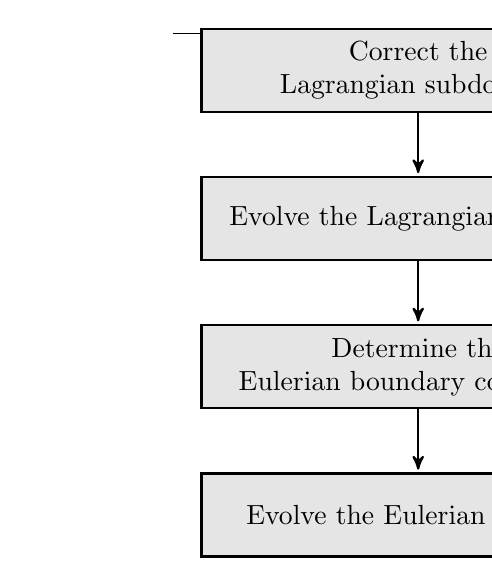
\begin{tikzpicture}
			[node distance=.8cm, start chain=going below,]
			\node[punktchain, join] (correct) {Correct the \\Lagrangian subdomain};
		    \node[punktchain, join] (evolveL) {Evolve the Lagrangian solution};
		    \node[punktchain, join] (bcE)     {Determine the \\Eulerian boundary conditions};
		    \node[punktchain, join] (evolveE) {Evolve the Eulerian solution};
		\end{tikzpicture}
		\caption{Flowchart of the simple coupling strategy. The flowchart shows the procedure to evolve both methods from $t_n$ to $t_{n+1}$.}
		\label{fig:flowchart_simpleCoupling}
	\end{figure}




% Summarize daenincks approach:
	% Methodology, algorithm
	% Domain decomposition
% Summarize stock's approach:
	% Methodology, algorithms
	% Resulted domain decomposition.


%%%%%%%%%%%%%%%%%%%%%%%%%%%%%%%%%%%%%%%%%%%%%%%%%%%%%%%%%%%%%%%%%%%%%%%%%%%%%%%%%%%%%%%%%%%%%%%%%%%%%%%%%%%%%%%%%%%%%%%%%%%%%%%%%%



%
    	
%    \appendix  
%    \addcontentsline{toc}{chapter}{Appendix}
%   	
\chapter{\texttt{pHyFlow} Code Structure}
\label{app:code}%

% Tikz stypes
\tikzstyle{every node}=[draw=black,thick,anchor=west]
\tikzstyle{optional}=[dashed,fill=gray!20]
\tikzstyle{selected}=[draw=red,fill=red!30]


%\title{pHyFlow Code Structure}
%\author{Artur Palha, Lento Manickathan}

%\begin{document}
%\maketitle
%\begin{abstract}
The document outlines the \texttt{pHyFlow} code structure. The \texttt{pHyFlow} functions are organized into several classes. The functions related to the vortex particles are placed inside the \texttt{Blobs} class. The functions related to the panel problem are inside \texttt{Panels} class. The \texttt{LagrangianSolver} class is made to couple the functions of the vortex blobs and the vortex panel together. The functions of the Eulerian domain are placed inside the \texttt{EulerianSolver} class, where the Navier-stokes grid problem is solved. Finally, coupling of all the problems are done with the \texttt{HybridSolver} class. Note, all the classes are capable of handling multi-body / multi-domain problem within them and \texttt{LagrangianSolver} class and the \texttt{HybridSolver} class only couples methods together.\\

\underline{\texttt{pHyFlow} Structure:}
\begin{figure}[h]
\centering
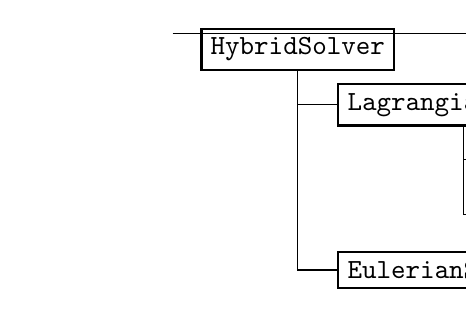
\begin{tikzpicture}[%
  grow via three points={one child at (0.5,-0.7) and
  two children at (0.5,-0.7) and (0.5,-1.4)},
  edge from parent path={(\tikzparentnode.south) |- (\tikzchildnode.west)}]
  \node {\texttt{HybridSolver}}
    child { node {\texttt{LagrangianSolver}}
    	child {node {\texttt{Blobs}}}
    	child {node {\texttt{Panels}}}  	
    }
    child [missing] {}				
    child [missing] {}				
    child { node {\texttt{EulerianSolver}}};
    %child { node [selected] {tex}
    %  child { node {generic}}
    %  child { node [optional] {latex}}
    %  child { node {plain}}
    %}
    %child [missing] {}
    %child { node {texdoc}};
\end{tikzpicture}
\end{figure}
%\end{abstract}
\newpage

\section*{\texttt{Blobs} Class}
The main structure of the \texttt{Blobs} class. This class contains all the function related to the calculation of the vortex blobs.
\begin{figure}[h]
\centering
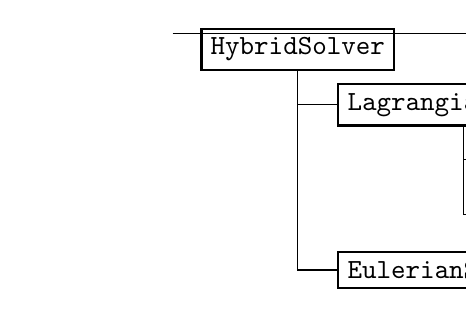
\begin{tikzpicture}[%
  grow via three points={one child at (0.5,-0.7) and
  two children at (0.5,-0.7) and (0.5,-1.4)},
  edge from parent path={(\tikzparentnode.south) |- (\tikzchildnode.west)}]
  \node {\texttt{HybridSolver}}
    child { node {\texttt{LagrangianSolver}}
    	child {node [selected] {\texttt{Blobs}}}
    	child {node {\texttt{Panels}}}  	
    }
    child [missing] {}				
    child [missing] {}				
    child { node {\texttt{EulerianSolver}}};
    %child { node [selected] {tex}
    %  child { node {generic}}
    %  child { node [optional] {latex}}
    %  child { node {plain}}
    %}
    %child [missing] {}
    %child { node {texdoc}};
\end{tikzpicture}
\end{figure}

\subsection*{Class structure:}
\begin{figure}[h]
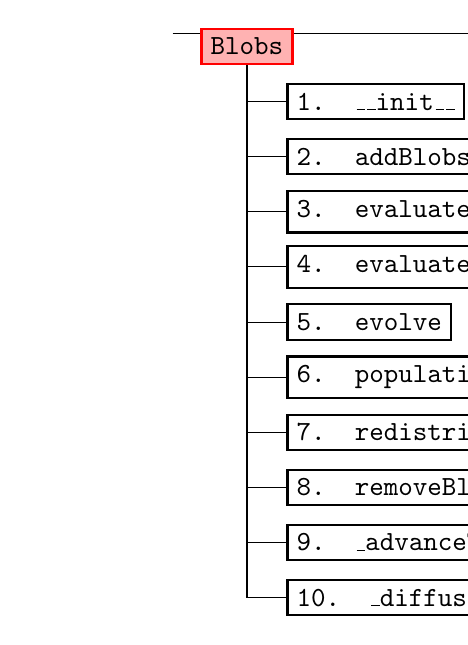
\begin{tikzpicture}[%
  grow via three points={one child at (0.5,-0.7) and
  two children at (0.5,-0.7) and (0.5,-1.4)},
  edge from parent path={(\tikzparentnode.south) |- (\tikzchildnode.west)}]
  \node [selected] {\texttt{Blobs}}
    child { node {\texttt{1. \_\_init\_\_}}}
    child { node {\texttt{2. addBlobs}}}
    child { node {\texttt{3. evaluateVelocity}}}                    
    child { node {\texttt{4. evaluateVorticity}}}   
    child { node {\texttt{5. evolve}}}    
    child { node {\texttt{6. populationControl}}}   
    child { node {\texttt{7. redistribute}}}    
	child { node {\texttt{8. removeBlobs}}}  
	child { node {\texttt{9. \_advanceTime}}}  	
	child { node {\texttt{10. \_diffusion}}};	
\end{tikzpicture}
\end{figure}

\subsection*{Attributes:}
\begingroup
\footnotesize
\begin{longtable}{|l|p{9cm}|}
	\hline
	\textbf{Attributes} & \textbf{Description}\\
	\toprule
    \texttt{blobControlParams} 		& The diffusion parameters. It is a dictionary containing all the parameters of the diffusion method used for the simulation. Contains: \texttt{stepRedistribution}, \texttt{stepPopulationControl}, \texttt{gThresholdLocal}, \texttt{gThresholdGlobal}.\\\hline
    \texttt{computationMethod} 		&\texttt{computationMethod} (tuple) with the type of Biot-Savart solver (\texttt{direct}, \texttt{fmm}) and the type of hardware to use (\texttt{cpu}, \texttt{gpu}).\\\hline
    \texttt{deltaTc} & The size of the convective time step $\Delta t_c$\\\hline
    \texttt{deltaTd} & The size of the convective time step $\Delta t_d$\\\hline
    \texttt{diffusionParams} & A dictionary containing all the parameters related to the computation of the diffusion step. Specifies the diffusion scheme and other specific parameters. Contains: \texttt{method}, \texttt{c2}.\\\hline
    \texttt{g} & The strength of the vortex blobs $\alpha$.\\          \hline
    \texttt{gThresholdGlobal} & Maximum value of variation of total vorticity due to the removal of blobs during population control.\\\hline
    \texttt{gThresholdLocal} & Minimum value of circulation to consider for each vortex blob when selecting blobs to remove during population control.\\    \hline      
    \texttt{h} & The size of the cell associated to the vortex blobs. Corresponds to the minimum spacing between the core of two neighboring cells. It is related to the core size of the blob, $\sigma$, and to the spacing $h$ by the expression $Ov = h/\sigma$.\\\hline          
    \texttt{integrationMethod} & \texttt{integrationMethod} (\texttt{fe}, \texttt{rk4}) the type of time integrator used: \texttt{fe} forward Euler, \texttt{rk4} Runge-Kutta $4^{th}$ order.\\ \hline
    \texttt{nu} & The fluid kinematic viscosity, used to calculate the diffusion coefficient: \texttt{c2} and diffusion time step \texttt{deltaTd}, $\Delta t_{d}$.\\          \hline
	\texttt{numBlobs} & The number of blobs.\\          \hline
	\texttt{overlap} & The overlap ratio between neighboring blobs.\\          \hline
	\texttt{plotVelocity} & A flag that defines if velocity is to be plotted or not.\\          \hline
	\texttt{sigma} & The core size of the vortex blobs.\\          \hline
	\texttt{stepDiffusion} & The frequency of diffusion steps.\\          \hline
	\texttt{stepPopulationControl} & The frequency of population control.\\          \hline
	\texttt{stepRedistribution} & The frequency of redistribution of blobs.\\          \hline
	\texttt{timeIntegrationParams} & A dictionary containing all time integration parameters of the simulation. Contains the definition of the time integration scheme possibly additional parameters specific to the scheme.\\ \hline
	\texttt{t} & The current time of the simulation.\\          \hline
	\texttt{tStep} & The current time step of the simulation.\\          \hline
	\texttt{velocityComputationParams} & A dictionary containing all the parameters related to the computation of induced velocities. Specifies computation scheme (direct or fmm) and hardware to use (cpu or gpu).\\          \hline
	\texttt{vInf} & The free stream velocity.\\          \hline
	\texttt{x} & The $x$ coordinates of the vortex blobs.\\          \hline
	\texttt{y} & The $y$ coordinates of the vortex blobs.\\          \hline	                                
    
                       
    \caption{Attributes of \texttt{Blobs} class and their description.}
    \label{tab:attributeBlobs}
\end{longtable}
\endgroup

\subsection*{\texttt{\_\_init\_\_}}
	\paragraph{Description:} Initialize the \texttt{Blobs} class with either the given input parameters or by a reading a \texttt{file} containing all the necessary parameters.\\
	
	\begin{tabular}{l|lp{7cm}}
		\multicolumn{2}{l}{\textbf{Input Parameters}} & \\ \hline
		\textit{File Name} & \multicolumn{2}{l}{Containing all the parameters to re-initalize the class.} \\ \cline{2-3}
		\multicolumn{3}{c}{--- or ---} \\ \cline{2-3}
		\multirow{4}{*}{\textit{Parameters}} & Vorticity Field &: \{\texttt{xBlob, yBlob, gBlob}\} or \{\texttt{wFunction, xBounds, yBounds}\}\\ \cline{2-3}
		& Blob parameters &: \texttt{overlap, h} \\ \cline{2-3}
		& Time Step parameters &: \texttt{deltaTc, nu, stepRedistribution, integrationMethod, computationMethod}\\ \cline{2-3}
		& Population control parameters &: \texttt{stepPopulationControl, gThreshold}\\ \cline{2-3}
	\end{tabular}\\
	
	\subsubsection*{Descriptions of the parameters:}
	\begin{tabular}{p{3.5cm}p{9cm}p{1cm}}
				\textit{Vorticity field} & & \textit{Default}\\ \hline
				\texttt{xBlob,yBlob} &:  the $x,y$ blob coordinates. & - \\
				\texttt{gBlob} &: the circulation $\Gamma_i$ associated to each of the vortex blobs. & - \\
				& & \\
				\multicolumn{2}{c}{\textit{--- or ---}} & \\
				& & \\
				\texttt{wExactFunction} &: the function that returns the exact value of vorticity $\omega$ at any given $x,y$ coordinates. &\\
				& 	\begin{tabular}{lp{10cm}}
						\textbf{Input parameters} &: \texttt{xEval,yEval}\\ 
						\textbf{Assigns} &: \texttt{-}\\ 			
						\textbf{Returns} &: \texttt{wEval}\\ 					
					\end{tabular} & - \\
				\texttt{xBounds, yBounds} &: the $x,y$ bounds of the domain where the particles was originally distributed. & - \\		 
	\end{tabular}\\
	\\ \\
	%	\begin{tabular}{lp{10cm}}
	%		\textbf{Input parameters} &: \texttt{xEval,yEval}\\ 
	%		\textbf{Assigns} &: \texttt{-}\\ 			
	%		\textbf{Returns} &: \texttt{vortEval}\\ 					
	%	\end{tabular}\\
	\begin{tabular}{p{3.5cm}p{9cm}p{1cm}}
				\multicolumn{2}{l}{\textit{Blob parameters}} & \textit{Default} \\ \hline				
				\texttt{overlap} &: the overlap ratio $h/\sigma$. & 1.0\\
				\texttt{h} &: the size of the cell $h$ associated to the blobs. \textit{Note:} Cells are square. & -\\
	\end{tabular}\\
	\\ \\
	\begin{tabular}{p{3.5cm}p{9cm}p{1cm}}
				\multicolumn{2}{l}{\textit{Time step parameters}} & \textit{Default}\\ \hline
				\texttt{deltaTc} &:  the size of the convective time step $\Delta t_c$. & - \\
				\texttt{nu} &: the fluid kinematic viscosity $\nu$, used to calculate the diffusion coefficient $c^2$ and diffusion time step size $\Delta T_d$.& - \\
				\texttt{stepRedistribution} &: the redistribution step frequency. & 1 \\
				\texttt{integrationMethod} &: the time integration method (\texttt{FE}: Forward euler , \texttt{RK4}: $4^{th}$ order Runge-Kutta). & RK4 \\
				\texttt{computationMethod} &: the calculation method to evolve the blobs, (\texttt{Direct}: Direct Method, \texttt{FMM}: Fast-Multipole Method) using (\texttt{CPU}, \texttt{GPU}). & \{FMM, GPU\}.\\
	\end{tabular}\\ 
    \\ \\ 
	\begin{tabular}{p{3.5cm}p{9cm}p{1cm}}
				\multicolumn{2}{l}{\textit{Population control parameters}} & \textit{Default} \\ \hline
				\texttt{stepPopulationControl} &: population control step frequency & 1.\\
				\texttt{gThreshold} &: the tuple with minimum \textbf{and} maximum value of the circulation $\Gamma_{min}$. & - \\
	\end{tabular}\\ 
    \\ \\  
	\begin{tabular}{p{3.5cm}p{9cm}p{1cm}}
				\multicolumn{2}{l}{\textit{Free stream velocity}} & \textit{Default}\\ \hline
				\texttt{vInf} &: The free-stream velocity function, returning the velocity action on the vortex blobs. & -\\		
				&		\begin{tabular}{lp{2cm}}
							\textbf{Input parameters} &: \texttt{t}\\ 
							\textbf{Assigns} &: \texttt{-}\\ 			
							\textbf{Returns} &: \texttt{vx,vy}\\ 					
						\end{tabular} & - \\
				
	\end{tabular}\\

\newpage
%%%%%%%%%%%%%%%%%%%%%%%%%%%%%%%%%%%%%%%%%%%%%%%%%%%%%%%%%%%%%%%%%%%%%%%%%%%%%%%%%%%%%%%%%%%%%%%%%%%%%%%%%%%%%%%%%%%%%%%%%%%%%%%%%%
%%%%%%%%%%%%%%%%%%%%%%%%%%%%%%%%%%%%%%%%%%%%%%%%%%%%%%%%%%%%%%%%%%%%%%%%%%%%%%%%%%%%%%%%%%%%%%%%%%%%%%%%%%%%%%%%%%%%%%%%%%%%%%%%%%

\section*{\texttt{Panels} class}
The main structure of the panel method class \texttt{Panels}. This class contains all the functions related to the calculation of panels.

\begin{figure}[h]
\centering
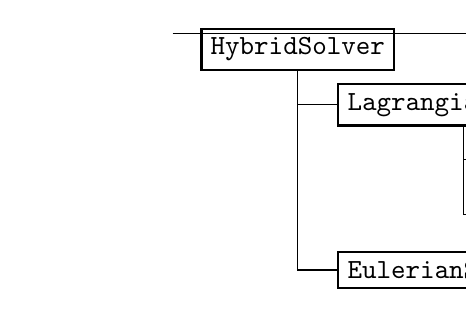
\begin{tikzpicture}[%
  grow via three points={one child at (0.5,-0.7) and
  two children at (0.5,-0.7) and (0.5,-1.4)},
  edge from parent path={(\tikzparentnode.south) |- (\tikzchildnode.west)}]
  \node {\texttt{HybridSolver}}
    child { node {\texttt{LagrangianSolver}}
    	child {node {\texttt{Blobs}}}
    	child {node [selected] {\texttt{Panels}}}  	
    }
    child [missing] {}				
    child [missing] {}				
    child { node {\texttt{EulerianSolver}}};
    %child { node [selected] {tex}
    %  child { node {generic}}
    %  child { node [optional] {latex}}
    %  child { node {plain}}
    %}
    %child [missing] {}
    %child { node {texdoc}};
\end{tikzpicture}
\end{figure}


\subsection*{Class structure:}
\begin{figure}[h]
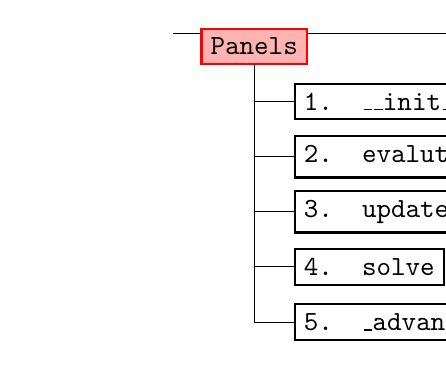
\begin{tikzpicture}[%
  grow via three points={one child at (0.5,-0.7) and
  two children at (0.5,-0.7) and (0.5,-1.4)},
  edge from parent path={(\tikzparentnode.south) |- (\tikzchildnode.west)}]
  \node [selected] {\texttt{Panels}}
    child { node {\texttt{1. \_\_init\_\_}}}
    child { node {\texttt{2. evaluteVelocity}}}                    
    child { node {\texttt{3. updateBody}}}                    
    child { node {\texttt{4. solve}}}                                        
    child { node {\texttt{5. \_advanceTime}}};
\end{tikzpicture}
\end{figure}


\subsection*{Attributes:}
\begingroup
\footnotesize
\begin{longtable}{|l|p{11cm}|}
	\hline
	\textbf{Attributes} & \textbf{Description}\\
	\toprule
    \texttt{A} 		& The inter-induction matrix $\mathbf{A}$, the LHS of the problem. \\ \hline
    \texttt{cmGlobal} & The global position vector for each of the $\mathbf{N}$
                       body, refining the position of the local panel $(0,0)$ in the
                       global coordinate system. \\\hline
    \texttt{deltaT} & The simulation time step size $\Delta T$\\ \hline
    \texttt{geometryKeys} & The dictionary containing all the parameters of the geometry. Contains: \texttt{xPanel} (the $x$ coordinate of the $\mathbf{M}$ panel corners.), \texttt{yPanel} (The $y$ coordinate of the $\mathbf{M}$ panel corners), \texttt{cmGlobal}, \texttt{thetaLocal}, \texttt{dPanel} (The off-set of the panel collocation point from the panel mid-point).  \\ \hline
    \texttt{nBodies} & The number of panel bodies.\\\hline
    \texttt{norm} & The $x$, $y$ normal vector of each panel.\\\hline
    \texttt{normCat} & The global concatenated $x$, $y$ component of the panel normal vector at each collocation points.\\          \hline
    \texttt{nPanels} & The number of panels in each body/geometry. \\ \hline
    \texttt{nPanelsTotal} & The total number of panels.\\    \hline      
    \texttt{panelKernel} & A string defining panel kernel type. \\\hline          
    \texttt{problemType} & A string defining the panel problem is of a \texttt{moving} type or of a \texttt{fixed} type.\\ \hline
    \texttt{solverCompParams} & The dictionary containing solver computation parameters.\\          \hline
	\texttt{sPanel} & The vortex sheet strengths $\gamma$ of $\mathbf{M}$ panels. \\          \hline
	\texttt{t} & The current time $t$ of the simulation.\\          \hline
	\texttt{tang} & The $x$, $y$ tangent vector of each panel.\\          \hline
	\texttt{tangCat} & The global concatenated $x$, $y$ component of the panel
	                  normal vector at each collocation points.\\          \hline
	\texttt{thetaLocal} & The local rotation angle $\theta$ w.r.t to the local
	                     coordinate system. The rotational will be performed around
	                     the local reference point $(0,0)$, i.e around the global center of rotation point \texttt{cmGlobal}.\\          \hline
	\texttt{tStep} & The current step of the simulation.\\          \hline
	\texttt{velCompParams} & A dictionary containing the velocity computation parameters, method and hardware.\\          \hline
	\texttt{xyCPGlobal} & The global $x$, $y$ coordinate of the panel collocation
	                     points.\\ \hline
	\texttt{xyCPGlobalCat} & The global concatenated $x$, $y$ coordinate of the
	                        panel collocation points.\\          \hline
	\texttt{xyPanelGlobal} & The global $x$, $y$ coordinate of the panel bodies.\\          \hline
	\texttt{xyPanelGlobalCat} & The global concatenated $x$, $y$ coordinate of the
	                           panel bodies.\\          \hline
	\texttt{xyPanelLocal} & The local $x$, $y$ coordinate of the panel bodies.\\          \hline
                       
    \caption{Attributes of \texttt{Panels} class and their description.}
    \label{tab:attributesPanels}
\end{longtable}
\endgroup


\subsection*{\texttt{\_\_init\_\_}}
	\begin{tabular}{l|lp{7cm}}
		\multicolumn{2}{l}{\textbf{Input Parameters}} & \\ \hline
		\textit{File Name} & \multicolumn{2}{l}{Containing all the parameters to re-initalize the class.} \\ \hline
		\multirow{2}{*}{\textit{Parameters}} & Panel coordinates &: \{\texttt{xCP, yCP, xPanel, yPanel, cmGlobal, thetaLocal}\}\\ \cline{2-3}
		& External velocity &: \texttt{externVel} \\ \cline{2-3}
	\end{tabular}
	\paragraph{Description:} Initialize the \texttt{panels} class with the given input parameters. In the case of a multibody problem, a list of panel coordinates can be given and internally it takes care of the inter-coupling.\\
	\\
	\begin{tabular}{lp{10cm}}
				\textit{Panel coordinates} & \\ \hline
				\texttt{xCP,yCP} &:  the local $x,y$-coordinates of the panel collocation points.\\ 
				\texttt{xPanel,yPanel} &: the local coordinate of the panel edges. \textit{Note}: Should have a closed loop (end with initial point coordinates).\\ 
				\texttt{cmGlobal} &:  the position of reference points of a given panel body.\\
				\texttt{thetaLocal} &:  the rotational angles of the panel body axes w.r.t to the global $x$-axis.\\
	\end{tabular}\\ 
    \\ \\
	\begin{tabular}{lp{10cm}}
				\textit{External velocity} & \\ \hline
				\texttt{externVel} &:  Reference to an external velocity \textbf{function} acting of the panels. For the panel case, the external velocity will the induced velocity of the blobs + freestream \texttt{vortexBlob.evaluateVelocity}.\\
	\end{tabular}\\
	
		\begin{tabular}{lp{10cm}}
			\textbf{Input parameters} &: \texttt{xCP,yCP}\\ 
			\textbf{Assigns} &: \texttt{-}\\ 			
			\textbf{Returns} &: \texttt{vxCP,vyCP}\\ 					
		\end{tabular}\\


\newpage
%%%%%%%%%%%%%%%%%%%%%%%%%%%%%%%%%%%%%%%%%%%%%%%%%%%%%%%%%%%%%%%%%%%%%%%%%%%%%%%%%%%%%%%%%%%%%%%%%%%%%%%%%%%%%%%%%%%%%%%%%%%%%%%%%%
%%%%%%%%%%%%%%%%%%%%%%%%%%%%%%%%%%%%%%%%%%%%%%%%%%%%%%%%%%%%%%%%%%%%%%%%%%%%%%%%%%%%%%%%%%%%%%%%%%%%%%%%%%%%%%%%%%%%%%%%%%%%%%%%%%

\section*{\texttt{LagrangianSolver} Class}
The main structure of the \texttt{Blobs} + \texttt{Panels} (LagrangianSolver) class. This class contains all the function related to the calculations of panel with vortex blobs.

\begin{figure}[h]
\centering
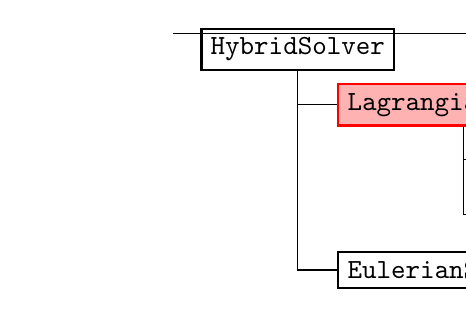
\begin{tikzpicture}[%
  grow via three points={one child at (0.5,-0.7) and
  two children at (0.5,-0.7) and (0.5,-1.4)},
  edge from parent path={(\tikzparentnode.south) |- (\tikzchildnode.west)}]
  \node {\texttt{HybridSolver}}
    child { node [selected] {\texttt{LagrangianSolver}}
    	child {node {\texttt{Blobs}}}
    	child {node {\texttt{Panels}}}  	
    }
    child [missing] {}				
    child [missing] {}				
    child { node {\texttt{EulerianSolver}}};
    %child { node [selected] {tex}
    %  child { node {generic}}
    %  child { node [optional] {latex}}
    %  child { node {plain}}
    %}
    %child [missing] {}
    %child { node {texdoc}};
\end{tikzpicture}
\end{figure}

\subsection*{Class structure:}
\begin{figure}[h]
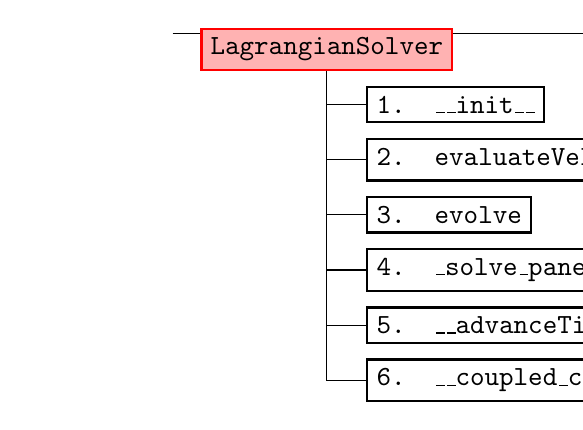
\begin{tikzpicture}[%
  grow via three points={one child at (0.5,-0.7) and
  two children at (0.5,-0.7) and (0.5,-1.4)},
  edge from parent path={(\tikzparentnode.south) |- (\tikzchildnode.west)}]
  \node [selected] {\texttt{LagrangianSolver}}
    child { node {\texttt{1. \_\_init\_\_}}}
    child { node {\texttt{2. evaluateVelocity}}}
    child { node {\texttt{3. evolve}}}
    child { node {\texttt{4. \_solve\_panelStrength}}}                        
    child { node {\texttt{5. \_\_advanceTime}}}                        
    child { node {\texttt{6. \_\_coupled\_convection}}};                       

\end{tikzpicture}
\end{figure}

\subsection*{Attributes:}
\begingroup
\footnotesize
\begin{longtable}{|l|p{12cm}|}
	\hline
	\textbf{Attributes} & \textbf{Description}\\
	\toprule
    \texttt{deltaT}     & The inter-induction matrix $\mathbf{A}$, the LHS of the problem. \\ \hline
    \texttt{gTotal}     & The total circulation of the Lagrangian domain. \\ \hline    
	\texttt{t} & The current time $t$ of the simulation.\\          \hline
	\texttt{tStep} & The current step of the simulation.\\          \hline
	\texttt{vInf} & The $x$, $y$ component of the free-stream velocity.\\          \hline	
	\texttt{Blobs} & The vortex blobs class \texttt{Blobs}.\\          \hline	
	\texttt{Panels} & The vortex panels class \texttt{Panels}.\\          \hline			
                      
    \caption{Attributes of \texttt{LagrangianSolver} class and their description.}
    \label{tab:attributesLagrangianSolver}
\end{longtable}
\endgroup


\subsection*{\texttt{\_\_init\_\_}}
	\begin{tabular}{l|lp{7cm}}
		\multicolumn{2}{l}{\textbf{Input Parameters}} & \\ \hline
		\textit{File Name} & \multicolumn{2}{l}{Containing all the parameters to re-initalize the class.} \\ \hline
		\multirow{2}{*}{\textit{Parameters}} & \texttt{vortexBlobs} &: \{\texttt{vortexBlobs}\} class. \\ \cline{2-3}
		& \texttt{panels} &: \texttt{panels} class. \\ \cline{2-3}
	\end{tabular}
	\paragraph{Description:} Initialize the \texttt{vortexMethod} class using \textbf{vortexBlob}+\textbf{panelMethod} \\ classes.
	\paragraph{Input parameters:}
	\begin{list}{\quad}{}
	\item \texttt{Blobs}: vortex particle class
	\item \texttt{Panels}: panel method class				
	\end{list}


\newpage
%%%%%%%%%%%%%%%%%%%%%%%%%%%%%%%%%%%%%%%%%%%%%%%%%%%%%%%%%%%%%%%%%%%%%%%%%%%%%%%%%%%%%%%%%%%%%%%%%%%%%%%%%%%%%%%%%%%%%%%%%%%%%%%%%%
%%%%%%%%%%%%%%%%%%%%%%%%%%%%%%%%%%%%%%%%%%%%%%%%%%%%%%%%%%%%%%%%%%%%%%%%%%%%%%%%%%%%%%%%%%%%%%%%%%%%%%%%%%%%%%%%%%%%%%%%%%%%%%%%%%

\section*{\texttt{EulerianSolver}}
The main structure for the Navier-stokes class \texttt{EulerianSolver}. This class contains all the functions related to computation of the Navier-stokes problem. Below is set of functions that acts as the interface to the class.

\begin{figure}[h]
\centering
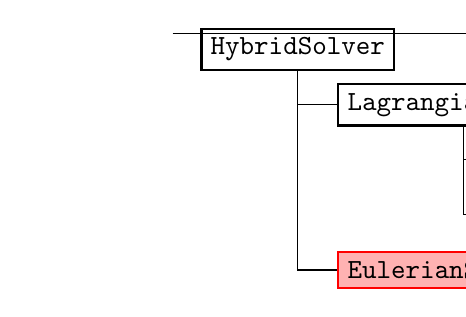
\begin{tikzpicture}[%
  grow via three points={one child at (0.5,-0.7) and
  two children at (0.5,-0.7) and (0.5,-1.4)},
  edge from parent path={(\tikzparentnode.south) |- (\tikzchildnode.west)}]
  \node {\texttt{HybridSolver}}
    child { node {\texttt{LagrangianSolver}}
    	child {node {\texttt{Blobs}}}
    	child {node {\texttt{Panels}}}  	
    }
    child [missing] {}				
    child [missing] {}				
    child { node [selected] {\texttt{EulerianSolver}}};
    %child { node [selected] {tex}
    %  child { node {generic}}
    %  child { node [optional] {latex}}
    %  child { node {plain}}
    %}
    %child [missing] {}
    %child { node {texdoc}};
\end{tikzpicture}
\end{figure}



\subsection*{Class structure:}
\begin{figure}[h]
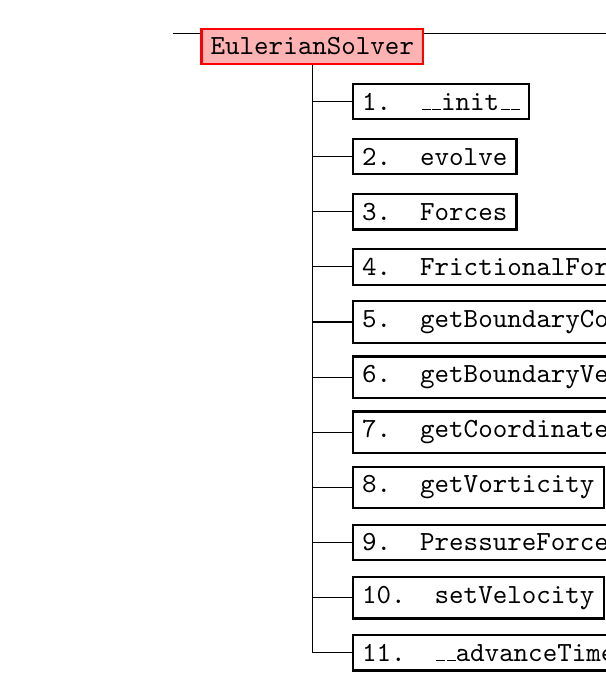
\begin{tikzpicture}[%
  grow via three points={one child at (0.5,-0.7) and
  two children at (0.5,-0.7) and (0.5,-1.4)},
  edge from parent path={(\tikzparentnode.south) |- (\tikzchildnode.west)}]
  \node [selected] {\texttt{EulerianSolver}}
    child { node {\texttt{1. \_\_init\_\_}}}
    child { node {\texttt{2. evolve}}}
    child { node {\texttt{3. Forces}}}
    child { node {\texttt{4. FrictionalForces}}}
    child { node {\texttt{5. getBoundaryCoordinates}}}                            
    child { node {\texttt{6. getBoundaryVelocity}}}                    
    child {node  {\texttt{7. getCoordinates}}}            
    child { node {\texttt{8. getVorticity}}}                                   
    child { node {\texttt{9. PressureForces}}}
    child { node {\texttt{10. setVelocity}}}
    child { node {\texttt{11. \_\_advanceTime}}};
\end{tikzpicture}
\end{figure}


\subsection*{Attributes:}
\begingroup
\footnotesize
\begin{longtable}{|l|p{11cm}|}
	\hline
	\textbf{Attributes} & \textbf{Description}\\
	\toprule
    \texttt{deltaT} 		& The time step size $\Delta t$. \\ \hline
    \texttt{deltaTMax} 		& The maximum allowable time step size $\max\{\Delta t\}$.\\ \hline
    \texttt{cfl} 			& The Courant–Friedrichs–Lewy condition stability number CFL. \\ \hline        
    \texttt{cmGlobal} 		& The $x$, $y$ position of the mesh local reference point $(0,0)$ in the global coordinates. \\ \hline        
    \texttt{hMin} 			& The minimum mesh cell size. \\ \hline        
    \texttt{nu} 			& The fluid kinematic viscosity $\nu$.  \\ \hline        
    \texttt{probeGridMesh} 	& The \textit{local} $x$, $y$ coordinates of the probe grid mesh. \\ \hline            
    \texttt{probeGridParams}& The dictionary containing all the parameters of the probe grid for extracting the vorticity data. \\ \hline            
    \texttt{solverParams} 	& The dictionary file containing all the solver parameters.  \\ \hline                
    \texttt{t} 				& The current time of the simulation. \\ \hline                    
    \texttt{thetaLocal} 	& The local rotational angle $\theta$ of the mesh domain. Therefore, the rotation will be done about local reference  point $(0,0)$, i.e \texttt{cmGlobal} in the global coordinate system.\\ \hline                            
    \texttt{tStep} 			& The current step of the simulation. \\ \hline                    
    \texttt{uMax} 			& The maximum fluid velocity $\max\{\mathbf{u}\}$. \\ \hline
    
    \caption{Attributes of \texttt{EulerianSolver} class and their description.}
    \label{tab:attributeEulerian}
\end{longtable}
\endgroup


\subsection*{\texttt{\_\_init\_\_}}
	\paragraph{Description:} Initialize the \texttt{navierStokes} class either using a \texttt{fileName} containing all the necessary parameter for initialization or by explicitly inputing the parameters.\\

	\begin{tabular}{l|lp{7cm}}
		\multicolumn{2}{l}{\textbf{Input Parameters}} & \\ \hline
		\textit{File Name} & \multicolumn{2}{l}{Containing all the parameters to re-initalize the class.} \\ \hline
		\multicolumn{3}{c}{-- or --} \\ \hline
		\multirow{5}{*}{\textit{Parameters}} & Mesh data &: \texttt{mesh, boundaryDomains}\\ \cline{2-3}
		& Geometry position &: \texttt{cmGlobal, thetaLocal} \\ \cline{2-3}
		& Fluid parameters &: \texttt{uMax, nu}\\ \cline{2-3}
		& Solver options &: \texttt{cfl}\\ \cline{2-3}
		& Probe grid parameters &: \texttt{x0, y0, Lx, Ly, hx, hy}\\ \cline{2-3}

	\end{tabular}\\
	\subsubsection*{Description of the parameters:}
	
	\begin{tabular}{lp{10cm}}
				\textit{Mesh data} & \\ \hline
				\texttt{mesh} &: the mesh data file.\\ 
				\texttt{boundaryDomains} &: the boundary mesh domain data file.\\ 			
	\end{tabular}\\ 
    \\ \\
	\begin{tabular}{lp{10cm}}
				\textit{Geometry position} & \\ \hline
				\texttt{cmGlobal} &: the $x,y$ position of the geometry in global coordinates.\\ 
				\texttt{thetaGlobal} &: the rotation angle (in $rad$) of the geometry in global coordinate system.\\ 			
	\end{tabular}\\
    \\ \\
	\begin{tabular}{lp{10cm}}
				\textit{Fluid parameters} & \\ \hline
				\texttt{uMax} &: the maximum fluid velocity $U_{max}$. Used to determine the maximum time step size $\Delta t_{max}$.\\ 
				\texttt{nu} &: the fluid kinematic viscosity $\nu$, for incompressible navier-stokes problem.\\ 			
	\end{tabular}\\	
    \\ \\
	\begin{tabular}{lp{10cm}}
				\textit{Solver options} & \\ \hline
				\texttt{cfl} &: the $CFL$ stability parameter. If explicit time marching scheme, $CFL<1$.\\ 		
	\end{tabular}\\	
    \\ \\
	\begin{tabular}{lp{10cm}}
				\textit{Probe grid parameters} & \\ \hline
				\texttt{x0,y0} &: the $x,y$ coordinate of the origin of the probe grid.\\ 
				\texttt{Lx,Ly} &: the $x,y$ size (width and height) of the probing grid.\\ 			
				\texttt{hx,hy} &: the $x,y$ spacing of the probe grid cell.\\ 							
	\end{tabular}\\	


\newpage
%%%%%%%%%%%%%%%%%%%%%%%%%%%%%%%%%%%%%%%%%%%%%%%%%%%%%%%%%%%%%%%%%%%%%%%%%%%%%%%%%%%%%%%%%%%%%%%%%%%%%%%%%%%%%%%%%%%%%%%%%%%%%%%%%%
%%%%%%%%%%%%%%%%%%%%%%%%%%%%%%%%%%%%%%%%%%%%%%%%%%%%%%%%%%%%%%%%%%%%%%%%%%%%%%%%%%%%%%%%%%%%%%%%%%%%%%%%%%%%%%%%%%%%%%%%%%%%%%%%%%


\section*{\texttt{HybridSolver} Class}
The main structure for the hybrid class \texttt{HybridSolver}. This class contains all the functions related to computation of the hybrid problem.

\begin{figure}[h]
\centering
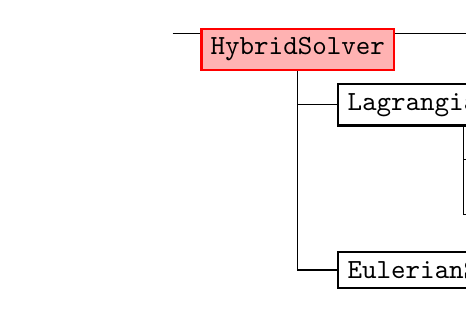
\begin{tikzpicture}[%
  grow via three points={one child at (0.5,-0.7) and
  two children at (0.5,-0.7) and (0.5,-1.4)},
  edge from parent path={(\tikzparentnode.south) |- (\tikzchildnode.west)}]
  \node [selected] {\texttt{HybridSolver}}
    child { node {\texttt{LagrangianSolver}}
    	child {node {\texttt{Blobs}}}
    	child {node {\texttt{Panels}}}  	
    }
    child [missing] {}				
    child [missing] {}				
    child { node {\texttt{EulerianSolver}}};
    %child { node [selected] {tex}
    %  child { node {generic}}
    %  child { node [optional] {latex}}
    %  child { node {plain}}
    %}
    %child [missing] {}
    %child { node {texdoc}};
\end{tikzpicture}
\end{figure}

\subsection*{Class structure:}
\begin{figure}[h]
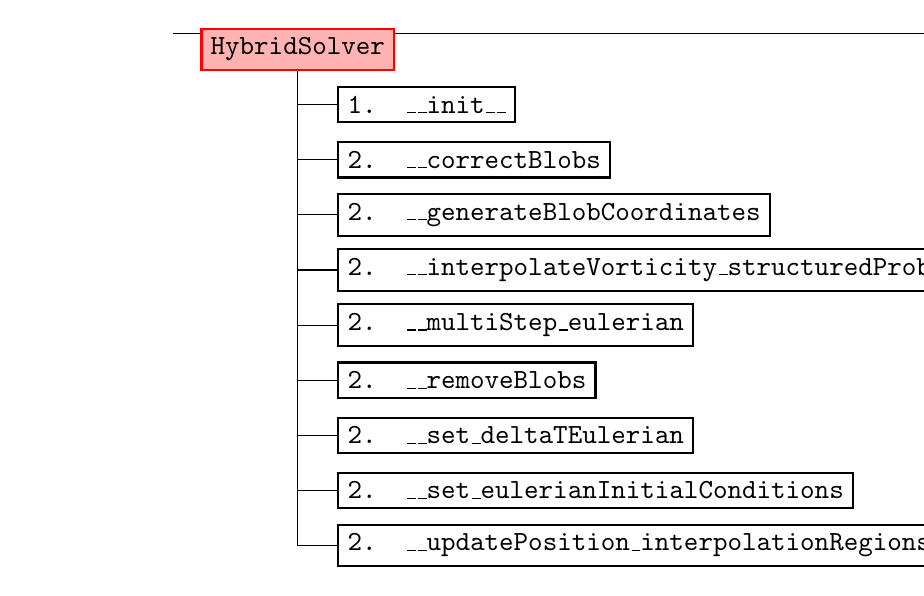
\begin{tikzpicture}[%
  grow via three points={one child at (0.5,-0.7) and
  two children at (0.5,-0.7) and (0.5,-1.4)},
  edge from parent path={(\tikzparentnode.south) |- (\tikzchildnode.west)}]
  \node [selected] {\texttt{HybridSolver}}
    child { node {\texttt{1. \_\_init\_\_}}}
    child { node {\texttt{2. \_\_correctBlobs}}}
    child { node {\texttt{2. \_\_generateBlobCoordinates}}}
    child { node {\texttt{2. \_\_interpolateVorticity\_structuredProbes\_manual}}}
    child { node {\texttt{2. \_\_multiStep\_eulerian}}}
    child { node {\texttt{2. \_\_removeBlobs}}}
    child { node {\texttt{2. \_\_set\_deltaTEulerian}}}    
    child { node {\texttt{2. \_\_set\_eulerianInitialConditions}}}        
    child { node {\texttt{2. \_\_updatePosition\_interpolationRegions}}};
\end{tikzpicture}
\end{figure}


\subsection*{Attributes:}
\begingroup
\footnotesize
\begin{longtable}{|l|p{10cm}|}
	\hline
	\textbf{Attributes} & \textbf{Description}\\
	\toprule
    \texttt{deltaTEulerian} 		& The time step size of the Eulerian sub-domain $\Delta t_E$. \\ \hline
    \texttt{deltaTLagrangian} 		& The time step size of the Lagrangian sub-domain $\Delta t_L$.\\ \hline
	\texttt{nu} 			& The fluid kinematic viscosity $\nu$.  \\ \hline        
    \texttt{t} 				& The current time $t$ of the simulation. \\ \hline                    
    \texttt{tStep} 			& The current step of the simulation. \\ \hline                    
    \texttt{vInf} 			& The $x$, $y$ component of the free-stream velocity. \\ \hline
    \texttt{interpolationRegion} & The dictionary containing the \texttt{surfacePolygon} and \texttt{boundaryPolygon} defining the boundaries of the interpolation region for each Eulerian sub-domains. The geometry is identified by the keys of the Eulerian sub-domain found in \texttt{multiEulerian}. The coordinates are defined in local coordinate system of the Eulerian grid and will be transformed (rotated + moved) during the evolution step. \\ \hline
    \texttt{lagrangian} 	& The Lagrangian solver class contains all the parameters related to simulation the flow in lagrangian sub-domain. \\ \hline
    \texttt{multiEulerian} 	& The \texttt{multiEulerian} is solver class containing all the Eulerian sub-domains of the hybrid problem. \\ \hline
    
    \caption{Attributes of \texttt{HybridSolver} class and their description.}
    \label{tab:attributeHybrid}
\end{longtable}
\endgroup


\subsection*{\texttt{\_\_init\_\_}}
	\begin{tabular}{l|lp{7cm}}
		\multicolumn{2}{l}{\textbf{Input Parameters}} & \\ \hline
		\textit{File Name} & \multicolumn{2}{l}{Containing all the parameters to re-initalize the class.} \\ \hline
		\multirow{4}{*}{\textit{Parameters}} & \texttt{vortexMethod} &: \{\texttt{vortexMethod}\} class.\\ \cline{2-3}
		& \texttt{navierStokes} &: \texttt{navierStokes} class. \\ \cline{2-3}
		& Interpolation region &: \texttt{xPolygon, yPolygon}\\ \cline{2-3}
		& Motion functions &: \texttt{T, cmGlobal, thetaGlobal, cmDotGlobal, thetaDotGlobal}\\ \cline{2-3}
	\end{tabular}\\
	
	\paragraph{Description:} Initialize the \texttt{hybrid} class using \texttt{LagrangianSolver} + \texttt{EulerianSolver} classes.
	\paragraph{Input parameters:}
	\begin{list}{\quad}{}
	\item \texttt{LagrangianSolver}: The vortex method containing \texttt{Blobs} and \textbf{Panels} classes which can already handle the multi-body problem.
	\item \texttt{EulerianSolver}: The Navier-Stokes grid solver class (if multiple: list of \\ \texttt{EulerianSolver} classes). The number of navier-stokes class has to be same as the number of vortex panels.
	\item \textbf{Interpolation Region}: the Navier-Stokes class (if multiple: list of \\ \texttt{EulerianSolver} classes). Should be equal to number of Navier-Stokes classes. The interpolation region should be defined as list of $x,y$ coordinates of the polygon of the interpolation region.
	\item \textbf{Motion function}: the function describing the motion of all the geometries in the hybrid class.
	\end{list}
	
	\begin{tabular}{lp{10cm}}
		\textit{Interpolation Regions} & \\ \hline
		\texttt{xPolygon,yPolygon}: & the new $x,y$ coordinate of the polygons description the interpolation region. The polygon should have a closed loop (end  with starting coordinates) before continuing to the next polygon. In the case of multiple polygons, a list of \texttt{xPolygon,yPolygon} should be given and should be as many as the number of navier-stokes domain.\\ 
	\end{tabular} \vspace{5 mm}

	\begin{tabular}{lp{10cm}}
		\textit{Motion function} & \\ \hline
		\texttt{T} &: the current time.\\ 
		\texttt{cmGlobal} &: a list of new positions of the geometries in the hybrid problem.\\ 
		\texttt{thetaGlobal} &: a list of new rotational angle of the geometries in the hybrid problem.\\ 		
		\texttt{cmDotGlobal} &: a list of current displacement velocity of the geometries in the hybrid problem.\\ 				
		\texttt{thetaDotGlobal} &: a list of current rotational velocity of the geometries in the hybrid problem.\\ 						
	\end{tabular} \vspace{5 mm}

	\begin{tabular}{lp{10cm}}
		\textbf{Input parameters} &: \texttt{T}\\ 
		\textbf{Assigns} &: \texttt{-}\\ 			
		\textbf{Returns} &: \texttt{cmGlobal,thetaGlobal,cmDotGlobal,thetaDotGlobal}\\ 					
	\end{tabular}



% Include all the documents
%\section{\texttt{vortexBlobs}}
The main structure of the \texttt{vortexBlobs} class. This class contains all the function related to the calculation of the vortex blobs.
\begin{figure}[h]
\centering
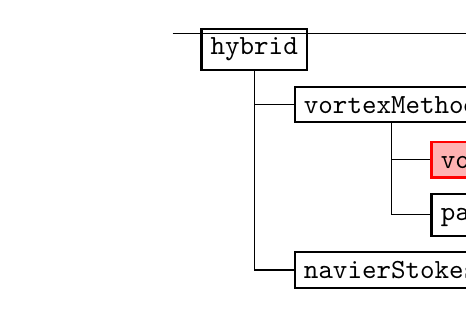
\begin{tikzpicture}[%
  grow via three points={one child at (0.5,-0.7) and
  two children at (0.5,-0.7) and (0.5,-1.4)},
  edge from parent path={(\tikzparentnode.south) |- (\tikzchildnode.west)}]
  \node {\texttt{hybrid}}
    child { node {\texttt{vortexMethod}}
    	child {node [selected] {\texttt{vortexBlobs}}}
    	child {node {\texttt{panels}}}  	
    }
    child [missing] {}				
    child [missing] {}				
    child { node {\texttt{navierStokes}}};
    %child { node [selected] {tex}
    %  child { node {generic}}
    %  child { node [optional] {latex}}
    %  child { node {plain}}
    %}
    %child [missing] {}
    %child { node {texdoc}};
\end{tikzpicture}
\end{figure}

\subsection*{Class structure:}
\begin{figure}[h]
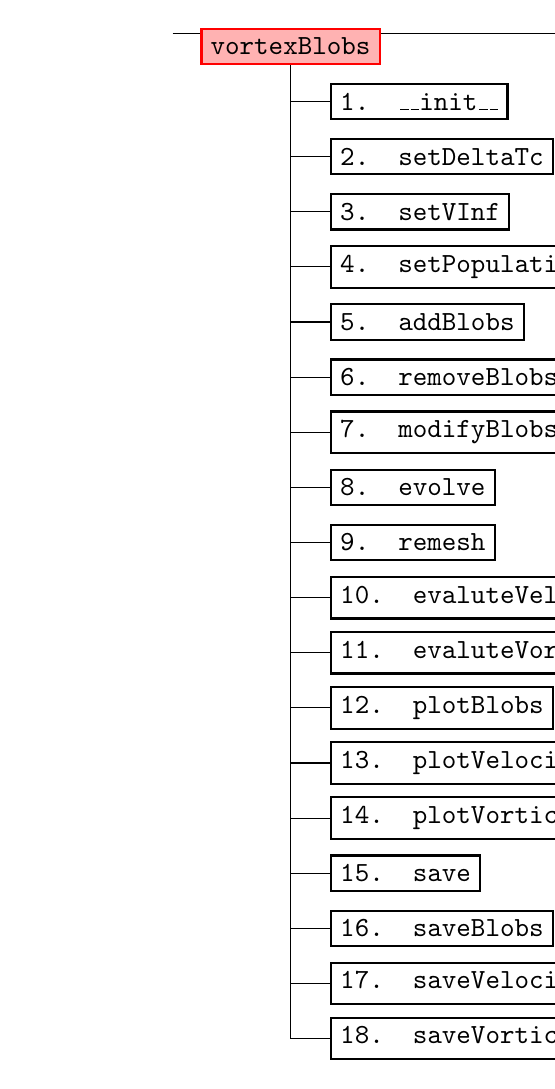
\begin{tikzpicture}[%
  grow via three points={one child at (0.5,-0.7) and
  two children at (0.5,-0.7) and (0.5,-1.4)},
  edge from parent path={(\tikzparentnode.south) |- (\tikzchildnode.west)}]
  \node [selected] {\texttt{vortexBlobs}}
    child { node {\texttt{1. \_\_init\_\_}}}
    child { node {\texttt{2. setDeltaTc}}}
    child { node {\texttt{3. setVInf}}}    
    child { node {\texttt{4. setPopulationControl}}}
    child { node {\texttt{5. addBlobs}}}
    child { node {\texttt{6. removeBlobs}}}    
    child { node {\texttt{7. modifyBlobs}}}    
    child { node {\texttt{8. evolve}}}    
    child { node {\texttt{9. remesh}}}    
    child { node {\texttt{10. evaluteVelocity}}}                    
    child { node {\texttt{11. evaluteVorticity}}}                        
    child { node {\texttt{12. plotBlobs}}}                        
    child { node {\texttt{13. plotVelocity}}}                        
    child { node {\texttt{14. plotVorticity}}}                            
    child { node {\texttt{15. save}}}                        
    child { node {\texttt{16. saveBlobs}}}                                        
    child { node {\texttt{17. saveVelocity}}}                                            
    child { node {\texttt{18. saveVorticity}}};
%    child { node [optional] {19. \texttt{\_generateBlobs}}}
%    child { node [optional] {20. \texttt{\_populationControl}}};        
        %child { node [selected] {tex}
    %  child { node {generic}}
    %  child { node [optional] {latex}}
    %  child { node {plain}}
    %}
    %child { node {texdoc}};
\end{tikzpicture}
\end{figure}

%\subsection*{Structure:}
%\begin{table}[h]
%\begin{tabular}{rl}
%	\texttt{vortexBlobs}: &  \\ \hline
%	-- & \texttt{\_\_init\_\_} \\
%	& \\
%	-- & \texttt{set\_deltaTc} \\ 
%	-- & \texttt{set\_popControlParameters} \\ 
%	-- & \texttt{addBlobs} \\ 
%	-- & \texttt{removeBlobs} \\ 
%	-- & \texttt{modifyBlobs} \\ 
%	-- & \texttt{evolve} \\ 
%	-- & \texttt{remesh} \\ 
%	-- & \texttt{evaluteVelocity} \\ 
%	-- & \texttt{evaluteVorticity} \\ 
%	-- & \texttt{plotBlobs} \\	
%	-- & \texttt{plotVelocity} \\
%	-- & \texttt{plotVorticity} \\
%	-- & \texttt{saveClass} \\ 
%	-- & \texttt{saveBlob} \\ 
%	-- & \texttt{saveVelocity} \\ 	
%	-- & \texttt{saveVorticity} \\ 
%	-- & \texttt{saveBlobPlot} \\ 
%	-- & \texttt{saveVelocityPlot} \\ 	
%	-- & \texttt{saveVorticityPlot} \\ 		
%	& \\
%	-- & \texttt{\_generateParticles} \\ 
%	-- & \texttt{\_popControl} \\
%\end{tabular}
%\end{table}

\newpage



\subsection{\texttt{\_\_init\_\_}}
	\paragraph{Description:} Initialize the \texttt{vortexBlobs} class with either the given input parameters or by a reading a \texttt{file} containing all the necessary parameters.\\
	
	\begin{tabular}{l|lp{7cm}}
		\multicolumn{2}{l}{\textbf{Input Parameters}} & \\ \hline
		\textit{File Name} & \multicolumn{2}{l}{Containing all the parameters to re-initalize the class.} \\ \cline{2-3}
		\multicolumn{3}{c}{--- or ---} \\ \cline{2-3}
		\multirow{4}{*}{\textit{Parameters}} & Vorticity Field &: \{\texttt{xBlob, yBlob, gBlob}\} or \{\texttt{wFunction, xBounds, yBounds}\}\\ \cline{2-3}
		& Blob parameters &: \texttt{overlap, h} \\ \cline{2-3}
		& Time Step parameters &: \texttt{deltaTc, nu, stepRedistribution, integrationMethod, computationMethod}\\ \cline{2-3}
		& Population control parameters &: \texttt{stepPopulationControl, gThreshold}\\ \cline{2-3}
	\end{tabular}\\
	
	\subsubsection*{Descriptions of the parameters:}
	\begin{tabular}{p{3.5cm}p{9cm}p{1cm}}
				\textit{Vorticity field} & & \textit{Default}\\ \hline
				\texttt{xBlob,yBlob} &:  the $x,y$ blob coordinates. & - \\
				\texttt{gBlob} &: the circulation $\Gamma_i$ associated to each of the vortex blobs. & - \\
				& & \\
				\multicolumn{2}{c}{\textit{--- or ---}} & \\
				& & \\
				\texttt{wExactFunction} &: the function that returns the exact value of vorticity $\omega$ at any given $x,y$ coordinates. &\\
				& 	\begin{tabular}{lp{10cm}}
						\textbf{Input parameters} &: \texttt{xEval,yEval}\\ 
						\textbf{Assigns} &: \texttt{-}\\ 			
						\textbf{Returns} &: \texttt{wEval}\\ 					
					\end{tabular} & - \\
				\texttt{xBounds, yBounds} &: the $x,y$ bounds of the domain where the particles was originally distributed. & - \\		 
	\end{tabular}\\
	\\ \\
	%	\begin{tabular}{lp{10cm}}
	%		\textbf{Input parameters} &: \texttt{xEval,yEval}\\ 
	%		\textbf{Assigns} &: \texttt{-}\\ 			
	%		\textbf{Returns} &: \texttt{vortEval}\\ 					
	%	\end{tabular}\\
	\begin{tabular}{p{3.5cm}p{9cm}p{1cm}}
				\multicolumn{2}{l}{\textit{Blob parameters}} & \textit{Default} \\ \hline				
				\texttt{overlap} &: the overlap ratio $h/\sigma$. & 1.0\\
				\texttt{h} &: the size of the cell $h$ associated to the blobs. \textit{Note:} Cells are square. & -\\
	\end{tabular}\\
	\\ \\
	\begin{tabular}{p{3.5cm}p{9cm}p{1cm}}
				\multicolumn{2}{l}{\textit{Time step parameters}} & \textit{Default}\\ \hline
				\texttt{deltaTc} &:  the size of the convective time step $\Delta t_c$. & - \\
				\texttt{nu} &: the fluid kinematic viscosity $\nu$, used to calculate the diffusion coefficient $c^2$ and diffusion time step size $\Delta T_d$.& - \\
				\texttt{stepRedistribution} &: the redistribution step frequency. & 1 \\
				\texttt{integrationMethod} &: the time integration method (\texttt{FE}: Forward euler , \texttt{RK4}: $4^{th}$ order Runge-Kutta). & RK4 \\
				\texttt{computationMethod} &: the calculation method to evolve the blobs, (\texttt{Direct}: Direct Method, \texttt{FMM}: Fast-Multipole Method) using (\texttt{CPU}, \texttt{GPU}). & \{FMM, GPU\}.\\
	\end{tabular}\\ 
    \\ \\ 
	\begin{tabular}{p{3.5cm}p{9cm}p{1cm}}
				\multicolumn{2}{l}{\textit{Population control parameters}} & \textit{Default} \\ \hline
				\texttt{stepPopulationControl} &: population control step frequency & 1.\\
				\texttt{gThreshold} &: the tuple with minimum \textbf{and} maximum value of the circulation $\Gamma_{min}$. & - \\
	\end{tabular}\\ 
    \\ \\  
	\begin{tabular}{p{3.5cm}p{9cm}p{1cm}}
				\multicolumn{2}{l}{\textit{Free stream velocity}} & \textit{Default}\\ \hline
				\texttt{vInf} &: The free-stream velocity function, returning the velocity action on the vortex blobs. & -\\		
				&		\begin{tabular}{lp{10cm}}
							\textbf{Input parameters} &: \texttt{t}\\ 
							\textbf{Assigns} &: \texttt{-}\\ 			
							\textbf{Returns} &: \texttt{vx,vy}\\ 					
						\end{tabular} & - \\
				
	\end{tabular}\\


\subsection{\texttt{setDeltaTc}}
	\paragraph{Description:} Function change the convective time step size $\Delta t_c$.\\
	
	 \begin{tabular}{p{3.5cm}p{10cm}p{1cm}}
				\multicolumn{2}{l}{\textit{Parameters}} & \textit{Default} \\ \hline
		   		\texttt{deltaTc} &: the new convection time step size $\Delta t_c$. & - \\
		\end{tabular} \vspace{5 mm}\\
	\\		
	\begin{tabular}{lp{10cm}}
		\textbf{Input parameters} &: \texttt{deltaTcNew}\\
		\textbf{Assigns} &:  \texttt{deltaTc}\\
		\textbf{Returns} &: \texttt{-}\\
	\end{tabular}

\subsection{\texttt{setPopulationControl}}
	\paragraph{Description:} function to modify the population control parameters.\\
	
	 \begin{tabular}{lp{10cm}}
				\textit{Parameters} & \\ \hline
		   		\texttt{gThresholdNew} &: the minimum and maximum circulation of the blobs, $\Gamma_{min}$\\
		   		\texttt{stepPopulationControlNew} &: the step number (frequency) of the population control.\\
		\end{tabular} \vspace{5 mm}\\
	\\		
	\begin{tabular}{lp{10cm}}
		\textbf{Input parameters} &: \texttt{gThresholdNew, stepPopulationControlNew}\\
		\textbf{Assigns} &:  \texttt{gThreshold, stepPopulationControl}\\
		\textbf{Returns} &: \texttt{-}\\
	\end{tabular}

		
\subsection{\texttt{addBlobs}}
	\paragraph{Description:} adds vortex particles by appending to the current set of particles.\\
	
	 \begin{tabular}{lp{10cm}}
				\textit{Parameters} & \\ \hline
		   		\texttt{xBlobNew,yBlobNew,gBlobNew} &: the coordinates and the strength of the new set of particles.\\
		\end{tabular} \vspace{5 mm}\\
	\\		
	\begin{tabular}{lp{10cm}}
		\textbf{Input parameters} &: \texttt{xBlobNew,yBlobNew,gBlobNew}\\
		\textbf{Assigns} &: \texttt{xBlob,yBlob,gBlob}\\
		\textbf{Returns} &: \texttt{-}\\
	\end{tabular}


\subsection{\texttt{removeBlobs}}
	\paragraph{Description:} removes vortex particles from the current set of particles. Using, the particle index, the associated $x,y$ and $\Gamma_i$ will be removed.\\
	
	 \begin{tabular}{lp{10cm}}
				\textit{Parameters} & \\ \hline
		   		\texttt{iBlob} &: the list of blob indices that is to be removed.\\
		\end{tabular} \vspace{5 mm}\\
	\\		
	\begin{tabular}{lp{10cm}}
		\textbf{Input parameters} &: \texttt{iBlob}\\
		\textbf{Assigns} &: \texttt{xBlob,yBlob,gBlob}\\
		\textbf{Returns} &: \texttt{-}\\
	\end{tabular}
	
	
\subsection{\texttt{modifyBlobs}}
	\paragraph{Description:} Replace the vortex particle strengths with the new strength.\\
	
	 \begin{tabular}{lp{10cm}}
				\textit{Parameters} & \\ \hline
		   		\texttt{iBlob} &: the list of blob indices that is to be modified.\\
		   		\texttt{gBlobNew} &: the new strength of the blobs.\\		   		
		\end{tabular} \vspace{5 mm}\\
	\\		
	\begin{tabular}{lp{10cm}}
		\textbf{Input parameters} &: \texttt{iBlob,gBlobNew}\\
		\textbf{Assigns} &: \texttt{gBlob}\\
		\textbf{Returns} &: \texttt{-}\\
	\end{tabular}	

\subsection{\texttt{evolve}}
	\paragraph{Description:} Evolves the vortex blobs according to the \texttt{\_\_init\_\_} definition. The \texttt{evolve} function, knows when (has a counter) to redistribute and perform population control. Depending on the diffusion time step $\Delta t_d$, the evolve function will also perform the diffusion process (modified interpolation).\\
	
	 \begin{tabular}{lp{10cm}}
				\textit{Parameters} & \\ \hline
		   		\texttt{xBlobNew,yBlobNew,gBlobNew} &: the new set of particle after the evolution process.\\
		\end{tabular} \vspace{5 mm}\\
	\\		
	\begin{tabular}{lp{10cm}}
		\textbf{Input parameters} &: \texttt{-}\\
		\textbf{Assigns} &: \texttt{xBlob,yBlob,gBlob}\\	
		\textbf{Returns} &: \texttt{-}\\
	\end{tabular}			


\subsection{\texttt{remesh}}
	\paragraph{Description:}  Function to remesh the particles on to the remeshing grid. When $c=0$, the remeshing will be done without diffusion. If $c>0$, the modified interpolation will perform the diffusion.
	\\
	\\		
	\begin{tabular}{lp{10cm}}
		\textbf{Input parameters} &: \texttt{c}\\ 
		\textbf{Assigns} &: \texttt{xBlob,yBlob,wBlob}\\ 			
		\textbf{Returns} &: \texttt{-}\\ 					
	\end{tabular}


\subsection{\texttt{evaluateVelocity}}
	\paragraph{Description:} Function to evaluate the total induced velocity due to the blobs, and the external velocity at a given target locations.\\
	
	    \begin{tabular}{lp{10cm}}
			\textit{Parameters} & \\ \hline
			 \texttt{xTarget,yTarget} &: the $x,y$ coordinate of the target location, where the total velocity is to be evaluated.\\
			\texttt{vxTarget,vyTarget} &: the $x,y$ induced velocity at the target points in global coordinate system.\\
		\end{tabular} \vspace{5 mm}
	\\		
	\begin{tabular}{lp{10cm}}
		\textbf{Input parameters} &: \texttt{xTarget,yTarget}\\ 
		\textbf{Assigns} &: \texttt{-}\\ 			
		\textbf{Returns} &: \texttt{vxTarget,vyTarget}\\ 					
	\end{tabular}	

\subsection{\texttt{evaluateVorticity}}
	\paragraph{Description:} Function to evaluate the total induced vorticity due to the blobs, and the external velocity at a given target coordinates.\\
	
	    \begin{tabular}{lp{10cm}}
			\textit{Parameters} & \\ \hline
			 \texttt{xTarget,yTarget} &: the $x,y$ coordinate of the target location, where the total velocity is to be evaluated.\\
			\texttt{wTarget} &: the $x,y$ induced vorticity at the target points in global coordinate system.\\
		\end{tabular} \vspace{5 mm}
	\\		
	\begin{tabular}{lp{10cm}}
		\textbf{Input parameters} &: \texttt{xTarget,yTarget}\\ 
		\textbf{Assigns} &: \texttt{-}\\ 			
		\textbf{Returns} &: \texttt{wTarget}\\ 					
	\end{tabular}


		
\subsection{plots \ldots}
	\paragraph{Description:} functions to plot and/or save all the results in a given region. The data should be store for scientific visualization (paraview format)\\
	
		\begin{tabular}{lp{10cm}}
			\textit{Plot variables:} & \\ \hline
			\texttt{plotBlob} &: plot the coordinates and the circulation of the blobs.\\
			\texttt{plotVelocity} &: plot the velocity field.\\ 
			\texttt{plotVorticity} &: plot the vorticity field.\\ 
		\end{tabular} \vspace{5 mm}
		
		\begin{tabular}{lp{10cm}}
			\textit{Parameters:} & \\ \hline
			\texttt{xBounds,yBounds} &: $x,y$ bounds of the grid, where the data is to be evaluated.\\ 
			\texttt{nGrid} &: $x,y$ number of grid points.\\
		\end{tabular} \vspace{5 mm}\\
	\\
	\begin{tabular}{lp{10cm}}
		\textbf{Input parameters} &: \texttt{xBounds,yBounds,nGrid}\\
		\textbf{Assigns} &: \texttt{-}\\ 			
		\textbf{Returns} &: \texttt{figureHandle} or \texttt{.pvd}\\ 					
	\end{tabular}	

\subsection{save data \ldots}
	\paragraph{Description:} functions to save the data. The data file will be in compressed, binary format to store efficiently.\\

		\begin{tabular}{lp{10cm}}
			\textit{Save variables:} & \\ \hline
			\texttt{save} &: all the data of the \texttt{vortexBlob} class is saved. This can be used later to restart the problem, i.e the parameter to init the problem.\\
			\texttt{saveBlobs} &: the function to save the blob data at the current time instant. List of numpy array.\\ 			
			\texttt{saveVelocity} &: save the velocity field of a given region or a given set of points.\\ 
			\texttt{saveVorticity} &: save the vorticity field of the given region or the given set of points.\\ 
		\end{tabular} \vspace{5 mm}
	
		\begin{tabular}{lp{10cm}}
			\textit{Parameters:} & \\ \hline
			\texttt{xBounds,yBounds} &: $x,y$ bounds of the grid, where the data is to be evaluated and saved.\\ 
			\texttt{nGrid} &: $x,y$ number of grid points.\\
			\texttt{xEval,yEval} &: $x,y$ coordinates of the location where the data is to be evaluated and saved.\\ 
		\end{tabular} \vspace{5 mm}\\
	\\
	\begin{tabular}{lp{10cm}}
		\textbf{Input parameters} &: \texttt{xBounds,yBounds,hGrid} or \texttt{xEval,yEval}\\ 
		\textbf{Assigns} &: \texttt{-}\\ 			
		\textbf{Returns} &: \texttt{.npz, .bin or similar}\\ 					
	\end{tabular}



%\subsection{save plots \ldots}
%	\paragraph{Description:} Function to save the plots as scientific visualization format \texttt{.pvd}.\\
%	
%		\begin{tabular}{lp{10cm}}
%			\textit{Save variables:} & \\ \hline
%			\texttt{saveBlobPlot} &: save the particle position and strengths as glyphs.\\
%			\texttt{saveVelocityPlot} &: save the velocity plot of a given region.\\ 
%			\texttt{saveVorticityPlot} &: save the vorticity of a given region.\\ 
%		\end{tabular} \vspace{5 mm}
%		
%		\begin{tabular}{lp{10cm}}
%			\textit{Parameters:} & \\ \hline
%			\texttt{xBounds,yBounds} &: $x,y$ bounds of the grid, where the data is to be evaluated and saved.\\ 
%			\texttt{hGrid} &: $x,y$ spacing of the evaluation grid.\\
%		\end{tabular} \vspace{5 mm}\\
%	\\
%	\begin{tabular}{lp{10cm}}
%		\textbf{Input parameters} &: \texttt{xBounds,yBounds,hGrid}\\
%		\textbf{Assigns} &: \texttt{-}\\ 			
%		\textbf{Returns} &: \texttt{.pvd}\\ 					
%	\end{tabular}
	


%\subsection{\texttt{\_generateParticles}}
%	\paragraph{Description:} \textit{Internal} function to generate/initialize the particles.\\
%	\\
%	\\
%		\begin{tabular}{lp{10cm}}
%			\textbf{Input parameters} &: \texttt{wExactFunction, xBounds, yBounds}\\ 
%			\textbf{Assigns} &: \texttt{xBlob,yBlob,wBlob}\\ 			
%			\textbf{Returns} &: \texttt{-}\\ 					
%		\end{tabular}	
%
%
%\subsection{\texttt{\_popControl}}
%	\paragraph{Description:} \textit{Internal} function to perform population control on the current set of particles.\\
%	\\
%	\\	
%		\begin{tabular}{lp{10cm}}
%			\textbf{Input parameters} &: \texttt{-}\\ 
%			\textbf{Assigns} &: \texttt{xBlob,yBlob,wBlob}\\ 			
%			\textbf{Returns} &: \texttt{-}\\ 					
%		\end{tabular}	
%\section{\texttt{vortexBlobs}}
The main structure of the \texttt{vortexBlobs} class. This class contains all the function related to the calculation of the vortex blobs.
\begin{figure}[h]
\centering
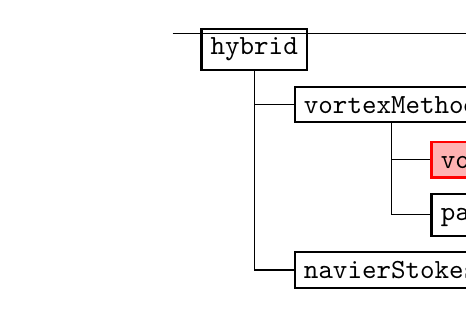
\begin{tikzpicture}[%
  grow via three points={one child at (0.5,-0.7) and
  two children at (0.5,-0.7) and (0.5,-1.4)},
  edge from parent path={(\tikzparentnode.south) |- (\tikzchildnode.west)}]
  \node {\texttt{hybrid}}
    child { node {\texttt{vortexMethod}}
    	child {node [selected] {\texttt{vortexBlobs}}}
    	child {node {\texttt{panels}}}  	
    }
    child [missing] {}				
    child [missing] {}				
    child { node {\texttt{navierStokes}}};
    %child { node [selected] {tex}
    %  child { node {generic}}
    %  child { node [optional] {latex}}
    %  child { node {plain}}
    %}
    %child [missing] {}
    %child { node {texdoc}};
\end{tikzpicture}
\end{figure}

\subsection*{Class structure:}
\begin{figure}[h]
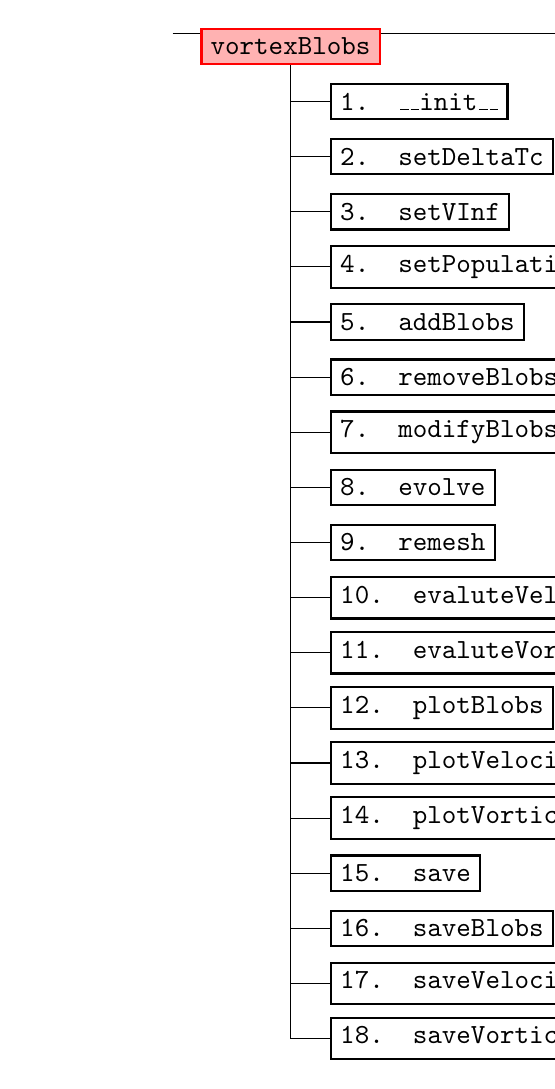
\begin{tikzpicture}[%
  grow via three points={one child at (0.5,-0.7) and
  two children at (0.5,-0.7) and (0.5,-1.4)},
  edge from parent path={(\tikzparentnode.south) |- (\tikzchildnode.west)}]
  \node [selected] {\texttt{vortexBlobs}}
    child { node {\texttt{1. \_\_init\_\_}}}
    child { node {\texttt{2. setDeltaTc}}}
    child { node {\texttt{3. setVInf}}}    
    child { node {\texttt{4. setPopulationControl}}}
    child { node {\texttt{5. addBlobs}}}
    child { node {\texttt{6. removeBlobs}}}    
    child { node {\texttt{7. modifyBlobs}}}    
    child { node {\texttt{8. evolve}}}    
    child { node {\texttt{9. remesh}}}    
    child { node {\texttt{10. evaluteVelocity}}}                    
    child { node {\texttt{11. evaluteVorticity}}}                        
    child { node {\texttt{12. plotBlobs}}}                        
    child { node {\texttt{13. plotVelocity}}}                        
    child { node {\texttt{14. plotVorticity}}}                            
    child { node {\texttt{15. save}}}                        
    child { node {\texttt{16. saveBlobs}}}                                        
    child { node {\texttt{17. saveVelocity}}}                                            
    child { node {\texttt{18. saveVorticity}}};
%    child { node [optional] {19. \texttt{\_generateBlobs}}}
%    child { node [optional] {20. \texttt{\_populationControl}}};        
        %child { node [selected] {tex}
    %  child { node {generic}}
    %  child { node [optional] {latex}}
    %  child { node {plain}}
    %}
    %child { node {texdoc}};
\end{tikzpicture}
\end{figure}

%\subsection*{Structure:}
%\begin{table}[h]
%\begin{tabular}{rl}
%	\texttt{vortexBlobs}: &  \\ \hline
%	-- & \texttt{\_\_init\_\_} \\
%	& \\
%	-- & \texttt{set\_deltaTc} \\ 
%	-- & \texttt{set\_popControlParameters} \\ 
%	-- & \texttt{addBlobs} \\ 
%	-- & \texttt{removeBlobs} \\ 
%	-- & \texttt{modifyBlobs} \\ 
%	-- & \texttt{evolve} \\ 
%	-- & \texttt{remesh} \\ 
%	-- & \texttt{evaluteVelocity} \\ 
%	-- & \texttt{evaluteVorticity} \\ 
%	-- & \texttt{plotBlobs} \\	
%	-- & \texttt{plotVelocity} \\
%	-- & \texttt{plotVorticity} \\
%	-- & \texttt{saveClass} \\ 
%	-- & \texttt{saveBlob} \\ 
%	-- & \texttt{saveVelocity} \\ 	
%	-- & \texttt{saveVorticity} \\ 
%	-- & \texttt{saveBlobPlot} \\ 
%	-- & \texttt{saveVelocityPlot} \\ 	
%	-- & \texttt{saveVorticityPlot} \\ 		
%	& \\
%	-- & \texttt{\_generateParticles} \\ 
%	-- & \texttt{\_popControl} \\
%\end{tabular}
%\end{table}

\newpage



\subsection{\texttt{\_\_init\_\_}}
	\paragraph{Description:} Initialize the \texttt{vortexBlobs} class with either the given input parameters or by a reading a \texttt{file} containing all the necessary parameters.\\
	
	\begin{tabular}{l|lp{7cm}}
		\multicolumn{2}{l}{\textbf{Input Parameters}} & \\ \hline
		\textit{File Name} & \multicolumn{2}{l}{Containing all the parameters to re-initalize the class.} \\ \cline{2-3}
		\multicolumn{3}{c}{--- or ---} \\ \cline{2-3}
		\multirow{4}{*}{\textit{Parameters}} & Vorticity Field &: \{\texttt{xBlob, yBlob, gBlob}\} or \{\texttt{wFunction, xBounds, yBounds}\}\\ \cline{2-3}
		& Blob parameters &: \texttt{overlap, h} \\ \cline{2-3}
		& Time Step parameters &: \texttt{deltaTc, nu, stepRedistribution, integrationMethod, computationMethod}\\ \cline{2-3}
		& Population control parameters &: \texttt{stepPopulationControl, gThreshold}\\ \cline{2-3}
	\end{tabular}\\
	
	\subsubsection*{Descriptions of the parameters:}
	\begin{tabular}{p{3.5cm}p{9cm}p{1cm}}
				\textit{Vorticity field} & & \textit{Default}\\ \hline
				\texttt{xBlob,yBlob} &:  the $x,y$ blob coordinates. & - \\
				\texttt{gBlob} &: the circulation $\Gamma_i$ associated to each of the vortex blobs. & - \\
				& & \\
				\multicolumn{2}{c}{\textit{--- or ---}} & \\
				& & \\
				\texttt{wExactFunction} &: the function that returns the exact value of vorticity $\omega$ at any given $x,y$ coordinates. &\\
				& 	\begin{tabular}{lp{10cm}}
						\textbf{Input parameters} &: \texttt{xEval,yEval}\\ 
						\textbf{Assigns} &: \texttt{-}\\ 			
						\textbf{Returns} &: \texttt{wEval}\\ 					
					\end{tabular} & - \\
				\texttt{xBounds, yBounds} &: the $x,y$ bounds of the domain where the particles was originally distributed. & - \\		 
	\end{tabular}\\
	\\ \\
	%	\begin{tabular}{lp{10cm}}
	%		\textbf{Input parameters} &: \texttt{xEval,yEval}\\ 
	%		\textbf{Assigns} &: \texttt{-}\\ 			
	%		\textbf{Returns} &: \texttt{vortEval}\\ 					
	%	\end{tabular}\\
	\begin{tabular}{p{3.5cm}p{9cm}p{1cm}}
				\multicolumn{2}{l}{\textit{Blob parameters}} & \textit{Default} \\ \hline				
				\texttt{overlap} &: the overlap ratio $h/\sigma$. & 1.0\\
				\texttt{h} &: the size of the cell $h$ associated to the blobs. \textit{Note:} Cells are square. & -\\
	\end{tabular}\\
	\\ \\
	\begin{tabular}{p{3.5cm}p{9cm}p{1cm}}
				\multicolumn{2}{l}{\textit{Time step parameters}} & \textit{Default}\\ \hline
				\texttt{deltaTc} &:  the size of the convective time step $\Delta t_c$. & - \\
				\texttt{nu} &: the fluid kinematic viscosity $\nu$, used to calculate the diffusion coefficient $c^2$ and diffusion time step size $\Delta T_d$.& - \\
				\texttt{stepRedistribution} &: the redistribution step frequency. & 1 \\
				\texttt{integrationMethod} &: the time integration method (\texttt{FE}: Forward euler , \texttt{RK4}: $4^{th}$ order Runge-Kutta). & RK4 \\
				\texttt{computationMethod} &: the calculation method to evolve the blobs, (\texttt{Direct}: Direct Method, \texttt{FMM}: Fast-Multipole Method) using (\texttt{CPU}, \texttt{GPU}). & \{FMM, GPU\}.\\
	\end{tabular}\\ 
    \\ \\ 
	\begin{tabular}{p{3.5cm}p{9cm}p{1cm}}
				\multicolumn{2}{l}{\textit{Population control parameters}} & \textit{Default} \\ \hline
				\texttt{stepPopulationControl} &: population control step frequency & 1.\\
				\texttt{gThreshold} &: the tuple with minimum \textbf{and} maximum value of the circulation $\Gamma_{min}$. & - \\
	\end{tabular}\\ 
    \\ \\  
	\begin{tabular}{p{3.5cm}p{9cm}p{1cm}}
				\multicolumn{2}{l}{\textit{Free stream velocity}} & \textit{Default}\\ \hline
				\texttt{vInf} &: The free-stream velocity function, returning the velocity action on the vortex blobs. & -\\		
				&		\begin{tabular}{lp{10cm}}
							\textbf{Input parameters} &: \texttt{t}\\ 
							\textbf{Assigns} &: \texttt{-}\\ 			
							\textbf{Returns} &: \texttt{vx,vy}\\ 					
						\end{tabular} & - \\
				
	\end{tabular}\\


\subsection{\texttt{setDeltaTc}}
	\paragraph{Description:} Function change the convective time step size $\Delta t_c$.\\
	
	 \begin{tabular}{p{3.5cm}p{10cm}p{1cm}}
				\multicolumn{2}{l}{\textit{Parameters}} & \textit{Default} \\ \hline
		   		\texttt{deltaTc} &: the new convection time step size $\Delta t_c$. & - \\
		\end{tabular} \vspace{5 mm}\\
	\\		
	\begin{tabular}{lp{10cm}}
		\textbf{Input parameters} &: \texttt{deltaTcNew}\\
		\textbf{Assigns} &:  \texttt{deltaTc}\\
		\textbf{Returns} &: \texttt{-}\\
	\end{tabular}

\subsection{\texttt{setPopulationControl}}
	\paragraph{Description:} function to modify the population control parameters.\\
	
	 \begin{tabular}{lp{10cm}}
				\textit{Parameters} & \\ \hline
		   		\texttt{gThresholdNew} &: the minimum and maximum circulation of the blobs, $\Gamma_{min}$\\
		   		\texttt{stepPopulationControlNew} &: the step number (frequency) of the population control.\\
		\end{tabular} \vspace{5 mm}\\
	\\		
	\begin{tabular}{lp{10cm}}
		\textbf{Input parameters} &: \texttt{gThresholdNew, stepPopulationControlNew}\\
		\textbf{Assigns} &:  \texttt{gThreshold, stepPopulationControl}\\
		\textbf{Returns} &: \texttt{-}\\
	\end{tabular}

		
\subsection{\texttt{addBlobs}}
	\paragraph{Description:} adds vortex particles by appending to the current set of particles.\\
	
	 \begin{tabular}{lp{10cm}}
				\textit{Parameters} & \\ \hline
		   		\texttt{xBlobNew,yBlobNew,gBlobNew} &: the coordinates and the strength of the new set of particles.\\
		\end{tabular} \vspace{5 mm}\\
	\\		
	\begin{tabular}{lp{10cm}}
		\textbf{Input parameters} &: \texttt{xBlobNew,yBlobNew,gBlobNew}\\
		\textbf{Assigns} &: \texttt{xBlob,yBlob,gBlob}\\
		\textbf{Returns} &: \texttt{-}\\
	\end{tabular}


\subsection{\texttt{removeBlobs}}
	\paragraph{Description:} removes vortex particles from the current set of particles. Using, the particle index, the associated $x,y$ and $\Gamma_i$ will be removed.\\
	
	 \begin{tabular}{lp{10cm}}
				\textit{Parameters} & \\ \hline
		   		\texttt{iBlob} &: the list of blob indices that is to be removed.\\
		\end{tabular} \vspace{5 mm}\\
	\\		
	\begin{tabular}{lp{10cm}}
		\textbf{Input parameters} &: \texttt{iBlob}\\
		\textbf{Assigns} &: \texttt{xBlob,yBlob,gBlob}\\
		\textbf{Returns} &: \texttt{-}\\
	\end{tabular}
	
	
\subsection{\texttt{modifyBlobs}}
	\paragraph{Description:} Replace the vortex particle strengths with the new strength.\\
	
	 \begin{tabular}{lp{10cm}}
				\textit{Parameters} & \\ \hline
		   		\texttt{iBlob} &: the list of blob indices that is to be modified.\\
		   		\texttt{gBlobNew} &: the new strength of the blobs.\\		   		
		\end{tabular} \vspace{5 mm}\\
	\\		
	\begin{tabular}{lp{10cm}}
		\textbf{Input parameters} &: \texttt{iBlob,gBlobNew}\\
		\textbf{Assigns} &: \texttt{gBlob}\\
		\textbf{Returns} &: \texttt{-}\\
	\end{tabular}	

\subsection{\texttt{evolve}}
	\paragraph{Description:} Evolves the vortex blobs according to the \texttt{\_\_init\_\_} definition. The \texttt{evolve} function, knows when (has a counter) to redistribute and perform population control. Depending on the diffusion time step $\Delta t_d$, the evolve function will also perform the diffusion process (modified interpolation).\\
	
	 \begin{tabular}{lp{10cm}}
				\textit{Parameters} & \\ \hline
		   		\texttt{xBlobNew,yBlobNew,gBlobNew} &: the new set of particle after the evolution process.\\
		\end{tabular} \vspace{5 mm}\\
	\\		
	\begin{tabular}{lp{10cm}}
		\textbf{Input parameters} &: \texttt{-}\\
		\textbf{Assigns} &: \texttt{xBlob,yBlob,gBlob}\\	
		\textbf{Returns} &: \texttt{-}\\
	\end{tabular}			


\subsection{\texttt{remesh}}
	\paragraph{Description:}  Function to remesh the particles on to the remeshing grid. When $c=0$, the remeshing will be done without diffusion. If $c>0$, the modified interpolation will perform the diffusion.
	\\
	\\		
	\begin{tabular}{lp{10cm}}
		\textbf{Input parameters} &: \texttt{c}\\ 
		\textbf{Assigns} &: \texttt{xBlob,yBlob,wBlob}\\ 			
		\textbf{Returns} &: \texttt{-}\\ 					
	\end{tabular}


\subsection{\texttt{evaluateVelocity}}
	\paragraph{Description:} Function to evaluate the total induced velocity due to the blobs, and the external velocity at a given target locations.\\
	
	    \begin{tabular}{lp{10cm}}
			\textit{Parameters} & \\ \hline
			 \texttt{xTarget,yTarget} &: the $x,y$ coordinate of the target location, where the total velocity is to be evaluated.\\
			\texttt{vxTarget,vyTarget} &: the $x,y$ induced velocity at the target points in global coordinate system.\\
		\end{tabular} \vspace{5 mm}
	\\		
	\begin{tabular}{lp{10cm}}
		\textbf{Input parameters} &: \texttt{xTarget,yTarget}\\ 
		\textbf{Assigns} &: \texttt{-}\\ 			
		\textbf{Returns} &: \texttt{vxTarget,vyTarget}\\ 					
	\end{tabular}	

\subsection{\texttt{evaluateVorticity}}
	\paragraph{Description:} Function to evaluate the total induced vorticity due to the blobs, and the external velocity at a given target coordinates.\\
	
	    \begin{tabular}{lp{10cm}}
			\textit{Parameters} & \\ \hline
			 \texttt{xTarget,yTarget} &: the $x,y$ coordinate of the target location, where the total velocity is to be evaluated.\\
			\texttt{wTarget} &: the $x,y$ induced vorticity at the target points in global coordinate system.\\
		\end{tabular} \vspace{5 mm}
	\\		
	\begin{tabular}{lp{10cm}}
		\textbf{Input parameters} &: \texttt{xTarget,yTarget}\\ 
		\textbf{Assigns} &: \texttt{-}\\ 			
		\textbf{Returns} &: \texttt{wTarget}\\ 					
	\end{tabular}


		
\subsection{plots \ldots}
	\paragraph{Description:} functions to plot and/or save all the results in a given region. The data should be store for scientific visualization (paraview format)\\
	
		\begin{tabular}{lp{10cm}}
			\textit{Plot variables:} & \\ \hline
			\texttt{plotBlob} &: plot the coordinates and the circulation of the blobs.\\
			\texttt{plotVelocity} &: plot the velocity field.\\ 
			\texttt{plotVorticity} &: plot the vorticity field.\\ 
		\end{tabular} \vspace{5 mm}
		
		\begin{tabular}{lp{10cm}}
			\textit{Parameters:} & \\ \hline
			\texttt{xBounds,yBounds} &: $x,y$ bounds of the grid, where the data is to be evaluated.\\ 
			\texttt{nGrid} &: $x,y$ number of grid points.\\
		\end{tabular} \vspace{5 mm}\\
	\\
	\begin{tabular}{lp{10cm}}
		\textbf{Input parameters} &: \texttt{xBounds,yBounds,nGrid}\\
		\textbf{Assigns} &: \texttt{-}\\ 			
		\textbf{Returns} &: \texttt{figureHandle} or \texttt{.pvd}\\ 					
	\end{tabular}	

\subsection{save data \ldots}
	\paragraph{Description:} functions to save the data. The data file will be in compressed, binary format to store efficiently.\\

		\begin{tabular}{lp{10cm}}
			\textit{Save variables:} & \\ \hline
			\texttt{save} &: all the data of the \texttt{vortexBlob} class is saved. This can be used later to restart the problem, i.e the parameter to init the problem.\\
			\texttt{saveBlobs} &: the function to save the blob data at the current time instant. List of numpy array.\\ 			
			\texttt{saveVelocity} &: save the velocity field of a given region or a given set of points.\\ 
			\texttt{saveVorticity} &: save the vorticity field of the given region or the given set of points.\\ 
		\end{tabular} \vspace{5 mm}
	
		\begin{tabular}{lp{10cm}}
			\textit{Parameters:} & \\ \hline
			\texttt{xBounds,yBounds} &: $x,y$ bounds of the grid, where the data is to be evaluated and saved.\\ 
			\texttt{nGrid} &: $x,y$ number of grid points.\\
			\texttt{xEval,yEval} &: $x,y$ coordinates of the location where the data is to be evaluated and saved.\\ 
		\end{tabular} \vspace{5 mm}\\
	\\
	\begin{tabular}{lp{10cm}}
		\textbf{Input parameters} &: \texttt{xBounds,yBounds,hGrid} or \texttt{xEval,yEval}\\ 
		\textbf{Assigns} &: \texttt{-}\\ 			
		\textbf{Returns} &: \texttt{.npz, .bin or similar}\\ 					
	\end{tabular}



%\subsection{save plots \ldots}
%	\paragraph{Description:} Function to save the plots as scientific visualization format \texttt{.pvd}.\\
%	
%		\begin{tabular}{lp{10cm}}
%			\textit{Save variables:} & \\ \hline
%			\texttt{saveBlobPlot} &: save the particle position and strengths as glyphs.\\
%			\texttt{saveVelocityPlot} &: save the velocity plot of a given region.\\ 
%			\texttt{saveVorticityPlot} &: save the vorticity of a given region.\\ 
%		\end{tabular} \vspace{5 mm}
%		
%		\begin{tabular}{lp{10cm}}
%			\textit{Parameters:} & \\ \hline
%			\texttt{xBounds,yBounds} &: $x,y$ bounds of the grid, where the data is to be evaluated and saved.\\ 
%			\texttt{hGrid} &: $x,y$ spacing of the evaluation grid.\\
%		\end{tabular} \vspace{5 mm}\\
%	\\
%	\begin{tabular}{lp{10cm}}
%		\textbf{Input parameters} &: \texttt{xBounds,yBounds,hGrid}\\
%		\textbf{Assigns} &: \texttt{-}\\ 			
%		\textbf{Returns} &: \texttt{.pvd}\\ 					
%	\end{tabular}
	


%\subsection{\texttt{\_generateParticles}}
%	\paragraph{Description:} \textit{Internal} function to generate/initialize the particles.\\
%	\\
%	\\
%		\begin{tabular}{lp{10cm}}
%			\textbf{Input parameters} &: \texttt{wExactFunction, xBounds, yBounds}\\ 
%			\textbf{Assigns} &: \texttt{xBlob,yBlob,wBlob}\\ 			
%			\textbf{Returns} &: \texttt{-}\\ 					
%		\end{tabular}	
%
%
%\subsection{\texttt{\_popControl}}
%	\paragraph{Description:} \textit{Internal} function to perform population control on the current set of particles.\\
%	\\
%	\\	
%		\begin{tabular}{lp{10cm}}
%			\textbf{Input parameters} &: \texttt{-}\\ 
%			\textbf{Assigns} &: \texttt{xBlob,yBlob,wBlob}\\ 			
%			\textbf{Returns} &: \texttt{-}\\ 					
%		\end{tabular}	
%\section{\texttt{panels}}
The main structure of the panel method class \texttt{panels}. This class contains all the functions related to the calculation of panels.

\begin{figure}[h]
\centering
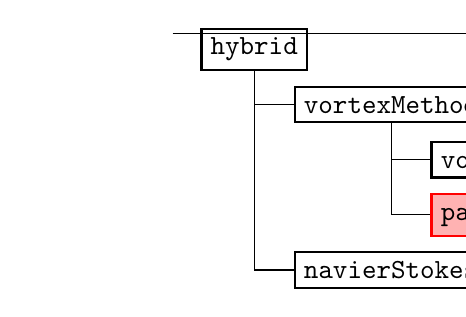
\begin{tikzpicture}[%
  grow via three points={one child at (0.5,-0.7) and
  two children at (0.5,-0.7) and (0.5,-1.4)},
  edge from parent path={(\tikzparentnode.south) |- (\tikzchildnode.west)}]
  \node {\texttt{hybrid}}
    child { node {\texttt{vortexMethod}}
    	child {node {\texttt{vortexBlobs}}}
    	child {node [selected] {\texttt{panels}}}  	
    }
    child [missing] {}				
    child [missing] {}				
    child { node {\texttt{navierStokes}}};
    %child { node [selected] {tex}
    %  child { node {generic}}
    %  child { node [optional] {latex}}
    %  child { node {plain}}
    %}
    %child [missing] {}
    %child { node {texdoc}};
\end{tikzpicture}
\end{figure}


\subsection*{Class structure:}
\begin{figure}[h]
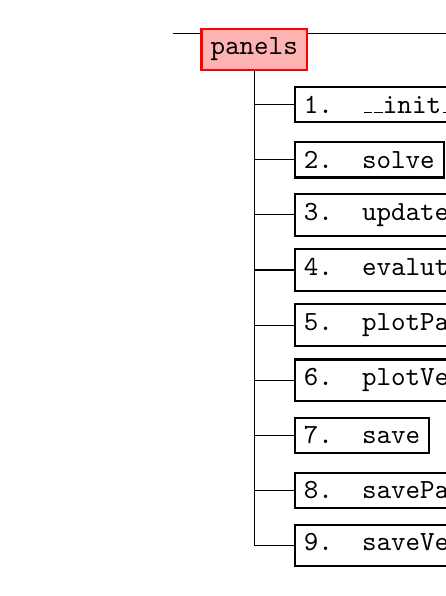
\begin{tikzpicture}[%
  grow via three points={one child at (0.5,-0.7) and
  two children at (0.5,-0.7) and (0.5,-1.4)},
  edge from parent path={(\tikzparentnode.south) |- (\tikzchildnode.west)}]
  \node [selected] {\texttt{panels}}
    child { node {\texttt{1. \_\_init\_\_}}}
    child { node {\texttt{2. solve}}}
    child { node {\texttt{3. updateBody}}}    
    child { node {\texttt{4. evaluteVelocity}}}                    
    child { node {\texttt{5. plotPanels}}}                        
    child { node {\texttt{6. plotVelocity}}}                        
    child { node {\texttt{7. save}}}                        
    child { node {\texttt{8. savePanels}}}                                        
    child { node {\texttt{9. saveVelocity}}};                                            
	%  child { node [selected] {tex}
    %  child { node {generic}}
    %  child { node [optional] {latex}}
    %  child { node {plain}}
    %}
    %child { node {texdoc}};
\end{tikzpicture}
\end{figure}

\subsection{\texttt{\_\_init\_\_}}
	\begin{tabular}{l|lp{7cm}}
		\multicolumn{2}{l}{\textbf{Input Parameters}} & \\ \hline
		\textit{File Name} & \multicolumn{2}{l}{Containing all the parameters to re-initalize the class.} \\ \hline
		\multirow{2}{*}{\textit{Parameters}} & Panel coordinates &: \{\texttt{xCP, yCP, xPanel, yPanel, cmGlobal, thetaLocal}\}\\ \cline{2-3}
		& External velocity &: \texttt{externVel} \\ \cline{2-3}
	\end{tabular}
	\paragraph{Description:} Initialize the \texttt{panels} class with the given input parameters. In the case of a multibody problem, a list of panel coordinates can be given and internally it takes care of the inter-coupling.\\
	\\
	\begin{tabular}{lp{10cm}}
				\textit{Panel coordinates} & \\ \hline
				\texttt{xCP,yCP} &:  the local $x,y$-coordinates of the panel collocation points.\\ 
				\texttt{xPanel,yPanel} &: the local coordinate of the panel edges. \textit{Note}: Should have a closed loop (end with initial point coordinates).\\ 
				\texttt{cmGlobal} &:  the position of reference points of a given panel body.\\
				\texttt{thetaLocal} &:  the rotational angles of the panel body axes w.r.t to the global $x$-axis.\\
	\end{tabular}\\ 
    \\ \\
	\begin{tabular}{lp{10cm}}
				\textit{External velocity} & \\ \hline
				\texttt{externVel} &:  Reference to an external velocity \textbf{function} acting of the panels. For the panel case, the external velocity will the induced velocity of the blobs + freestream \texttt{vortexBlob.evaluateVelocity}.\\
	\end{tabular}\\
	
		\begin{tabular}{lp{10cm}}
			\textbf{Input parameters} &: \texttt{xCP,yCP}\\ 
			\textbf{Assigns} &: \texttt{-}\\ 			
			\textbf{Returns} &: \texttt{vxCP,vyCP}\\ 					
		\end{tabular}\\

		
\subsection{\texttt{solve}}
	\paragraph{Description:} Function to solve the panel strength to satisfy no-slip condition.\\
	
		\begin{tabular}{lp{10cm}}
			\textit{Parameters} & \\ \hline
			\texttt{sPanel} &: the new strength of the panels, satisfying the no-through b.c of the body (no-slip with vortex panels.).\\
		\end{tabular} \vspace{5 mm}
		\\		
		\begin{tabular}{lp{10cm}}
			\textbf{Input parameters} &: \texttt{-}\\ 
			\textbf{Assigns} &: \texttt{sPanel}\\ 			
			\textbf{Returns} &: \texttt{-}\\ 					
		\end{tabular}		
			
		
\subsection{\texttt{updateBody}}
	\paragraph{Description:} Function to update all the panel body coordinates. This function will internally calculate the new panel coordinates \texttt{xPanel,yPanel,xCP,yCP} and rebuild the inter-induction matrix \texttt{A}.\\
	
		\begin{tabular}{lp{10cm}}
			\textit{Parameters} & \\ \hline
			\texttt{xPanel,yPanel} &: the $x,y$ panel coordinates in global.\\
			\texttt{xCP,yCP} &: the $x,y$ coordinates of the collocation point in global.\\
			\texttt{A} &: the panel self-induction matrix.
		\end{tabular} \vspace{5 mm}
		\\		
		\begin{tabular}{lp{10cm}}
			\textbf{Input parameters} &: \texttt{thetaLocals,cmGlobals}\\ 
			\textbf{Assigns} &: \texttt{A, xPanel, yPanel, xCP, yCP}\\ 			
			\textbf{Returns} &: \texttt{-}\\ 					
		\end{tabular}	

\subsection{\texttt{evaluateVelocity}}
	\paragraph{Description:} Function to evaluate the total induced velocity due to the panels and free-stream velocity (\textit{optional}).\\
	
	    \begin{tabular}{lp{10cm}}
			\textit{Parameters} & \\ \hline
			 \texttt{xTarget,yTarget} &: the $x,y$ coordinate of the target location, where the total velocity is to be evaluated.\\
			\texttt{vxTarget,vyTarget} &: the $x,y$ induced velocity of the target points in global coordinate system.\\
		\end{tabular} \vspace{5 mm}
	\\		
	\begin{tabular}{lp{10cm}}
		\textbf{Input parameters} &: \texttt{xTarget,yTarget}\\ 
		\textbf{Assigns} &: \texttt{-}\\ 			
		\textbf{Returns} &: \texttt{vxTarget,vyTarget}\\ 					
	\end{tabular}					

		
\subsection{plots \ldots}
	\paragraph{Description:} Function to plot and save (\textit{optional}) all the results in a given region or set of points.\\
	
		\begin{tabular}{lp{10cm}}
			\textit{Plot variables:} & \\ \hline
			\texttt{plotPanels} &:plot the panel coordinates at the current time instant.\\
			\texttt{plotVelocity} &: plot the velocity field.\\ 
			\texttt{plotVorticity} &: plot the vorticity field.\\ 
		\end{tabular} \vspace{5 mm}
		
		\begin{tabular}{lp{10cm}}
			\textit{Parameters:} & \\ \hline
			\texttt{xBounds,yBounds} &: $x,y$ bounds of the grid, where the data is to be evaluated and saved.\\ 
			\texttt{nGrid} &: $x,y$ number of evaluation grid points.\\ 
			\texttt{xEval,yEval} &: $x,y$ coordinates of the location where the data is to be evaluated and saved.\\ 
		\end{tabular} \vspace{5 mm}\\
	\\
	\begin{tabular}{lp{10cm}}
		\textbf{Input parameters} &: \texttt{xBounds,yBounds,hGrid} or \texttt{xEval,yEval}\\ 
		\textbf{Assigns} &: \texttt{-}\\ 			
		\textbf{Returns} &: \texttt{figureHandle} and/or \texttt{.pvd}\\ 					
	\end{tabular}	

\subsection{save data \ldots}
	\paragraph{Description:} Function to save the data in a given region or at given set of points.\\

		\begin{tabular}{lp{10cm}}
			\textit{Save variables:} & \\ \hline
			\texttt{save} &: all the data of the \texttt{panels} class, to be used to restart later.\\ 			
			\texttt{savePanels} &: the function to save the panel data at the current time instant.\\ 			
			\texttt{saveVelocity} &: save the velocity field of the given region or the given set of points.\\ 
			\texttt{saveVorticity} &: save the vorticity field of the given region or the given set of points.\\ 
		\end{tabular} \vspace{5 mm}
	
		\begin{tabular}{lp{10cm}}
			\textit{Parameters:} & \\ \hline
			\texttt{xBounds,yBounds} &: $x,y$ bounds of the grid, where the data is to be evaluated and saved.\\ 
			\texttt{nGrid} &: $x,y$ number of grid points.\\ 
			\texttt{xEval,yEval} &: $x,y$ coordinates of the location where the data is the be evaluated and saved.\\ 
		\end{tabular} \vspace{5 mm}\\
	\\
	\begin{tabular}{lp{10cm}}
		\textbf{Input parameters} &: \texttt{xBounds,yBounds,hGrid} or \texttt{xEval,yEval}\\ 
		\textbf{Assigns} &: \texttt{-}\\ 			
		\textbf{Returns} &: \texttt{.npz}\\ 					
	\end{tabular}

%
%
%\subsection{save plots \ldots}
%	\paragraph{Description:} Function to save the plots of a region or a given set of points as scientific visualization format \texttt{.pvd}.\\
%	
%		\begin{tabular}{lp{10cm}}
%			\textit{Save variables:} & \\ \hline
%			\texttt{saveVelocityPlot} &: save the velocity $\mathbf{V}$ plot.\\ 
%			\texttt{saveVorticityPlot} &: save the vorticity $\mathbf{\omega}$ plot.\\ 
%		\end{tabular} \vspace{5 mm}
%		
%		\begin{tabular}{lp{10cm}}
%			\textit{Parameters:} & \\ \hline
%			\texttt{xBounds,yBounds} &: $x,y$ bounds of the grid, where the data is to be evaluated and saved.\\ 
%			\texttt{hGrid} &: $x,y$ spacing of the evaluation grid.\\ 
%			\texttt{xEval,yEval} &: $x,y$ coordinates of the location where the data is the be evaluated and saved.\\ 
%		\end{tabular} \vspace{5 mm}\\
%	\\
%	\begin{tabular}{lp{10cm}}
%		\textbf{Input parameters} &: \texttt{xBounds,yBounds,hGrid} or \texttt{xEval,yEval} \\ 
%		\textbf{Assigns} &: \texttt{-}\\ 			
%		\textbf{Returns} &: \texttt{.pvd}\\ 					
%	\end{tabular}
%\section{\texttt{vortexMethod}}
The main structure of the \texttt{vortexBlobs} + \texttt{panels} (vortexMethod) class. This class contains all the function related to the calculations of panel with vortex blobs.

\begin{figure}[h]
\centering
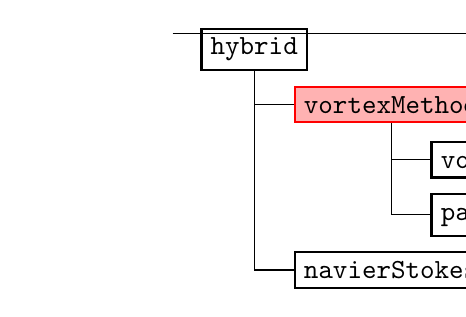
\begin{tikzpicture}[%
  grow via three points={one child at (0.5,-0.7) and
  two children at (0.5,-0.7) and (0.5,-1.4)},
  edge from parent path={(\tikzparentnode.south) |- (\tikzchildnode.west)}]
  \node {\texttt{hybrid}}
    child { node [selected] {\texttt{vortexMethod}}
    	child {node {\texttt{vortexBlobs}}}
    	child {node {\texttt{panels}}}  	
    }
    child [missing] {}				
    child [missing] {}				
    child { node {\texttt{navierStokes}}};
    %child { node [selected] {tex}
    %  child { node {generic}}
    %  child { node [optional] {latex}}
    %  child { node {plain}}
    %}
    %child [missing] {}
    %child { node {texdoc}};
\end{tikzpicture}
\end{figure}

\subsection*{Class structure:}
\begin{figure}[h]
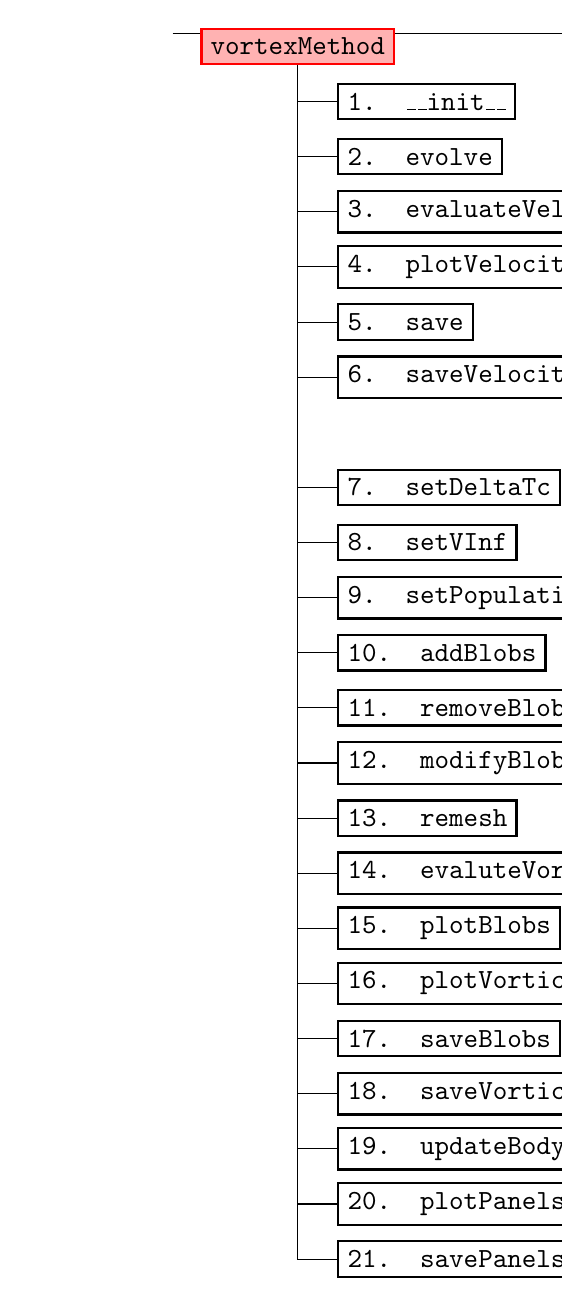
\begin{tikzpicture}[%
  grow via three points={one child at (0.5,-0.7) and
  two children at (0.5,-0.7) and (0.5,-1.4)},
  edge from parent path={(\tikzparentnode.south) |- (\tikzchildnode.west)}]
  \node [selected] {\texttt{vortexMethod}}
    child { node {\texttt{1. \_\_init\_\_}}}
    child { node {\texttt{2. evolve}}}
    child { node {\texttt{3. evaluateVelocity}}}
    child { node {\texttt{4. plotVelocity}}}                        
    child { node {\texttt{5. save}}}                        
    child { node {\texttt{6. saveVelocity}}}                                            
    child [missing] {}
    child { node {\texttt{7. setDeltaTc}}}
    child { node {\texttt{8. setVInf}}}    
    child { node {\texttt{9. setPopulationControl}}}
    child { node {\texttt{10. addBlobs}}}
    child { node {\texttt{11. removeBlobs}}}    
    child { node {\texttt{12. modifyBlobs}}}    
    child { node {\texttt{13. remesh}}}    
    child { node {\texttt{14. evaluteVorticity}}}                        
    child { node {\texttt{15. plotBlobs}}}                        
    child { node {\texttt{16. plotVorticity}}}                            
    child { node {\texttt{17. saveBlobs}}}                                        
    child { node {\texttt{18. saveVorticity}}}
    child { node {\texttt{19. updateBody}}}    
    child { node {\texttt{20. plotPanels}}}                        
    child { node {\texttt{21. savePanels}}};                                        
    	             
%    child { node {\texttt{5. plotPanels}}}                        
%    child { node {\texttt{6. plotVelocity}}}                        
%    child { node {\texttt{7. save}}}                        
%    child { node {\texttt{8. savePanels}}}                                        
%    child { node {\texttt{9. saveVelocity}}};                                            
	%  child { node [selected] {tex}
    %  child { node {generic}}
    %  child { node [optional] {latex}}
    %  child { node {plain}}
    %}
    %child { node {texdoc}};
\end{tikzpicture}
\end{figure}

%
%
%\subsection*{Class structure:}
%\begin{table}[h]
%\begin{tabular}{rl}
%	\texttt{vortexMethod}: &  \\ \hline
%	-- & \texttt{\_\_init\_\_} \\
%	& \\
%	-- & \texttt{evolve} \\ 
%	-- & \texttt{evaluateVelocity} \\ 
%	-- & \texttt{plotBlobsPanels} \\ 	
%	-- & \texttt{plotVelocity} \\ 
%	-- & \texttt{plotVorticity} \\ 	
%	-- & \texttt{saveClass} \\ 
%	-- & \texttt{saveVelocity} \\ 
%	-- & \texttt{saveVorticity} \\ 
%	-- & \texttt{saveVelocityPlot} \\ 
%	-- & \texttt{saveVorticityPlot} \\ 	
%\end{tabular}
%%\caption{\texttt{vortexMethod} class structure}
%\end{table}

\subsection{\texttt{\_\_init\_\_}}
	\begin{tabular}{l|lp{7cm}}
		\multicolumn{2}{l}{\textbf{Input Parameters}} & \\ \hline
		\textit{File Name} & \multicolumn{2}{l}{Containing all the parameters to re-initalize the class.} \\ \hline
		\multirow{2}{*}{\textit{Parameters}} & \texttt{vortexBlobs} &: \{\texttt{vortexBlobs}\} class. \\ \cline{2-3}
		& \texttt{panels} &: \texttt{panels} class. \\ \cline{2-3}
	\end{tabular}
	\paragraph{Description:} Initialize the \texttt{vortexMethod} class using \textbf{vortexBlob}+\textbf{panelMethod} classes.
	\paragraph{Input parameters:}
	\begin{list}{\quad}{}
	\item \texttt{vortexBlob}: vortex particle class
	\item \texttt{panelMethod}: panel method class				
	\end{list}

\subsection{\texttt{evolve}}
	\paragraph{Description:} Function to evolve (i.e. step) the vortex and panel together. All the necessary parameters are preassigned during the init of the vortex and panel class.\\
	
	    \begin{tabular}{lp{10cm}}
			\textit{Parameters:} & \\ \hline
			 \texttt{xBlobNew,yBlobNew,gBlobNew} &: the new $x,y$ coordinate and the new circulation $\Gamma_i$ of the blob at the new time instant.\\
			\texttt{xPanelNew,yPanelNew,sPanelNew} &: the new $x,y$ coordinates of the panel and its new strength at the new time instant.\\
		\end{tabular} \vspace{5 mm}
	\\		
	\begin{tabular}{lp{10cm}}
		\textbf{Input parameters} &: \texttt{-}\\ 
		\textbf{Assigns} &: \texttt{xBlob,yBlob,gBlob,xPanel,yPanel,sPanel}\\ 			
		\textbf{Returns} &: \texttt{-}\\ 					
	\end{tabular}

\subsection{\texttt{evaluateVelocity}}
	\paragraph{Description:} Function to evaluate the total induced velocity due to the vortex blobs, panels, and the external velocity at a given target coordinates.\\
	
	    \begin{tabular}{lp{10cm}}
			\textit{Parameters} & \\ \hline
			 \texttt{xTarget,yTarget} &: the $x,y$ coordinate of the target location, where the total velocity is to be evaluated.\\
			\texttt{vxTarget,vyTarget} &: the $x,y$ induced velocity of the target points in global coordinate system.\\
		\end{tabular} \vspace{5 mm}
	\\		
	\begin{tabular}{lp{10cm}}
		\textbf{Input parameters} &: \texttt{xTarget,yTarget}\\ 
		\textbf{Assigns} &: \texttt{-}\\ 			
		\textbf{Returns} &: \texttt{vxTarget,vyTarget}\\ 					
	\end{tabular}
		
\subsection{plots \ldots}
	\paragraph{Description:} Function to plot and save (\textit{optional}) all the results in a given region or set of points.\\
	
		\begin{tabular}{lp{10cm}}
			\textit{Plot variables:} & \\ \hline
			\texttt{plotBlobs/plotPanels} &: the plot of blobs and the panel coordinates.\\
			\texttt{plotVelocity} &: plot the velocity field of the region of the given set of points.\\ 
			\texttt{plotVorticity} &: plot the vorticity field.\\ 
		\end{tabular} \vspace{5 mm}
		
		\begin{tabular}{lp{10cm}}
			\textit{Parameters:} & \\ \hline
			\texttt{xBounds,yBounds} &: $x,y$ bounds of the grid, where the data is to be evaluated and saved.\\ 
			\texttt{nGrid} &: $x,y$ number of grid points.\\ 
			\texttt{xEval,yEval} &: $x,y$ coordinates of the location where the data is the be evaluated and saved.\\ 
		\end{tabular} \vspace{5 mm}\\
	\\
	\begin{tabular}{lp{10cm}}
		\textbf{Input parameters} &: \texttt{xBounds,yBounds,nGrid} or \texttt{xEval,yEval}\\ 
		\textbf{Assigns} &: \texttt{-}\\ 			
		\textbf{Returns} &: \texttt{figureHandle} or \texttt{saveFile}\\ 					
	\end{tabular}						

\subsection{save data \ldots}
	\paragraph{Description:} Function to save the data in a given region or at given set of points.\\

		\begin{tabular}{lp{10cm}}
			\textit{Save variables:} & \\ \hline
			\texttt{save} &: all the data of the \texttt{vortexMethod} class, to be used to restart later.\\ 			
			\texttt{saveBlobs/savePanels} &: the function to save the blobs and panel data at the current time instant.\\ 			
			\texttt{saveVelocity} &: the velocity field.\\ 
			\texttt{saveVorticity} &: the vorticity field.\\ 
		\end{tabular} \vspace{5 mm}
	
		\begin{tabular}{lp{10cm}}
			\textit{Parameters:} & \\ \hline
			\texttt{xBounds,yBounds} &: $x,y$ bounds of the grid, where the data is to be evaluated and saved.\\ 
			\texttt{nGrid} &: $x,y$ number of grid points.\\ 
			\texttt{xEval,yEval} &: $x,y$ coordinates of the location where the data is the be evaluated and saved.\\ 
		\end{tabular} \vspace{5 mm}\\
	\\
	\begin{tabular}{lp{10cm}}
		\textbf{Input parameters} &: \texttt{xBounds,yBounds,nGrid} or \texttt{xEval,yEval}\\ 
		\textbf{Assigns} &: \texttt{-}\\ 			
		\textbf{Returns} &: \texttt{.npz}\\ 					
	\end{tabular}

%\subsection{save plots \ldots}
%	\paragraph{Description:} Function to save the plots of a region or a given set of points as scientific visualization format \texttt{.pvd}.\\
%	
%		\begin{tabular}{lp{10cm}}
%			\textit{Save variables:} & \\ \hline
%			\texttt{saveVelocityPlot} &: save the velocity $\mathbf{V}$ plot.\\ 
%			\texttt{saveVorticityPlot} &: save the vorticity $\mathbf{\omega}$ plot.\\ 
%		\end{tabular} \vspace{5 mm}
%		
%		\begin{tabular}{lp{10cm}}
%			\textit{Parameters:} & \\ \hline
%			\texttt{xBounds,yBounds} &: $x,y$ bounds of the grid, where the data is to be evaluated and saved.\\ 
%			\texttt{hGrid} &: $x,y$ spacing of the evaluation grid.\\ 
%			\texttt{xEval,yEval} &: $x,y$ coordinates of the location where the data is the be evaluated and saved.\\ 
%		\end{tabular} \vspace{5 mm}\\
%	\\
%	\begin{tabular}{lp{10cm}}
%		\textbf{Input parameters} &: \texttt{xBounds,yBounds,hGrid} or \texttt{xEval,yEval} \\ 
%		\textbf{Assigns} &: \texttt{-}\\ 			
%		\textbf{Returns} &: \texttt{.pvd}\\ 					
%	\end{tabular}
%\section{\texttt{navierStokes}}
The main structure for the Navier-stokes class \texttt{navierStokes}. This class contains all the functions related to computation of the Navier-stokes problem. Below is set of functions that acts as the interface to the class.

\begin{figure}[h]
\centering
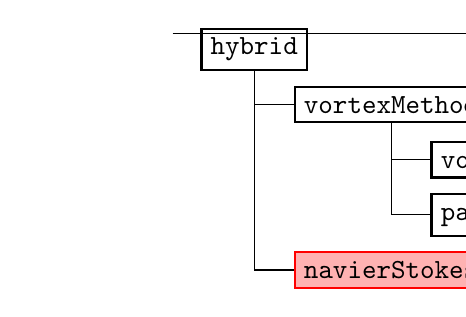
\begin{tikzpicture}[%
  grow via three points={one child at (0.5,-0.7) and
  two children at (0.5,-0.7) and (0.5,-1.4)},
  edge from parent path={(\tikzparentnode.south) |- (\tikzchildnode.west)}]
  \node {\texttt{hybrid}}
    child { node {\texttt{vortexMethod}}
    	child {node {\texttt{vortexBlobs}}}
    	child {node {\texttt{panels}}}  	
    }
    child [missing] {}				
    child [missing] {}				
    child { node [selected] {\texttt{navierStokes}}};
    %child { node [selected] {tex}
    %  child { node {generic}}
    %  child { node [optional] {latex}}
    %  child { node {plain}}
    %}
    %child [missing] {}
    %child { node {texdoc}};
\end{tikzpicture}
\end{figure}


\subsection*{Class structure:}
\begin{figure}[h]
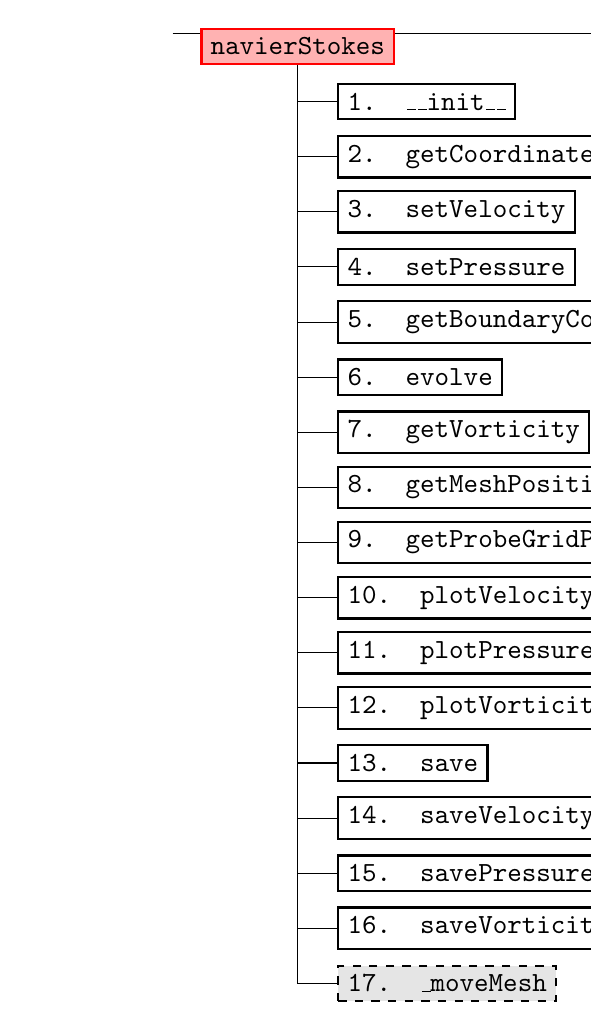
\begin{tikzpicture}[%
  grow via three points={one child at (0.5,-0.7) and
  two children at (0.5,-0.7) and (0.5,-1.4)},
  edge from parent path={(\tikzparentnode.south) |- (\tikzchildnode.west)}]
  \node [selected] {\texttt{navierStokes}}
    child { node {\texttt{1. \_\_init\_\_}}}
    child {node  {\texttt{2. getCoordinates}}}
    child { node {\texttt{3. setVelocity}}}
    child { node {\texttt{4. setPressure}}}
    child { node {\texttt{5. getBoundaryCoordinates}}}                        
    child { node {\texttt{6. evolve}}}
    child { node {\texttt{7. getVorticity}}}                        
    child { node {\texttt{8. getMeshPosition}}}                        
    child { node {\texttt{9. getProbeGridParameters}}}                        
    child { node {\texttt{10. plotVelocity}}}                        
    child { node {\texttt{11. plotPressure}}}                        
    child { node {\texttt{12. plotVorticity}}}                        
    child { node {\texttt{13. save}}}                        
    child { node {\texttt{14. saveVelocity}}}                                            
    child { node {\texttt{15. savePressure}}}                                            
    child { node {\texttt{16. saveVorticity}}}
    child { node [optional]{\texttt{17. \_moveMesh}}};
	%  child { node [selected] {tex}
    %  child { node {generic}}
    %  child { node [optional] {latex}}
    %  child { node {plain}}
    %}
    %child { node {texdoc}};
\end{tikzpicture}
\end{figure}

%\subsection*{Class structure:}
%\begin{table}[h]
%\begin{tabular}{rl}
%	\texttt{navierStokes}: &  \\ \hline
%	-- & \texttt{\_\_init\_\_} \\
%	& \\
%	-- & \texttt{initialConditions} \\ 
%	-- & \texttt{evolve} \\ 
%	-- & \texttt{boundaryCoordinates} \\ 
%	-- & \texttt{updateMesh} \\ 
%	-- & \texttt{moveMesh} \\ 
%	-- & \texttt{computeVorticity} \\ 
%	-- & \texttt{meshPosition}\\
%	-- & \texttt{probeGridParameters} \\ 	
%	-- & \texttt{plotVelocity} \\ 		
%	-- & \texttt{plotPressure} \\ 		
%	-- & \texttt{plotVorticity} \\ 			
%	-- & \texttt{saveClass} \\ 					
%	-- & \texttt{saveVelocity} \\ 		
%	-- & \texttt{savePressure} \\ 		
%	-- & \texttt{saveVorticity} \\ 	
%	-- & \texttt{saveVelocityPlot} \\ 		
%	-- & \texttt{savePressurePlot} \\ 		
%	-- & \texttt{saveVorticityPlot} \\ 	
%\end{tabular}
%%\caption{\texttt{navierStokes} class structure}
%\end{table}

\newpage

\subsection{\texttt{\_\_init\_\_}}
	\paragraph{Description:} Initialize the \texttt{navierStokes} class either using a \texttt{fileName} containing all the necessary parameter for initialization or by explicitly inputing the parameters.\\

	\begin{tabular}{l|lp{7cm}}
		\multicolumn{2}{l}{\textbf{Input Parameters}} & \\ \hline
		\textit{File Name} & \multicolumn{2}{l}{Containing all the parameters to re-initalize the class.} \\ \hline
		\multicolumn{3}{c}{-- or --} \\ \hline
		\multirow{5}{*}{\textit{Parameters}} & Mesh data &: \texttt{mesh, boundaryDomains}\\ \cline{2-3}
		& Geometry position &: \texttt{cmGlobal, thetaLocal} \\ \cline{2-3}
		& Fluid parameters &: \texttt{uMax, nu}\\ \cline{2-3}
		& Solver options &: \texttt{cfl}\\ \cline{2-3}
		& Probe grid parameters &: \texttt{x0, y0, Lx, Ly, hx, hy}\\ \cline{2-3}

	\end{tabular}\\
	\subsubsection*{Descrition of the parameters:}
	
	\begin{tabular}{lp{10cm}}
				\textit{Mesh data} & \\ \hline
				\texttt{mesh} &: the mesh data file.\\ 
				\texttt{boundaryDomains} &: the boundary mesh domain data file.\\ 			
	\end{tabular}\\ 
    \\ \\
	\begin{tabular}{lp{10cm}}
				\textit{Geometry position} & \\ \hline
				\texttt{cmGlobal} &: the $x,y$ position of the geometry in global coordinates.\\ 
				\texttt{thetaGlobal} &: the rotation angle (in $rad$) of the geometry in global coordinate system.\\ 			
	\end{tabular}\\
    \\ \\
	\begin{tabular}{lp{10cm}}
				\textit{Fluid parameters} & \\ \hline
				\texttt{uMax} &: the maximum fluid velocity $U_{max}$. Used to determine the maximum time step size $\Delta t_{max}$.\\ 
				\texttt{nu} &: the fluid kinematic viscosity $\nu$, for incompressible navier-stokes problem.\\ 			
	\end{tabular}\\	
    \\ \\
	\begin{tabular}{lp{10cm}}
				\textit{Solver options} & \\ \hline
				\texttt{cfl} &: the $CFL$ stability parameter. If explicit time marching scheme, $CFL<1$.\\ 		
	\end{tabular}\\	
    \\ \\
	\begin{tabular}{lp{10cm}}
				\textit{Probe grid parameters} & \\ \hline
				\texttt{x0,y0} &: the $x,y$ coordinate of the origin of the probe grid.\\ 
				\texttt{Lx,Ly} &: the $x,y$ size (width and height) of the probing grid.\\ 			
				\texttt{hx,hy} &: the $x,y$ spacing of the probe grid cell.\\ 							
	\end{tabular}\\	

\subsection{\texttt{getCoordinates}}
	\paragraph{Description:} Function to get all the coordinates of the velocity function spaces $\mathbf{V}$. With the returned coordinates, one could calculate the velocity field in the navier-stokes domain. \textit{Note}: The coordinates and just a list of DOF coordinate of the vector function space and is given in the same order as the data that is to be stored.\\
	
	    \begin{tabular}{lp{10cm}}
			\textit{Parameters} & \\ \hline
			\texttt{xCoordinates,yCoordinates} &: the $x,y$ coordinates of the velocity vector function space $\mathbf{V}$. \\		
		\end{tabular} \vspace{5 mm}
	\\		
	\begin{tabular}{lp{10cm}}
		\textbf{Input parameters} &: \texttt{-}\\ 
		\textbf{Assigns} &: \texttt{-}\\ 			
		\textbf{Returns} &: \texttt{xCoordinates,yCoordinates}\\ 					
	\end{tabular}

\subsection{\texttt{setVelocity}}
	\paragraph{Description:} Function to apply the current velocity field.\\
	
	    \begin{tabular}{lp{10cm}}
			\textit{Parameters} & \\ \hline
			\texttt{vFieldNew} &: the \textit{new} velocity at the navier-stokes DOF coordinates of the vector function space $\mathbf{V}$.\\		
		\end{tabular} \vspace{5 mm}
	\\		
	\begin{tabular}{lp{10cm}}
		\textbf{Input parameters} &: \texttt{vFieldNew}\\ 
		\textbf{Assigns} &: \texttt{vField}\\ 			
		\textbf{Returns} &: \texttt{-}\\ 					
	\end{tabular}
	
\subsection{\texttt{setPressure}}
	\paragraph{Description:} Function to apply the current pressure field.\\
	
	    \begin{tabular}{lp{10cm}}
			\textit{Parameters} & \\ \hline
			\texttt{pFieldNew} &: the \textit{new} pressure field at the navier-stokes DOF coordinates of the scalar function space $\mathbf{V}$.\\ 
		\end{tabular} \vspace{5 mm}
	\\		
	\begin{tabular}{lp{10cm}}
		\textbf{Input parameters} &: \texttt{pFieldNew}\\ 
		\textbf{Assigns} &: \texttt{pField}\\ 			
		\textbf{Returns} &: \texttt{-}\\ 					
	\end{tabular}

\subsection{\texttt{getBoundaryCoordinates}}
	\paragraph{Description:} Function to return the boundary DOF coordinates \texttt{xBoundary,yBoundary} of the vector function space $\mathbf{V}$.\\
	
		\begin{tabular}{lp{10cm}}
			\textit{Parameters} & \\ \hline
			\texttt{xBoundary,yBoundary} &: $x,y$ boundary coordinates of the vector function space  $\mathbf{V}$. \\ 
		\end{tabular} \vspace{5 mm}
	\\
	\begin{tabular}{lp{10cm}}
		\textbf{Input parameters} &: \texttt{-}\\ 
		\textbf{Assigns} &: \texttt{-}\\ 			
		\textbf{Returns} &: \texttt{xBoundary,yBoundary}\\ 					
	\end{tabular}	

\subsection{\texttt{evolve}}
	\paragraph{Description}: Function to evolve the Navier-stokes by one step with the $x,y$ velocity boundary condition \texttt{vxBoundary,vyBoundary} at the Navier-stokes finite element mesh boundary \texttt{xBoundary,yBoundary}. The function will calculate the new velocity and the pressure fields. The \textit{new} mesh position is used to update the mesh position, whereas the \textit{current} mesh velocity is used to calculate the modified convective term to take in account of the rigid mesh motion.\\
	
		\begin{tabular}{lp{10cm}}
			\textit{Parameters} & \\ \hline
			\texttt{vxBoundary,vyBoundary} &: $x,y$ velocity at the navier-stokes dof boundary coordinates as described by \texttt{xBoundary,yBoundary}.\\ 
			\texttt{xBoundary,yBoundary} &: $x,y$ boundary coordinates of the vector function space.\\ 
			\texttt{cmGlobalNew,thetaGlobalNew} &: the \textit{new} mesh position and the global mesh rotational angle\\
			\texttt{cmDotGlobal, thetaDotGlobal} &: the \textit{current} mesh velocities (displacement velocity and rotational velocity) in the global reference frame.\\
		\end{tabular} \vspace{5 mm}
	\\	
	\begin{tabular}{lp{10cm}}
		\textbf{Input parameters} &: \texttt{vxBoundary,vyBoundary, cmGlobalNew,thetaGlobalNew, cmDotGlobal, thetaDotGlobal}\\ 
		\textbf{Assigns} &: \texttt{vField, pField}\\ 			
		\textbf{Returns} &: \texttt{-}\\ 					
	\end{tabular}	


	

%
%\subsection{\texttt{moveMesh}}
%	\paragraph{Description:} Function to move the mesh using body displacement and rotational velocities. This function can be then used to calculate the mesh velocity of the current instant.\\
%	
%		\begin{tabular}{lp{10cm}}
%			\textit{Parameters} & \\ \hline
%			\texttt{cmDotGlobal} &: the $x,y$ global mesh coordinate displacement velocity.\\ 
%			\texttt{thetaDotGlobal} &: the polar rotational velocity of the navier-stokes domain w.r.t global coordintes.\\ 			
%			\texttt{vMesh} &: the mesh velocity w.r.t to global $x,y$-axis\\	
%		\end{tabular} \vspace{5 mm}
%	\\
%	\begin{tabular}{lp{10cm}}
%		\textbf{Input parameters} &: \texttt{cmDotGlobal,thetaDotGlobal}\\ 
%		\textbf{Assigns} &: \texttt{xBoundary,yBoundary,vMesh}\\ 			
%		\textbf{Returns} &: \texttt{-}\\ 					
%	\end{tabular}
	
	
\subsection{\texttt{getVorticity}}
	\paragraph{Description:} Function to evaluate the vorticity at probe coordinates defined by the probe mesh.\\
	
		\begin{tabular}{lp{10cm}}
			\textit{Parameters} & \\ \hline
			\texttt{vortProbeGrid} &: the vorticity $\omega$ at the probe grid coordinates \texttt{xProbeGrid, yProbeGrid}.\\ 
		\end{tabular} \vspace{5 mm}
	\\
	\begin{tabular}{lp{10cm}}
		\textbf{Input parameters} &: \texttt{-}\\ 
		\textbf{Assigns} &: \texttt{-}\\ 			
		\textbf{Returns} &: \texttt{wProbeGrid}\\ 					
	\end{tabular}


\subsection{\texttt{getMeshPosition}}

	\paragraph{Description:} Function to return the current mesh position and rotational angle.\\
	
		\begin{tabular}{lp{10cm}}
			\textit{Parameters} & \\ \hline
			\texttt{cmGlobal} &: the $x,y$ position of the mesh in global coordinates.\\ 
			\texttt{thetaGlobal} &: the rotational angle of the mesh w.r.t the global $x$ axis.\\
		\end{tabular} \vspace{5 mm}
	\\
	\begin{tabular}{lp{10cm}}
		\textbf{Input parameters} &: \texttt{-}\\ 
		\textbf{Assigns} &: \texttt{-}\\ 			
		\textbf{Returns} &: \texttt{cmGlobal,thetaGlobal}\\ 					
	\end{tabular}

\subsection{\texttt{getProbeGridParameters}}

	\paragraph{Description:} Function to return the probe grid parameters.\\
	
		\begin{tabular}{lp{10cm}}
			\textit{Parameters} & \\ \hline
			\texttt{x0,y0} &: the global $x,y$ coordinates of the probe mesh origin.\\ 
			\texttt{Lx,Ly} &: the local width and height of the probe mesh.\\
			\texttt{hx,hy} &: the probe spacing of the structure probe mesh.\\			
		\end{tabular} \vspace{5 mm}
	\\
	\begin{tabular}{lp{10cm}}
		\textbf{Input parameters} &: \texttt{-}\\ 
		\textbf{Assigns} &: \texttt{-}\\ 			
		\textbf{Returns} &: \texttt{x0,y0,Lx,Ly,hx,hy}\\ 					
	\end{tabular}

\subsection{plots \ldots}
	\paragraph{Description:} Function to plot and/or save (\textit{optional}) all the results.\\
	
		\begin{tabular}{lp{10cm}}
			\textit{Plot variables} & \\ \hline
			\texttt{plotVelocity} &: the velocity $\mathbf{V}$ of the navier-stokes domain, \texttt{u1}.\\ 
			\texttt{plotPressure} &: the pressure $\mathbf{p}$ of the navier-stokes domain, \texttt{p1}\\ 
			\texttt{plotVorticity} &: the vorticity $\mathbf{\omega}$ of the navier-stokes domain, \texttt{w1}.\\ 
		\end{tabular} \vspace{5 mm}
	\\
	\begin{tabular}{lp{10cm}}
		\textbf{Input parameters} &: \texttt{-}\\ 
		\textbf{Assigns} &: \texttt{-}\\ 			
		\textbf{Returns} &: \texttt{figureHandle} or \texttt{saveFile}\\ 					
	\end{tabular}

\subsection{save datas \ldots}
	\paragraph{Description:} Function to save the navier-stokes data as binaries.\\
	
		\begin{tabular}{lp{10cm}}
			\textit{Save variables} & \\ \hline
			\texttt{save} & : all the data of the \texttt{navierStokes} class, to be used to restart later.\\
			\texttt{saveVelocity} &: the velocity $\mathbf{V}$ of the navier-stokes domain, \texttt{u1}.\\ 
			\texttt{savePressure} &: the pressure $\mathbf{p}$ of the navier-stokes domain, \texttt{p1}\\ 
			\texttt{saveVorticity} &: the vorticity $\mathbf{\omega}$ of the navier-stokes domain, \texttt{w1}.\\ 
		\end{tabular} \vspace{5 mm}
	\\
	\begin{tabular}{lp{10cm}}
		\textbf{Input parameters} &: \texttt{-}\\ 
		\textbf{Assigns} &: \texttt{-}\\ 			
		\textbf{Returns} &: \texttt{.npz}\\ 					
	\end{tabular}

\subsection{\texttt{\_moveMesh}}
	\paragraph{Description:} \textit{Internal} function to update the mesh coordinates using the new global position and rotational angle of the body. The function will be called through \texttt{evolve}.\\
	
		\begin{tabular}{lp{10cm}}
			\textit{Parameters} & \\ \hline
			\texttt{cmGlobal} &: the $x,y$ global coordinates of the body.\\ 
			\texttt{thetaGlobal} &: the polar rotational angle of the navier-stokes domain w.r.t global $x$-coordinate axis.\\ 			
		\end{tabular} \vspace{5 mm}
	\\
	\begin{tabular}{lp{10cm}}
		\textbf{Input parameters} &: \texttt{cmGlobal,thetaGlobal}\\ 
		\textbf{Assigns} &: \texttt{xBoundary,yBoundary}\\ 			
		\textbf{Returns} &: \texttt{-}\\ 					
	\end{tabular}


%\subsection{save plots \ldots}
%	\paragraph{Description:} Function to save the navier-stokes plots are scientific visualization format \texttt{.pvd}.\\
%	
%		\begin{tabular}{lp{10cm}}
%			\textit{Save variables} & \\ \hline
%			\texttt{saveVelocityPlot} &: the velocity $\mathbf{V}$ plot of the navier-stokes domain, \texttt{u1}.\\ 
%			\texttt{savePressurePlot} &: the pressure $\mathbf{p}$ plot of the navier-stokes domain, \texttt{p1}\\ 
%			\texttt{saveVorticityPlot} &: the vorticity $\mathbf{\omega}$ plot of the navier-stokes domain, \texttt{w1}.\\ 
%		\end{tabular} \vspace{5 mm}
%	\\
%	\begin{tabular}{lp{10cm}}
%		\textbf{Input parameters} &: \texttt{-}\\ 
%		\textbf{Assigns} &: \texttt{-}\\ 			
%		\textbf{Returns} &: \texttt{.pvd}\\ 					
%	\end{tabular}
%\chapter{Hybrid Eulerian-Lagrangian Vortex Particle Method}
\label{ch:helvpm}

% Summarize the sections. : domain decomposition, coordinate systems assosciated to each
% subdomains, and the coupled evolution of the hybrid method.
% Reference to the literatures: Cottet and others, stock and daenick
% We use approach of stock based on the phd research of daeninck

	\section{Introduction to Hybrid Eulerian-Lagrangian Vortex Particle Method}
	
	The \printAcron{Hybrid Eulerian-Lagrangian Vortex Particle Method}{HELVPM} is a domain decomposition method, where the Eulerian method and the Lagrangian method solves different regions of the fluid. The domain decomposition method simply splits the domain of interest and uses appropriate method in each domain. The Eulerian formulation will be used at the near-wall region, where we need proper description of the vorticity generation at the boundary, and the Lagrangian formulation is used away from the body, where we only need to evolve the vorticity field. Figure \ref{fig:domainDecomposition} shows the decomposition of the domain to the gridded and the non-gridded region.
	
		\begin{figure}[!h]
			\centering
			\includegraphics[width=0.6\linewidth]{figures/hybrid/domainDecomposition_typical_type2-crop.pdf}
			\caption{Standard domain decomposition using Schwartz iteration for coupling the two methods. Eulerian subdomain $\Omega_E$ (near the body), and Lagrangian subdomain $\Omega_L$ (away from the body). Figure is based on Guermond (2000) \cite{Guermond2000a}.}
			\label{fig:domainDecomposition}
		\end{figure}	
	
	Several studies have already been done: Cottet and Koumoutsakos (2000a)\cite{Cottet2000a}, Guermond and Lu (2000) \cite{Guermond2000a} simulated the advection dominated flows; Ould-Salhi et al. (2001) \cite{Ould-Salihi2001a} blended the finite difference and vortex method together; Winckelmans et al. (2005a) \cite{Winckelmans2005} investigated the trailing vorticies; Daeninck (2006) \cite{Daeninck2006} used a simplified coupling strategy, coupling Vortex Particle Method and Finite Diference Method; Stock (2010) \cite{Stock2010a} expanded Daeninck's strategy, coupling Vortex Particle Method and Finite Volume Method and modeled a 3D rotor.

	\section{Convectional Coupling Strategy}
	\label{sec:helvpm-ccs}
	
	When investigating the literature works, we see that not all domain decomposition methods are the same. The main difference between the methods is their coupling strategies. Most works employ the\textit{ Schwartz alternating method} to couple the vortex particle method and the grid solver. The Schwartz alternating method (or sometimes referred to as Schwartz iterative method), couples the vortex particle method and the grid solver by iteratively determining the boundary condition such that the stream functions in both domains, $\psi_L$ and $\psi_E$ in $\Omega_L$ and $\Omega_E$ respectively, match at the overlap region $\Omega_E-\Omega_L$, shown in Figure \ref{fig:domainDecomposition}. The summary of a single iteration of the Schwartz alternating method is as follows:
	
		\begin{itemize}
		\item Determine the Eulerian boundary condition, the stream function $\psi_{\Sigma_1}$ at the Eulerian boundary $\Sigma_1$, extracted from the Lagrangian stream function $\psi_L$ in the Lagrangian subdomain $\Omega_L$.
		\item Solve for the stream function $\psi_E$ in the Eulerian subdomain $\Omega_E$ with the new boundary condition $\Sigma_1$.
		\item Determine the Lagrangian condition, the stream function $\psi_{\Sigma_0}$ at the Lagrangian boundary $\Sigma_0$, extracted from the Eulerian stream function $\psi_E$ in the Eulerian subdomain $\Omega_E$.
		\item Solve the stream function $\psi_L$ in the Lagrangian subdomain with the boundary conditions $\psi_{\Sigma_0}$ at the Lagrangian boundary $\Sigma_0$.
		\end{itemize}
	
	This procedure is iterated until the stream functions of both domains converge \cite{Ould-Salihi2001a}. Once the stream function is determined in both the domains, the velocity field can be obtained. Using the velocity field, we can then evolve the vorticity field in the Lagrangian subdomain.

	\section{Simplified Coupling Strategy}
	\label{sec:helvpm-scs}
	
	As we realized now, the downside to this procedure is that we have to solve the stream function in both $\Omega_E$ and $\Omega_L$ iteratively, until we converge to a solution. This makes the computation very expensive, especially when we are dealing with large numbers of vortex particles. Therefore, for this project, we are using the coupling technique that is based on the research work of Daeninck (2006) \cite{Daeninck2006} and Stock (2010) \cite{Stock2010a}. However, through the course of present work, we will see that we have to perform a modification to the scheme, to ensure that the total circulation of the Lagrangian domain is conserved at all times.	
	
%	\subsection{Coupling Eulerian and Lagrangian Methods}
	
	The simplified coupling strategy was first demonstrated in the doctoral thesis of Daeninck \cite{Daeninck2006}. Daeninck showed that it is possible to coupled the Lagrangian and the Eulerian method without the use of Schwartz iterative method. Daeninck proposed this approach from the following statements:
	
	\begin{itemize}
	\item The Lagrangian vortex method solves the full fluid domain $\Omega_L$ (see Figure \ref{fig:domainDecomposition_daenick}), but under-resolves the near-wall region $\Omega_E$ as it is less efficient at resolving the boundary layer of the flow.
	
	\item Eulerian method is used to resolve the near-wall region $\Omega_E$, efficiently capturing the boundary layer features and flow separation.
	
	\item The Lagrangian subdomain in the near-wall region $\Omega_L\cap\Omega_E$ is corrected using the more accurate Eulerian solutions to compensate the aforementioned under-resolution.
	
	\item The boundary conditions for the Eulerian method is directly obtained from the evolved solution of the Lagrangian method.
	\end{itemize}
	
	The grid solver therefore essentially acts as the correction for the under-resolved regions of the Lagrangian method. The Lagrangian vortex method in the full fluid domain focuses only on capturing and efficiently evolving the wake.
	
		\begin{figure}[!h]
			\centering
			\includegraphics[width=0.6\linewidth]{figures/hybrid/domainDecomposition_daenick_type2-crop.pdf}
			\caption{Modified domain decomposition \underline{without} Schwartz alternating method. Lagrangian subdomain extends up to the surface of the body. Figure is based on Daeninck (2006) \cite{Daeninck2006}.}
			\label{fig:domainDecomposition_daenick}
		\end{figure}	
	
	Furthermore, Daeninck's simplified coupling strategy handles the Lagrangian boundary condition differently from the convectional domain decomposition method. In convectional method, the shedding of the vorticity from the wall is also defined in the Lagrangian method as well. However, in Daeninck's strategy, as the Lagrangian method is under-resolved at the boundary, it cannot be used to resolve the vorticity flux at the body. Instead, the Eulerian method is used to solve vorticity generation from the wall boundary, and acts as the vorticity generator for the Lagrangian method. 
	
	For this coupling strategy to be valid, there are some assumptions that we must satisfy:

	\begin{itemize}
	\item At $t_n$ before the evolution of both method to $t_{n+1}$, the Lagrangian solution matches Eulerian solution at the boundary of the near-wall region $\Sigma_d$ (see Figure \ref{fig:domainDecomposition_daenick}).
	\item Even though the Lagrangian subdomain is under-resolved in the near-wall region, it should still be able to provide accurate boundary conditions for the Eulerian method at the external boundary $\Sigma_d$.
	\item After the evolution to $t_{n+1}$, the deviation of the Lagrangian solution (due to lack of vorticity flux at Lagrangian boundary), should be minimal.
	\end{itemize}	
	
	Daeninck's the simplified coupling strategy focused on the vorticity-velocity formulation for the Eulerian domain. However, he briefly showed that it is also possible to couple the Eulerian method with the velocity-pressure formulation. The advantage of using the velocity-pressure formulation is that it will be easier to extend to a 3D problem, unlike the vorticity-velocity formulation for the Eulerian method.
	
	\subsection{Coupling Algorithm}	
	
	The coupling of the solvers was described in one global time stepping algorithm. As the Eulerian methods suffers from a larger stability constraint on the time step, and the Lagrangian time marching is computationally more expensive, a  different time discretization for both methods was employed. The Lagrangian method and the Eulerian method had the time steps $\Delta t_L$ and $\Delta t_E=\Delta t_L/k_E$, respectively, where $k_E$ is the number of Eulerian sub-steps.
	
	Assuming that we known the solutions of both solver at $t_n$, the algorithm for the coupled time marching from $t_n$ to $t_n+\Delta t_L$ for Eulerian method (with velocity-pressure formulation) and the Lagrangian method is summarized as follows:
	
	\begin{enumerate}
	\item At $t_n$, \textbf{correct the Lagrangian solution} in the near-wall region $\Omega_L\cap\Omega_E$ from the Eulerian field, Figure \ref{fig:domainDecomposition_daenick}. The vorticity in $\Omega_E$ is determined by taking the curl of the velocity field of the Eulerian method. The vortex particles strengths are determined by interpolating the vorticity from the Eulerian grid.
	
	\item \textbf{Advance the Lagrangian method} from $t_n$ to $t_{n}+\Delta t_L$, with the corrected Lagrangian solution. Before the evolution, there exists a slip velocity at the solid wall $\Sigma_w$. Therefore, the vortex method needs to enforce the \textit{no-slip} boundary condition at the wall by computing the vortex sheet $\gamma$ that cancels this slip velocity. At the end of the evolution, classic vortex methods diffuse the computed vortex sheet to the particles but in Daeninck's work, it is handled by the Eulerian method.
	
	\item\textbf{ Determine the Eulerian boundary conditions} for the velocity field $\mathbf{u}$ at $t_{n}+\Delta t_L$ from the Lagrangian solution at $t_{n} + \Delta t_L$. The Eulerian method requires the Dirichlet velocity boundary condition at $\Sigma_d$ (the Eulerian Dirichlet velocity boundary). The velocity boundary condition at the wall boundary $\Sigma_w$ for a velocity-pressure formulation is simply the zero slip velocity. 
	
	\item \textbf{Advance the Eulerian method} from $t_n$ to $t_n + \Delta t_L$ using $k_E$ Eulerian substeps. The boundary conditions on $\mathbf{u}$ at each substep is obtained by linear interpolation of the boundary condition at $t_n$ and $t_{n} + \Delta t_L$.
	\end{enumerate}	
	
	To enhance the coupling of the Eulerian and the Lagrangian method, Daeninck further modified the Eulerian solution in the most external region of the Eulerian subdomain $\Omega_E$ from interpolation the Lagrangian solution, and observed that it provided better results. Figure \ref{fig:daeninckInterpolation} the modified adjustments regions used by Daeninck in his work.
	
	\begin{figure}[!t]
		\centering
		\includegraphics[width=0.6\linewidth]{figures/hybrid/daeninckInterpolationRegions.png}
		\caption{The domain decomposition and interpolation regions used by Daeninck \cite{Daeninck2006}. The Eulerian domain is also modified to enchace the coupling of the methods.}
		\label{fig:daeninckInterpolation}
	\end{figure}		
	
	\subsection{Lagrangian Correction Step}
	
	The coupling strategy demonstrated by Daeninck \cite{Daeninck2006}, was studied and was further extended by Stock \cite{Stock2010a}. Stock's work focused on the overlap region $\Omega_E\cap\Omega_L$ (Figure \ref{fig:domainDecomposition_daenick}) and correction of the Lagrangian solution. Following observations was determined by the work:
	
	\begin{itemize}
	\item Eulerian solution is only assumed to be correct from the body surface $\Sigma_w$ to somewhat inside of the outer Eulerian domain $\Sigma_d$. Therefore, the transfer of the Eulerian solution to the Lagrangian method should take in account of the potential inaccuracy of the Eulerian solution at the outer boundary.
	
	\item The very strong gradient in vorticity (vortex sheet) cannot be efficiently and accurately transfered to the Lagrangian method. This is especially problematic at high Reynolds number flows, and interpolating this vorticity from Eulerian method to Lagrangian method results in numerical problems. Therefore, to avoid the noise in the interpolation, the correction step has to ignore the region very near to the wall.
	\end{itemize}
	
	The resulting Lagrangian correction domain, or the interpolation domain $\Omega_I$, using Stock's coupling approach is shown in Figure \ref{fig:interpolationDomainDefinition}. The interpolation domain $\Omega_I$ is defined with an offset from the Eulerian domain boundaries $\Omega_E: \partial\Omega_E=\Sigma_w \cup \Sigma_d$, Figure \ref{fig:interpolationDomainExpanded}, such that regions of the Eulerian domain that introduces issues with coupling are ignored. The outer boundary of the interpolation domain $\Sigma_i$ is defined with an offset $d_{bdry}$ from the Eulerian Dirichlet velocity boundary $\Sigma_d$ such that potential inaccuracy of the Eulerian solution is ignored, shown in Figure \ref{fig:interpolationDomainCloseup}. Similarly, the inner boundary of the interpolation domain $\Sigma_o$ is defined with an offset $d_{surf}$ from the Eulerian wall boundary $\Sigma_w$ such that the very strong vorticity is ignored. The offsets $d_{surf}$ and $d_{bdry}$  where defined in the order of the Lagrangian vortex particle size.
	
	\begin{figure}[!t]
        \centering
        \begin{subfigure}[b]{0.45\textwidth}
                \includegraphics[width=\textwidth]{figures/hybrid/interpolationDomain/interpolationDomainExpanded-crop.pdf}
                \caption{Definition of the Domains}
                \label{fig:interpolationDomainExpanded}
        \end{subfigure}%
        \qquad %add desired spacing between images, e. g. ~, \quad, \qquad etc.
          %(or a blank line to force the subfigure onto a new line)
        \begin{subfigure}[b]{0.45\textwidth}
                \includegraphics[width=\textwidth]{figures/hybrid/interpolationDomain/interpolationDomainCloseup-crop.pdf}
                \caption{Definition of the boundaries}
                \label{fig:interpolationDomainCloseup}
        \end{subfigure}
        \caption{Definition of the interpolation domain $\Omega_{int}$ for correcting the Lagrangian solution, with boundaries $\Omega_I: \partial\Omega_I=\Sigma_{i}\cup\Sigma_{o}$.}
        \label{fig:interpolationDomainDefinition}
	\end{figure}		

	The resulting Lagrangian correction step employed by Stock is summarized as follows:
	
	\begin{enumerate}
	\item Interpolate the vorticity of the Eulerian method from a non-uniformly structured (or an unstructured grid) onto a temporary uniformly structured Cartesian grid covering the entire Eulerian domain $\Omega_E$. This is done to performed an easier correction of the Lagrangian solution with the Eulerian solution. The interpolation ignores the very strong vorticity present in the boundary layer that could cause numerical problem.
	\item Determine all the particles within the interpolation domain $\Omega_I$ that is to be corrected.
	\item Correct or reset the strengths of the particles using the local particle area and the vorticity interpolated from the temporary structured Cartesian grid.
	\end{enumerate}
	
	Using this approach, Stock demonstrated the feasibility of simulating a 3D compressible flow problem around a sphere at $Re=100$, a finite airfoil at $Re=\num{1.5e6}$, and 4-Bladed advancing rotor at $Re=865,500$.
	
	\section{Evolution of the Hybrid Method}

	In the present work, we will therefore employ Daeninck's simplified coupling strategy with the detailed Lagrangian correction approach of the Stock. The evolution of the hybrid method is classified into four parts and is as follows:

		\begin{enumerate}
		\item \textbf{Correct Lagrangian:} Use the solution of the Eulerian subdomain $\Omega_E$, to correct the solution of the Lagrangian subdomain $\Omega_L$, using the strategy of Stock. Chapter \ref{ch:coupling} provides a detailed investigation on the implementation of Stock's Lagrangian correction strategy. However, during the implementation, we saw that conservation of total circulation in the Lagrangian method is paramount for an accurate correction.
		
		\item \textbf{Evolve Lagrangian:} With the modified solution, evolve the Lagrangian solution from time step $t_n$ to $t_{n}+\Delta t_L$. Chapter \ref{ch:lagrangian} provides the detailed investigation on the theory and the algorithm of the Lagrangian method used for the present work.
		
		\item \textbf{Determine Eulerian boundary conditions:} Use the Lagrangian solution of time $t_{n}+\Delta t_L$ to determine the boundary conditions of the Eulerian subdomain at $t_{n}+\Delta t_L$.
		
		\item \textbf{Evolve Eulerian:} With the boundary condition, evolve the Eulerian solution from $t_n$ to $t_{n}+\Delta t_L$ using $k_E$ Eulerian substeps. Chapter \ref{ch:eulerian} provides the detailed investigation on the theory and the algorithm of the Eulerian method used for the present work.
		\end{enumerate}
	
	Figure \ref{fig:flowchart_simpleCoupling} shows the flowchart of the evolution of the hybrid method. To ensure that the coupling of the hybrid method performs as explained in theory, we required a verification and validation test on the functionality of each segregate methods.
	
	
	\begin{figure}[!t]
		\centering
		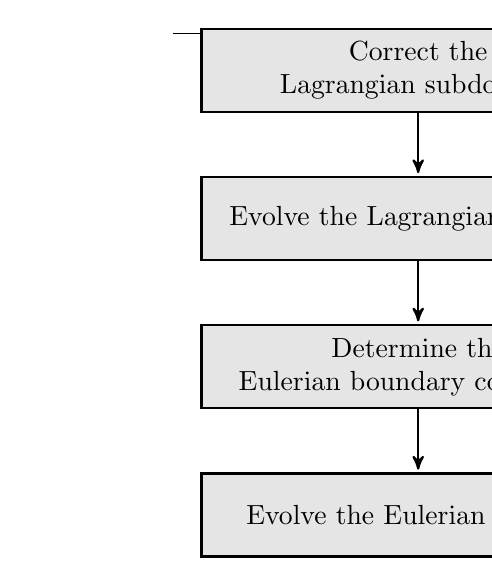
\begin{tikzpicture}
			[node distance=.8cm, start chain=going below,]
			\node[punktchain, join] (correct) {Correct the \\Lagrangian subdomain};
		    \node[punktchain, join] (evolveL) {Evolve the Lagrangian solution};
		    \node[punktchain, join] (bcE)     {Determine the \\Eulerian boundary conditions};
		    \node[punktchain, join] (evolveE) {Evolve the Eulerian solution};
		\end{tikzpicture}
		\caption{Flowchart of the simple coupling strategy. The flowchart shows the procedure to evolve both methods from $t_n$ to $t_{n+1}$.}
		\label{fig:flowchart_simpleCoupling}
	\end{figure}




% Summarize daenincks approach:
	% Methodology, algorithm
	% Domain decomposition
% Summarize stock's approach:
	% Methodology, algorithms
	% Resulted domain decomposition.


%%%%%%%%%%%%%%%%%%%%%%%%%%%%%%%%%%%%%%%%%%%%%%%%%%%%%%%%%%%%%%%%%%%%%%%%%%%%%%%%%%%%%%%%%%%%%%%%%%%%%%%%%%%%%%%%%%%%%%%%%%%%%%%%%%



%
    %\addtocontents{toc}{\protect\setcounter{tocdepth}{0}}
    %\chapter{Feasibility of hybrid vortex method for compressor cascade}
	%\appendixpage
    %\addcontentsline{toc}{chapter}{Appendices}
	%\appendix
	%\addcontentsline{toc}{chapter}{Appendix}
	%\input{appendices/main}

\backmatter%

    % index file here (not needed for a MSc thesis)
	%\printindex
	
\end{document}
